% Options for packages loaded elsewhere
\PassOptionsToPackage{unicode}{hyperref}
\PassOptionsToPackage{hyphens}{url}
%
\documentclass[
]{book}
\usepackage{amsmath,amssymb}
\usepackage{iftex}
\ifPDFTeX
  \usepackage[T1]{fontenc}
  \usepackage[utf8]{inputenc}
  \usepackage{textcomp} % provide euro and other symbols
\else % if luatex or xetex
  \usepackage{unicode-math} % this also loads fontspec
  \defaultfontfeatures{Scale=MatchLowercase}
  \defaultfontfeatures[\rmfamily]{Ligatures=TeX,Scale=1}
\fi
\usepackage{lmodern}
\ifPDFTeX\else
  % xetex/luatex font selection
\fi
% Use upquote if available, for straight quotes in verbatim environments
\IfFileExists{upquote.sty}{\usepackage{upquote}}{}
\IfFileExists{microtype.sty}{% use microtype if available
  \usepackage[]{microtype}
  \UseMicrotypeSet[protrusion]{basicmath} % disable protrusion for tt fonts
}{}
\makeatletter
\@ifundefined{KOMAClassName}{% if non-KOMA class
  \IfFileExists{parskip.sty}{%
    \usepackage{parskip}
  }{% else
    \setlength{\parindent}{0pt}
    \setlength{\parskip}{6pt plus 2pt minus 1pt}}
}{% if KOMA class
  \KOMAoptions{parskip=half}}
\makeatother
\usepackage{xcolor}
\usepackage{color}
\usepackage{fancyvrb}
\newcommand{\VerbBar}{|}
\newcommand{\VERB}{\Verb[commandchars=\\\{\}]}
\DefineVerbatimEnvironment{Highlighting}{Verbatim}{commandchars=\\\{\}}
% Add ',fontsize=\small' for more characters per line
\usepackage{framed}
\definecolor{shadecolor}{RGB}{248,248,248}
\newenvironment{Shaded}{\begin{snugshade}}{\end{snugshade}}
\newcommand{\AlertTok}[1]{\textcolor[rgb]{0.94,0.16,0.16}{#1}}
\newcommand{\AnnotationTok}[1]{\textcolor[rgb]{0.56,0.35,0.01}{\textbf{\textit{#1}}}}
\newcommand{\AttributeTok}[1]{\textcolor[rgb]{0.13,0.29,0.53}{#1}}
\newcommand{\BaseNTok}[1]{\textcolor[rgb]{0.00,0.00,0.81}{#1}}
\newcommand{\BuiltInTok}[1]{#1}
\newcommand{\CharTok}[1]{\textcolor[rgb]{0.31,0.60,0.02}{#1}}
\newcommand{\CommentTok}[1]{\textcolor[rgb]{0.56,0.35,0.01}{\textit{#1}}}
\newcommand{\CommentVarTok}[1]{\textcolor[rgb]{0.56,0.35,0.01}{\textbf{\textit{#1}}}}
\newcommand{\ConstantTok}[1]{\textcolor[rgb]{0.56,0.35,0.01}{#1}}
\newcommand{\ControlFlowTok}[1]{\textcolor[rgb]{0.13,0.29,0.53}{\textbf{#1}}}
\newcommand{\DataTypeTok}[1]{\textcolor[rgb]{0.13,0.29,0.53}{#1}}
\newcommand{\DecValTok}[1]{\textcolor[rgb]{0.00,0.00,0.81}{#1}}
\newcommand{\DocumentationTok}[1]{\textcolor[rgb]{0.56,0.35,0.01}{\textbf{\textit{#1}}}}
\newcommand{\ErrorTok}[1]{\textcolor[rgb]{0.64,0.00,0.00}{\textbf{#1}}}
\newcommand{\ExtensionTok}[1]{#1}
\newcommand{\FloatTok}[1]{\textcolor[rgb]{0.00,0.00,0.81}{#1}}
\newcommand{\FunctionTok}[1]{\textcolor[rgb]{0.13,0.29,0.53}{\textbf{#1}}}
\newcommand{\ImportTok}[1]{#1}
\newcommand{\InformationTok}[1]{\textcolor[rgb]{0.56,0.35,0.01}{\textbf{\textit{#1}}}}
\newcommand{\KeywordTok}[1]{\textcolor[rgb]{0.13,0.29,0.53}{\textbf{#1}}}
\newcommand{\NormalTok}[1]{#1}
\newcommand{\OperatorTok}[1]{\textcolor[rgb]{0.81,0.36,0.00}{\textbf{#1}}}
\newcommand{\OtherTok}[1]{\textcolor[rgb]{0.56,0.35,0.01}{#1}}
\newcommand{\PreprocessorTok}[1]{\textcolor[rgb]{0.56,0.35,0.01}{\textit{#1}}}
\newcommand{\RegionMarkerTok}[1]{#1}
\newcommand{\SpecialCharTok}[1]{\textcolor[rgb]{0.81,0.36,0.00}{\textbf{#1}}}
\newcommand{\SpecialStringTok}[1]{\textcolor[rgb]{0.31,0.60,0.02}{#1}}
\newcommand{\StringTok}[1]{\textcolor[rgb]{0.31,0.60,0.02}{#1}}
\newcommand{\VariableTok}[1]{\textcolor[rgb]{0.00,0.00,0.00}{#1}}
\newcommand{\VerbatimStringTok}[1]{\textcolor[rgb]{0.31,0.60,0.02}{#1}}
\newcommand{\WarningTok}[1]{\textcolor[rgb]{0.56,0.35,0.01}{\textbf{\textit{#1}}}}
\usepackage{longtable,booktabs,array}
\usepackage{calc} % for calculating minipage widths
% Correct order of tables after \paragraph or \subparagraph
\usepackage{etoolbox}
\makeatletter
\patchcmd\longtable{\par}{\if@noskipsec\mbox{}\fi\par}{}{}
\makeatother
% Allow footnotes in longtable head/foot
\IfFileExists{footnotehyper.sty}{\usepackage{footnotehyper}}{\usepackage{footnote}}
\makesavenoteenv{longtable}
\usepackage{graphicx}
\makeatletter
\def\maxwidth{\ifdim\Gin@nat@width>\linewidth\linewidth\else\Gin@nat@width\fi}
\def\maxheight{\ifdim\Gin@nat@height>\textheight\textheight\else\Gin@nat@height\fi}
\makeatother
% Scale images if necessary, so that they will not overflow the page
% margins by default, and it is still possible to overwrite the defaults
% using explicit options in \includegraphics[width, height, ...]{}
\setkeys{Gin}{width=\maxwidth,height=\maxheight,keepaspectratio}
% Set default figure placement to htbp
\makeatletter
\def\fps@figure{htbp}
\makeatother
\setlength{\emergencystretch}{3em} % prevent overfull lines
\providecommand{\tightlist}{%
  \setlength{\itemsep}{0pt}\setlength{\parskip}{0pt}}
\setcounter{secnumdepth}{5}
\usepackage{booktabs}
\usepackage{longtable}
\usepackage{array}
\usepackage{multirow}
\usepackage{wrapfig}
\usepackage{float}
\usepackage{colortbl}
\usepackage{pdflscape}
\usepackage{tabu}
\usepackage{threeparttable}
\usepackage{threeparttablex}
\usepackage[normalem]{ulem}
\usepackage{makecell}
\usepackage{xcolor}
\usepackage{caption}
\usepackage{anyfontsize}
\ifLuaTeX
  \usepackage{selnolig}  % disable illegal ligatures
\fi
\usepackage[]{natbib}
\bibliographystyle{apalike}
\usepackage{bookmark}
\IfFileExists{xurl.sty}{\usepackage{xurl}}{} % add URL line breaks if available
\urlstyle{same}
\hypersetup{
  pdftitle={Tutorials for BIOL202: Introduction to Biostatistics},
  pdfauthor={Jason Pither},
  hidelinks,
  pdfcreator={LaTeX via pandoc}}

\title{Tutorials for BIOL202: Introduction to Biostatistics}
\author{Jason Pither}
\date{2024-11-26}

\begin{document}
\maketitle

{
\setcounter{tocdepth}{1}
\tableofcontents
}
\part*{Preface}\label{part-preface}
\addcontentsline{toc}{part}{Preface}

\chapter*{Welcome}\label{welcome}
\addcontentsline{toc}{chapter}{Welcome}

This is an open source online book that, in one capacity, provides tutorials and other resources for the lab portion of the course BIOL202: Introduction to Biostatistics, at the University of British Columbia, Okanagan campus. Its other role is to serve as a general resource for those wishing to learn how to manage and analyze data using R and R Markdown within the RStudio IDE.

This book is \textbf{a living document that is updated intermittently.} If you find errors or wish to provide feedback, please feel free to \href{https://jasonpither.weebly.com/people.html}{contact me}.

\section*{Author}\label{author}
\addcontentsline{toc}{section}{Author}

I (Jason Pither) am an Associate Professor in the Department of Biology at the Okanagan campus of the University of British Columbia. I am an ecologist with interests in biogeography, community ecology, and landscape ecology. I have been using ``R'' (and its \href{https://en.wikipedia.org/wiki/R_(programming_language)\#History}{predecessor, ``S''}) in my research for over two decades, and have been teaching Introductory Biostatistics using R since 2014.

\section*{Acknowledgments}\label{acknowledgments}
\addcontentsline{toc}{section}{Acknowledgments}

I am grateful to be able to live, work, and play on the traditional, ancestral, and unceded territory of the Syilx (Okanagan) people. To find out more about Indigenous territories where you live, consult \url{https://native-land.ca}.

This online book borrows some material generously made openly available by the following keen educators:

\begin{itemize}
\tightlist
\item
  Chester Ismay and Albert Y. Kim (\href{https://moderndive.com/}{Statistical Inference via Data Science online book}). This resource is licensed under a \href{http://creativecommons.org/licenses/by-nc-sa/4.0/}{Creative Commons Attribution - NonCommercial-ShareAlike 4.0 International License}.
\item
  Mike Whitlock and Dolph Schluter (\href{https://whitlockschluter3e.zoology.ubc.ca/index.html}{resources accompanying the text ``Analysis of Biological Data''})
\end{itemize}

It has also benefited from valuable input from the many BIOL202 students and teaching assistants who have helped me over the years. Thank you!

Clerissa Copeland, Jordan Katchen, and Mathew Vis-Dunbar helped with some of the content development and with identifying links to other UBCO Biology material. Thanks!

\section*{Copyright}\label{copyright}
\addcontentsline{toc}{section}{Copyright}

This work is licensed under the Creative Commons \href{https://creativecommons.org/licenses/by-nc-sa/4.0/}{Attribution-NonCommercial-ShareAlike 4.0 International (CC BY-NC-SA 4.0)}


\includegraphics{./more/creative-commons-783531_1280.png}

Please use the following for citing this document

Pither, J. (2022). \emph{Tutorials for BIOL202: Introduction to Biostatistics}. \url{https://ubco-biology.github.io/BIOL202/index.html}

All source files are available on \href{https://github.com/ubco-biology/BIOL202}{github}.

\section*{UBCO Biology open materials}\label{ubco-biology-open-materials}
\addcontentsline{toc}{section}{UBCO Biology open materials}

This resource is part of a larger project to host UBCO Biology lab materials in an open, accessible format.

All BIOL open materials can be found at \url{https://ubco-biology.github.io/}

\part*{Getting started with R, RStudio \& R Markdown}\label{part-getting-started-with-r-rstudio-r-markdown}
\addcontentsline{toc}{part}{Getting started with R, RStudio \& R Markdown}

\chapter{What are R and RStudio?}\label{what_is_R}

It is assumed that you are using R via RStudio. First time users often confuse the two. At its simplest:

\begin{itemize}
\tightlist
\item
  R is like a car's engine
\item
  RStudio is like a car's dashboard.
\end{itemize}

\begin{figure}
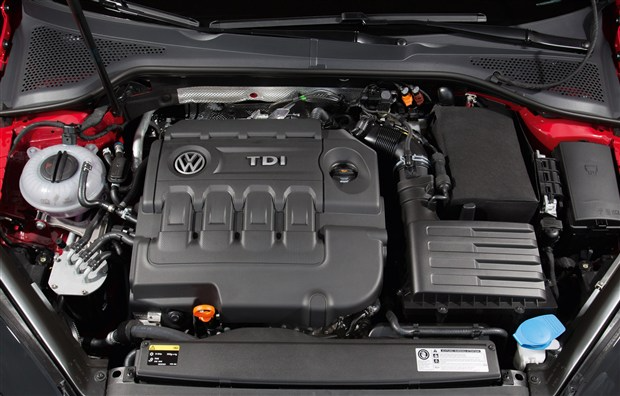
\includegraphics[width=0.3\linewidth]{./more/engine} \caption{R: Engine}\label{fig:unnamed-chunk-2}
\end{figure}

\begin{figure}
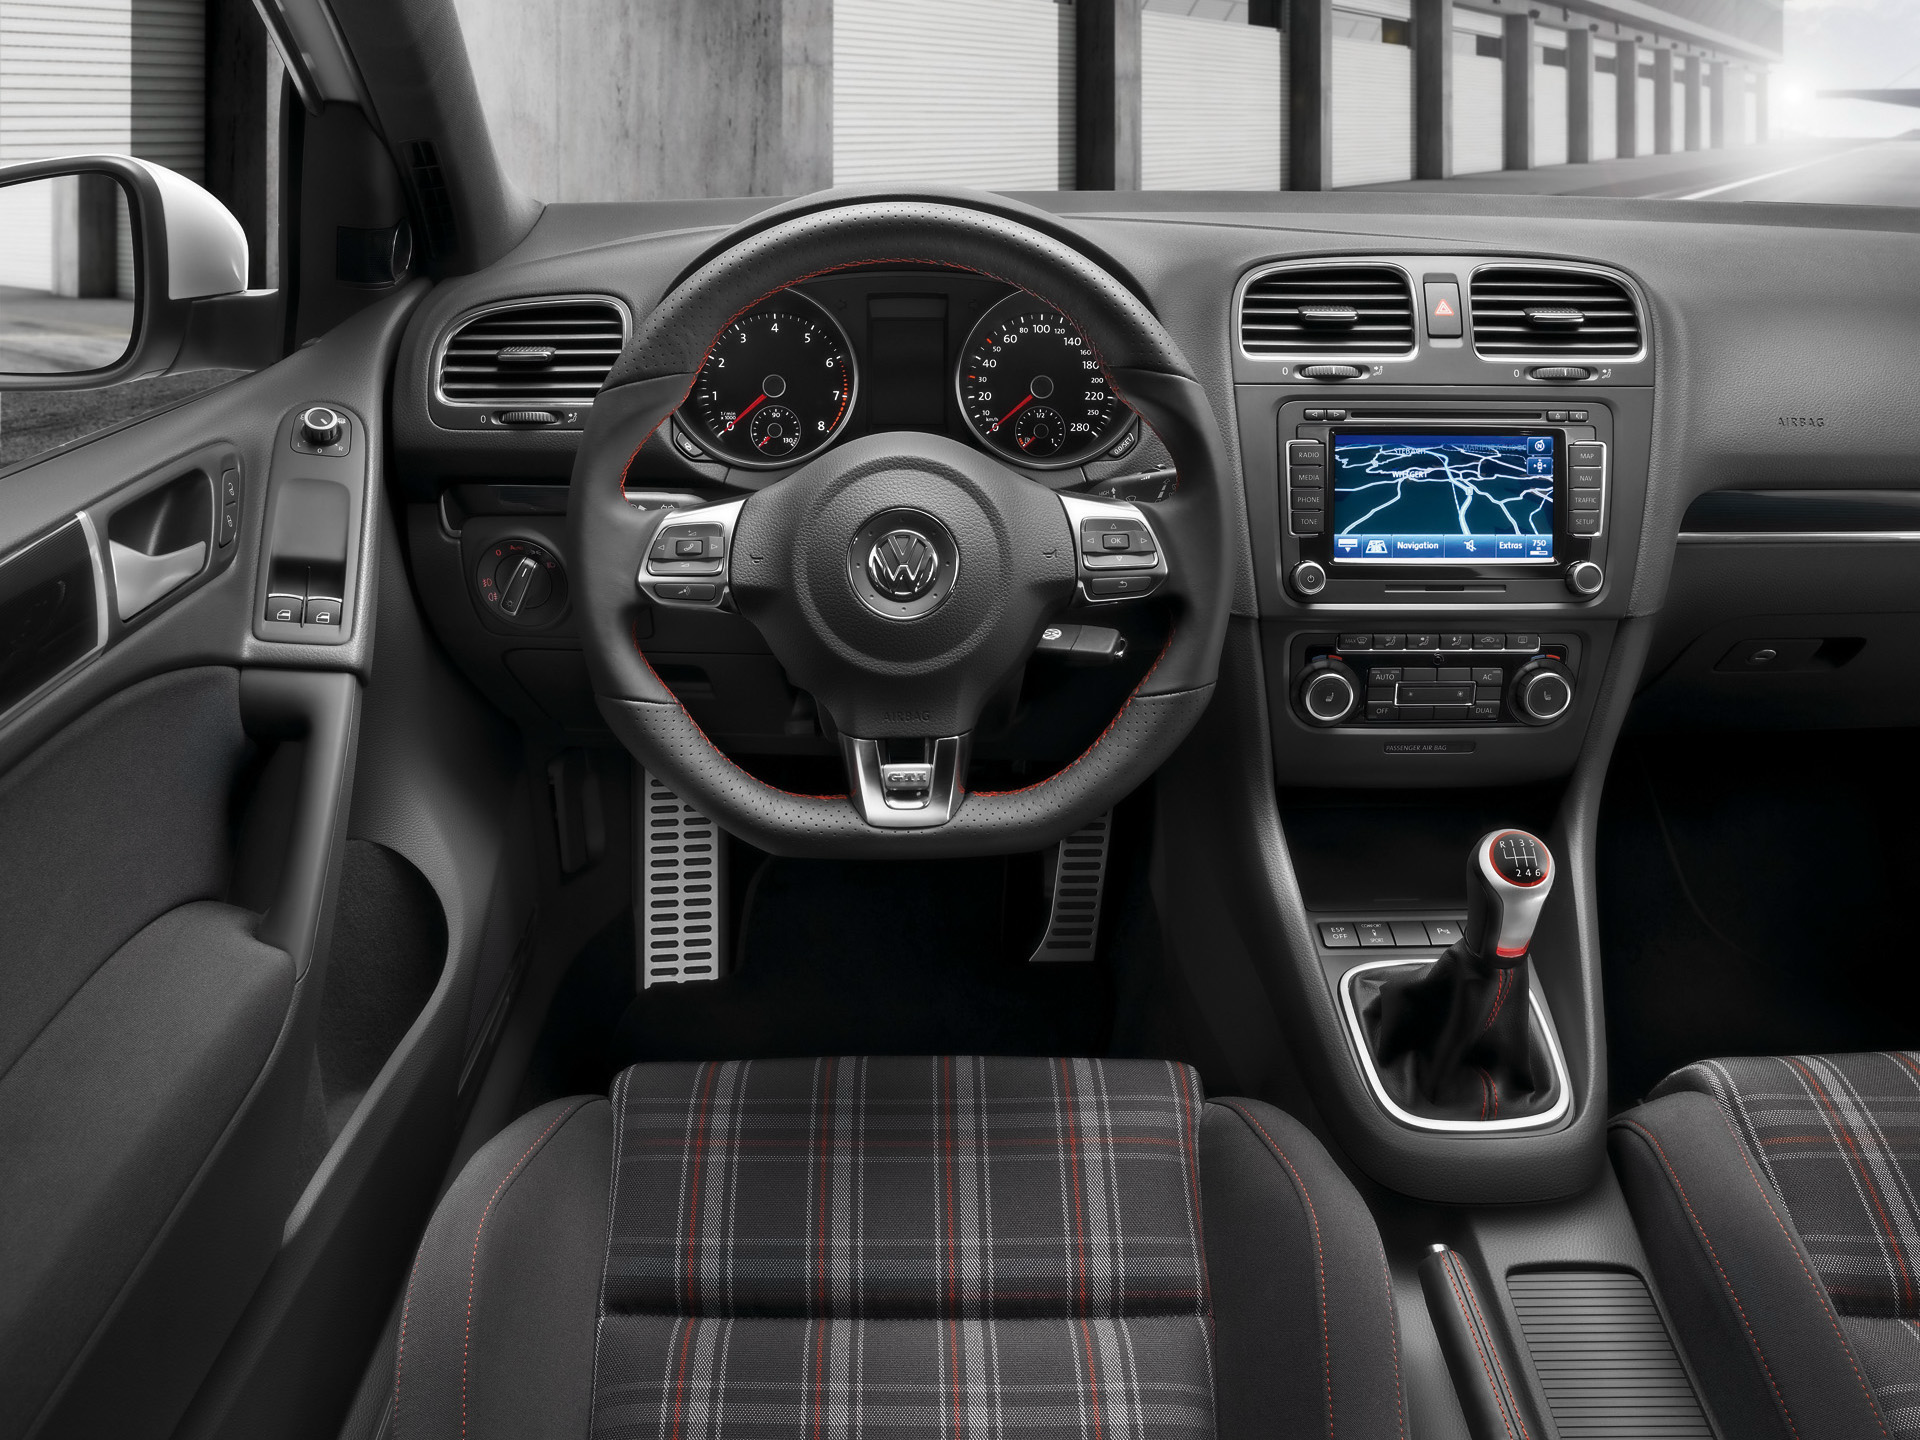
\includegraphics[width=0.2\linewidth]{./more/dashboard} \caption{RStudio: Dashboard}\label{fig:unnamed-chunk-3}
\end{figure}

More precisely, R is a programming language that runs computations while RStudio is an \emph{integrated development environment (IDE)} that provides an interface by adding many convenient features and tools. So the way of having access to a speedometer, rearview mirrors, and a navigation system makes driving much easier, using RStudio's interface makes using R much easier as well.

\section{Installing R and RStudio}\label{install_R_Rstudio}

At the time of writing this module, the latest version of R was 4.3.1 (``Beagle Scouts'') (2023-06-16). At the beginning of term, it is recommended that you update to the latest version of R, but once you've started into the tutorials, it is recommended that you NOT update again until after term is complete. This is to avoid any unforeseen problems introduced by the update. \textbf{However} If you have an older operating system on your computer, you'll want to check compatibility of both R and RStudio.

RStudio is now owned by ``posit'', and its website (posit.co) should detect your operating system and provide the appropriate download option automatically. The website with older versions of R is \href{https://cran.r-project.org/bin/macosx/}{here}, and older versions of RStudio is \href{https://docs.posit.co/previous-versions/rstudio/}{here}.

Follow the instructions below, and you are encouraged to view this YouTube video \href{https://www.youtube.com/watch?v=tgPuB-iNww0}{here} \emph{prior} to starting the steps. It talks about installing for different operating systems and different vintages of Macs (e.g.~newer M1 chips versus Intel chips).

\begin{itemize}
\tightlist
\item
  Download and install both R and RStudio (Desktop version) on your computer.
\end{itemize}

R needs to be installed successfully \textgreater prior\textless{} to installing RStudio (because the latter depends on the former)

\begin{itemize}
\tightlist
\item
  Figure out what operating system (and version) you have on your computer (e.g.~Windows 10; Mac OS X 12.51 ``Monterey'')\\
\item
  Go to this \href{https://cran.r-project.org/}{website} and click on the appropriate download link at the top of the page (depending on your operating system, Windows / MacOS / Linux)

  \begin{itemize}
  \tightlist
  \item
    For \emph{Windows} users, download the ``base'' version; this file will be called something like R-4.1.1-win.exe. Executing this file launches a familiar Windows Setup Wizard that will install R on your computer.\\
  \item
    For \emph{Mac} users, download the ``pkg'' file that is appropriate for your version of MacOS; the file will be called something like R-4.1.1.pkg. Download and run this installation package---just accept the default options and you will be ready to go.
  \end{itemize}
\item
  Now to install RStudio: once you have installed ``R'', go to this \href{https://rstudio.com/products/rstudio/download/}{website} and click on the ``download'' button in the top right corner, then select the blue button underneath the ``RStudio Desktop FREE'' column. Then, click on the appropriate link under the ``Installers for Supported Platforms'' heading; this again depends on what platform / operating system you're using. It will likely be one of the first two options.
\end{itemize}

\chapter{Start using R \& RStudio}\label{start_r}

Recall our car analogy from a \hyperref[what_is_R]{previous tutorial}. Much as we don't drive a car by interacting directly with the engine but rather by using elements on the car's dashboard, we won't be using R directly but rather we will use RStudio's interface. After you install R and RStudio on your computer, you'll have two new programs AKA applications you can open. We will always work in RStudio and not R. In other words:

\begin{figure}

\includegraphics[width=0.3\linewidth]{./more/Rlogo} \caption{R: DO NOT OPEN THIS}\label{fig:unnamed-chunk-4}
\end{figure}

\begin{figure}

\includegraphics[width=0.3\linewidth]{./more/RStudio-Ball} \caption{RStudio: OPEN THIS}\label{fig:unnamed-chunk-5}
\end{figure}

Launch RStudio on your computer to make sure it's working (it loads R for you in the background).

\section{The RStudio Interface}\label{Rstudio_interface}

When you open RStudio, you should see something similar to the following:

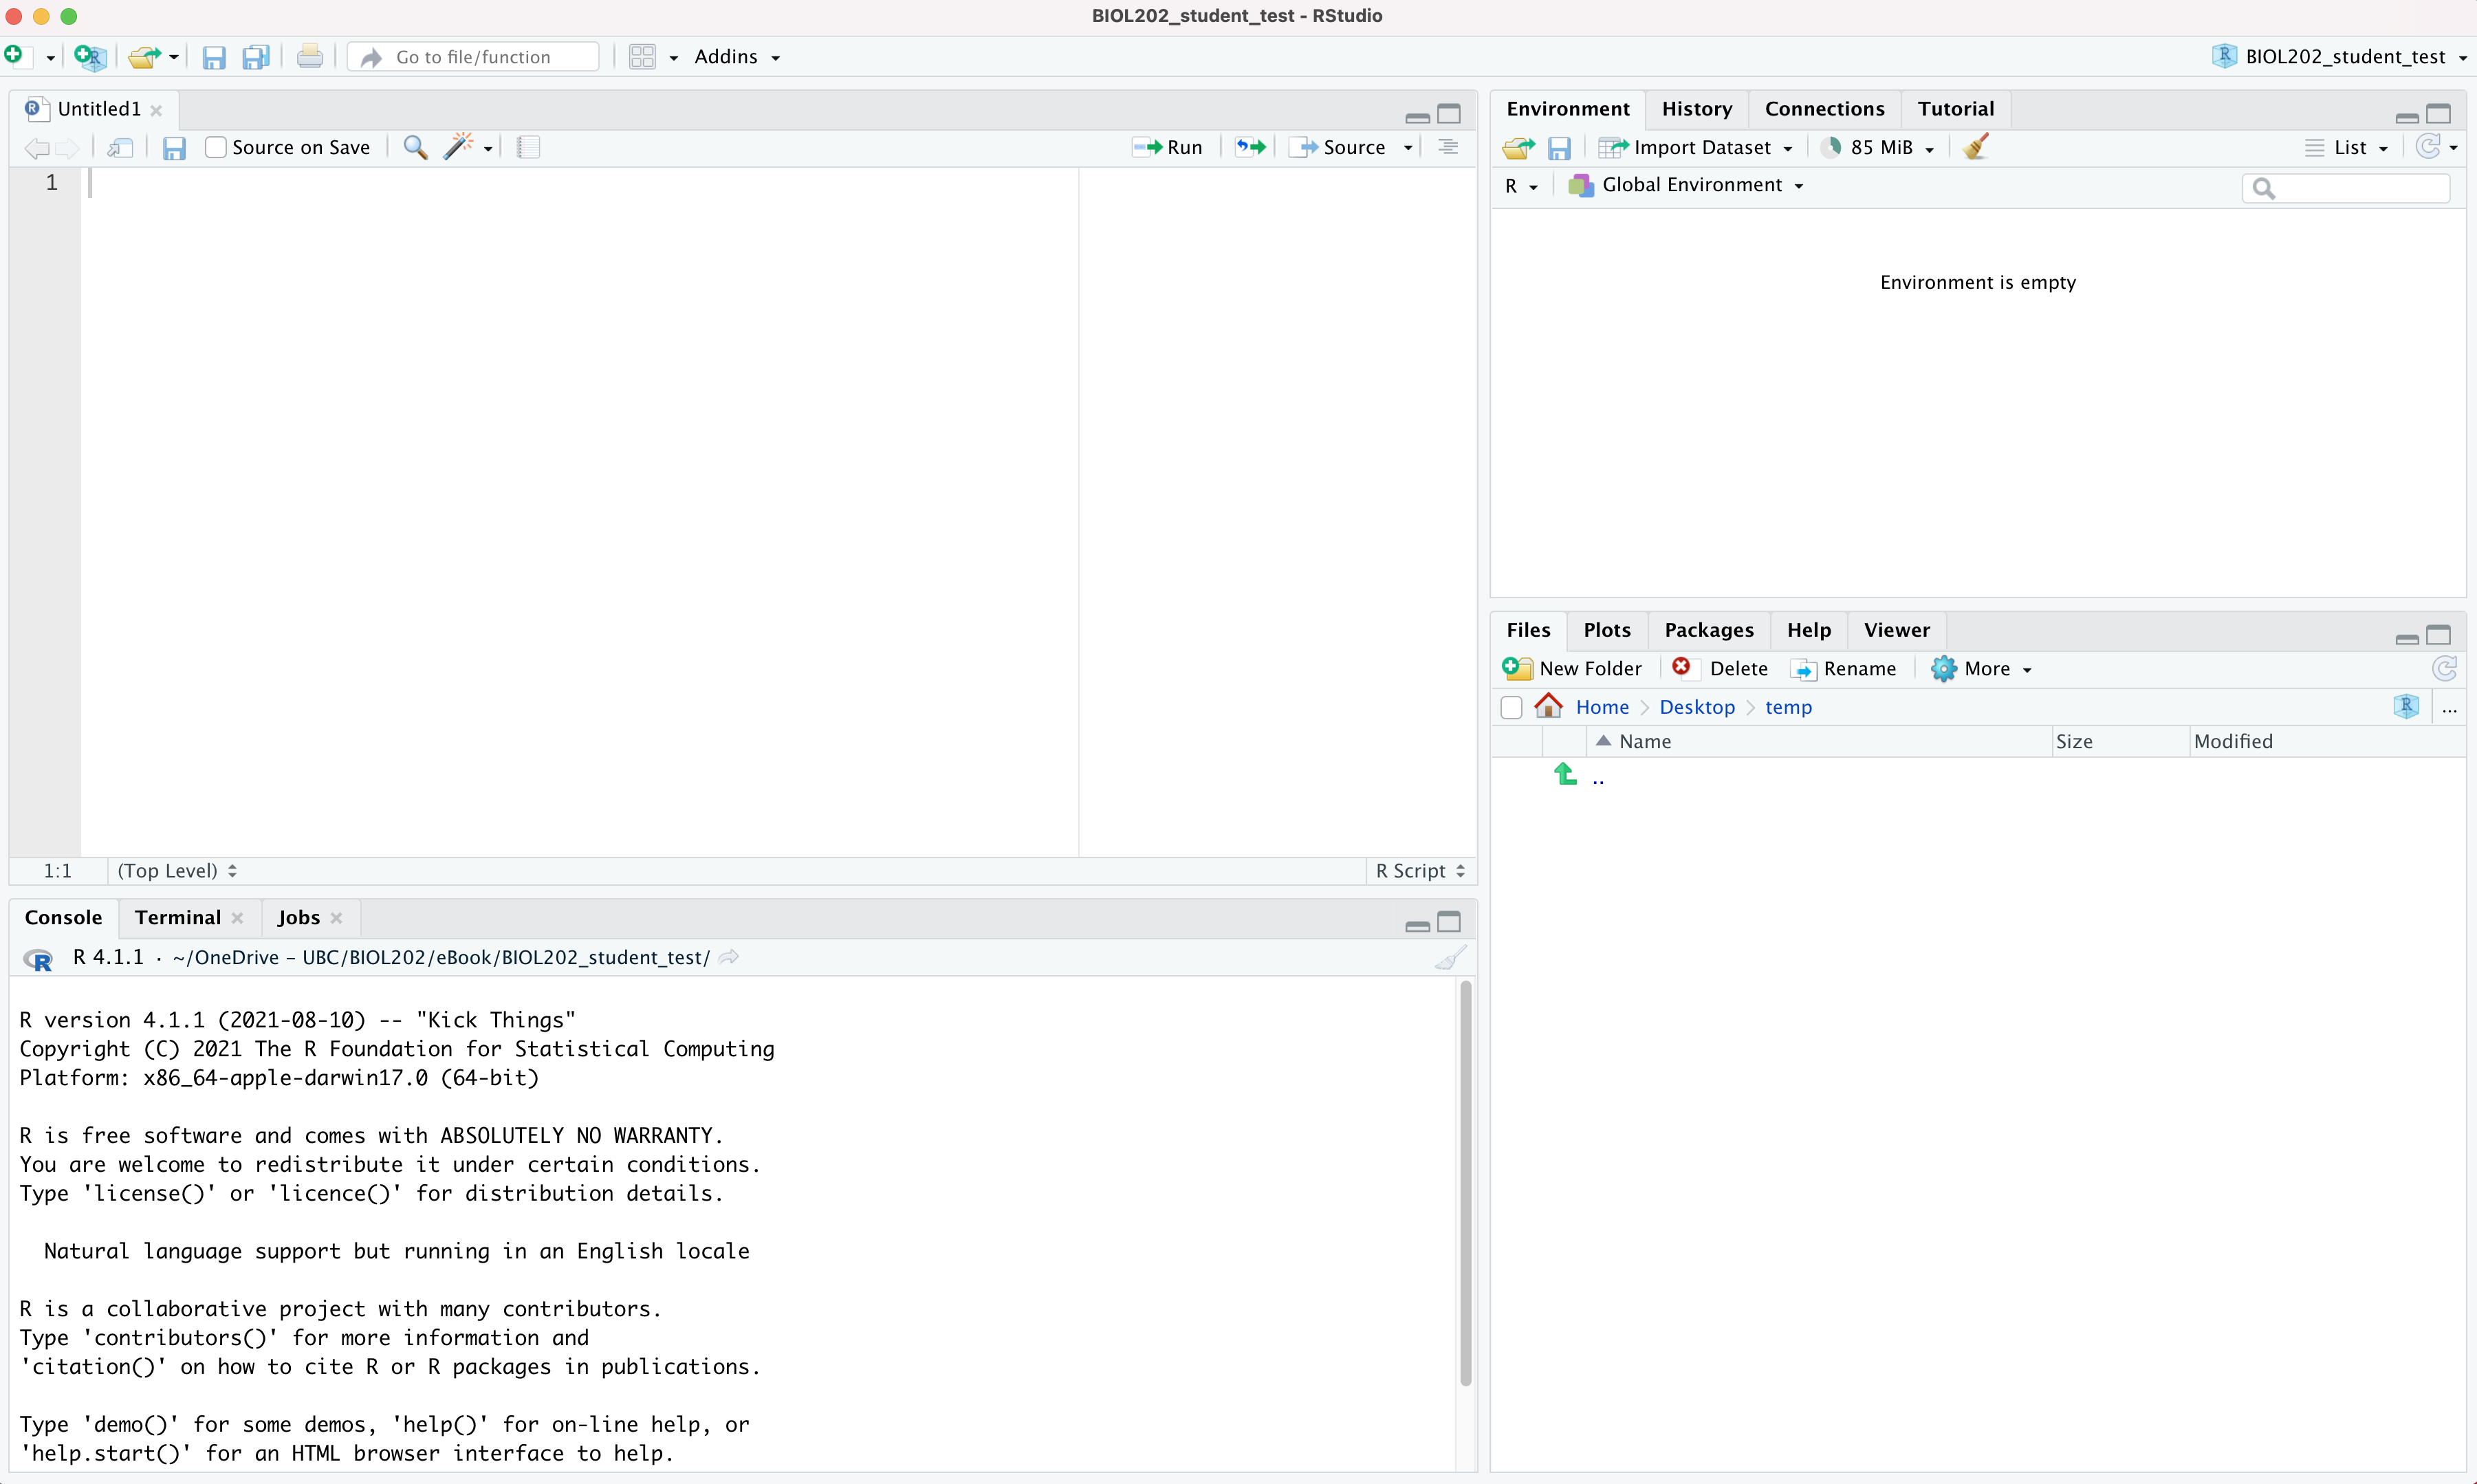
\includegraphics{./more/RStudio_Window.png}

Note the four panes which are four panels dividing the screen: the source pane (top left), console pane (bottom left), the files pane (bottom right), and the environment pane (top right). Over the course of this chapter, you'll come to learn what purpose each of these panes serves.

\section{Coding basics}\label{coding_basics}

Please go through section \href{https://moderndive.com/1-getting-started.html\#code}{1.2 of the ModernDive online text} called ``How do I code in R?''. This should take about \textbf{15 minutes}.

You may get overwhelmed by all the terminology on that page\ldots{} don't worry! You can simply bookmark that page for future reference. But it does cover the coding basics very well!

\section{R packages}\label{packages}

An R package is a collection of functions, data, and documentation that extends the capabilities of R. They are written by a world-wide community of R users. For example, among the most popular packages are:

\begin{itemize}
\tightlist
\item
  \texttt{ggplot2} package for data visualization
\item
  \texttt{dplyr} package for data wrangling
\item
  \texttt{tidyverse}, which is a package that includes a collection of multiple packages (including the preceding two) that are all installed at once. We'll be using this package in the course.
\end{itemize}

There are two key things to remember about R packages:

\begin{itemize}
\item
  \emph{Installation}: Most packages are not installed by default when you install R and RStudio. You need to install a package before you can use it. Once you've installed it, you likely don't need to install it again unless you want to update it to a newer version of the package.
\item
  \emph{Loading}: Packages are not loaded automatically when you open RStudio. You need to load them everytime you open RStudio.
\end{itemize}

\section{Package installation}\label{package_install}

Let's install the \texttt{tidyverse} package.

There are two ways to install an R package:

\begin{itemize}
\tightlist
\item
  In the Files pane:

  \begin{itemize}
  \tightlist
  \item
    Click on ``Packages''
  \item
    Click on ``Install''
  \item
    Type the name of the package under ``Packages (separate multiple with space or comma):'' In this case, type \texttt{tidyverse}
  \item
    Click ``Install''
  \end{itemize}
\item
  Alternatively, in the Console pane type the following
\end{itemize}

Later, when you start using R Markdown, never include the following ``install.packages'' code within your R Markdown document; only install packages by typing directly in the Console!

\begin{Shaded}
\begin{Highlighting}[]
\FunctionTok{install.packages}\NormalTok{(}\StringTok{"tidyverse"}\NormalTok{)}
\end{Highlighting}
\end{Shaded}

If you are attempting to install a package (using \texttt{install.packages}) and you get this message:

\begin{verbatim}
There is a binary version available but the source version is later:
  binary source needs_compilation
systemfonts  1.0.2  1.0.3              TRUE

Do you want to install from sources the package which needs compilation? (Yes/no/cancel)
\end{verbatim}

Respond with ``no'' (without quotes). Do NOT respond ``Yes''.

When working on your own computer, you only need to install a package once, unless you want to update an already installed package to the latest version (something you might do every 6 months or so). \textbf{HOWEVER}: If you're working on a school computer (in a computer lab or in the library), you may need to install packages each session, because local files (on the computer) are automatically deleted daily. If you're unsure what packages are already installed, consult the ``packages'' tab in the lower-right RStudio pane when you start up RStudio; installed packages are listed there.

\section{Package loading}\label{package_load}

Let's load the \texttt{tidyverse} package.

After you've installed a package, you can now load it using the \texttt{library()} command. For example, to load the \texttt{tidyverse} package, run the following code in the Console pane:

\begin{Shaded}
\begin{Highlighting}[]
\FunctionTok{library}\NormalTok{(tidyverse)}
\end{Highlighting}
\end{Shaded}

You have to reload each package you want to use every time you open a new session of RStudio. This is a little annoying to get used to and will be your most common error as you begin. When you see an error such as

\begin{verbatim}
Error: could not find function
\end{verbatim}

remember that this likely comes from you trying to use a function in a package that has not been loaded. Remember to run the \texttt{library()} function with the appropriate package to fix this error.

\section{Intro to R Markdown}\label{intro_markdown}

As you may have learned already from relevant section in the \href{https://ubco-biology.github.io/Procedures-and-Guidelines/markdown-1.html}{Biology Procedures and Guidelines resource}, R Markdown is a markup language that provides an easy way to produce a rich, fully-documented reproducible analysis. It allows its user to share a single file that contains all of the commentary, R code, and metadata needed to reproduce the analysis from beginning to end. R Markdown allows for ``chunks'' of R code to be included along with Markdown text to produce a nicely formatted HTML, PDF, or Word file without having to know any complicated programming languages or having to fuss with getting the formatting just right in a Microsoft Word DOCX file.

One R Markdown file can generate a variety of different formats and all of this is done in a single text file with a few bits of formatting. You'll be pleasantly surprised at how easy it is to write an R Markdown document after your first few attempts.

We will be using R Markdown to create reproducible lab reports.

R Markdown is just one flavour of a markup language. RStudio can be used to edit R Markdown. There are many other markdown editors out there, but using RStudio is good for our purposes.

\section{Literate programming with R Markdown}\label{lit_programming}

\begin{enumerate}
\def\labelenumi{\arabic{enumi}.}
\tightlist
\item
  View the following short video:
\end{enumerate}

\href{https://youtu.be/lNWVQ2oxNho}{\textbf{Why use R Markdown for Lab Reports?}}

The preceding video described what can be referred to as \textbf{literate programming}: authoring a single document that integrates data analysis (executable code) with textual documentation, linking data, code, and text. In R Markdown, the executable R code is placed in ``chunks'', and these are embedded throughout sections of regular text.

For an example of a PDF document that illustrates literate programming, see \href{https://osf.io/59j4b}{here}. It accompanied a lab-based experiment examining the potential for freshwater diatoms to be successfully dispersed over long distances adhered to duck feathers.

\begin{enumerate}
\def\labelenumi{\arabic{enumi}.}
\setcounter{enumi}{1}
\tightlist
\item
  View the following \href{https://www.youtube.com/watch?v=asHhuHRxhvo}{youtube video} on creating an R Markdown document.
\end{enumerate}

If you'd like additional introductory tutorials on R Markdown, see this \href{https://rmarkdown.rstudio.com/lesson-1.html}{one from RStudio}, or this \href{https://rbasics.netlify.app/4-rmarkdown.html}{one}.

\section{Making sure R Markdown knits to PDF}\label{veryify_knit}

Now we're going to ensure R Markdown works the way we want. A key functionality we need is being able to ``knit'' our report to PDF format.

With the newest versions of RStudio, you may be able to knit to PDF without doing anything special first.

Let's give this a try:

Step 1: While in RStudio, select the ``+'' dropdown icon at top left of RStudio window, and select R Markdown. RStudio may at this point install a bunch of things, and if so that's ok. It may also ask you to install the \texttt{rmarkdown} package.. if it does, do so!

Step 2: A window will then appear and you can replace the ``Untitled'' with something like ``Test'', then select OK.

Step 3: This will open an R Markdown document in the top left panel. Don't worry about all the text in there at this point. What we want to do is test whether it will ``knit'' (render) the document to PDF format.

Step 4: Select the ``Knit'' drop-down icon at the top of the RStudio window, and select ``Knit to PDF''. RStudio will ask you to first save the markdown file (save it anywhere with any name for now), then it will process the markdown file and render it to PDF.

If this worked, great!! You can ignore the next section here. If it didn't work, then proceed to this next section:

If the preceding steps did not result in you being able to knit your markdown document to PDF, then do this:

Install the \texttt{tinytex} package by typing this code into the command console of RStudio:

\begin{verbatim}
install.packages("tinytex")
\end{verbatim}

Then, once that has installed successfully, type the following:

\begin{verbatim}
tinytex::install_tinytex()
\end{verbatim}

RStudio will take a minute or two to install a bunch of things. Once it's done, we're ready to try knitting to PDF.

Recall you only need to install a package once! And this should be the last time you need to deal with the \texttt{tinytex} package (you won't need to ``load'' it in future), because now that it's installed, its functionality works in the background with RStudio.

Now go back to the steps 1 through 4 above to try knitting your markdown document to PDF.

In a future \hyperref[repro_research]{tutorial} we'll discuss how to use R Markdown as part of a reproducible workflow.

\section{Extra resources}\label{r_resources}

This page is still under development (Aug 2022)

If you are googling for R code, make sure to also include package names in your search query (if you are using a specific package). For example, instead of googling ``scatterplot in R'', google ``scatterplot in R with ggplot2''.

Rstudio provides links to several \textbf{cheatsheets} that will come in handy throughout the semester.

You can get nice PDF versions of the files by going to \textbf{Help -\textgreater{} Cheatsheets} inside RStudio:

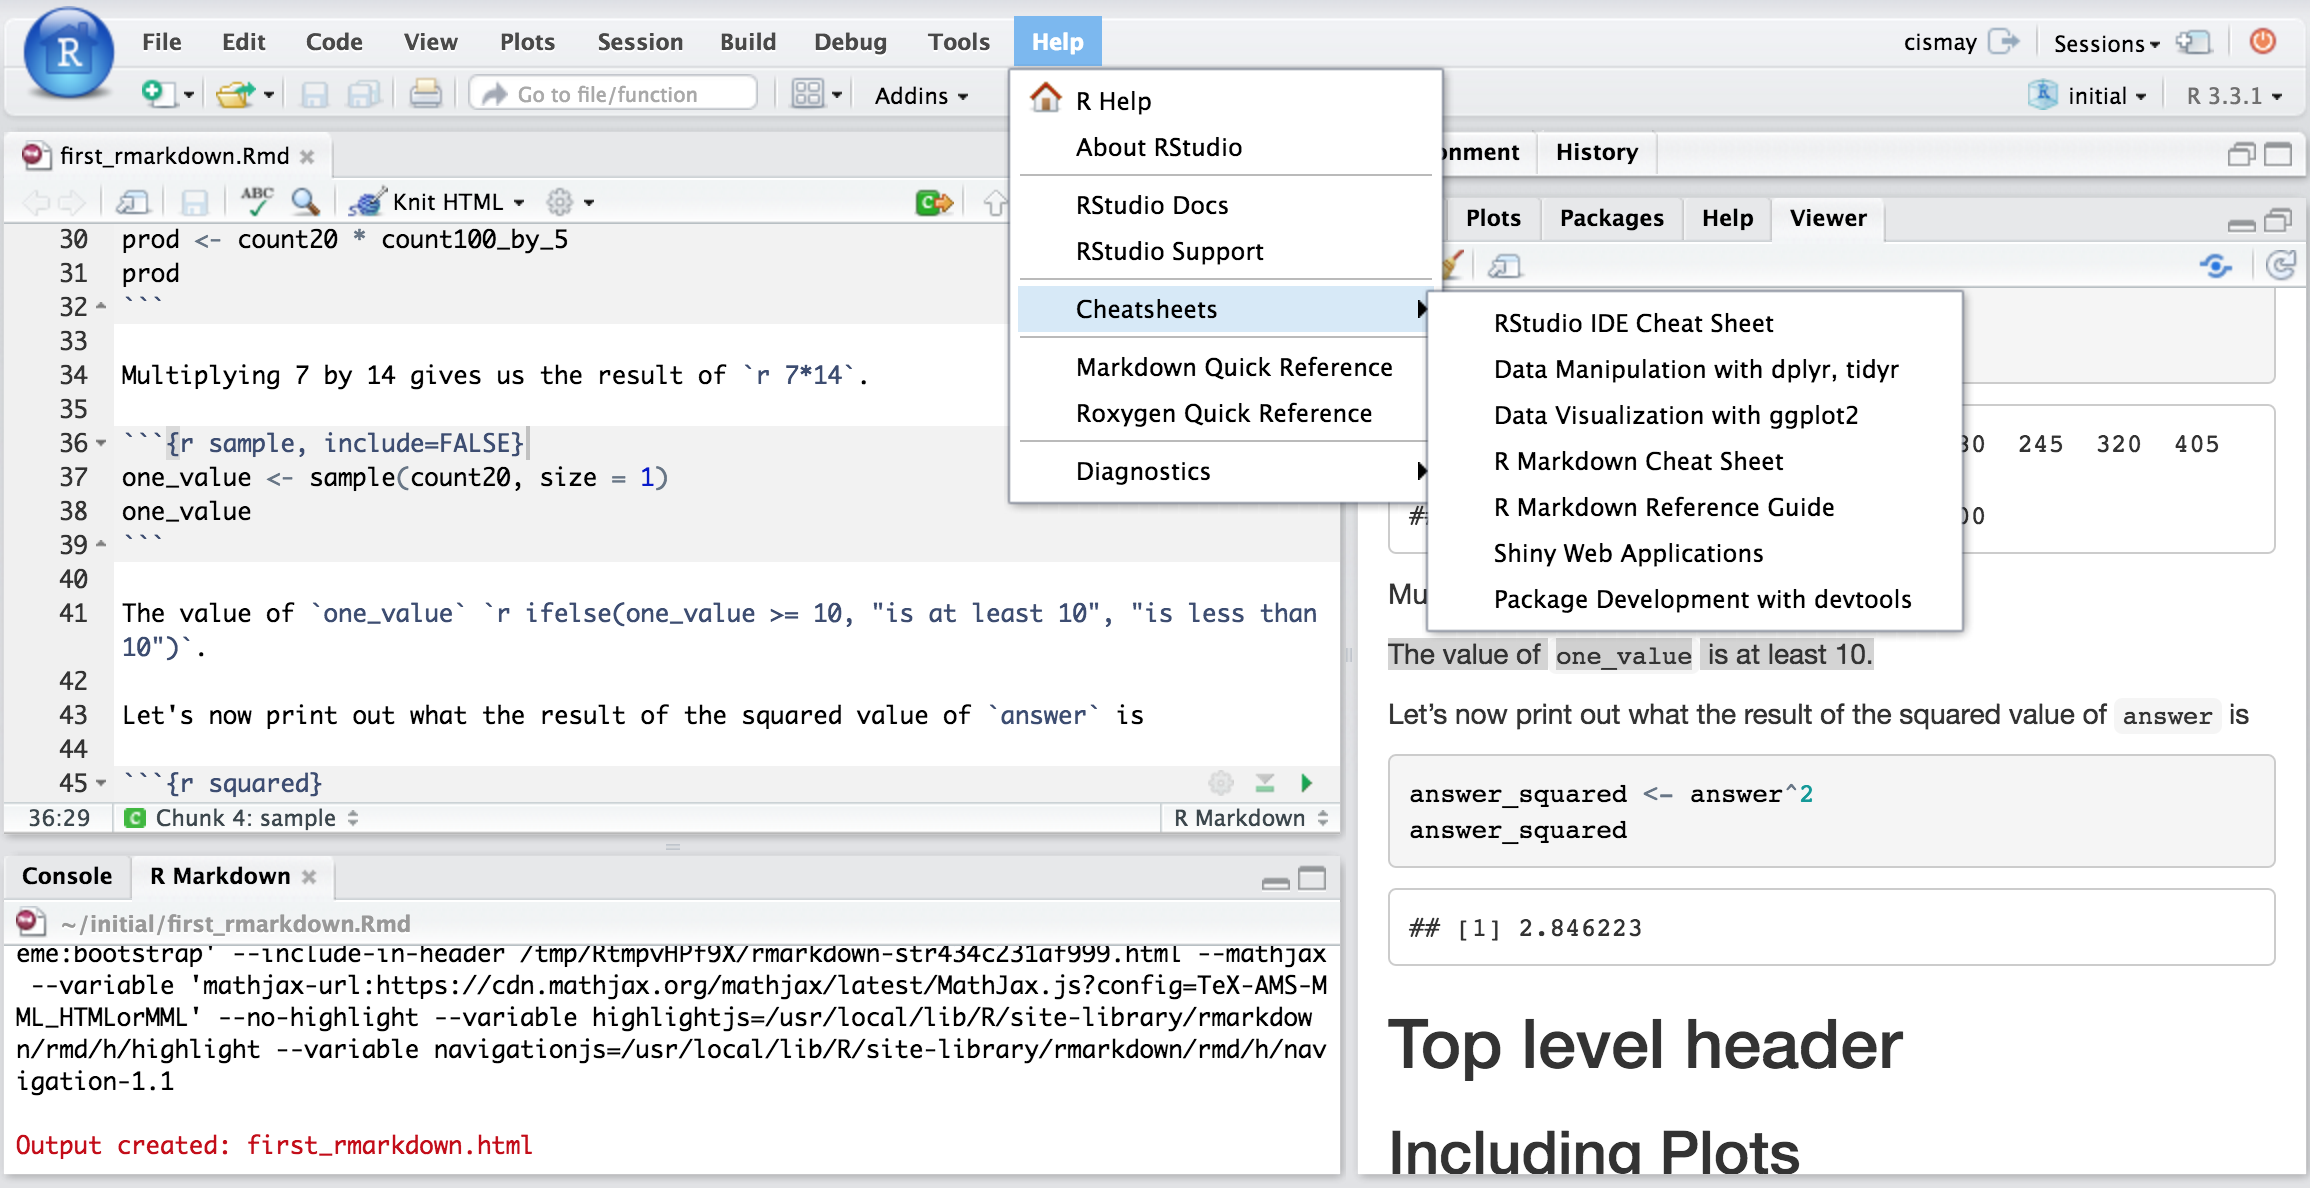
\includegraphics{./more/cheatsheets.png}

The book titled ``Getting used to R, RStudio, and R Markdown'' by Chester Ismay, which can be freely accessed \href{https://ismayc.github.io/rbasics-book/}{here}, is also a wonderful resource for for new users of R, RStudio, and R Markdown. It includes examples showing working with R Markdown files in RStudio recorded as GIFs.

\section{R Resources Online}\label{online_resources}

\begin{longtable}[]{@{}
  >{\raggedright\arraybackslash}p{(\columnwidth - 2\tabcolsep) * \real{0.6667}}
  >{\raggedright\arraybackslash}p{(\columnwidth - 2\tabcolsep) * \real{0.3333}}@{}}
\caption{Learning R - Tutorials and workshop materials}\tabularnewline
\toprule\noalign{}
\begin{minipage}[b]{\linewidth}\raggedright
URL
\end{minipage} & \begin{minipage}[b]{\linewidth}\raggedright
Purpose
\end{minipage} \\
\midrule\noalign{}
\endfirsthead
\toprule\noalign{}
\begin{minipage}[b]{\linewidth}\raggedright
URL
\end{minipage} & \begin{minipage}[b]{\linewidth}\raggedright
Purpose
\end{minipage} \\
\midrule\noalign{}
\endhead
\bottomrule\noalign{}
\endlastfoot
\url{https://whitlockschluter3e.zoology.ubc.ca}. & R resources to accompany Whitlock \& Schluter text \\
\url{https://datacarpentry.org/R-genomics/01-intro-to-R.htm} & l Data Carpentry Intro R tutorials \\
\url{https://r-dir.com/learn/tutorials.html} & List of useful tutorials including videos \\
\url{https://www.rstudio.com/resources/webinars/} & Various online learning materials at RStudio \\
\url{https://rmd4sci.njtierney.com} & R Markdown for Scientists \\
\url{http://r4ds.had.co.nz/index.html} & Hadley Wickham's online book \\
\end{longtable}

\begin{center}\rule{0.5\linewidth}{0.5pt}\end{center}

\begin{longtable}[]{@{}
  >{\raggedright\arraybackslash}p{(\columnwidth - 2\tabcolsep) * \real{0.6667}}
  >{\raggedright\arraybackslash}p{(\columnwidth - 2\tabcolsep) * \real{0.3333}}@{}}
\caption{So many packages - how to find useful ones?}\tabularnewline
\toprule\noalign{}
\begin{minipage}[b]{\linewidth}\raggedright
URL
\end{minipage} & \begin{minipage}[b]{\linewidth}\raggedright
Purpose
\end{minipage} \\
\midrule\noalign{}
\endfirsthead
\toprule\noalign{}
\begin{minipage}[b]{\linewidth}\raggedright
URL
\end{minipage} & \begin{minipage}[b]{\linewidth}\raggedright
Purpose
\end{minipage} \\
\midrule\noalign{}
\endhead
\bottomrule\noalign{}
\endlastfoot
\url{http://blog.revolutionanalytics.com/beginner-tips/} & Beginner tips \\
& \\
\url{https://mran.microsoft.com/packages/} & Tool for exploring packages \\
\end{longtable}

\begin{center}\rule{0.5\linewidth}{0.5pt}\end{center}

\begin{longtable}[]{@{}
  >{\raggedright\arraybackslash}p{(\columnwidth - 2\tabcolsep) * \real{0.6806}}
  >{\raggedright\arraybackslash}p{(\columnwidth - 2\tabcolsep) * \real{0.3194}}@{}}
\caption{Data analysis in R}\tabularnewline
\toprule\noalign{}
\begin{minipage}[b]{\linewidth}\raggedright
URL
\end{minipage} & \begin{minipage}[b]{\linewidth}\raggedright
Purpose
\end{minipage} \\
\midrule\noalign{}
\endfirsthead
\toprule\noalign{}
\begin{minipage}[b]{\linewidth}\raggedright
URL
\end{minipage} & \begin{minipage}[b]{\linewidth}\raggedright
Purpose
\end{minipage} \\
\midrule\noalign{}
\endhead
\bottomrule\noalign{}
\endlastfoot
\url{https://www.zoology.ubc.ca/~schluter/R/} & UBC zoology site handy stats reference \\
\url{http://statmethods.net/} & Good general reference \\
\end{longtable}

\begin{center}\rule{0.5\linewidth}{0.5pt}\end{center}

\begin{longtable}[]{@{}
  >{\raggedright\arraybackslash}p{(\columnwidth - 2\tabcolsep) * \real{0.6806}}
  >{\raggedright\arraybackslash}p{(\columnwidth - 2\tabcolsep) * \real{0.3194}}@{}}
\caption{Data visualization in R}\tabularnewline
\toprule\noalign{}
\begin{minipage}[b]{\linewidth}\raggedright
URL
\end{minipage} & \begin{minipage}[b]{\linewidth}\raggedright
Purpose
\end{minipage} \\
\midrule\noalign{}
\endfirsthead
\toprule\noalign{}
\begin{minipage}[b]{\linewidth}\raggedright
URL
\end{minipage} & \begin{minipage}[b]{\linewidth}\raggedright
Purpose
\end{minipage} \\
\midrule\noalign{}
\endhead
\bottomrule\noalign{}
\endlastfoot
\url{http://statmethods.net/} & Good general reference for graphing \\
\url{http://ggplot2.org/book/} & Hadley Wickhams's ggplot2 book online \\
\url{http://stats.idre.ucla.edu/r/seminars/ggplot2_intro/} & Great tutorial on ggplot2 \\
\url{http://www.cookbook-r.com/Graphs/} & Graphing with ggplot2 \\
\end{longtable}

\begin{center}\rule{0.5\linewidth}{0.5pt}\end{center}

\begin{longtable}[]{@{}ll@{}}
\caption{BLOGs and general resources}\tabularnewline
\toprule\noalign{}
URL & Purpose \\
\midrule\noalign{}
\endfirsthead
\toprule\noalign{}
URL & Purpose \\
\midrule\noalign{}
\endhead
\bottomrule\noalign{}
\endlastfoot
\url{https://www.r-bloggers.com/} & Popular blog site, lots of info \\
\url{http://rseek.org/} & Search engine for R help \\
\end{longtable}

\begin{center}\rule{0.5\linewidth}{0.5pt}\end{center}

\begin{longtable}[]{@{}
  >{\raggedright\arraybackslash}p{(\columnwidth - 2\tabcolsep) * \real{0.7778}}
  >{\raggedright\arraybackslash}p{(\columnwidth - 2\tabcolsep) * \real{0.2222}}@{}}
\caption{Resources for reproducible research / open science}\tabularnewline
\toprule\noalign{}
\begin{minipage}[b]{\linewidth}\raggedright
URL
\end{minipage} & \begin{minipage}[b]{\linewidth}\raggedright
Purpose
\end{minipage} \\
\midrule\noalign{}
\endfirsthead
\toprule\noalign{}
\begin{minipage}[b]{\linewidth}\raggedright
URL
\end{minipage} & \begin{minipage}[b]{\linewidth}\raggedright
Purpose
\end{minipage} \\
\midrule\noalign{}
\endhead
\bottomrule\noalign{}
\endlastfoot
\url{https://cos.io/} & Center for Open Science \\
\url{https://ropensci.org/} & Open science R resources \\
\url{http://geoscripting-wur.github.io/RProjectManagement/} & Lessons about version control \\
\url{https://nicercode.github.io/} & Helping to improve your code \\
\end{longtable}

\begin{center}\rule{0.5\linewidth}{0.5pt}\end{center}

\begin{longtable}[]{@{}
  >{\raggedright\arraybackslash}p{(\columnwidth - 2\tabcolsep) * \real{0.7808}}
  >{\raggedright\arraybackslash}p{(\columnwidth - 2\tabcolsep) * \real{0.2192}}@{}}
\caption{Geospatial work in R}\tabularnewline
\toprule\noalign{}
\begin{minipage}[b]{\linewidth}\raggedright
URL
\end{minipage} & \begin{minipage}[b]{\linewidth}\raggedright
Purpose
\end{minipage} \\
\midrule\noalign{}
\endfirsthead
\toprule\noalign{}
\begin{minipage}[b]{\linewidth}\raggedright
URL
\end{minipage} & \begin{minipage}[b]{\linewidth}\raggedright
Purpose
\end{minipage} \\
\midrule\noalign{}
\endhead
\bottomrule\noalign{}
\endlastfoot
\url{http://spatial.ly/r/} & Example maps with R \\
\url{https://rstudio.github.io/leaflet/} & Online mapping with R \\
\url{https://www.earthdatascience.org/courses/earth-analytics/} & Excellent course \\
& \\
\url{https://geoscripting-wur.github.io/} & Amazing ``geoscripting'' tutorial \\
\end{longtable}

\part*{Reproducible Workflows}\label{part-reproducible-workflows}
\addcontentsline{toc}{part}{Reproducible Workflows}

\chapter{Reproducible Research}\label{repro_research}

A key goal of our Biology program at UBC's Okanagan campus is to foster appreciation for reproducible research, and to equip students (and professors) with skills that will help them undertake reproducible research themselves.

In first year you learned from the Biology program's \href{https://ubco-biology.github.io/OS-Introduction/}{introductory Open Science learning modules} that reproducible research studies are not as common as one might assume. One key reason for this is insufficient documentation of all the steps taken along the research workflow. Moreover, conducting reproducible research is extremely challenging - more than most scientists appreciate. See, for example, an incredible, recent case concerning ageing experiments with \emph{C. elegans} \href{https://www.nature.com/news/a-long-journey-to-reproducible-results-1.22478}{here}.

In the BIOL202 lectures you'll learn more about the various causes of irreproducible research, and about the practices that can help promote reproducibility. In this lab component of the course, you'll learn the basics of how to achieve an acceptable level of \emph{computational reproducibility} (complete computational reproducibility is actually pretty tricky, but we'll get close).

\section{Computational reproducibility}\label{comp_repro}

Almost all research, whether it's conducted in the field or in a lab, includes a substantial amount of work that's done on the computer. This includes data processing, statistical analyses, data visualization and presentation, and production of research outputs (e.g.~publications). Some research is of course exclusively conducted on computers. The bottom line is that computer-based work forms a key and substantive part of all research workflows.

Given that this work is done on computers (which are entirely controllable), it should be able to be reproduced \textbf{exactly}. This is known as \textbf{computational reproducibility}: an independent researcher should be able to access all data and scripts from a study, run those scripts, and get exactly the same outputs and results as reported in the original study.

In this tutorial you'll start gaining relevant experience and skills by producing a reproducible lab report.

A \emph{workflow} refers to the the steps you take when conducting your day-to-day work - say, on a term project, for example. Having a well-designed workflow improves efficiency, and when done right, reproducibility. It includes, for example, how you create, access, and manage files on your computer (or in the cloud).

Following best practices for naming and organizing your files and directories on your computer will help ensure that you can spend more time doing the important work, and less time fiddling and trying to remember what you did and where you saved your work. It will also help your future self, when labs and assignments in upper year courses request that you use R and R Markdown for analyses and reports.

\begin{enumerate}
\def\labelenumi{\arabic{enumi}.}
\tightlist
\item
  Review the Biology department's \href{https://ubco-biology.github.io/Procedures-and-Guidelines/}{Procedures and Guidelines webpage} description of how to \href{https://ubco-biology.github.io/Procedures-and-Guidelines/file-and-data-management.html}{manage files and directories}. This should take about \textbf{20 minutes}
\end{enumerate}

\section{An example BIOL202 workflow}\label{biol202_workflow}

Now that you have reviewed the fundamentals of file and directory management, you should decide how to best organize and manage the work you do for BIOL202. Here we'll provide one example approach that most if not all of you will find useful.

\section{Microsoft OneDrive}\label{onedrive}

Our suggested approach assumes you have set up a Microsoft account through UBC (using your CWL), and have set up the OneDrive application on your own computer, which automatically syncs (when you're online) selected files/directories between your local computer and your OneDrive account in the cloud.

Why OneDrive? As a UBC student, you receive 1TB of free storage! And you also get peace of mind knowing that your files are secure and up-to-date (provided you have an internet connection), and that OneDrive has something called ``version control'', which saves old versions of files and allows you to see those versions if you wish, \textbf{so long as you maintain the same file name}.

\textbf{WAIT A SECOND!} In the \href{https://ubco-biology.github.io/Procedures-and-Guidelines/file-naming.html}{``File Naming''} instructions that I just reviewed, I was instructed to create a new file with a new version number in the filename (e.g.~with a ``V0'', ``V1'', ``V2'' etc\ldots) each time I worked on it!

Those instructions are entirely valid! However, when you have access to a \emph{version control} system, like OneDrive, it is better to \textbf{keep the file name the same}, rather than changing it each time you update it. For example, your markdown file (which as a ``.Rmd'' extension to the name) that you use for your tutorial work should maintain the same name throughout the term, rather than saving a new file each time you do substantive work on it.

Assuming your files are syncing properly between your computer and OneDrive (and this simply requires that you're connected to the internet), you will always be able to \href{https://support.microsoft.com/en-us/office/restore-a-previous-version-of-a-file-stored-in-onedrive-159cad6d-d76e-4981-88ef-de6e96c93893}{see (and if desired, restore) old versions of your files}.

If you haven't set up OneDrive yet, follow the instructions provided at this \href{https://lthub.ubc.ca/guides/microsoft-onedrive-student-guide/}{UBC IT website}.

Using OneDrive is entirely optional. If you choose not to use OneDrive, please follow the file naming instructions from the \href{https://ubco-biology.github.io/Procedures-and-Guidelines/file-naming.html}{Procedures and Guidelines document}. And you can still follow the directory structure instructions below, regardless of where you set up your directories (OneDrive or not).

\section{Directory structure}\label{dir_structure}

We anticipate three general categories of work being undertaken:

\begin{itemize}
\tightlist
\item
  Lecture work, including annotating lecture notes (e.g.~on PDFs or PowerPoints) and writing study notes of your own (e.g.~using Word)
\item
  Tutorial work, including practicing what you learn in tutorials using RStudio and R Markdown, and commenting about tips, or tricky bits
\item
  Lab assignment work, in which you answer questions using R and R Markdown and create a document for submission and grading
\end{itemize}

Each of these categories of work should have their own directory, and all three of these directories should exist within a ``root'' directory called ``BIOL202''.

\section{Steps to set up directories}\label{setup_dirs}

\begin{itemize}
\tightlist
\item
  Having successfully installed OneDrive, you should see a ``OneDrive'' folder on your computer
\item
  In your OneDrive folder, create a root directory ``BIOL202'' to host all of your BIOL202 work
\item
  Create a ``\_README.txt file for the root BIOL202 directory, as per instructions in the \href{https://ubco-biology.github.io/Procedures-and-Guidelines/readme-files-and-data-dictionaries.html}{Biology Procedures and Guidelines webpage}.
\end{itemize}

You can create and edit your ``\_README.txt'' file in RStudio! Just click on the ``+'' drop down at the top left, and select ``Text file''. Then type in the information you need, and name it ``\_README.txt'' and save it in the appropriate directory.

\begin{itemize}
\tightlist
\item
  Within the BIOL202 root directory, create three (sub)directories:

  \begin{itemize}
  \tightlist
  \item
    ``BIOL202\_lecture''
  \item
    ``BIOL202\_tutorials''
  \item
    ``BIOL202\_assignments''
  \end{itemize}
\item
  Create a ``\_README.txt'' file in each of the three sub-directories (again, you can use RStudio to create these!).
\end{itemize}

An example setup is illustrated below.

\begin{figure}
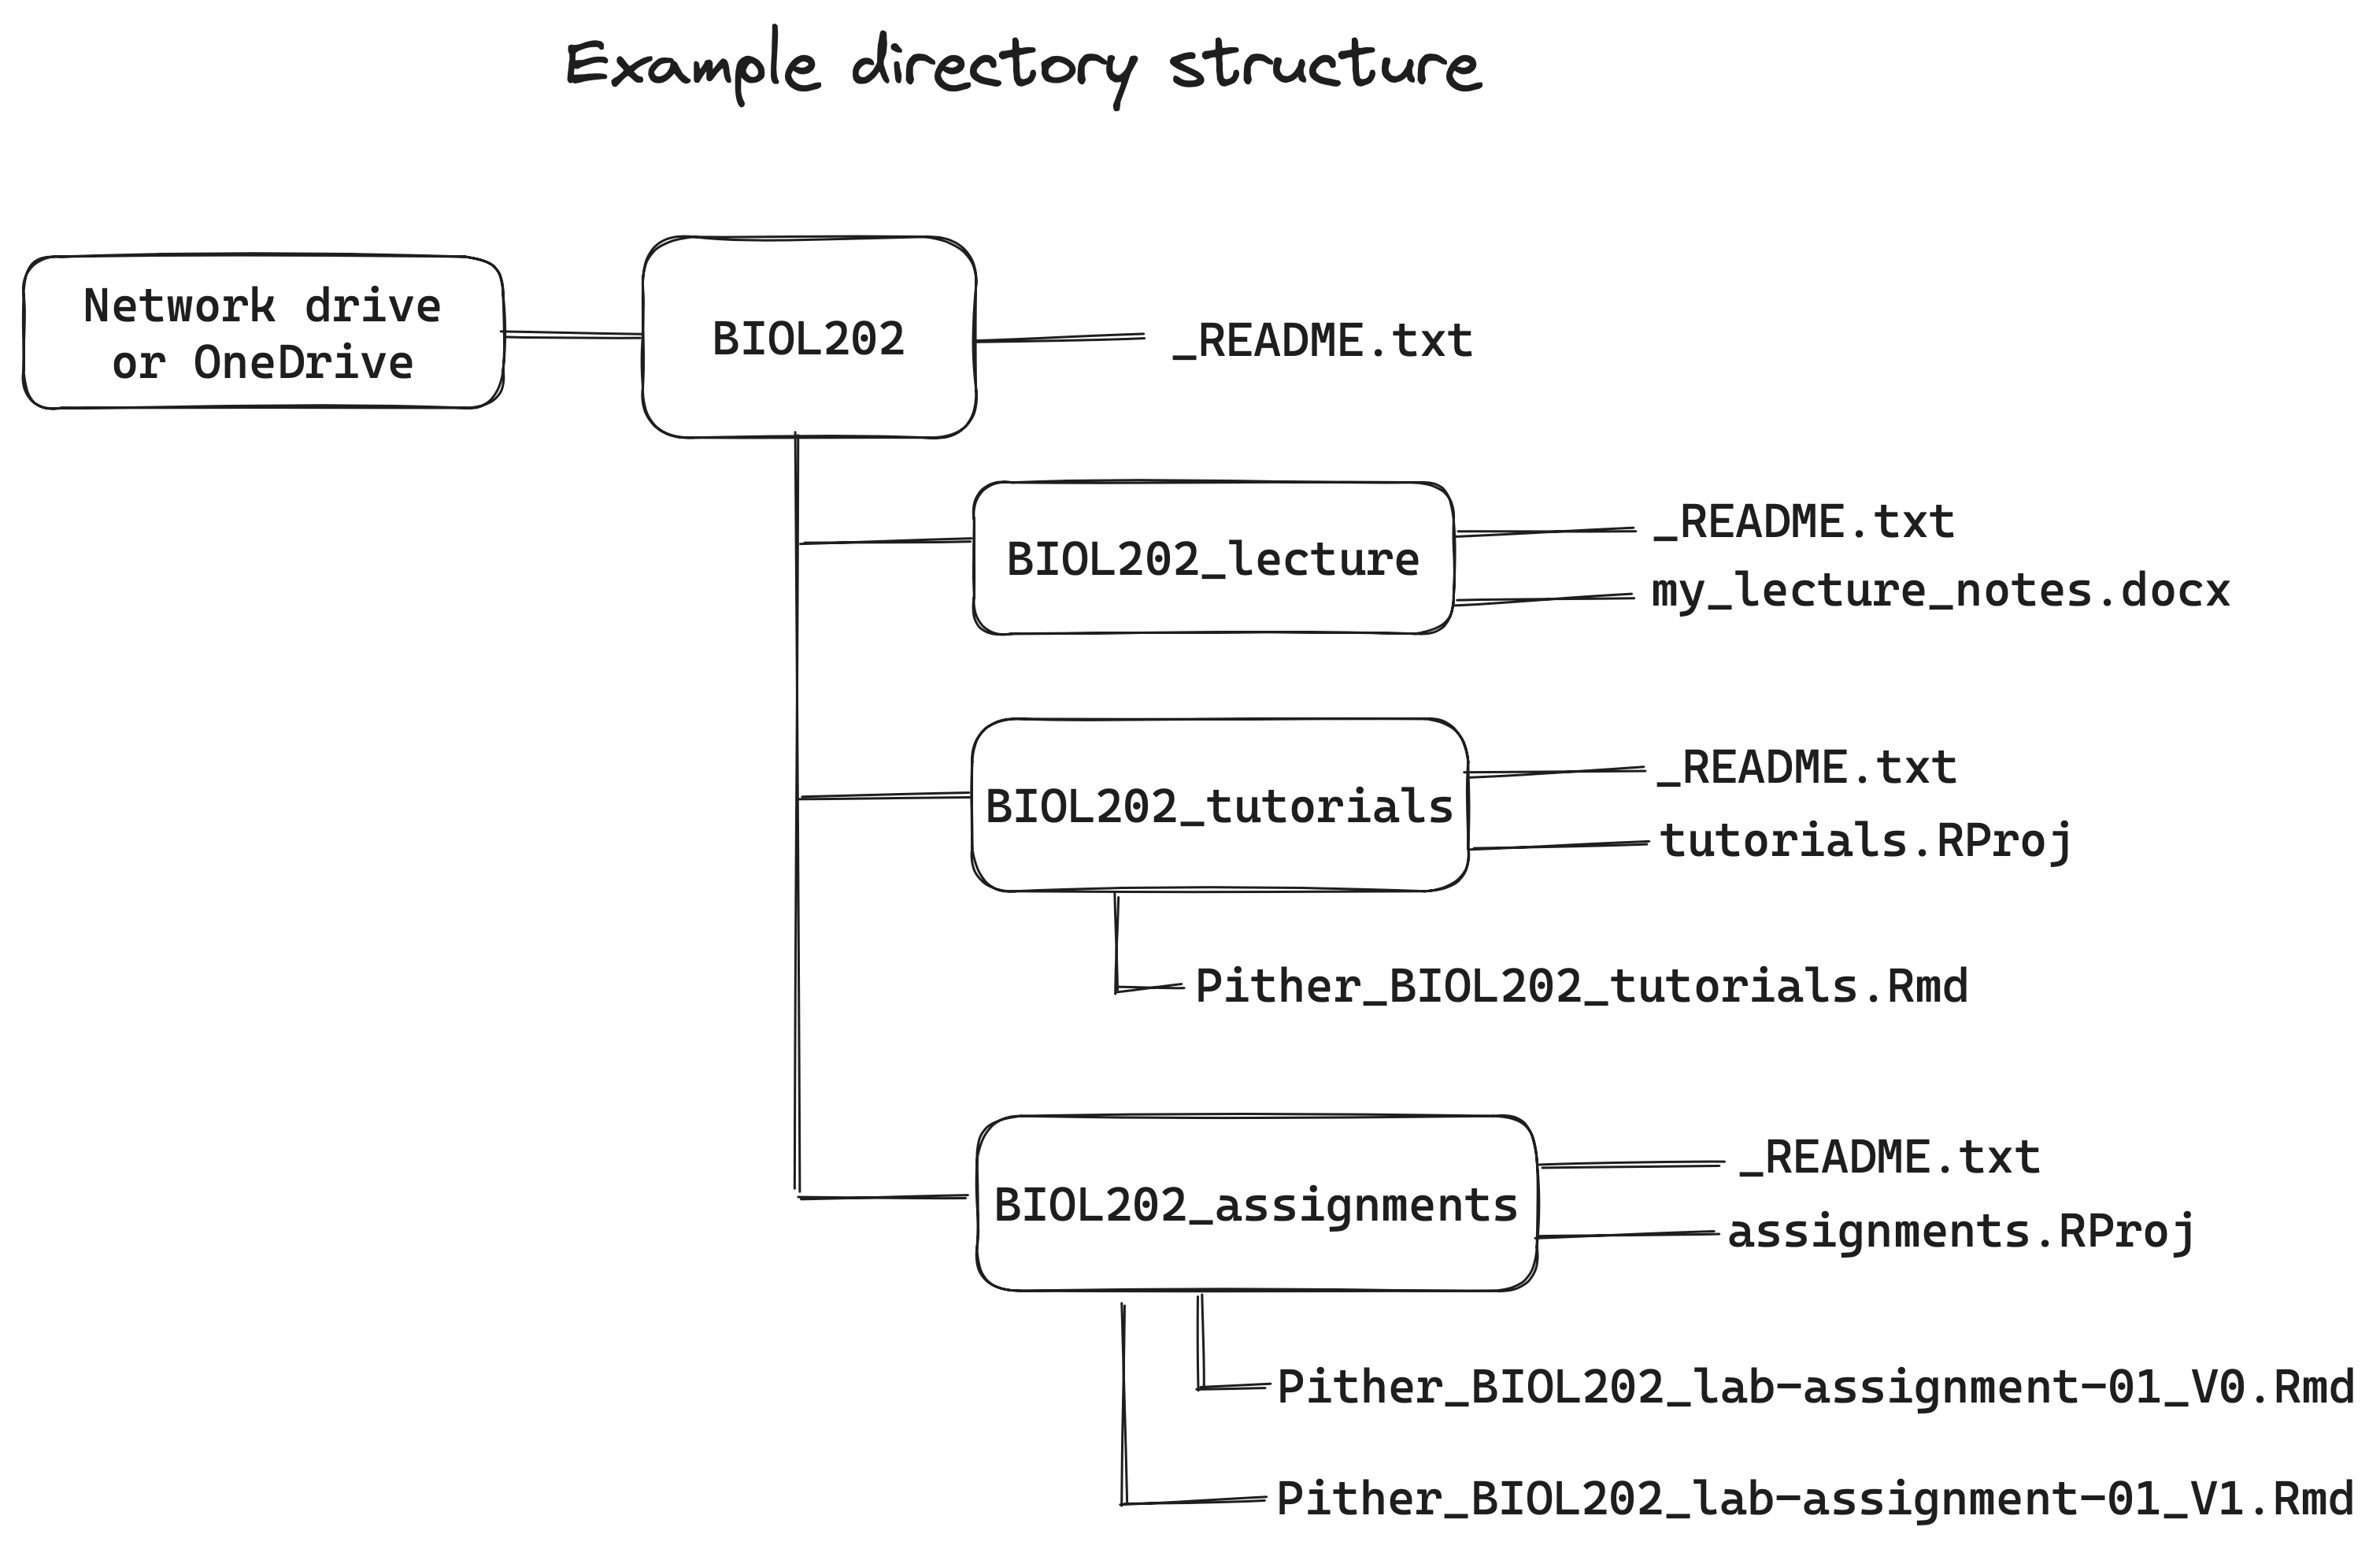
\includegraphics[width=41.99in]{./more/BIOL202_directory_structure} \caption{Example directory structure}\label{fig:unnamed-chunk-9}
\end{figure}

The BIOL202 directory, and all its contents, will now sync regularly to your online OneDrive account, so that you can access your up-to-date files from any device upon which OneDrive is installed.

It is possible to work on files stored on your local computer when you're offline; they just won't sync to the cloud until you've gotten back online.

\section{Lecture workflow}\label{lecture_workflow}

The directory for your lecture work is now ready to house any lecture-related work that you do. For instance, if you wish to type up study notes in a Word document, you could call that file ``Pither\_BIOL202\_lecture-notes.docx''. Each time you add/edit/update it, OneDrive will keep old versions for you!

\section{Tutorial workflow}\label{tutorial_workflow}

How you manage your tutorial workflow comes down to personal preference. The instructions provided below create an RStudio project in the ``BIOL202\_tutorials'' directory (see below), and then create a single R Markdown document, formatted to have sections (headers) for each tutorial you work on. This approach makes it easier to find all of your work in the R Markdown file, so long as it is formatted logically.\\
I have created an R Markdown file that you can download and use for this purpose, and we'll download that a bit later.

First, we need to set up an RStudio project.

\section{Create an RStudio Project}\label{create_project}

It is best to organize all your R work using RStudio ``projects''. For your tutorial work, for example, you will create a new project that will be housed in your ``BIOL202\_tutorials'' directory

To do this, open RStudio then select File \textgreater{} New Project. Then select the option to use an existing directory, and locate and select your tutorial directory. Provide a name for your project file, such as ``BIOL202\_tutorial'', then select OK. If it asks to open a new RStudio session, you can say yes.

RStudio has now created an RStudio project file that has an ``Rproj'' extension at the end of the name. This ``Rproj'' file is the file that you will open (double-click with the mouse) each time you wish to work on your tutorial material. You should see the ``Rproj'' file in the bottom right files panel of RStudio.

\section{Create subdirectories}\label{create_subdirs}

Your tutorial work may involve creating and saving outputs like figures or files, in which case you should have sub-directories for these purposes in your root directory. See the example provided in the \href{https://ubco-biology.github.io/Procedures-and-Guidelines/example-biol-116.html\#screenshot}{Procedures and Guidelines document}.

Let's illustrate the procedure by creating a subdirectory called ``figures'', and this time we'll use R to create the directory.

The following code will create a directory called ``figures'' in your working directory

\begin{verbatim}
dir.create("figures")
\end{verbatim}

You should see the new folder appear in the files panel on the bottom right of RStudio.

Whenever you wish to generate figures in R, then export them as image files, for example, you can save them to this folder. We'll learn about this later.

Reading and writing files from / to directories requires that we can tell R exactly where to find those directories. That's where the handy package called \texttt{here} comes in.

\subsection{\texorpdfstring{The \texttt{here} package}{The here package}}\label{here_package}

Now we'll install and load an R package called \texttt{here} that will help with file and directory management and navigation.

\begin{verbatim}
install.packages("here")
\end{verbatim}

This is a helpful \href{http://jenrichmond.rbind.io/post/how-to-use-the-here-package/}{blog post} about the utility of the \texttt{here} package.

Then we load the package:

\begin{Shaded}
\begin{Highlighting}[]
\FunctionTok{library}\NormalTok{(here)}
\end{Highlighting}
\end{Shaded}

When you load the package, the \texttt{here} function takes stock of where your RStudio project file is located, and establishes that directory as the ``working directory''. It should return a file path for you. In future tutorials we'll make use of the \texttt{here} package when saving files.

\section{Edit an R markdown file}\label{edit_markdown}

In a previous \hyperref[intro_markdown]{tutorial} you learned how to create an R Markdown file, but generally you won't need to do this in this course, because you'll be provided starter documents to work with.

I have created an R Markdown file that you can download and use for starting your tutorial work.

To do this, type the following code into your command console in RStudio (the bottom left panel):

\begin{Shaded}
\begin{Highlighting}[]
\FunctionTok{download.file}\NormalTok{(}\StringTok{"https://raw.githubusercontent.com/ubco{-}biology/BIOL202/main/more/Example\_tutorial\_markdown.Rmd"}\NormalTok{, }\StringTok{"BIOL202\_tutorial\_markdown.Rmd"}\NormalTok{)}
\end{Highlighting}
\end{Shaded}

This \texttt{download.file} command takes a URL address for a file stored online, and then tells R where to save it, and what name to use.

Here we will save the RMD file in your ``working directory'', which is the ``BIOL202\_tutorials'' directory. It should show up in the ``files'' pane in the bottom right RStudio panel. Click on the ``BIOL202\_tutorial\_markdown.Rmd file to open it.

This is the R Markdown file that you'll edit/add to throughout the term. It has some starting instructions / example text already, and you're welcome to delete / change that.

\begin{itemize}
\tightlist
\item
  Change the ``author'' information at the top of the document (in the header) to your name.
\item
  Save your file by clicking the save icon in the top left, and be sure to give it an appropriate name as per previous file-naming instructions
\end{itemize}

For the basics on formatting in R Markdown, consult the R Markdown \href{https://www.rstudio.com/wp-content/uploads/2015/03/rmarkdown-reference.pdf}{reference guide}

\section{Components of an R Markdown file}\label{md_components}

At this point, you should familiarize yourself with the components of a markdown file.

\begin{center}\rule{0.5\linewidth}{0.5pt}\end{center}

\begin{enumerate}
\def\labelenumi{\arabic{enumi}.}
\tightlist
\item
  R basics
\end{enumerate}

Read through section 4.2 of this online \href{https://rbasics.netlify.app/4-rmarkdown.html\#the-components-of-an-r-markdown-file}{tutorial} and watch the videos there too

\begin{center}\rule{0.5\linewidth}{0.5pt}\end{center}

\section{Interacting with Tutorial material}\label{interact_tutorial}

Students have typically worked through tutorials by reading the material, typing helpful notes in their markdown document, and typing the provided R code into ``chunks'' within their R Markdown document, then running those chunks. (\textbf{NOTE}: it's better for you to practice typing the code, rather than copying and pasting!)

You can insert as many chunks as you'd like. Chunk insertion is achieved by selecting the green ``+'' icon at top of the editor panel, and selecting ``R''. Or go to the ``Code'' menu drop down and ``Insert Chunk''.

The key advice: keep your work organized by using headings. There's an option to view your headings all in one navigation pane by clicking on the navigation pane icon at the top right of your editor panel.

\section{Lab assignments workflow}\label{assign_workflow}

You can repeat the same steps from earlier for creating a new \hyperref[create_project]{RStudio project} for your lab work. But this time when you create the project, specify your lab assignment directory ``BIOL202\_assignments'' as the location.

You can optionally create subdirectories also, perhaps one for each of the lab assignments.

The key difference in the assignments workflow is that for each assignment you'll start with a new R Markdown (Rmd) file, which you'll download from Canvas under the ``assignments'' link. The document will include the questions you are to answer, and you simply edit / add to the document as you answer them.

Instructions for this will come in a later tutorial.

Next tutorial: Practicing completing a very short lab assignment using R Markdown.

\chapter{Preparing and formatting assignments}\label{prepare_assignments}

This material provides instructions on how to prepare and format R Markdown documents for assignments.

\section{Open your assignment RStudio project}\label{open_assign_project1}

In a previous \hyperref[assign_workflow]{tutorial} it was suggested you set up a working root directory called ``BIOL202\_assignments'' to host all your assignment work. You may have also created sub-directories, one for each of the three assignments. Regardless, in your root ``BIOL202\_assignments'' directory locate the RStudio project file (it has a ``Rproj'' extension in the filename), and open it by double-clicking it.

\section{Download the assignment Rmd file}\label{download_assign_rmd}

The assignment file will be available to you for download from Canvas under the ``Assignments'' section. The file is actually an R Markdown file, and therefore has an ``Rmd'' extension. It is simply a text document (meaning it contains only text), but the syntax used therein is ``markdown'' syntax, and the file extension (Rmd) specifies it as an R Markdown file. You might recall reading about Markdown in the \href{https://ubco-biology.github.io/Procedures-and-Guidelines/markdown-1.html}{Biology Procedures and Guidelines document}.

Make sure you save the Rmd file into your root ``BIOL202\_assignments'' directory, or alternatively into the appropriate sub-directory.

A small assignment has been set up on Canvas, with the aim of you getting use to the assignment procedure. It is located under ``Lab\_materials'' module. Download the file, and make sure it's saved into your root directory (where your RStudio project is).

\section{Open the assignment Rmd file}\label{open_rmd_file}

In RStudio, look in the ``files'' pane (bottom right) and locate your downloaded assignment Rmd file. Then click it to open.

This Markdown document includes the assignment questions, and serves as a starter document for your assignment.

Once you have opened the document, you'll see the following text at the top:

\begin{figure}
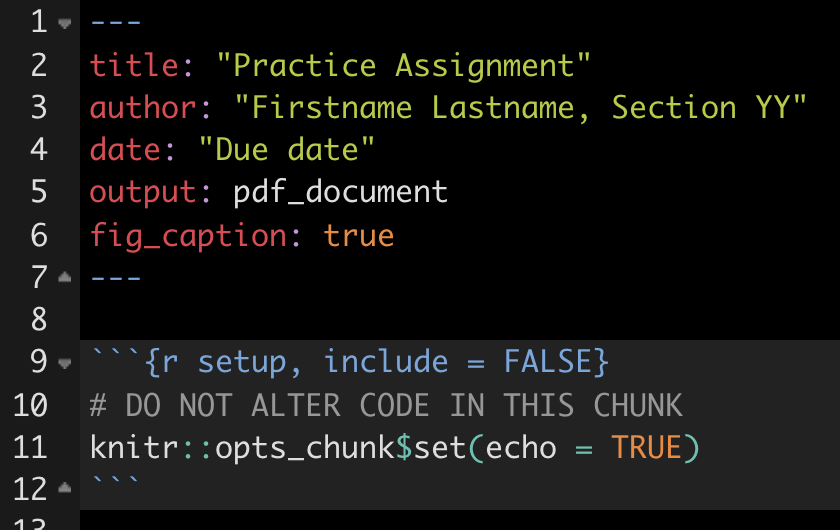
\includegraphics[width=11.67in]{./more/assign_header} \caption{Assignment markdown file header}\label{fig:unnamed-chunk-11}
\end{figure}

Complete the following steps:

\begin{itemize}
\tightlist
\item
  keeping the quotation marks, replace the ``Practice assignment'' text with the current assignment name\\
\item
  keeping the quotation marks, replace the ``Firstname Lastname, Section YY'' with your own Firstname Lastname and section number (e.g.~'' Jason Pither, Section 04'')
\item
  keeping the quotation marks, replace the ``Due date'' with the due date of the current assignment, e.g.~``September 21, 2022''
\end{itemize}

Don't alter anything else at the top of the document, including the R Chunk that you see below the header.

\begin{itemize}
\tightlist
\item
  save the Rmd file using a new name (so select file \textgreater{} ``save as''), according to appropriate \href{https://ubco-biology.github.io/Procedures-and-Guidelines/file-and-data-management.html}{file naming conventions}, such as ``Pither\_BIOL202\_lab-assignment-01\_V0.Rmd''. Recall that if you're saving this on OneDrive, or in your local directory that is synced to OneDrive, then your file will be \hyperref[onedrive]{version controlled}, so you don't need to include a version number (``\_V0'') in the filename.
\end{itemize}

You're now ready to start working on your assignment, and doing \href{https://ubco-biology.github.io/Procedures-and-Guidelines/glossary.html}{literate programming} using R Markdown.

In RStudio, under the ``Help'' menu, you'll find ``Cheat Sheets'' \textgreater{} R Markdown Cheat Sheet and R Markdown Reference Guide. Have a look at those!

\section{What to include in your answers}\label{what_include_answer}

The general approach is to enter your text answers and associated R chunks with code underneath each question.

\textbf{TIP}: It is almost always the case that you'll need to load the \texttt{tidyverse} package, so it's advisable to include an R chunk right at the beginning of your document that does this.

\textbf{TIP}: To insert a new code chunk, you can either: Use the shortcut: Mac = \texttt{Command+Option+I}; Windows = \texttt{Ctrl+Alt+I}. Click on the \textbf{Insert a new code chunk} icon. You can also specify the coding language of the chunk using the drop-down menu.

\subsection{Code chunk headers}\label{chunk_headers}

Here's an example code chunk in which the \texttt{tidyverse} package is being loaded. You'll notice some extra text in the header of the chunk.

\begin{figure}
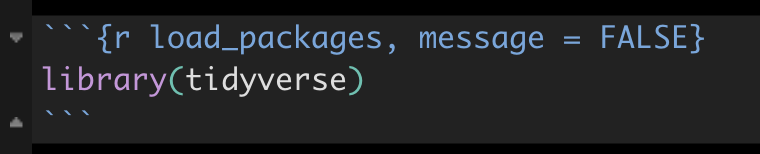
\includegraphics[width=10.56in]{./more/install_package_header2} \caption{Code chunk header with message suppression}\label{fig:unnamed-chunk-12}
\end{figure}

The ``load\_packages'' text is simply giving a name or ``tag'' to this R chunk. It is good practice to provide a \emph{unique} name to each R chunk.

After the comma is \texttt{message\ =\ FALSE}. This tells R markdown to NOT display any messages associated with the R commands in this chunk when knitting the R Markdown document. For example, when loading some libraries R will provide a long list of messages in the process. When you ``knit'' the R Markdown document, R will run each R chunk in your document. By including the \texttt{message\ =\ FALSE} heading argument, you can avoid including this extra output in your knitted document.

The \texttt{message\ =\ FALSE} header argument is NOT something to include in all chunks by default. It should only be included if the code within the associated code chunk outputs a lot of unnecessary information that would otherwise clutter your knitted PDF document.

\begin{center}\rule{0.5\linewidth}{0.5pt}\end{center}

There will be routine steps to take for each question.

\subsection{Import data}\label{first_csv_import}

Each assignment question will indicate which dataset(s) you'll need to answer the question, and where to locate / download these. In many instances multiple questions will use the same dataset, in which case you don't need to load data for each question; just load it once.

Here's an example of code for importing data. It uses the \texttt{read\_csv} function from the \texttt{readr} package, which is bundled with the \texttt{tidyverse} package:

\begin{verbatim}
example_data <- read_csv("https://raw.githubusercontent.com/ubco-biology/BIOL202/main/data/example_data.csv")
\end{verbatim}

The \texttt{read\_csv} function will take as an argument a URL address for a data file. Here we've provided a URL for the location of a CSV file (comma-separated values file), which is typically what we'll use.

\subsection{Load packages}\label{first_load_package}

Once you've loaded the data, you'll now need to figure out how to answer the question by looking through the tutorials for the answer. And typically, to answer the question you'll need to make sure you've loaded some packages.

If you've forgotten what ``packages'' are, refresh your memory at this \hyperref[packages]{tutorial}.

For example, it's likely you've already loaded the \texttt{tidyverse} package (as advised above), but if a tutorial indicates you need another package, say the \texttt{janitor} package, then insert a code chunk with the following:

\begin{verbatim}
library(janitor)
\end{verbatim}

When working on your own computer, you only need to install a package once (unless you want to update an already installed package to the latest version, which is a rare event). If you're working on a school computer (in a computer lab), you may need to install packages each time you log on to a computer, because the school computers delete local files daily. If you're unsure what packages are already installed, consult the ``packages'' tab in the lower-right RStudio pane when you start up RStudio; installed packages are listed there.

\subsection{Answer the questions}\label{answer-the-questions}

After you've imported the required data and loaded required packages, it's time to answer the questions!

You simply insert any required text and R code (in R Chunks) after each question. The tutorials will provide the information required to answer the questions.

\textbf{TIP}: The way to test out your code once it's inserted in the R chunk is to press the green play button at the top right of the code chunk. This will run what's in the chunk. You'll be provided error statements if something goes wrong. If it works, it will provide you the output (and hopefully the answer!), and this is what you use to inform your written (typed) answer.

Here's what you need to include in your answers:

\begin{itemize}
\item
  Answer each question clearly and in full sentences. Make sure you answer specifically the question asked.
\item
  Verify that the code you used to answer the question is included in an R chunk and appears in the knitted document (this should happen automatically)
\item
  Verify that the output from each R chunk is included in your knitted document (this should happen automatically)
\item
  For any figures (graphs) that you produce, you must include a figure caption. See the next \hyperref[rmd_graphing]{section} for instructions.
\item
  If you use a graph to answer a question, refer to that graph in your answer
\end{itemize}

\textbf{REMINDER}: As you work on your document, save frequently, and also knit your document frequently.

\textbf{TIP}: You will often need/want to preview the document you are working on to ensure that everything is being formatted as you expected in the knitting process. The default setting is for the preview to open in a new pop-up window outside of RStudio, although you may find it useful to have it open in the Viewer panel within RStudio itself (particularly if you're only working with one screen!). To change the preview location, click the \textbf{Settings} icon in the toolbar and select the option to ``Preview in Viewer Pane''.

\section{Setting up R Markdown for graphing}\label{rmd_graphing}

There are some special code chunk header arguments that need to be set in your Markdown document in order to:

\begin{itemize}
\tightlist
\item
  include proper \textbf{Figure captions} with your figures (a necessity!)
\item
  set the dimensions of your figures
\end{itemize}

In each code chunk that includes code to construct a graph, your chunk header options should look like this in the top of the chunk, and there should be one blank line underneath before the main code starts. The following chunk produced the figure below. And recall that in the example below, the ``bill\_fig'' text is simply the name I've given to this code chunk.

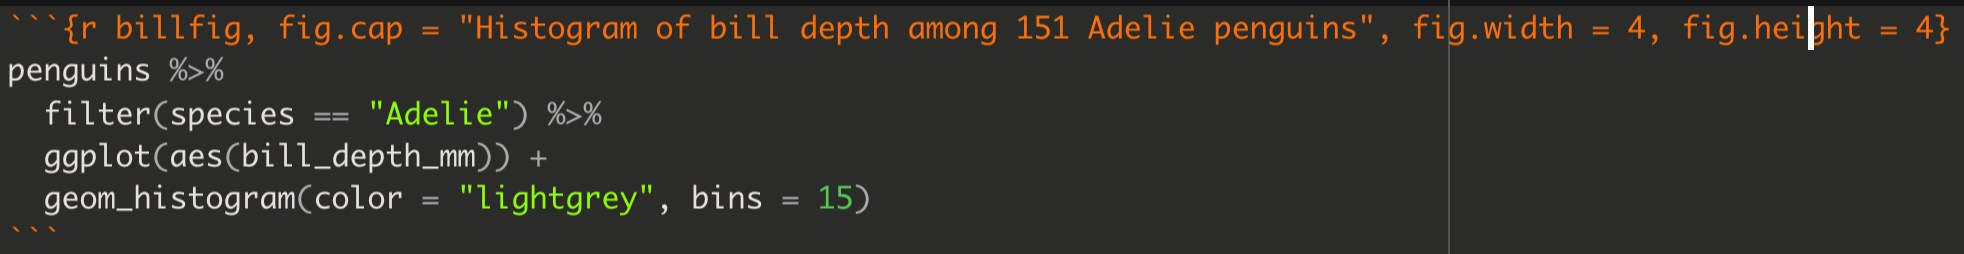
\includegraphics[width=33.92in]{./more/figure_chunk_header}

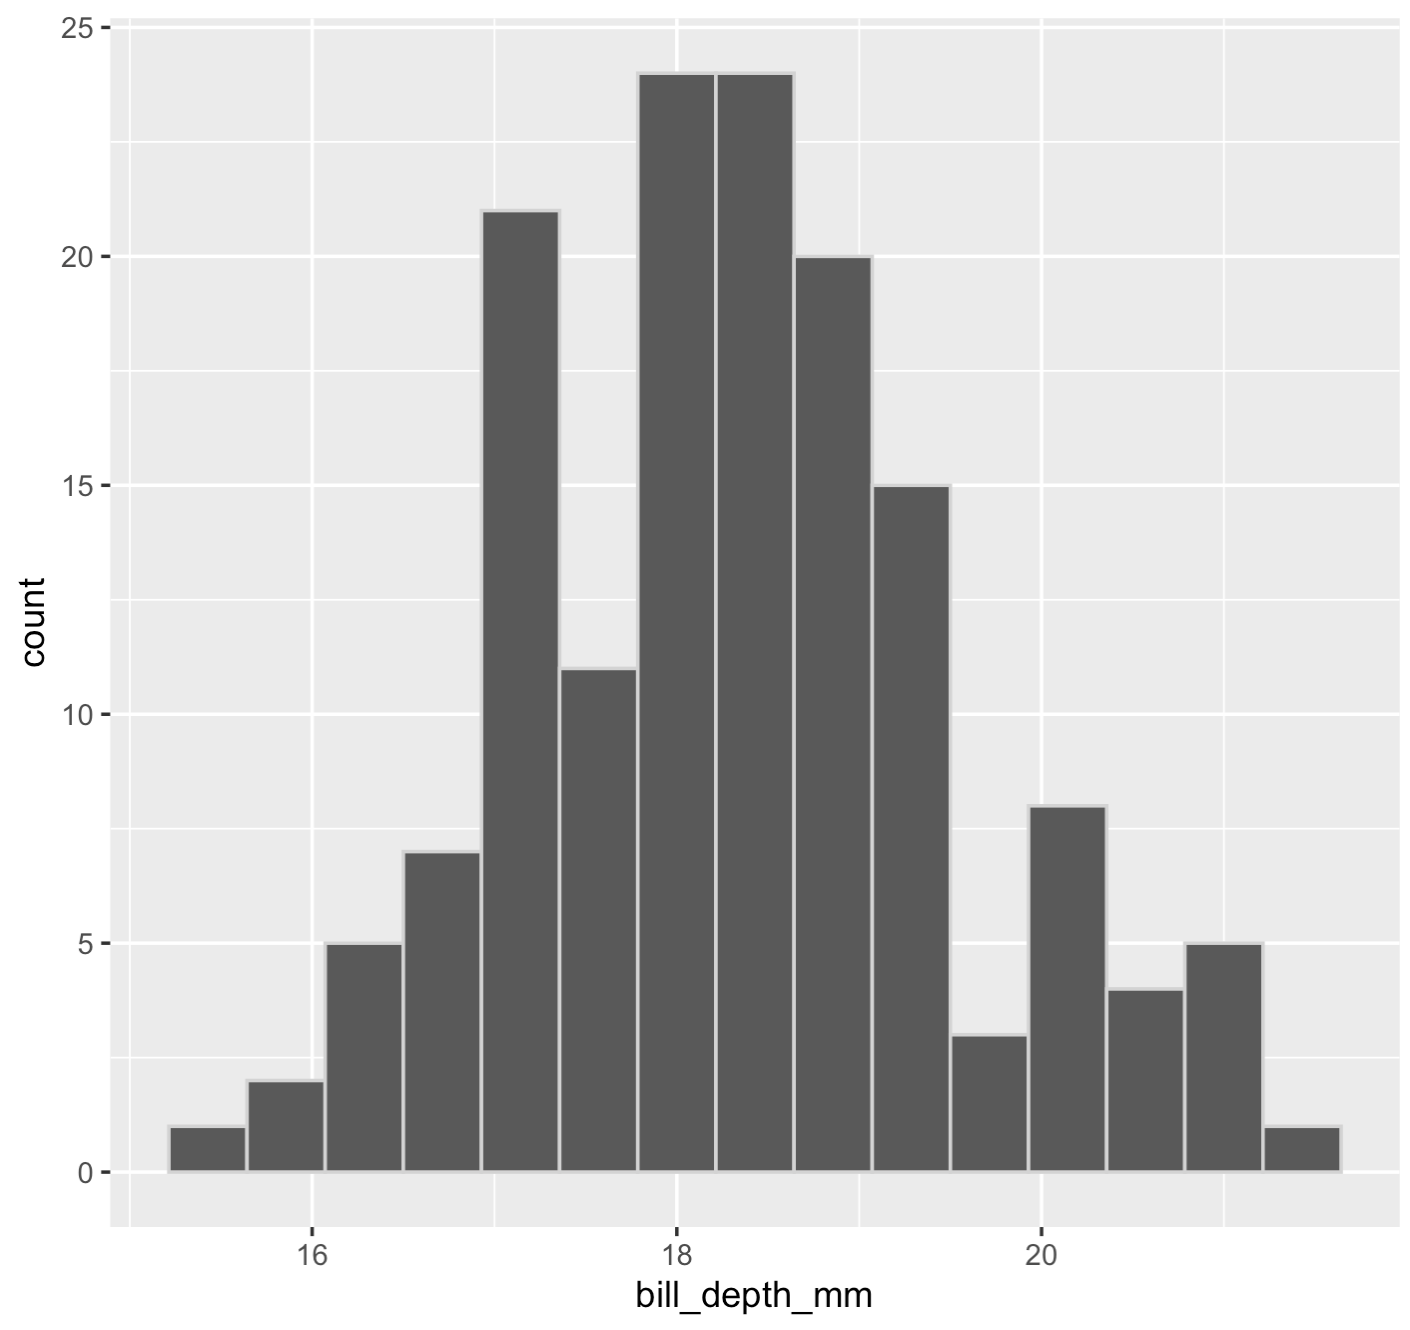
\includegraphics[width=19.58in]{./more/example_histogram_practice}

\textbf{Figure 1:} Histogram of bill depth among 151 Adelie penguins

The key parts are the ``fig.cap ='' argument, to which you provide the text you want to use as the figure caption. Then there's the ``fig.width ='' and ``fig.height ='' arguments, which indicate the size of the figure when knitted. This will likely require some trial-and-error to get a good size, but start with the values in this example (4 for each).

\textbf{Automated figure numbering}

When you knit the document to PDF, you'll see the ``Figure X:'' (with a number in place of the ``X'') text was appended at the beginning of the caption phrase that was included in the chunk header, ``Histogram of bill depth among 151 Adelie penguins''.

This feature - automatic figure numbering - was set within the header of the assignment markdown document:

\begin{figure}
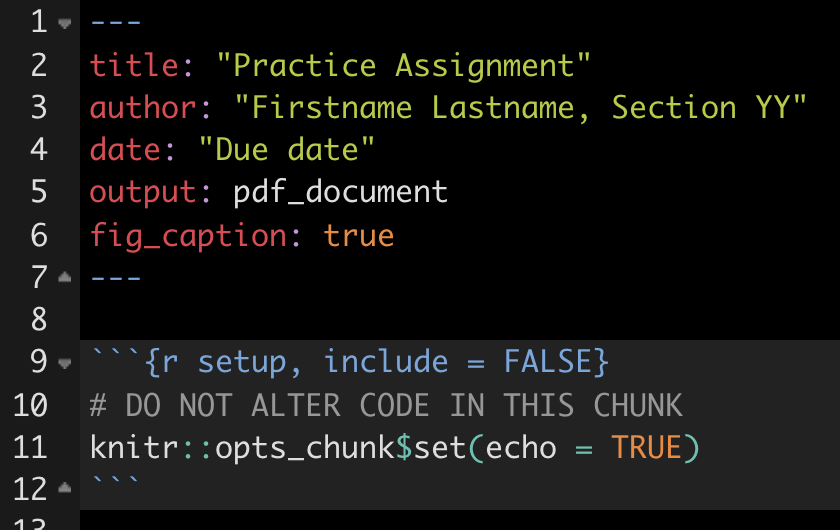
\includegraphics[width=11.67in]{./more/assign_header} \caption{Assignment markdown file header with figure caption option}\label{fig:unnamed-chunk-15}
\end{figure}

The line ``fig\_caption = true'' tells R Markdown and the knitting process to automatically include this part of a figure caption, ``Figure X'', underneath each figure you produce. Where ``X'' will automatically be replaced with the appropriate number. For example, it will use ``Figure 1:'' for your first figure, ``Figure 2'' for your second, and so on.

The figure captions will only appear correctly once you knit to PDF; captions do not appear in the preview provided within the editor pane.

\section{Example question / answer}\label{example_answer}

Below is an example of how to answer a question. You haven't yet learned some of the functions we use here, but follow along for now - it's just an example!

There are almost \emph{always} multiple coding approaches to get the right answer, some better than others. As long as your code and answer are accurate and make sense, you'll get the marks!

\textbf{Question 1.} What are the minimum and maximum heights (variable name is ``height\_cm'') of students in the ``students'' dataset, which is available at this URL:

\begin{verbatim}
https://raw.githubusercontent.com/ubco-biology/BIOL202/main/data/students2.csv
\end{verbatim}

As we learned in the {[}fictitious{]} ``importing and exploring data'' tutorial, I can use the \texttt{read\_csv} function from the \texttt{readr} package (loaded with \texttt{tidyverse}) to download and import the dataset. It creates a ``tibble'' object, which here I name ``students'':

\begin{Shaded}
\begin{Highlighting}[]
\NormalTok{students }\OtherTok{\textless{}{-}} \FunctionTok{read\_csv}\NormalTok{(}\StringTok{"https://raw.githubusercontent.com/ubco{-}biology/BIOL202/main/data/students.csv"}\NormalTok{)}
\end{Highlighting}
\end{Shaded}

I also learned that it's a good idea to get an overview of the dataset as a first step after importing data. To do this, use the \texttt{skim\_without\_charts} function from the \texttt{skimr} package. I need to load that package first:

\begin{Shaded}
\begin{Highlighting}[]
\FunctionTok{library}\NormalTok{(skimr)}
\end{Highlighting}
\end{Shaded}

Now skim:

\begin{Shaded}
\begin{Highlighting}[]
\FunctionTok{skim\_without\_charts}\NormalTok{(students)}
\end{Highlighting}
\end{Shaded}

(\#tab:skim\_data)Data summary

Name

students

Number of rows

154

Number of columns

6

\_\_\_\_\_\_\_\_\_\_\_\_\_\_\_\_\_\_\_\_\_\_\_

Column type frequency:

character

3

numeric

3

\_\_\_\_\_\_\_\_\_\_\_\_\_\_\_\_\_\_\_\_\_\_\_\_

Group variables

None

\textbf{Variable type: character}

skim\_variable

n\_missing

complete\_rate

min

max

empty

n\_unique

whitespace

Dominant\_hand

0

1

1

1

0

2

0

Dominant\_foot

0

1

1

1

0

2

0

Dominant\_eye

0

1

1

1

0

2

0

\textbf{Variable type: numeric}

skim\_variable

n\_missing

complete\_rate

mean

sd

p0

p25

p50

p75

p100

height\_cm

0

1

171.97

10.03

150

165.00

171.48

180.0

210.8

head\_circum\_cm

0

1

56.04

6.41

21

55.52

57.00

58.5

63.0

Number\_of\_siblings

0

1

1.71

1.05

0

1.00

2.00

2.0

6.0

This shows we have four character and three numeric variables, with 154 rows (observations) and 7 columns (variables) total.

We can use the \texttt{summary} function to get some basic descriptive statistics, including the minimum and maximum of numeric variables. The \texttt{summary} function is part of the base R package, so no additional packages need to be loaded.

We also use the \texttt{select} function from the \texttt{dplyr} package (which is loaded with \texttt{tidyverse}) to select which variable in the \texttt{students} tibble we wish to summarize.

The use of the ``\%\textgreater\%'' syntax is described in a later tutorial.

\begin{Shaded}
\begin{Highlighting}[]
\NormalTok{summary.height }\OtherTok{\textless{}{-}}\NormalTok{ students }\SpecialCharTok{\%\textgreater{}\%} 
  \FunctionTok{select}\NormalTok{(height\_cm) }\SpecialCharTok{\%\textgreater{}\%}
\NormalTok{  summary}
\NormalTok{summary.height}
\end{Highlighting}
\end{Shaded}

\begin{verbatim}
##    height_cm    
##  Min.   :150.0  
##  1st Qu.:165.0  
##  Median :171.5  
##  Mean   :172.0  
##  3rd Qu.:180.0  
##  Max.   :210.8
\end{verbatim}

As shown in the output above, the minimum height was 150.0 cm and the maximum student height was 210.8 cm.

\textbf{TIP}: You'll note that functions and package names above are highlighted in grey. When writing in markdown, it's good practice to encompass function names and package names in single backticks, i.e.\texttt{\textasciigrave{}tidyverse\textasciigrave{}}. Backticks are typically located with the tilden (``\textasciitilde{}'') key on your keyboard.

\section{Knitting your assignment to PDF}\label{knit_assign}

All assignments are to be submitted to Canvas as \textbf{PDF documents}.

As you learned in a previous \hyperref[veryify_knit]{tutorial}, simply click on the ``knit'' button and select PDF. Your PDF file will adopt the same name as your markdown file, but it will have a ``pdf'' extension rather than an ``Rmd'' extension.

Once you have knitted your assignment to PDF, open up the PDF document, and verify that it looks correct, and be sure to check all your spelling, and that figures / tables are appropriately formatted etc\ldots{}

If you need to fix something, close your PDF file, go back to your R Markdown document and do the edits there. Save, then knit again!

\section{Submit your assignment}\label{submit_rmd}

Once you're happy with the PDF you created, it's time to submit \textbf{both your markdown file (.Rmd file) and your PDF document} to the appropriate place in Canvas. Submitting both files enables markers to check where things went wrong if there are any knitting errors.

It's a good idea also to verify afterwards that your PDF document did indeed upload correctly.

\chapter{Preparing and importing Tidy Data}\label{data_import}

\textbf{Tutorial learning objectives}

In this tutorial you will:

\begin{itemize}
\tightlist
\item
  Review how to format your data

  \begin{itemize}
  \tightlist
  \item
    \href{https://ubco-biology.github.io/Procedures-and-Guidelines/tidy-data.html}{Tidy data}
  \item
    Do's and Don'ts of naming variables and data entry
  \item
    Wide versus Long format
  \end{itemize}
\item
  Learn how to save a file in CSV (comma-separated values) format\\
\item
  Learn how to import a CSV file from a website into a \texttt{tibble} in R\\
\item
  Learn how to import a CSV file from a local directory into a \texttt{tibble} in R\\
\item
  Learn how to get an overview of the data and variables in your \texttt{tibble}
\end{itemize}

Importing data should be a straightforward task, but this is not always the case; sometimes data files are not formatted properly, so you need to be careful to check what you import.

Here, you'll learn (or review) how to format your own data files according to best practices, so that you or others will have no problems importing them.

It is assumed that if you are collecting data during a project, you'll likely enter them on your computer using a spreadsheet software program like Excel.

\textbf{PAUSE}: Before starting any data collection and data-entry, ask yourself: how should I organize the spreadsheet for data-entry?

The short answer: according to \textbf{TIDY} formatting principles\ldots{}

\section{Tidy data}\label{tidy_data}

Review the \href{https://ubco-biology.github.io/Procedures-and-Guidelines/tidy-data.html}{Biology Procedures and Guidelines document} chapter on \textbf{Tidy data}.

There you'll learn how to arrange and format your data within a spreadsheet. The ``Tidy'' example provided would look like this in Excel:

\begin{figure}
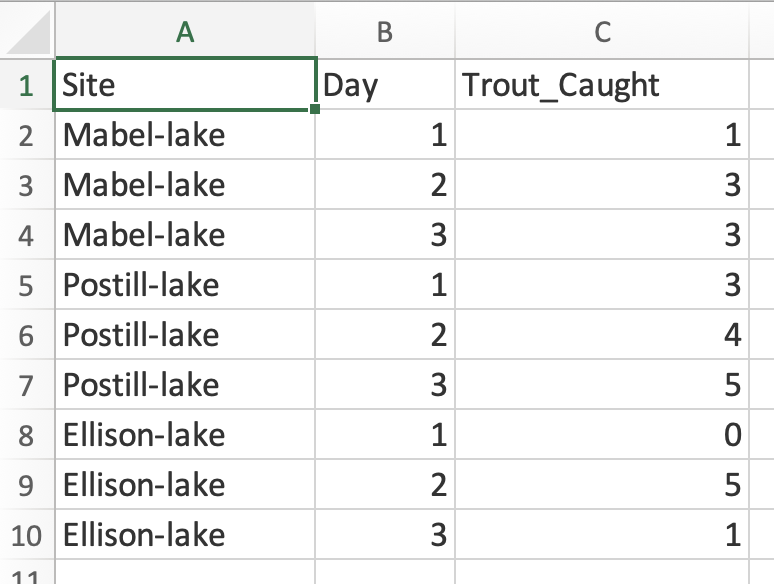
\includegraphics[width=10.75in]{./more/excel_tidy} \caption{Tidy data in Excel}\label{fig:unnamed-chunk-16}
\end{figure}

If you'd like a longer, more in-depth read about ``tidy data'', see Hadley Wickham's ``R for Datascience'' online book, linked \href{http://r4ds.had.co.nz/tidy-data.html}{here}.
And this \href{https://towardsdatascience.com/tidy-data-with-r-f3d078853fc6}{article} describes why making your data ``tidy'' saves a lot of time and effort in the long run. Oh, and it uses Covid-19 data to demonstrate!

If you wish to import and analyze data that have not been formatted according to \textbf{tidy} principles, then the most transparent and computationally reproducible way to reformat the data is to do so by coding \emph{within R}, rather than using software like Excel. The process of reformatting / rearranging data is called \textbf{data wrangling}, and is mostly beyond the scope of this course.

If you're curious about data wrangling, the \texttt{dplyr} package, which is loaded with the \texttt{tidyverse} package, provides all the tools for data wrangling. Its associated cheatsheet is available \href{https://www.google.com/url?sa=t&rct=j&q=&esrc=s&source=web&cd=&ved=2ahUKEwiDxcv5zI_6AhWBFzQIHaFDCuMQFnoECBoQAQ&url=https\%3A\%2F\%2Fwww.rstudio.com\%2Fwp-content\%2Fuploads\%2F2015\%2F02\%2Fdata-wrangling-cheatsheet.pdf&usg=AOvVaw3YtyAQzCrVUXwp7frfnZC5}{here}.

\section{Import a CSV file from a website}\label{import_csv_url}

In previous tutorials we've already seen how to import CSV files from the web. As always, the first step is to load the \texttt{tidyverse} library, because it includes many packages and functions that are handy for both data import and data wrangling.

\begin{Shaded}
\begin{Highlighting}[]
\FunctionTok{library}\NormalTok{(tidyverse)}
\end{Highlighting}
\end{Shaded}

One package that is loaded with the \texttt{tidyverse} package is \texttt{readr}, which includes the handy \texttt{read\_csv} function.

You can view the help file for the \texttt{read\_csv} function by typing this into your command console pane (bottom left) in RStudio:

\begin{verbatim}
?read_csv
\end{verbatim}

You'll see that the function has many optional ``arguments'', but in general we can use the default values for these.

If the file you wish to import is located on the web, then we need to provide the ``URL'' (the web address) to the \texttt{read\_csv} function. For example, in \hyperref[example_answer]{a previous tutorial} you imported the ``students.csv'' dataset from the course GitHub website, as follows (and note that the URL address is provided in double quotation marks):

\begin{Shaded}
\begin{Highlighting}[]
\NormalTok{students }\OtherTok{\textless{}{-}} \FunctionTok{read\_csv}\NormalTok{(}\StringTok{"https://raw.githubusercontent.com/ubco{-}biology/BIOL202/main/data/students.csv"}\NormalTok{)}
\end{Highlighting}
\end{Shaded}

\begin{verbatim}
## Rows: 154 Columns: 6
## -- Column specification --------------------------------------------------------
## Delimiter: ","
## chr (3): Dominant_hand, Dominant_foot, Dominant_eye
## dbl (3): height_cm, head_circum_cm, Number_of_siblings
## 
## i Use `spec()` to retrieve the full column specification for this data.
## i Specify the column types or set `show_col_types = FALSE` to quiet this message.
\end{verbatim}

\textbf{PAUSE}: Did you get an error like this?

\textbf{Error in read\_csv(``\url{https://raw.githubusercontent.com/ubco-biology/BIOL202/main/data/students.csv}'') : }
\textbf{could not find function ``read\_csv''}

This happens if you forgot to load the \texttt{tidyverse} library!

The default behaviour of the \texttt{read\_csv} function is to include a printout of the type of variable housed in each column of the dataset. For example, when importing the \texttt{students} dataset, the function gave a printout showing that there are three ``character'' variables (denoted \texttt{chr}) (R calls categorical variables character variables), and three \texttt{dbl} or double precision, floating point format numeric variables.

\begin{enumerate}
\def\labelenumi{\arabic{enumi}.}
\tightlist
\item
  Take a minute to check out this \href{https://www.burns-stat.com/documents/tutorials/impatient-r/more-r-key-objects/more-r-numbers/}{good overview} of how R handles numeric variables.
\end{enumerate}

You can tell R to not provide this information by including the argument \texttt{show\_col\_types\ =\ FALSE} within the \texttt{read\_csv} code. Like so:

\begin{Shaded}
\begin{Highlighting}[]
\NormalTok{students }\OtherTok{\textless{}{-}} \FunctionTok{read\_csv}\NormalTok{(}\StringTok{"https://raw.githubusercontent.com/ubco{-}biology/BIOL202/main/data/students.csv"}\NormalTok{,}
                     \AttributeTok{show\_col\_types =} \ConstantTok{FALSE}\NormalTok{)}
\end{Highlighting}
\end{Shaded}

We have now imported the data and stored it in a local object called ``students''. The object is called a ``tibble'', which you can think of as a special kind of spreadsheet. More information on ``tibbles'' can be found \href{https://r4ds.had.co.nz/tibbles.html}{here}.

Unless otherwise indicated, all CSV data files that we use in this course are stored at the same URL location, specifically: ``\url{https://raw.githubusercontent.com/ubco-biology/BIOL202/main/data/}''. Thus, to import any CSV file you just need to copy that path, then append the appropriate file name to the end of the path. For example, the full path to access a CSV file called \texttt{birds.csv} file would be ``\url{https://raw.githubusercontent.com/ubco-biology/BIOL202/main/data/birds.csv}''.

Often you'll need to import data from a locally stored CSV file, rather than from the web. You'll learn how to do this \hyperref[import_csv_local]{shortly}. First: how does one create a CSV file?

\section{Create a CSV file}\label{create_csv_local}

Before we create or save any data files on our local computer, we should first create a directory (folder) called ``rawdata'' to store them.

Let's create the new directory in our ``BIOL202\_tutorials'' working directory. To do this, use the \texttt{dir.create} function in R, as follows:

\begin{Shaded}
\begin{Highlighting}[]
\FunctionTok{dir.create}\NormalTok{(}\StringTok{"rawdata"}\NormalTok{)}
\end{Highlighting}
\end{Shaded}

Once you run this code, you'll see the new directory appear in the Files pane in the bottom-right of RStudio. It might look something like this:

\begin{figure}
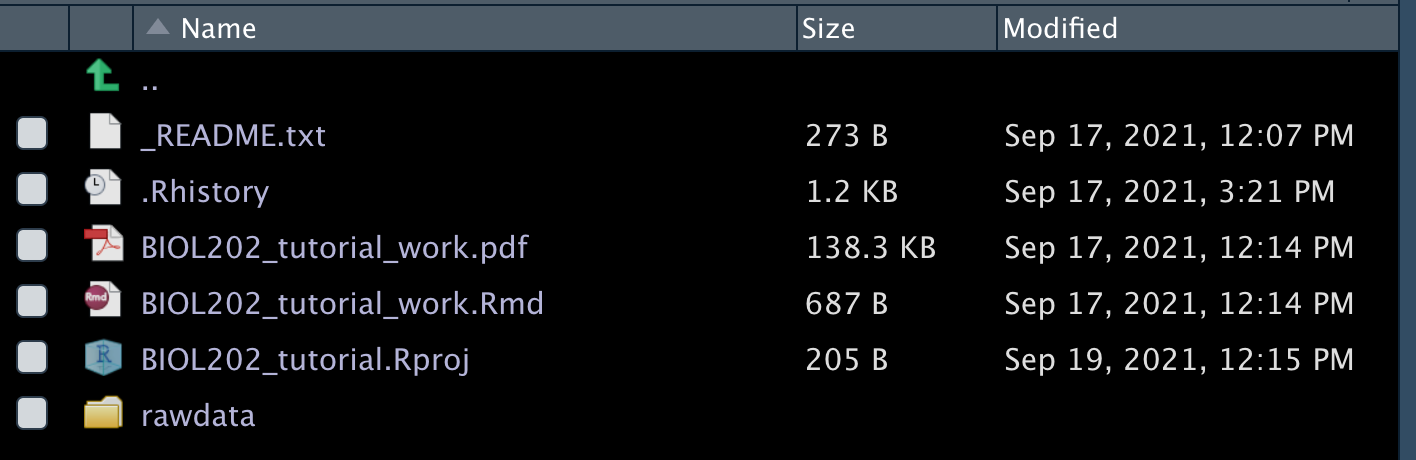
\includegraphics[width=19.67in]{./more/files_pane_rawdata} \caption{View of files with rawdata folder}\label{fig:unnamed-chunk-20}
\end{figure}

The folder is called ``rawdata'' because the data stored there will be the unedited, raw version of the data, and any files therein should \textbf{NOT} be altered. Any changes or edits one makes to the datasets should be saved in new data files that are saved in a different folder called ``output'', which we'll create later.

Let's create a data file to work with.

\textbf{Steps to create and save a CSV file}

\begin{itemize}
\tightlist
\item
  Open up Excel or any other spreadsheet software and enter values in the spreadsheet cells exactly as shown in the Excel example in Figure 10.1 from the \hyperref[tidy_data]{Tidy Data section above}
\item
  You should have one row with the 3 variable names (``Site'', ``Day'', ``Trout\_Caught''), one in each column, then nine rows of data
\item
  Save the file as a CSV file by selecting (MAC) File \textgreater{} Save As \textgreater{} and in the drop down list: CSV UTF-8 (Comma separated), and Windows File \textgreater{} Save as type \textgreater{} CSV UTF-8 (comma separated)
\item
  Name it ``trout.csv'', and save it within the newly created ``rawdata'' folder
\end{itemize}

Now we're ready to try importing the data into a ``tibble''.

\section{Import a local CSV file}\label{import_csv_local}

You can find additional help on importing different types of files at the \href{https://github.com/rstudio/cheatsheets/raw/master/data-import.pdf}{Data Import Cheat Sheet}.

\textbf{Steps to import a local CSV file}

We'll use the ``trout.csv'' file that we created previously.

And we'll make use of the \texttt{here} package that we were introduced to in an \hyperref[here_package]{earlier tutorial}.

Let's load the package:

\begin{Shaded}
\begin{Highlighting}[]
\FunctionTok{library}\NormalTok{(here)}
\end{Highlighting}
\end{Shaded}

\textbf{New tool}: Pipes or ``\%\textgreater\%'' are implemented as part of the \texttt{magrittr} package, which is loaded with the \texttt{tidyverse}. In brief, pipes allow us to string together a series of functions, and we'll use them frequently in tutorials.

Here we'll use a pipe to help import the data file.

Let's see the code first, then explain after:

\begin{Shaded}
\begin{Highlighting}[]
\NormalTok{trout }\OtherTok{\textless{}{-}} \FunctionTok{here}\NormalTok{(}\StringTok{"rawdata"}\NormalTok{, }\StringTok{"trout.csv"}\NormalTok{) }\SpecialCharTok{\%\textgreater{}\%}
  \FunctionTok{read\_csv}\NormalTok{()}
\end{Highlighting}
\end{Shaded}

\begin{itemize}
\tightlist
\item
  First we have the name of the object (a ``tibble'') that we wish to create, ``trout''.
\item
  Then you see the assignment operator ``\textless-'', which tells R to assign whatever we're doing to the right of the operator to the object ``trout''.
\item
  Then we have the \texttt{here} function, which is taking two inputs: the name of the directory we wish to get something from (``rawdata''), and then the name of the file we wish to do something with, here ``trout.csv'').
\item
  Then we have a pipe ``\%\textgreater\%'', which tells R that we're not done coding yet - there's more to come on the next line\ldots{}
\item
  Lastly, we use the \texttt{read\_csv} function, whatever came before the pipe is what is fed to the \texttt{read\_csv} function.
\end{itemize}

Go ahead and run the chunk of code above to create the ``trout'' object.

Next we'll learn how to get an overview of the data stored in a tibble object.

\section{Get an overview of a dataset}\label{data_overview}

When you import data it is always a good idea to immediately get an overview of the data.

Key questions you want to be able to answer are:

\begin{itemize}
\tightlist
\item
  How many variables (columns) are there in the dataset?
\item
  How many observations (rows) are in the dataset?\\
\item
  Are there variables whose data are categorical? If so, which ones?
\item
  Are there variables whose data are numerical? If so, which ones?
\item
  Are there observations missing anywhere?
\end{itemize}

As we learned in the ``Preparing and formatting assignments'' \hyperref[example_answer]{tutorial}, the \texttt{skimr} package has a handy function called \texttt{skim\_without\_charts} that provides a good overview of a data object. This is a rather long function name, and in fact the main function is called \texttt{skim}. However, by default, \texttt{skim} includes small charts in its output, and we don't want that presently, hence the use of \texttt{skim\_without\_charts}.

Let's load that package now:

\begin{Shaded}
\begin{Highlighting}[]
\FunctionTok{library}\NormalTok{(skimr)}
\end{Highlighting}
\end{Shaded}

And get an overview of the \texttt{trout} dataset, again using the pipe approach:

\begin{Shaded}
\begin{Highlighting}[]
\NormalTok{trout }\SpecialCharTok{\%\textgreater{}\%}
  \FunctionTok{skim\_without\_charts}\NormalTok{()}
\end{Highlighting}
\end{Shaded}

\label{tab:unnamed-chunk-25}Data summary

Name

Piped data

Number of rows

9

Number of columns

3

\_\_\_\_\_\_\_\_\_\_\_\_\_\_\_\_\_\_\_\_\_\_\_

Column type frequency:

character

1

numeric

2

\_\_\_\_\_\_\_\_\_\_\_\_\_\_\_\_\_\_\_\_\_\_\_\_

Group variables

None

\textbf{Variable type: character}

skim\_variable

n\_missing

complete\_rate

min

max

empty

n\_unique

whitespace

Site

0

1

10

12

0

3

0

\textbf{Variable type: numeric}

skim\_variable

n\_missing

complete\_rate

mean

sd

p0

p25

p50

p75

p100

Day

0

1

2.00

0.87

1

1

2

3

3

Trout\_Caught

0

1

2.78

1.79

0

1

3

4

5

A lot of information is provided in this summary output, so let's go through it:

\begin{itemize}
\tightlist
\item
  The Data Summary shows the name of the object, the number of rows, and the number of columns
\item
  Column type frequency shows how many columns (variables) are of type ``character'', which is equivalent to ``categorical'', and how many are ``numeric''
\item
  Group variables shows if there are any variables that are specified as ``grouping'' variables, something we don't cover yet.
\item
  Then it provides summaries of each of the variables, starting with the character or categorical variables, followed by the numeric variables
\item
  Each summary includes a variety of descriptors, described next
\item
  The ``n\_missing'' descriptor tells you how many observations are missing in the given variable. In the ``trout'' dataset we don't have any missing values
\item
  The ``n\_unique'' descriptor for categorical variables indicates how many unique values (categories) are in that variable; for the ``Site'' variable in the ``trout'' dataset there are 3 unique values
\item
  The descriptors for the numeric variables include the mean, standard deviation (sd), and the quantiles
\end{itemize}

Now you have what you need to answer each of the questions listed above!

One additional function that is useful during the overview stage is \texttt{head}. This function just gives you a view of the first 6 rows of the dataset:

\begin{Shaded}
\begin{Highlighting}[]
\CommentTok{\# we can use head(trout), or the pipe approach: }
\NormalTok{trout }\SpecialCharTok{\%\textgreater{}\%}
  \FunctionTok{head}\NormalTok{()}
\end{Highlighting}
\end{Shaded}

\begin{verbatim}
## # A tibble: 6 x 3
##   Site           Day Trout_Caught
##   <chr>        <dbl>        <dbl>
## 1 Mabel-lake       1            1
## 2 Mabel-lake       2            3
## 3 Mabel-lake       3            3
## 4 Postill-lake     1            3
## 5 Postill-lake     2            4
## 6 Postill-lake     3            5
\end{verbatim}

When you use \texttt{head} on a ``tibble'', like we have here, it outputs another ``tibble'', in this case 6 rows by 3 columns. But recall that the full ``trout'' dataset includes 9 rows and 3 columns.

\section{Tutorial practice activities}\label{tutorial-practice-activities}

This activity will help reinforce each of the key learning outcomes from this tutorial.

\textbf{Steps}

You are going to take measurements of the lengths (in mm) of your thumb, index finger, and middle finger on each hand; but don't start measuring yet!

First:

\begin{itemize}
\tightlist
\item
  Create a new R Markdown document for this practice activity. This is where you'll record the procedures you use for this practice activity
\item
  As we've learned in previous tutorials, one of the first steps we should do is include a code chunk in the markdown document in which we load any packages we'll need.
\item
  Include a code chunk to load the packages used in the present tutorial
\item
  Save the R Markdown document in your root ``BIOL202\_tutorials'' directory, and provide it an appropriate file name.
\item
  Open a new blank spreadsheet in Excel
\end{itemize}

Before taking the measurements, think about how you can make your measurement procedure reproducible. Where exactly are you measuring from and to on each digit? Are you using a ruler? What's your measurement precision? Whatever approach you take, make sure you type it out clearly in your R Markdown document, so that someone else could repeat it.

\begin{itemize}
\tightlist
\item
  Also before you start measuring, think about how you'll organize the data in the spreadsheet, including how many variables you'll have, what to name those variables, and how many rows or observations you'll have.
\end{itemize}

\textbf{HINT}: Even before you start measuring, most of your data sheet should be filled with values, and when you type in your 6 measurements, these should be entered in a single column.

\begin{itemize}
\tightlist
\item
  Once you've organized the spreadsheet, and even before you start entering the digit measurements, save it as a CSV file into your ``rawdata'' folder, remembering to use an appropriate file name
\item
  Once you've typed out the methods in your markdown document, you can start taking measurements and recording them in the spreadsheet
\item
  Once you've finished entering the data, save the spreadsheet again, then quit Excel.
\end{itemize}

Now would be a good time to create and edit a ``\_README.txt'' \hyperref[setup_dirs]{file} for your new ``rawdata'' folder.

Now you're ready to import the data into R.

\begin{itemize}
\tightlist
\item
  In your R Markdown document, include a code chunk to import the data.
\end{itemize}

Now you're ready to get an overview of the data.

\begin{itemize}
\tightlist
\item
  In your R Markdown document, include a code chunk to get an overview of the dataset.
\end{itemize}

Once you've confirmed that each of the code chunks work in your R Markdown document, you're ready to knit!

\begin{itemize}
\tightlist
\item
  Knit your document to PDF.
\end{itemize}

All done!

\part*{Visualizing and Describing Data}\label{part-visualizing-and-describing-data}
\addcontentsline{toc}{part}{Visualizing and Describing Data}

\chapter{Visualizing a single variable}\label{vis_variable}

\textbf{Tutorial learning objectives}

In this tutorial you will:

\begin{itemize}
\tightlist
\item
  Revisit how to import data and get an overview of a ``tibble'' object
\item
  Learn how to construct a frequency table
\item
  Learn how to include a table caption
\item
  Learn how to visualize the frequency distribution of a single categorical variable using a bar graph
\item
  Learn how to visualize the frequency distribution of a single numerical variable using a histogram
\item
  Learn how to describe a histogram
\end{itemize}

\textbf{Background}

How to best visualize data depends upon (i) whether the data are \textbf{categorical} or \textbf{numerical}, and (ii) whether you're visualizing one variable or associations between two variables (we don't cover how to visualize associations between more than two variables). This tutorial focuses on visualizing a single variable.

When visualizing a single variable, we aim to visualize a \textbf{frequency distribution}. A frequency distribution is the frequency with which unique data values occur in the dataset.

\begin{itemize}
\tightlist
\item
  If the variable is categorical, we can visualize the frequency distribution using a \textbf{bar graph}
\item
  If the variable is numeric, we visualize the frequency distribution using a \textbf{histogram}
\end{itemize}

In this tutorial you'll learn to construct and interpret each of these types of visualization.

\section{Load packages and import data}\label{vis_packages_data}

In this tutorial we will make use of \texttt{tidyverse} and its suite of packages, as well as the \texttt{skimr} package. You'll also use the \texttt{palmerpenguins} package that provides some penguin-related data to work with (see this \href{https://allisonhorst.github.io/palmerpenguins/}{website} for more info). Lastly, you'll use the \texttt{knitr} package for helping create nice tables. The latter package should have come installed with RStudio, so check the ``packages'' tab in the bottom-right pane of RStudio to see if it's already installed. If it's not, then install it following the instructions you \hyperref[package_install]{saw earlier}.

\begin{Shaded}
\begin{Highlighting}[]
\FunctionTok{library}\NormalTok{(tidyverse)}
\FunctionTok{library}\NormalTok{(palmerpenguins)}
\FunctionTok{library}\NormalTok{(skimr)}
\FunctionTok{library}\NormalTok{(knitr)}
\FunctionTok{library}\NormalTok{(janitor)}
\end{Highlighting}
\end{Shaded}

And we will use the following datasets in this tutorial:

\begin{itemize}
\tightlist
\item
  the \texttt{penguins} dataset that is available as part of the \texttt{palmerpenguins} package
\item
  the \texttt{tigerdeaths.csv} file contains data associated with example 2.2A in the Whitlock and Schluter text
\item
  the \texttt{birds.csv} file contains counts of different categories of bird observed at a marsh habitat
\end{itemize}

Unless otherwise indicated, all CSV data files that we use in this course are stored at the same URL location, specifically: ``\url{https://raw.githubusercontent.com/ubco-biology/BIOL202/main/data/}''. Thus, to import any CSV file you just need to copy that path, then append the appropriate file name to the end of the path. For example, the full path to access the \texttt{birds.csv} file would be ``\url{https://raw.githubusercontent.com/ubco-biology/BIOL202/main/data/birds.csv}''. And a \hyperref[import_csv_url]{previous tutorial} showed you how to import using the \texttt{read\_csv} function.

\section{Get an overview of the data}\label{vis_data_overview}

The \texttt{penguins} object is a \emph{tibble}, with each row representing a \emph{case} and each column representing a \emph{variable}. Tibbles can store a mixture of data types: numeric variables, categorical variables, logical variables etc\ldots{} all in the same object (as separate columns). This isn't the case with other object types (e.g.~matrices).

We'll get an overview of the data using the \texttt{skim\_without\_charts} function, as we learned in the \hyperref[data_overview]{Preparing and Importing Tidy Data} tutorial:

\begin{Shaded}
\begin{Highlighting}[]
\NormalTok{penguins }\SpecialCharTok{\%\textgreater{}\%}
  \FunctionTok{skim\_without\_charts}\NormalTok{()}
\end{Highlighting}
\end{Shaded}

(\#tab:vis1\_skim)Data summary

Name

Piped data

Number of rows

344

Number of columns

8

\_\_\_\_\_\_\_\_\_\_\_\_\_\_\_\_\_\_\_\_\_\_\_

Column type frequency:

factor

3

numeric

5

\_\_\_\_\_\_\_\_\_\_\_\_\_\_\_\_\_\_\_\_\_\_\_\_

Group variables

None

\textbf{Variable type: factor}

skim\_variable

n\_missing

complete\_rate

ordered

n\_unique

top\_counts

species

0

1.00

FALSE

3

Ade: 152, Gen: 124, Chi: 68

island

0

1.00

FALSE

3

Bis: 168, Dre: 124, Tor: 52

sex

11

0.97

FALSE

2

mal: 168, fem: 165

\textbf{Variable type: numeric}

skim\_variable

n\_missing

complete\_rate

mean

sd

p0

p25

p50

p75

p100

bill\_length\_mm

2

0.99

43.92

5.46

32.1

39.23

44.45

48.5

59.6

bill\_depth\_mm

2

0.99

17.15

1.97

13.1

15.60

17.30

18.7

21.5

flipper\_length\_mm

2

0.99

200.92

14.06

172.0

190.00

197.00

213.0

231.0

body\_mass\_g

2

0.99

4201.75

801.95

2700.0

3550.00

4050.00

4750.0

6300.0

year

0

1.00

2008.03

0.82

2007.0

2007.00

2008.00

2009.0

2009.0

Optionally, we can also get a view of the first handful of rows of a tibble by simply typing the name of the object on its own, and hitting return:

\begin{Shaded}
\begin{Highlighting}[]
\NormalTok{penguins }
\end{Highlighting}
\end{Shaded}

\begin{verbatim}
## # A tibble: 344 x 8
##    species island    bill_length_mm bill_depth_mm flipper_length_mm body_mass_g
##    <fct>   <fct>              <dbl>         <dbl>             <int>       <int>
##  1 Adelie  Torgersen           39.1          18.7               181        3750
##  2 Adelie  Torgersen           39.5          17.4               186        3800
##  3 Adelie  Torgersen           40.3          18                 195        3250
##  4 Adelie  Torgersen           NA            NA                  NA          NA
##  5 Adelie  Torgersen           36.7          19.3               193        3450
##  6 Adelie  Torgersen           39.3          20.6               190        3650
##  7 Adelie  Torgersen           38.9          17.8               181        3625
##  8 Adelie  Torgersen           39.2          19.6               195        4675
##  9 Adelie  Torgersen           34.1          18.1               193        3475
## 10 Adelie  Torgersen           42            20.2               190        4250
## # i 334 more rows
## # i 2 more variables: sex <fct>, year <int>
\end{verbatim}

In a \hyperref[data_overview]{previous tutorial} you learned the important information to look for when getting an overview of a dataset using the \texttt{skim\_without\_charts} function.

\textbf{TIP}
It's important to check whether there are any missing values for any of the variables in your dataset. In the \texttt{penguins} dataset, you'll see from the \texttt{skim\_without\_charts} output that there are 344 cases (rows), but (as an example) there are 2 missing values for each of the 4 morphometric variables, including body mass. \textbf{You need to take note of this so that you report the correct sample sizes in any table or figure captions!}

Once you have gotten an overview your dataset's structure and contents, the next order of business is always to \emph{visualize} your data using graphs and sometimes tables.

\begin{enumerate}
\def\labelenumi{\arabic{enumi}.}
\tightlist
\item
  \textbf{Import and data overview:} Following the instructions provided in previous tutorials, import the \texttt{tigerdeaths.csv} and \texttt{birds.csv} datasets, and get an overview of each of those datasets.
\end{enumerate}

\section{Create a frequency table}\label{vis_cat_freq_table}

Sometimes when the aim is to visualize a single categorical variable, it's useful to present a \emph{frequency table}. If your variable has more than, say, 10 unique categories, then this approach can be messy, and instead one should solely create a \textbf{bar graph}, as described in the next section.

Many straightforward operations like tabulation and calculating descriptive statistics can be done using the functionality of the \texttt{dplyr} package (see the cheatsheet \href{https://github.com/rstudio/cheatsheets/raw/master/data-transformation.pdf}{here}), which gets loaded as part of the \texttt{tidyverse} suite of packages.

Here, we'll use this functionality to create a \emph{frequency table} for a categorical variable.

We'll demonstrate this using the \texttt{tigerdeaths.csv} dataset that you should have imported as part of a suggested activity in the previous section, using code like this:

\textbf{TIP}
Some datasets that we use for tutorials need to be imported into an object in your workspace. This is the case with the \texttt{tigerdeaths} dataset, and the code for importing the data into a tibble is below. Other datasets, like the \texttt{penguins} dataset, exist within packages (palmerpenguins), and their objects are already created for you. Most of the time, and particularly for your lab assignments, you need to import a dataset and create an object, as we do below.

\begin{Shaded}
\begin{Highlighting}[]
\CommentTok{\# here we import the data from a CSV file and put it into a "tibble" object called "tigerdeaths"}
\NormalTok{tigerdeaths }\OtherTok{\textless{}{-}} \FunctionTok{read\_csv}\NormalTok{(}\StringTok{"https://raw.githubusercontent.com/ubco{-}biology/BIOL202/main/data/tigerdeaths.csv"}\NormalTok{)}
\end{Highlighting}
\end{Shaded}

You would also have gotten \hyperref[vis_data_overview]{overview of the data} as part of the activity, using the \texttt{skim\_without\_charts} function. This would have shown that the \texttt{activity} variable is of type ``character'', which tells us it is a \textbf{categorical} variable, and that it includes 9 unique categories. We also would have seen that there are 88 cases (rows) in the dataset.

Let's provide the code to generate the frequency table, using the pipes ``\%\textgreater\%'' approach we learned about in an \hyperref[import_csv_local]{earlier tutorial}. We'll assign the output to a new object that will hold the frequency table. We'll name the object ``tiger.table''. Note that we won't yet view the table here\ldots{} we'll do that next.

We'll provide the code first, then explain it step-by-step after.

Here's the code for creating the frequency table and assigning it to a new object named ``tiger.table'':

\begin{Shaded}
\begin{Highlighting}[]
\NormalTok{tiger.table }\OtherTok{\textless{}{-}}\NormalTok{ tigerdeaths }\SpecialCharTok{\%\textgreater{}\%}
  \FunctionTok{count}\NormalTok{(activity, }\AttributeTok{sort =} \ConstantTok{TRUE}\NormalTok{) }\SpecialCharTok{\%\textgreater{}\%} 
  \FunctionTok{mutate}\NormalTok{(}\AttributeTok{relative\_frequency =}\NormalTok{ n }\SpecialCharTok{/} \FunctionTok{sum}\NormalTok{(n)) }\SpecialCharTok{\%\textgreater{}\%}
  \FunctionTok{adorn\_totals}\NormalTok{()}
\end{Highlighting}
\end{Shaded}

\begin{itemize}
\tightlist
\item
  The first line provides the name of the object (tibble) that we're going to create (here, ``tiger.table''), and use the assignment operator (``\textless-'') tell R to put whatever the output of our operation is into that object. The next part of the first line provides the name of the object that we're going to do something with, here ``tigerdeaths''. The ``\%\textgreater\%'' tells R that we're not done yet, and there's more lines of code to come.
\item
  The second line uses the \texttt{count} function from the \texttt{dplyr} package to tally the unique values of a variable, in this case the ``activity'' variable. It also takes an argument ``sort = TRUE'', telling it to sort the counts in descending order (the default sort direction). Then another ``\%\textgreater\%'' to continue the code..
\item
  The last line uses \texttt{mutate} function from the \texttt{dplyr} package that creates a new variable, and the arguments provided in the parentheses tells R what that variable should be called, here ``relative\_frequency'', and then how to calculate it.
\item
  The \texttt{n} in the third line is a function that tallies the sample size or count of all observations in the present category or group, and then the \texttt{sum(n)} sums up the total sample size. Thus, \texttt{n\ /\ sum(n)} calculates the relative frequency (equivalent to the proportion) of all observations that are within the given category\\
\item
  the \texttt{adorn\_totals} in the last line is a function from the \texttt{janitor} package that enables adding row and / or column totals to tables (see the help for this function for more details)
\end{itemize}

Try figuring out how you would change the last line of code in the chunk above so that the table showed the \emph{percent} rather than the \emph{relative frequency} of observations in each category

Now that we've created the frequency table, let's have a look at it.

In a \href{https://ubco-biology.github.io/BIOL202/creating-tables-in-r-markdown.html}{supplementary tutorial}, you'll find instructions on how to create fancy tables for output. Here, you'll learn the basics.

For our straightforward approach to tables with table headings (or captions), we'll use the \texttt{kable} function that comes with the \texttt{knitr} package, using the pipe approach:

\begin{verbatim}
tiger.table %>%
  kable(caption = "Frequency table showing the activities of 88 people at the time they were attacked and killed by tigers near Chitwan national Park, Nepal, from 1979 to 2006", digits = 3)
\end{verbatim}

\label{tab:tigerfreqtable}Frequency table showing the activities of 88 people at the time they were attacked and killed by tigers near Chitwan national Park, Nepal, from 1979 to 2006

activity

n

relative\_frequency

Grass/fodder

44

0.500

Forest products

11

0.125

Fishing

8

0.091

Herding

7

0.080

Disturbing tiger kill

5

0.057

Fuelwood/timber

5

0.057

Sleeping in house

3

0.034

Walking

3

0.034

Toilet

2

0.023

Total

88

1.000

The key argument to the \texttt{kable} function is the table object (which here we provide before the pipe), and the table heading (caption).

Notice that this produces a nicely formatted table with an appropriately worded caption. The argument ``digits = 3'' tells it to return numeric values to 3 digits in the table.

You now know how to create a frequency table for a categorical variable!

Your table caption won't include a number (e.g.~Table 1) until you actually knit to PDF. Be sure to check your PDF to ensure that the table captions show up, and are numbered!

\begin{enumerate}
\def\labelenumi{\arabic{enumi}.}
\setcounter{enumi}{1}
\tightlist
\item
  \textbf{Frequency table}: Try creating a frequency table using the \texttt{birds} dataset, which includes data about four types of birds observed at a wetland.
\end{enumerate}

\section{Create a bar graph}\label{vis_cat_barchart}

We use a \emph{bar graph} to visualize the frequency distribution for a single categorical variable.

We'll use the \texttt{ggplot} approach with its \texttt{geom\_bar} function to create a bar graph. The \texttt{ggplot} function comes with the \texttt{ggplot2} package, which itself is loaded as part of the \texttt{tidyverse}.

To produce the bar graph, we use a frequency table as the input. Thus, let's repeat the creation of the ``tiger.table'' from the preceding section, \textbf{but this time we exclude the \texttt{adorn\_totals} line of code}, because we don't want the ``total'' row to be plotted in the bar graph.

\begin{Shaded}
\begin{Highlighting}[]
\NormalTok{tiger.table }\OtherTok{\textless{}{-}}\NormalTok{ tigerdeaths }\SpecialCharTok{\%\textgreater{}\%}
  \FunctionTok{count}\NormalTok{(activity, }\AttributeTok{sort =} \ConstantTok{TRUE}\NormalTok{) }\SpecialCharTok{\%\textgreater{}\%} 
  \FunctionTok{mutate}\NormalTok{(}\AttributeTok{relative\_frequency =}\NormalTok{ n }\SpecialCharTok{/} \FunctionTok{sum}\NormalTok{(n))}
\end{Highlighting}
\end{Shaded}

Recall that the ``tiger.table'' is a sort of summary presentation of the ``activity'' variable:

\begin{Shaded}
\begin{Highlighting}[]
\NormalTok{tiger.table}
\end{Highlighting}
\end{Shaded}

\begin{verbatim}
## # A tibble: 9 x 3
##   activity                  n relative_frequency
##   <chr>                 <int>              <dbl>
## 1 Grass/fodder             44            0.5    
## 2 Forest products          11            0.125  
## 3 Fishing                   8            0.09091
## 4 Herding                   7            0.07955
## 5 Disturbing tiger kill     5            0.05682
## 6 Fuelwood/timber           5            0.05682
## 7 Sleeping in house         3            0.03409
## 8 Walking                   3            0.03409
## 9 Toilet                    2            0.02273
\end{verbatim}

It shows the total counts (frequencies) of individuals in each of the nine ``activity'' categories.

And although in the code chunk below you'll see that we provide an ``x'' and a ``y'' variable for creating the graph, remember that we're really only visualizing a \emph{single categorical variable}.

Let's provide the code first, and explain after.

\begin{Shaded}
\begin{Highlighting}[]
\FunctionTok{ggplot}\NormalTok{(}\AttributeTok{data =}\NormalTok{ tiger.table, }\FunctionTok{aes}\NormalTok{(}\AttributeTok{x =} \FunctionTok{reorder}\NormalTok{(activity, n), }\AttributeTok{y =}\NormalTok{ n)) }\SpecialCharTok{+} 
  \FunctionTok{geom\_bar}\NormalTok{(}\AttributeTok{stat =} \StringTok{"identity"}\NormalTok{) }\SpecialCharTok{+} 
  \FunctionTok{ylab}\NormalTok{(}\StringTok{"Frequency"}\NormalTok{) }\SpecialCharTok{+}
  \FunctionTok{xlab}\NormalTok{(}\StringTok{"Activity"}\NormalTok{) }\SpecialCharTok{+}
  \FunctionTok{coord\_flip}\NormalTok{() }\SpecialCharTok{+}
  \FunctionTok{theme\_bw}\NormalTok{()}
\end{Highlighting}
\end{Shaded}

\begin{figure}
\centering
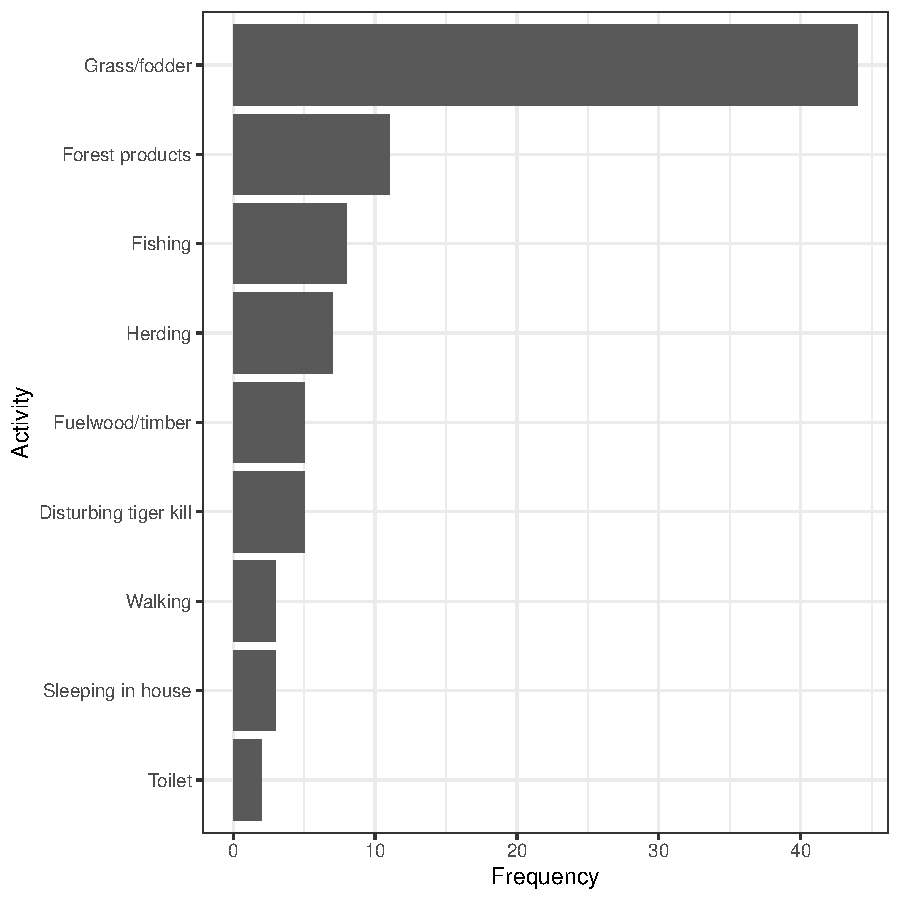
\includegraphics{BIOL202_files/figure-latex/unnamed-chunk-28-1.pdf}
\caption{\label{fig:unnamed-chunk-28}Bar graph showing the activities of 88 people at the time they were attached and killed by tigers near Chitwan national Park, Nepal, from 1979 to 2006}
\end{figure}

All figures produced using the \texttt{ggplot2} package start with the \texttt{ggplot} function. Then the following arguments:

\begin{itemize}
\tightlist
\item
  The tibble (or dataframe) that holds the data (``data = tiger.table'')
\item
  An ``aes'' argument (which stands for ``aesthetics''), within which one specifies the variables to be plotted; here we're plotting the frequencies from the ``n'' variable in the frequency table as the ``y'' variable, and the ``activity'' categorical variable as the ``x'' variable. To ensure the proper sorting of the bars, we use the \texttt{reorder} function, telling R to reorder the \texttt{activity} categories according to the frequencies in the \texttt{n} variable
\item
  Then there's a plus sign (``+'') to tell the \texttt{ggplot} function we're not done yet with our graph - there are more lines of code coming (think of it as ggplot's version of the ``pipe'')
\item
  Then the type of graph, which uses a function starting with ``geom''; here we want a bar graph, hence \texttt{geom\_bar}
\item
  The \texttt{geom\_bar} function has its own argument: ``stat = `identity'\,'' tells it just to make the height of the bars equal to the values provided in the ``y'' variable, here \texttt{n}.
\item
  The \texttt{ylab} function sets the y-axis label
\item
  The \texttt{xlab} function sets the x-axis label
\item
  The \texttt{coord\_flip} function tells it to rotate the graph horizontally; this makes it easier to fit the activity labels on the graph
\item
  Then the \texttt{theme\_bw} function indicates we want a simple black-and-white theme
\end{itemize}

There you have it: a nicely formatted bar graph!

\textbf{REMINDER} Don't forget to include a good figure caption! Here's a snapshot of the full code chunk that produced the bar graph above:

\begin{figure}
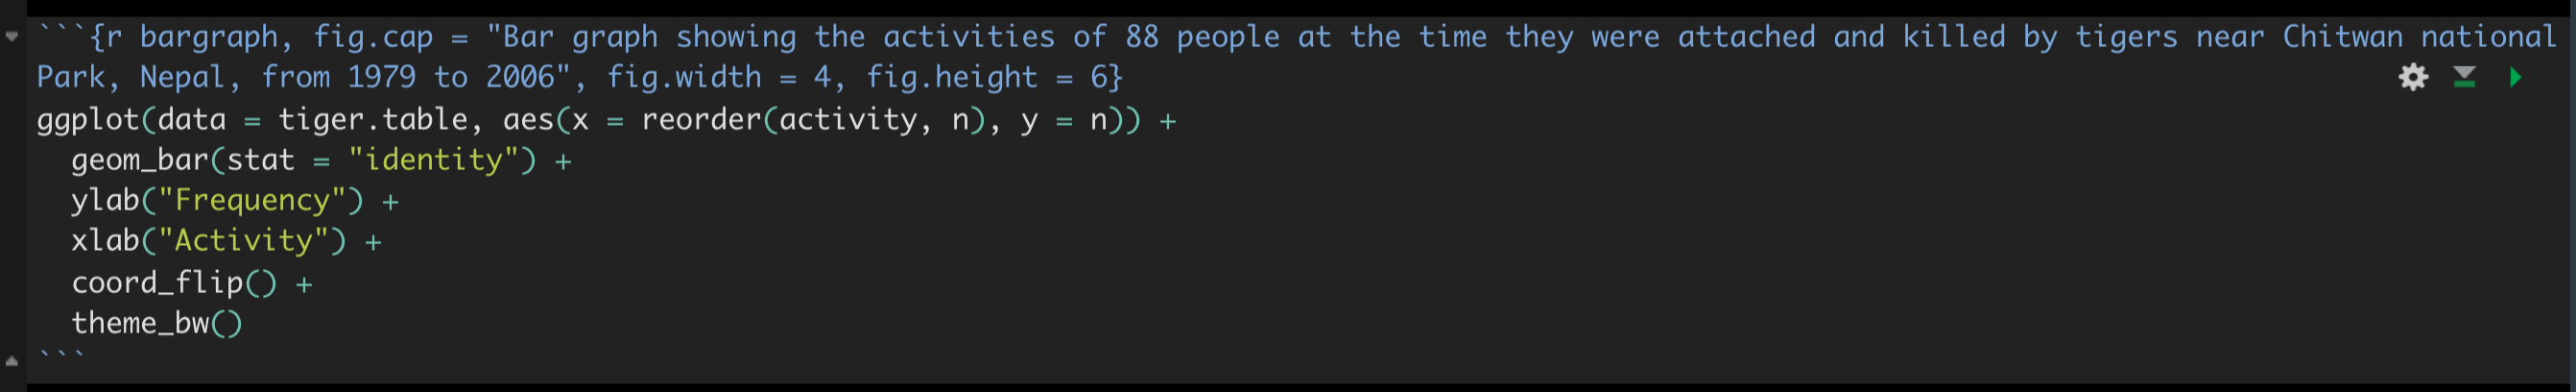
\includegraphics[width=32.69in]{./more/bar_graph_chunk} \caption{Example code chunk for producing a good bar graph}\label{fig:unnamed-chunk-29}
\end{figure}

\begin{enumerate}
\def\labelenumi{\arabic{enumi}.}
\setcounter{enumi}{2}
\tightlist
\item
  \textbf{Bar graph}: Try creating a bar graph using the \texttt{birds} dataset, which includes data about four types of birds observed at a wetland.
\end{enumerate}

\section{Create a histogram}\label{vis_histogram}

A \textbf{histogram} uses the area of rectangular bars to display the frequency distribution (or relative frequency distribution) of a numerical variable.

We'll use \texttt{ggplot} to create a histogram, and we'll again use the \texttt{penguins} dataset.

We'll give the code first, then explain below:

\begin{Shaded}
\begin{Highlighting}[]
\FunctionTok{ggplot}\NormalTok{(}\AttributeTok{data =}\NormalTok{ penguins, }\FunctionTok{aes}\NormalTok{(}\AttributeTok{x =}\NormalTok{ body\_mass\_g)) }\SpecialCharTok{+}
  \FunctionTok{geom\_histogram}\NormalTok{(}\AttributeTok{colour =} \StringTok{"black"}\NormalTok{, }\AttributeTok{fill =} \StringTok{"lightgrey"}\NormalTok{) }\SpecialCharTok{+}
  \FunctionTok{xlab}\NormalTok{(}\StringTok{"Body mass (g)"}\NormalTok{) }\SpecialCharTok{+}
  \FunctionTok{ylab}\NormalTok{(}\StringTok{"Frequency"}\NormalTok{) }\SpecialCharTok{+}
  \FunctionTok{theme\_bw}\NormalTok{()}
\end{Highlighting}
\end{Shaded}

\begin{verbatim}
## `stat_bin()` using `bins = 30`. Pick better value with `binwidth`.
\end{verbatim}

\begin{figure}
\centering
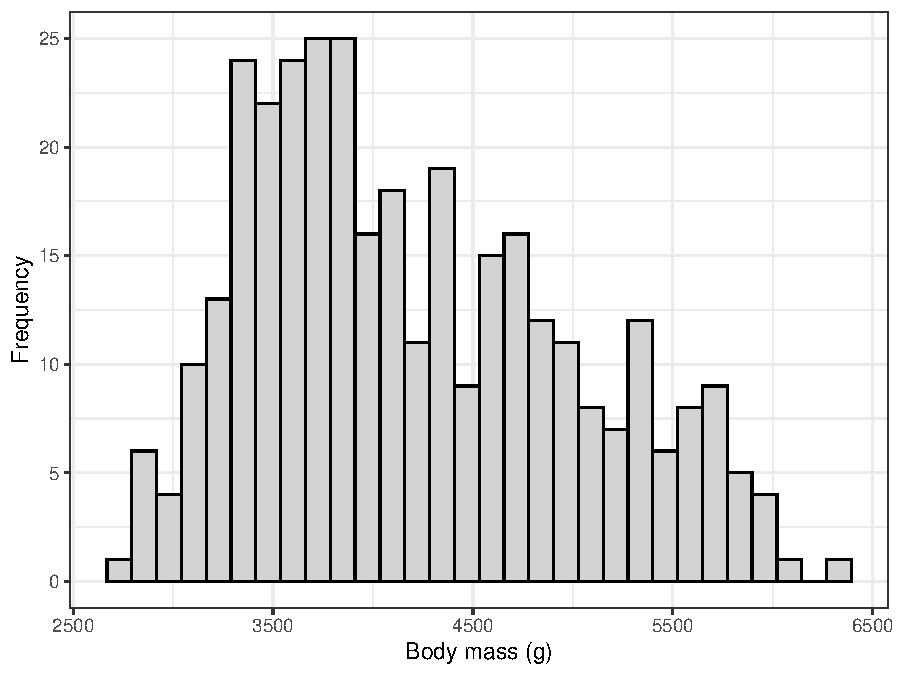
\includegraphics{BIOL202_files/figure-latex/unnamed-chunk-30-1.pdf}
\caption{\label{fig:unnamed-chunk-30}Histogram of body mass (g) for 342 penguins}
\end{figure}

The syntax follows what was seen above when creating a bar graph, but:

\begin{itemize}
\tightlist
\item
  Here we have only a single variable ``x'' variable, \texttt{body\_mass\_g} to provide the \texttt{aes} function.
\item
  We use the \texttt{geom\_histogram} function, which has its own optional arguments:

  \begin{itemize}
  \tightlist
  \item
    the ``color'' we want the outlines of each bar in the histogram to be
  \item
    the ``fill'' colour we want the bars to be
  \end{itemize}
\end{itemize}

You can also specify the ``bin width'' that \texttt{geom\_histogram} uses when generating the histogram. Notice above that we got a message stating:

\begin{verbatim}
## `stat_bin()` using `bins = 30`. Pick better value with `binwidth`.
\end{verbatim}

It's telling us that there's probably a better bin width to use. The trick is to not have to small a bin width, such that you end up with too many bars in your histogram (giving too much detail in the frequency distribution), and to not have too large a bin width such that you have too few bars in your histogram (giving too little detail).

The \texttt{hist} function that comes with base R (so no need to load a package) has an algorithm that typically chooses good bin widths. To remove some of the subjectivity from this procedure, let's leverage that function to figure out the best bin widths.

We'll provide the code then explain after:

\begin{Shaded}
\begin{Highlighting}[]
\NormalTok{penguins.hist.info }\OtherTok{\textless{}{-}} \FunctionTok{hist}\NormalTok{(penguins}\SpecialCharTok{$}\NormalTok{body\_mass\_g, }\AttributeTok{plot =} \ConstantTok{FALSE}\NormalTok{)}
\end{Highlighting}
\end{Shaded}

In the chunk above, we have:

\begin{itemize}
\tightlist
\item
  The ``penguins.hist.info'' is the name we'll give to the object we're going to create, and the assignment operator ``\textless-'' is telling R to put whatever the output from the function is into that new object
\item
  The \texttt{hist} function takes the variable you want to generate a histogram function for. And in this case, it's the \texttt{body\_mass\_g} variable in the \texttt{penguins} tibble.
\item
  The dollar sign allows you to specify the tibble name along with the variable name: ``penguins\$body\_mass\_g''.
\item
  The ``plot = FALSE'' tells the function we don't wish to produce the actual histogram, and as a consequence the function instead gives us the information that would have gone into creating the histogram, including for example the break points for the histogram bins. It packages this information in the form of a ``list'', which is one type of object.
\end{itemize}

Let's look at the info stored in the list object:

\begin{Shaded}
\begin{Highlighting}[]
\NormalTok{penguins.hist.info}
\end{Highlighting}
\end{Shaded}

\begin{verbatim}
## $breaks
## [1] 2500 3000 3500 4000 4500 5000 5500 6000 6500
## 
## $counts
## [1] 11 67 92 57 54 33 26  2
## 
## $density
## [1] 6.432749e-05 3.918129e-04 5.380117e-04 3.333333e-04 3.157895e-04
## [6] 1.929825e-04 1.520468e-04 1.169591e-05
## 
## $mids
## [1] 2750 3250 3750 4250 4750 5250 5750 6250
## 
## $xname
## [1] "penguins$body_mass_g"
## 
## $equidist
## [1] TRUE
## 
## attr(,"class")
## [1] "histogram"
\end{verbatim}

We won't worry about all the information provided here. Instead just notice that the first variable in the list is ``breaks''. Specifically, this provides us all the ``break points'' for the histogram for the given variable; break points are the values that delimit the bins for the histogram bars.

That's the information we can use to get the ideal bin width: the difference between consecutive breaks is our desired bin width!

In this example it's easy to see that the bin width was 500. But lets provide code to calculate it and thus make sure it's reproducible. We simply need to calculate the difference between any two consecutive break points (they will all be equal in magnitude):

\begin{Shaded}
\begin{Highlighting}[]
\NormalTok{penguins.hist.info}\SpecialCharTok{$}\NormalTok{breaks[}\DecValTok{2}\NormalTok{] }\SpecialCharTok{{-}}\NormalTok{ penguins.hist.info}\SpecialCharTok{$}\NormalTok{breaks[}\DecValTok{1}\NormalTok{]}
\end{Highlighting}
\end{Shaded}

\begin{verbatim}
## [1] 500
\end{verbatim}

The above code simply asks R to calculate the difference (using the subtraction sign) between the second element of the ``breaks'' variable, denoted using the square brackets ``breaks{[}2{]}'', and the first element ``breaks{[}2{]}''.

And R returns 500. That's the bin width we want to use!

So let's edit the original histogram code to include the ``binwidth'' argument in the \texttt{geom\_histogram} function, as follows:

\begin{Shaded}
\begin{Highlighting}[]
\FunctionTok{ggplot}\NormalTok{(}\AttributeTok{data =}\NormalTok{ penguins, }\FunctionTok{aes}\NormalTok{(}\AttributeTok{x =}\NormalTok{ body\_mass\_g)) }\SpecialCharTok{+}
  \FunctionTok{geom\_histogram}\NormalTok{(}\AttributeTok{binwidth =} \DecValTok{500}\NormalTok{, }\AttributeTok{colour =} \StringTok{"black"}\NormalTok{, }\AttributeTok{fill =} \StringTok{"lightgrey"}\NormalTok{) }\SpecialCharTok{+}
  \FunctionTok{xlab}\NormalTok{(}\StringTok{"Body mass (g)"}\NormalTok{) }\SpecialCharTok{+}
  \FunctionTok{ylab}\NormalTok{(}\StringTok{"Frequency"}\NormalTok{) }\SpecialCharTok{+}
  \FunctionTok{theme\_bw}\NormalTok{()}
\end{Highlighting}
\end{Shaded}

\begin{figure}
\centering
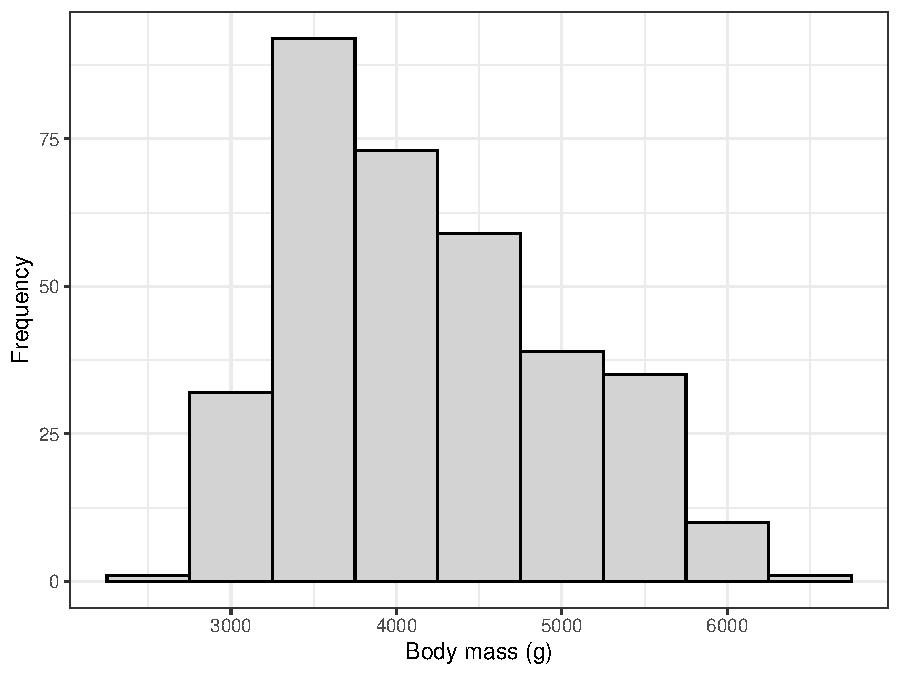
\includegraphics{BIOL202_files/figure-latex/unnamed-chunk-31-1.pdf}
\caption{\label{fig:unnamed-chunk-31}Histogram of body mass (g) for 342 penguins}
\end{figure}

There we go! Now we need to learn how to describe and interpret a histogram\ldots{}

\section{Describing a histogram}\label{vis_describe_hist}

Things to note in your description of a histogram:

\begin{itemize}
\tightlist
\item
  Is it roughly symmetric or is it negatively or positively skewed?
\item
  Is it roughly bell-shaped?
\item
  Outliers - are there observations (bars) showing up far from the others?
\item
  Are there multiple modes?
\end{itemize}

So, let's look again at the penguin body mass histogram, and provide a description thereafter:

\begin{Shaded}
\begin{Highlighting}[]
\FunctionTok{ggplot}\NormalTok{(}\AttributeTok{data =}\NormalTok{ penguins, }\FunctionTok{aes}\NormalTok{(}\AttributeTok{x =}\NormalTok{ body\_mass\_g)) }\SpecialCharTok{+}
  \FunctionTok{geom\_histogram}\NormalTok{(}\AttributeTok{binwidth =} \DecValTok{500}\NormalTok{, }\AttributeTok{colour =} \StringTok{"black"}\NormalTok{, }\AttributeTok{fill =} \StringTok{"lightgrey"}\NormalTok{) }\SpecialCharTok{+}
  \FunctionTok{xlab}\NormalTok{(}\StringTok{"Body mass (g)"}\NormalTok{) }\SpecialCharTok{+}
  \FunctionTok{ylab}\NormalTok{(}\StringTok{"Frequency"}\NormalTok{) }\SpecialCharTok{+}
  \FunctionTok{theme\_bw}\NormalTok{()}
\end{Highlighting}
\end{Shaded}

\begin{figure}
\centering
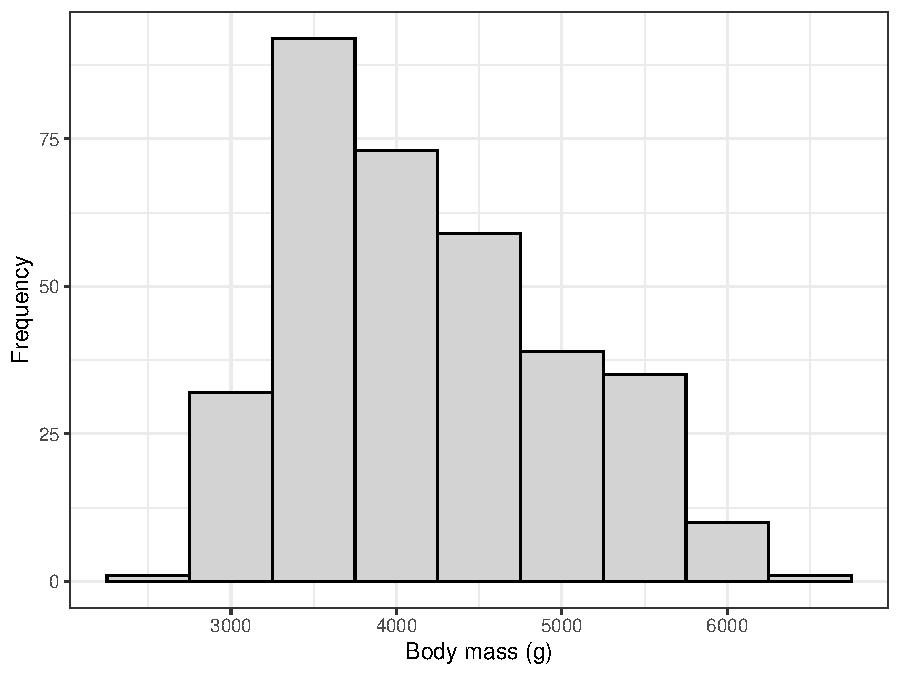
\includegraphics{BIOL202_files/figure-latex/unnamed-chunk-32-1.pdf}
\caption{\label{fig:unnamed-chunk-32}Histogram of body mass (g) for 342 penguins}
\end{figure}

The histogram is moderately positively skewed and thus asymmetric, with a single mode near 3500g. There are no obvious outliers in the distribution.

\begin{enumerate}
\def\labelenumi{\arabic{enumi}.}
\tightlist
\item
  \textbf{Histogram}: Create a histogram of the bill lengths of penguins in the \texttt{penguins} dataset, and include an appropriate figure caption. Then provide a description of what you see.
\end{enumerate}

\chapter{Describing a single variable}\label{vis_describe}

\textbf{Tutorial learning objectives}

In this tutorial you will:

\begin{itemize}
\tightlist
\item
  Learn how to calculate the main descriptor of a categorical variable: the \textbf{proportion}
\item
  Learn how to calculate measures of centre and spread for a single numerical variable
\end{itemize}

\section{Load packages and import data}\label{desc_packages_data}

Let's load some packages first:

\begin{Shaded}
\begin{Highlighting}[]
\FunctionTok{library}\NormalTok{(tidyverse)}
\FunctionTok{library}\NormalTok{(palmerpenguins)}
\FunctionTok{library}\NormalTok{(skimr)}
\FunctionTok{library}\NormalTok{(knitr)}
\FunctionTok{library}\NormalTok{(janitor)}
\end{Highlighting}
\end{Shaded}

And we're introducing a new package called \texttt{naniar}, which helps us deal more easily with missing values in datasets.

You may need to install that package (\textbf{recall} you only do this once!). Consult a \hyperref[package_install]{previous tutorial} if you forget how.

Once you've installed it, load it:

\begin{Shaded}
\begin{Highlighting}[]
\FunctionTok{library}\NormalTok{(naniar)}
\end{Highlighting}
\end{Shaded}

We will use the following datasets in this tutorial:

\begin{itemize}
\tightlist
\item
  the \texttt{birds.csv} file contains counts of different categories of bird observed at a marsh habitat
\item
  the \texttt{penguins} dataset that is available as part of the \texttt{palmerpenguins} package
\end{itemize}

\begin{Shaded}
\begin{Highlighting}[]
\NormalTok{birds }\OtherTok{\textless{}{-}} \FunctionTok{read\_csv}\NormalTok{(}\StringTok{"https://raw.githubusercontent.com/ubco{-}biology/BIOL202/main/data/birds.csv"}\NormalTok{)}
\end{Highlighting}
\end{Shaded}

\begin{verbatim}
## Rows: 86 Columns: 1
## -- Column specification --------------------------------------------------------
## Delimiter: ","
## chr (1): type
## 
## i Use `spec()` to retrieve the full column specification for this data.
## i Specify the column types or set `show_col_types = FALSE` to quiet this message.
\end{verbatim}

\section{Describing a categorical variable}\label{desc_cat_Var}

The \emph{proportion} is the most important descriptive statistic for a categorical variable. It measures the fraction of observations in a given category within a categorical variable.

For example, the \texttt{birds.csv} file has a single variable called \texttt{type} that includes tallies (frequencies) of each of four categories of bird observed at a marsh habitat.

\begin{Shaded}
\begin{Highlighting}[]
\NormalTok{birds}
\end{Highlighting}
\end{Shaded}

\begin{verbatim}
## # A tibble: 86 x 1
##    type     
##    <chr>    
##  1 Waterfowl
##  2 Predatory
##  3 Predatory
##  4 Waterfowl
##  5 Shorebird
##  6 Waterfowl
##  7 Waterfowl
##  8 Songbird 
##  9 Predatory
## 10 Waterfowl
## # i 76 more rows
\end{verbatim}

The \emph{proportion} of birds belonging to a given category is the same as the \emph{relative frequency} of birds belonging to a given category.

In a previous \hyperref[vis_cat_freq_table]{tutorial}, using the \texttt{tigerdeaths} dataset, we learned how to create a frequency table that included relative frequencies.

Let's use the same approach for the \texttt{birds} dataset. First we create the frequency table, then we display the table with an appropriate heading:

\begin{Shaded}
\begin{Highlighting}[]
\NormalTok{birds.table }\OtherTok{\textless{}{-}}\NormalTok{ birds }\SpecialCharTok{\%\textgreater{}\%}
  \FunctionTok{count}\NormalTok{(type, }\AttributeTok{sort =} \ConstantTok{TRUE}\NormalTok{) }\SpecialCharTok{\%\textgreater{}\%} 
  \FunctionTok{mutate}\NormalTok{(}\AttributeTok{relative\_frequency =}\NormalTok{ n }\SpecialCharTok{/} \FunctionTok{sum}\NormalTok{(n)) }\SpecialCharTok{\%\textgreater{}\%} 
  \FunctionTok{adorn\_totals}\NormalTok{()}
\end{Highlighting}
\end{Shaded}

\textbf{NOTE}
If there are missing values (``NA'') in the categorical variable, the preceding code will successfully enumerate those and create an ``NA'' category in the frequency table.

Now display the table:

\begin{Shaded}
\begin{Highlighting}[]
\NormalTok{birds.table }\SpecialCharTok{\%\textgreater{}\%}
  \FunctionTok{kable}\NormalTok{(}\AttributeTok{caption =} \StringTok{"Frequency table showing the frequencies of each of four types of bird observed at a marsh habitat (N = 86)"}\NormalTok{, }\AttributeTok{digits =} \DecValTok{3}\NormalTok{)}
\end{Highlighting}
\end{Shaded}

\label{tab:birdfreqtable}Frequency table showing the frequencies of each of four types of bird observed at a marsh habitat (N = 86)

type

n

relative\_frequency

Waterfowl

43

0.500

Predatory

29

0.337

Shorebird

8

0.093

Songbird

6

0.070

Total

86

1.000

We can see, for example, that the proportion (relative frequency) of birds belonging to the ``Predatory'' category was 0.3372093.

We calculate proportions (relative frequencies) using the simple formula:

\[\hat{p} = \frac{n_i}{N}\]
Where \[n_i\] is the frequency of observations in the given category of interest \emph{i}, and \emph{N} is total number of observations (sample size) across all categories.

\textbf{Reminder}
Proportions, and thus relative frequencies, must be between 0 and 1.

\section{Describing a numerical variable}\label{desc_numeric_var}

Numeric variables are described with measures of \textbf{centre} and \textbf{spread}.

Before calculating descriptive statistics for a numeric variable, it is advisable to visualize its frequency distribution first. Why? Because characteristics of the frequency distribution will govern which measures of centre and spread are more reliable or representative.

\begin{itemize}
\item
  If the frequency distribution is roughly symmetric and does not have any obvious outliers, then the \textbf{mean} and the \textbf{standard deviation} are the preferred measures of centre and spread, respectively
\item
  If the frequency distribution is asymmetric and / or has outliers, the \textbf{median} and the \textbf{inter-quartile range} (IQR) are the preferred measures of centre and spread
\end{itemize}

It is often the case, however, that all four measures are presented together.

\textbf{New tool}
Introducing the \texttt{summarise} function.

The \texttt{dplyr} package, which is loaded with the \texttt{tidyverse}, has a handy \texttt{summarise} (equivalently \texttt{summarize}) function for calculating descriptive statistics.

Check out its help file by copying the following code into your command console:

\begin{verbatim}
?summarise
\end{verbatim}

Let's use the \texttt{penguins} dataset for our demonstrations.

The first step is to visualize the frequency distribution. Given that this is a numeric variable, we do this using a histogram, as we learned in a previous \hyperref[vis_histogram]{tutorial}.

\begin{Shaded}
\begin{Highlighting}[]
\FunctionTok{ggplot}\NormalTok{(}\AttributeTok{data =}\NormalTok{ penguins, }\FunctionTok{aes}\NormalTok{(}\AttributeTok{x =}\NormalTok{ body\_mass\_g)) }\SpecialCharTok{+}
  \FunctionTok{geom\_histogram}\NormalTok{(}\AttributeTok{binwidth =} \DecValTok{500}\NormalTok{, }\AttributeTok{colour =} \StringTok{"black"}\NormalTok{, }\AttributeTok{fill =} \StringTok{"lightgrey"}\NormalTok{) }\SpecialCharTok{+}
  \FunctionTok{xlab}\NormalTok{(}\StringTok{"Body mass (g)"}\NormalTok{) }\SpecialCharTok{+}
  \FunctionTok{ylab}\NormalTok{(}\StringTok{"Frequency"}\NormalTok{) }\SpecialCharTok{+}
  \FunctionTok{theme\_bw}\NormalTok{()}
\end{Highlighting}
\end{Shaded}

\begin{figure}
\centering
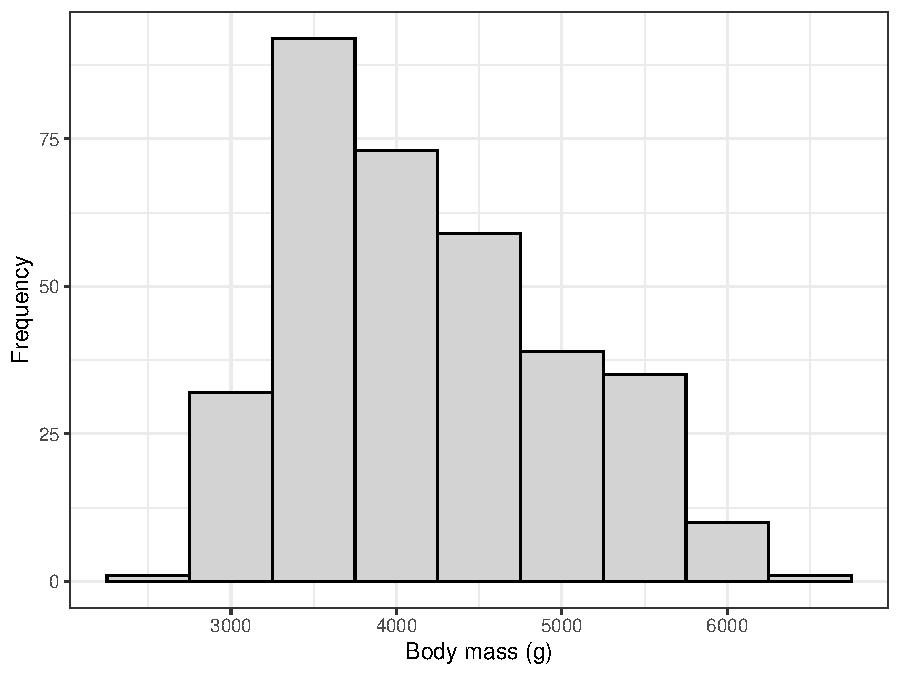
\includegraphics{BIOL202_files/figure-latex/unnamed-chunk-34-1.pdf}
\caption{\label{fig:unnamed-chunk-34}Histogram of body mass (g) for 342 penguins}
\end{figure}

We are reminded that the distribution of body mass is moderately positively skewed and thus asymmetric, with a single mode near 3500g. There are no obvious outliers in the distribution.

This means that the \textbf{median} and \textbf{IQR} should be the preferred descriptors of centre and spread, respectively.

\subsection{Calculating the median \& IQR}\label{median_IQR}

So let's calculate the median and IQR of body mass for all penguins. Let's provide the code, then explain after:

\begin{verbatim}
penguins %>%
  summarise(
   median_body_mass_g =  median(body_mass_g),
   IQR_body_mass_g = IQR(body_mass_g)
    )
\end{verbatim}

Uh oh! If you tried to run this code, it would have given you an error:

\begin{figure}
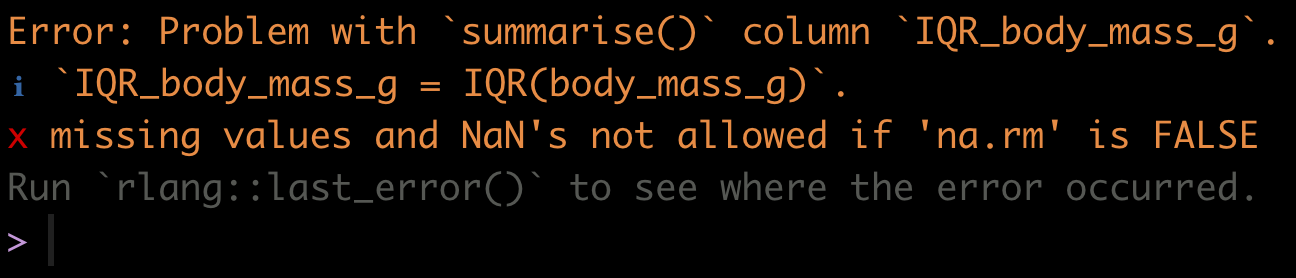
\includegraphics[width=18in]{./more/na_error} \caption{Error when functions encounter 'NA' values}\label{fig:unnamed-chunk-35}
\end{figure}

We forgot that when we \hyperref[vis_data_overview]{previously} got an overview of the \texttt{penguins} dataset we discovered there were missing values (``NA'' values)!

\textbf{TIP}
If there are ``NA'' values in the variable being analyzed, some R functions, such as the function \texttt{median} or \texttt{mean}, will simply return ``NA''. To remedy this, we use the ``na.rm = TRUE'' argument.

Let's try our code again, adding the ``na.rm = TRUE'' argument. And note that the key functions called within the \texttt{summarise} function are \texttt{median} and \texttt{IQR} (case sensitive!).

\begin{Shaded}
\begin{Highlighting}[]
\NormalTok{penguins }\SpecialCharTok{\%\textgreater{}\%}
  \FunctionTok{summarise}\NormalTok{(}
   \AttributeTok{Median =}  \FunctionTok{median}\NormalTok{(body\_mass\_g, }\AttributeTok{na.rm =} \ConstantTok{TRUE}\NormalTok{),}
   \AttributeTok{InterQR =} \FunctionTok{IQR}\NormalTok{(body\_mass\_g, }\AttributeTok{na.rm =} \ConstantTok{TRUE}\NormalTok{)}
\NormalTok{    )}
\end{Highlighting}
\end{Shaded}

\begin{verbatim}
## # A tibble: 1 x 2
##   Median InterQR
##    <dbl>   <dbl>
## 1   4050    1200
\end{verbatim}

In the preceding code chunk, we have:

\begin{itemize}
\tightlist
\item
  The name of the tibble (here \texttt{penguins}) being used in the subsequent functions
\item
  A pipe ``\%\textgreater\% to tell R we're not done coding
\item
  The \texttt{summarise} function (\texttt{summarize} will work too), telling R we're going to calculate a new variable
\item
  The name we'll give to the first variable we're creating, here we call the variable ``Median'' (the ``M'' is capitalized to distinguish this variable name from the function \texttt{median})
\item
  And we define how to calculate the ``Median'', here using the \texttt{median} function
\item
  We feed the variable of interest from the \texttt{penguins} tibble, ``body\_mass\_g'', to the \texttt{median} function, along with the argument ``na.rm = TRUE''
\item
  We end the line with a comma, telling R that we're not done providing arguments to the \texttt{summarise} function
\item
  We do the same for the inter-quartile range variable we're creating called ``InterQR'', calculating the value using the \texttt{IQR} function, and this time no comma at the end of the line, because this is the last argument being provided to the \texttt{summarise} function
\item
  We close out the parentheses for the \texttt{summarise} function
\end{itemize}

\subsection{Calculating the mean \& standard deviation}\label{mean_sd}

Although the median and IQR are the preferred descriptors for the \texttt{body\_mass\_g} variable, it is nonetheless commonplace to report the mean and standard deviation also.

Let's do this, and while we're at it, include even more descriptors to illustrate how they're calculated.

This time we'll put the output from our \texttt{summarise} function into a table, and then present it in a nice format, like we learned how to do for a \hyperref[vis_cat_freq_table]{frequency table}.

Let's create the table of descriptive statistics first, a tibble called ``penguins.descriptors'', and we'll describe what's going on after (\textbf{NOTE} this code chunk was edited slightly on Sept.~30, 2021):

\begin{Shaded}
\begin{Highlighting}[]
\NormalTok{penguins.descriptors }\OtherTok{\textless{}{-}}\NormalTok{ penguins }\SpecialCharTok{\%\textgreater{}\%}
  \FunctionTok{summarise}\NormalTok{( }
  \AttributeTok{Mean =} \FunctionTok{mean}\NormalTok{(body\_mass\_g, }\AttributeTok{na.rm =}\NormalTok{ T),}
  \AttributeTok{SD =} \FunctionTok{sd}\NormalTok{(body\_mass\_g, }\AttributeTok{na.rm =}\NormalTok{ T),}
  \AttributeTok{Median =} \FunctionTok{median}\NormalTok{(body\_mass\_g, }\AttributeTok{na.rm =}\NormalTok{ T),}
  \AttributeTok{InterQR =} \FunctionTok{IQR}\NormalTok{(body\_mass\_g, }\AttributeTok{na.rm =}\NormalTok{ T),}
  \AttributeTok{Count =} \FunctionTok{n}\NormalTok{() }\SpecialCharTok{{-}}\NormalTok{ naniar}\SpecialCharTok{::}\FunctionTok{n\_miss}\NormalTok{(body\_mass\_g),}
  \AttributeTok{Count\_NA =}\NormalTok{ naniar}\SpecialCharTok{::}\FunctionTok{n\_miss}\NormalTok{(body\_mass\_g))}
\end{Highlighting}
\end{Shaded}

The first 4 descriptive statistics are self-explanatory based on their variable names.

The last two: ``Count'' and ``Count\_NA'' are providing the total number of complete observations in the \texttt{body\_mass\_g} variable (thus the number of observations that went into calculating the descriptive statistics), and then the total number of missing values (NAs) in the variable, respectively.

The last two lines of code above require further explanation:

This code: \texttt{Count\ =\ n()\ -\ naniar::n\_miss(body\_mass\_g))} tells R to first tally the total sample size using the \texttt{n()} function, then to subtract from that the total number of missing values, which is calculated using the \texttt{n\_miss} function from the \texttt{naniar} package.

The double colons in \texttt{naniar::n\_miss(body\_mass\_g)} indicates that the function \texttt{n\_miss} comes from the \texttt{naniar} package. This syntax, which we have not used previously, provides a failsafe way to run a function even if the package is not presently loaded.

The same coding approach is used in the last line: \texttt{Count\_NA\ =\ naniar::n\_miss(body\_mass\_g)}.

\begin{center}\rule{0.5\linewidth}{0.5pt}\end{center}

\textbf{TIP}
It is important to calculate the total number of complete observations in the variable of interest, because, as described in the \href{https://ubco-biology.github.io/Procedures-and-Guidelines/figures-tables.html}{Biology Procedures and Guidelines document}, this number needs to be reported in figure and table headings.

Now let's show the table of descriptive statistics, using the \texttt{kable} function we learned about in a previous tutorial.

\begin{Shaded}
\begin{Highlighting}[]
\NormalTok{penguins.descriptors }\SpecialCharTok{\%\textgreater{}\%}
  \FunctionTok{kable}\NormalTok{(}\AttributeTok{caption =} \StringTok{"Descriptive statistics of measurements of body mass (g) for 342 penguins"}\NormalTok{, }\AttributeTok{digits =} \DecValTok{3}\NormalTok{)}
\end{Highlighting}
\end{Shaded}

\label{tab:penguindescribe}Descriptive statistics of measurements of body mass (g) for 342 penguins

Mean

SD

Median

InterQR

Count

Count\_NA

4201.754

801.955

4050

1200

342

2

In another tutorial we'll learn how to present the table following all the guidelines in the \href{https://ubco-biology.github.io/Procedures-and-Guidelines/figures-tables.html}{Biology Guidelines and Procedures document}, including, for example, significant digits. For now, the preceding table is good!

\begin{enumerate}
\def\labelenumi{\arabic{enumi}.}
\tightlist
\item
  \textbf{Descriptive statistics}: Create a histogram and table of descriptive statistics for the ``flipper\_length\_mm'' variable in the \texttt{penguins} dataset.
\end{enumerate}

\section{Describing a numerical variable grouped by a categorical variable}\label{desc_numeric_var_cat}

In this tutorial you'll learn how to calculate descriptive statistics for a numerical variable grouped according to categories of a categorical variable.

For example, a common scenario in biology is to want to calculate and report the mean and standard deviation of a response variable for different ``treatment groups'' in an experiment. (More commonly we would report the mean and standard error, but that's for a later tutorial!).

It is straightforward to modify the code we used in the preceding tutorial to do what we want.

Specifically, we use the \texttt{group\_by} function from the \texttt{dplyr} package to tell R to do the calculations on the observations within each category of the grouping variable.

For example, let's describe penguin body mass grouped by ``species''.

We'll create a new tibble object called ``penguins.descriptors.byspecies'', and we insert one line of code using the \texttt{group\_by} function, and telling R which categorical variable to use for the grouping (here, ``species''):

\begin{Shaded}
\begin{Highlighting}[]
\NormalTok{penguins.descriptors.byspecies }\OtherTok{\textless{}{-}}\NormalTok{ penguins }\SpecialCharTok{\%\textgreater{}\%}
  \FunctionTok{group\_by}\NormalTok{(species) }\SpecialCharTok{\%\textgreater{}\%}
\FunctionTok{summarise}\NormalTok{(}
  \AttributeTok{Mean =} \FunctionTok{mean}\NormalTok{(body\_mass\_g, }\AttributeTok{na.rm =}\NormalTok{ T),}
  \AttributeTok{SD =} \FunctionTok{sd}\NormalTok{(body\_mass\_g, }\AttributeTok{na.rm =}\NormalTok{ T),}
  \AttributeTok{Median =} \FunctionTok{median}\NormalTok{(body\_mass\_g, }\AttributeTok{na.rm =}\NormalTok{ T),}
  \AttributeTok{InterQR =} \FunctionTok{IQR}\NormalTok{(body\_mass\_g, }\AttributeTok{na.rm =}\NormalTok{ T),}
  \AttributeTok{Count =} \FunctionTok{n}\NormalTok{() }\SpecialCharTok{{-}}\NormalTok{ naniar}\SpecialCharTok{::}\FunctionTok{n\_miss}\NormalTok{(body\_mass\_g),}
  \AttributeTok{Count\_NA =}\NormalTok{ naniar}\SpecialCharTok{::}\FunctionTok{n\_miss}\NormalTok{(body\_mass\_g))}
\end{Highlighting}
\end{Shaded}

It's that simple!

Let's have a look at the output:

\begin{Shaded}
\begin{Highlighting}[]
\NormalTok{penguins.descriptors.byspecies}
\end{Highlighting}
\end{Shaded}

\begin{verbatim}
## # A tibble: 3 x 7
##   species    Mean    SD Median InterQR Count Count_NA
##   <fct>     <dbl> <dbl>  <dbl>   <dbl> <int>    <int>
## 1 Adelie    3701. 458.6   3700   650     151        1
## 2 Chinstrap 3733. 384.3   3700   462.5    68        0
## 3 Gentoo    5076. 504.1   5000   800     123        1
\end{verbatim}

\begin{enumerate}
\def\labelenumi{\arabic{enumi}.}
\tightlist
\item
  Use the \texttt{kable} function to output this new tibble in a nice format
\end{enumerate}

\chapter{Visualizing associations between two variables}\label{vis_twovar}

\textbf{Tutorial learning objectives}

In this tutorial you will:

\begin{itemize}
\tightlist
\item
  Learn how to visualize associations between two categorical variables using a contingency table
\item
  Learn how to visualize associations between two categorical variables graphically
\item
  Learn how to visualize associations between two numerical variables
\item
  Learn how to visualize associations between a numerical response variable and a categorical explanatory variable
\end{itemize}

\textbf{Background}

The type of graph that is most suitable for visualizing an association between two variables depends upon the type of data being visualized:

\begin{itemize}
\tightlist
\item
  If both variables are categorical, we can visualize the association in a table called a \textbf{contingency table}, or we can visualize the association graphically using a \textbf{grouped bar chart} or a \textbf{mosaic plot}
\item
  If both variables are numeric, we visualize the association graphically using a \textbf{scatterplot}
\item
  If the response variable is numerical and the explanatory variable is categorical, we visualize the association graphically using a \textbf{strip chart}, \textbf{boxplot}, or variations on these
\item
  We do not discuss the scenario where the response variable is categorical and the explanatory variable is numerical
\end{itemize}

In this tutorial you'll learn to construct and interpret each of these types of visualization. In later tutorials you'll learn how to conduct statistical analyses of these associations.

\section{Load packages and import data}\label{vis2_packages_data}

Let's load some familiar packages first:

\begin{Shaded}
\begin{Highlighting}[]
\FunctionTok{library}\NormalTok{(tidyverse)}
\FunctionTok{library}\NormalTok{(palmerpenguins)}
\FunctionTok{library}\NormalTok{(knitr)}
\FunctionTok{library}\NormalTok{(skimr)}
\end{Highlighting}
\end{Shaded}

We also need the \texttt{janitor} package, the \texttt{ggmosaic} package, and the \texttt{ggExtra} packages, and these are likely to be new to you. Check whether these packages are installed under the ``packages'' tab in the bottom-right panel in RStudio. If they are not yet installed, then \hyperref[package_install]{install them}. \textbf{Only install them once on your computer!}

Load the packages:

\begin{Shaded}
\begin{Highlighting}[]
\FunctionTok{library}\NormalTok{(janitor)}
\FunctionTok{library}\NormalTok{(ggmosaic)}
\FunctionTok{library}\NormalTok{(ggExtra)}
\end{Highlighting}
\end{Shaded}

\textbf{Import Data}

We'll again make use of the \texttt{penguins} dataset, which gets loaded as a ``tibble'' object with the \texttt{palmerpenguins} package.

Import the \texttt{locusts.csv} data, which are described in the Whitlock \& Schluter text, Figure 2.1-2. We'll create a tibble called \texttt{locust}.

\begin{Shaded}
\begin{Highlighting}[]
\NormalTok{locust }\OtherTok{\textless{}{-}} \FunctionTok{read\_csv}\NormalTok{(}\StringTok{"https://raw.githubusercontent.com/ubco{-}biology/BIOL202/main/data/locust.csv"}\NormalTok{)}
\end{Highlighting}
\end{Shaded}

\begin{verbatim}
## Rows: 30 Columns: 2
## -- Column specification --------------------------------------------------------
## Delimiter: ","
## dbl (2): serotoninLevel, treatmentTime
## 
## i Use `spec()` to retrieve the full column specification for this data.
## i Specify the column types or set `show_col_types = FALSE` to quiet this message.
\end{verbatim}

Import the \texttt{bird.malaria.csv} data, which are described in the Whitlock \& Schluter text, Example 2.3A (p.~40). We'll create a tibble called \texttt{bird.malaria}.

\begin{Shaded}
\begin{Highlighting}[]
\NormalTok{bird.malaria}\OtherTok{\textless{}{-}} \FunctionTok{read\_csv}\NormalTok{(}\StringTok{"https://raw.githubusercontent.com/ubco{-}biology/BIOL202/main/data/bird\_malaria.csv"}\NormalTok{)}
\end{Highlighting}
\end{Shaded}

\begin{verbatim}
## Rows: 65 Columns: 3
## -- Column specification --------------------------------------------------------
## Delimiter: ","
## chr (2): treatment, response
## dbl (1): bird
## 
## i Use `spec()` to retrieve the full column specification for this data.
## i Specify the column types or set `show_col_types = FALSE` to quiet this message.
\end{verbatim}

\begin{enumerate}
\def\labelenumi{\arabic{enumi}.}
\tightlist
\item
  Get an overview of the \texttt{locust} and \texttt{bird.malaria} tibbles.
\end{enumerate}

\section{Visualizing association between two categorical variables}\label{vis2_2cat}

We'll cover three ways to visualize associations between two categorical variables:

\begin{itemize}
\tightlist
\item
  a \textbf{contingency table}
\item
  a \textbf{grouped bar graph}
\item
  a \textbf{mosaic plot}
\end{itemize}

\subsection{Constructing a contingency table}\label{vis2_cont_table}

\textbf{New tool}
The \texttt{tabyl} function from the \texttt{janitor} package is useful for creating contingency tables, or more generally, cross-tabulating frequencies for multiple categorical variables.

You can check out more about the \texttt{tabyl} function at this \href{https://cran.r-project.org/web/packages/janitor/vignettes/tabyls.html}{vignette}.

Let's use the \texttt{bird.malaria} dataset for our demonstration.

If you got an overview of the dataset, as suggested as part of the activity in the preceding section, you would have seen that the \texttt{bird.malaria} tibble includes two categorical variables: \texttt{treatment} and \texttt{response}, each with 2 categories.

The dataset includes 65 rows. Each row corresponds to an individual (unique) bird. Thirty of the birds were randomly assigned to the ``Control'' treatment group, and 35 were randomly assigned to the ``Egg removal'' treatment group.

The \texttt{response} variable includes the categories ``Malaria'' and ``No Malaria'', indicating whether the bird contracted Malaria after the treatment.

Our goal is to visualize the frequency of birds that fall into each of the four unique combinations of category:

\begin{itemize}
\tightlist
\item
  Control + No Malaria
\item
  Control + Malaria
\item
  Egg removal + No Malaria
\item
  Egg removal + Malaria
\end{itemize}

More specifically, we are interested in comparing the incidence of malaria among the Control and Egg removal treatment groups. We'll learn in a later tutorial how to conduct this comparison statistically.

Let's provide the code, then explain after. We'll again make use of the \texttt{kable} function from the \texttt{knitr} package to help present a nice table. So first we create the table (``bird.malaria.table''), then in a later code chunk we'll output a nice version of the table using the \texttt{kable} function.

First create the basic contingency table:

\begin{Shaded}
\begin{Highlighting}[]
\NormalTok{bird.malaria.freq }\OtherTok{\textless{}{-}}\NormalTok{ bird.malaria }\SpecialCharTok{\%\textgreater{}\%}
  \FunctionTok{tabyl}\NormalTok{(treatment, response)}
\end{Highlighting}
\end{Shaded}

Code explanation:

\begin{itemize}
\tightlist
\item
  the first line is telling R to assign any output from our commands to the object called ``bird.malaria.freq''
\item
  the first line is also telling R that we're using the \texttt{bird.malaria} object as input to our subsequent functions, and the pipe (\%\textgreater\%) tells R there's more to come.
\item
  the second line uses the \texttt{tabyl} function, and we provide it with the names of the variables from the \texttt{bird.malaria} object that we want to use for tabulating frequencies. Here we provide the variable names ``treatment'', and ``response''
\end{itemize}

Let's look at the table:

\begin{Shaded}
\begin{Highlighting}[]
\NormalTok{bird.malaria.freq}
\end{Highlighting}
\end{Shaded}

\begin{verbatim}
##    treatment Malaria No Malaria
##      Control       7         28
##  Egg removal      15         15
\end{verbatim}

It is typically a good idea to also include the row and column totals in a contingency table.

To do this, we use the \texttt{adorn\_totals} function, from the \texttt{janitor} package, as follows, and we'll create a new object called ``bird.malaria.freq.totals'':

\begin{Shaded}
\begin{Highlighting}[]
\NormalTok{bird.malaria.freq.totals }\OtherTok{\textless{}{-}}\NormalTok{ bird.malaria }\SpecialCharTok{\%\textgreater{}\%}
  \FunctionTok{tabyl}\NormalTok{(treatment, response) }\SpecialCharTok{\%\textgreater{}\%}
  \FunctionTok{adorn\_totals}\NormalTok{(}\AttributeTok{where =} \FunctionTok{c}\NormalTok{(}\StringTok{"row"}\NormalTok{, }\StringTok{"col"}\NormalTok{))}
\end{Highlighting}
\end{Shaded}

\begin{itemize}
\tightlist
\item
  the last line tells the \texttt{adorn\_totals} function that we want to add the row and column totals to our table
\end{itemize}

Now let's see what the table looks like before using the \texttt{kable} function. To do this, just provide the name of the object:

\begin{Shaded}
\begin{Highlighting}[]
\NormalTok{bird.malaria.freq.totals}
\end{Highlighting}
\end{Shaded}

\begin{verbatim}
##    treatment Malaria No Malaria Total
##      Control       7         28    35
##  Egg removal      15         15    30
##        Total      22         43    65
\end{verbatim}

Now let's use the \texttt{kable} function to improve the look, and add a table heading.

\begin{Shaded}
\begin{Highlighting}[]
\NormalTok{bird.malaria.freq.totals }\SpecialCharTok{\%\textgreater{}\%}
  \FunctionTok{kable}\NormalTok{(}\AttributeTok{caption =} \StringTok{"Contingency table showing the incidence of malaria in female great tits in relation to experimental treatment"}\NormalTok{, }\AttributeTok{booktabs =} \ConstantTok{TRUE}\NormalTok{)}
\end{Highlighting}
\end{Shaded}

\label{tab:vismalaria}Contingency table showing the incidence of malaria in female great tits in relation to experimental treatment

treatment

Malaria

No Malaria

Total

Control

7

28

35

Egg removal

15

15

30

Total

22

43

65

\textbf{Relative frequencies}

Often it is useful to also present a contingency table that shows the \emph{relative frequencies}. However, it's important to know how to calculate those relative frequencies.

For instance, recall that in this malaria example, we are interested in comparing the incidence of malaria among the Control and Egg removal treatment groups. Thus, we should calculate the relative frequencies using the \textbf{row totals}. This will become clear when we show the table.

We can get relative frequencies, which are equivalent to proportions, using the \texttt{adorn\_percentages} function (the function name is a misnomer, because we're calculating proportions, not percentages!), and telling R to use the row totals for the calculations.

First create the new table object ``bird.malaria.prop'':

\begin{Shaded}
\begin{Highlighting}[]
\NormalTok{bird.malaria.prop }\OtherTok{\textless{}{-}}\NormalTok{ bird.malaria }\SpecialCharTok{\%\textgreater{}\%}
  \FunctionTok{tabyl}\NormalTok{(treatment, response) }\SpecialCharTok{\%\textgreater{}\%}
    \FunctionTok{adorn\_percentages}\NormalTok{(}\StringTok{"row"}\NormalTok{)}
\end{Highlighting}
\end{Shaded}

Now present it using \texttt{kable}:

\begin{Shaded}
\begin{Highlighting}[]
\NormalTok{bird.malaria.prop }\SpecialCharTok{\%\textgreater{}\%}
  \FunctionTok{kable}\NormalTok{(}\AttributeTok{caption =} \StringTok{"Contingency table showing the relative frequency of malaria in female great tits in relation to experimental treatment"}\NormalTok{, }\AttributeTok{booktabs =} \ConstantTok{TRUE}\NormalTok{)}
\end{Highlighting}
\end{Shaded}

\label{tab:vismalariaprop}Contingency table showing the relative frequency of malaria in female great tits in relation to experimental treatment

treatment

Malaria

No Malaria

Control

0.2

0.8

Egg removal

0.5

0.5

\subsection{Constructing a grouped bar graph}\label{grouped_bar_graphs}

To construct a grouped bar graph, we first need \emph{wrangle} (reformat) the data to be in the form of a \hyperref[vis_cat_freq_table]{\textbf{frequency table}}.

Let's revisit what the \texttt{bird.malaria} tibble looks like:

\begin{Shaded}
\begin{Highlighting}[]
\NormalTok{bird.malaria}
\end{Highlighting}
\end{Shaded}

\begin{verbatim}
## # A tibble: 65 x 3
##     bird treatment   response
##    <dbl> <chr>       <chr>   
##  1     1 Control     Malaria 
##  2     2 Control     Malaria 
##  3     3 Control     Malaria 
##  4     4 Control     Malaria 
##  5     5 Control     Malaria 
##  6     6 Control     Malaria 
##  7     7 Control     Malaria 
##  8     8 Egg removal Malaria 
##  9     9 Egg removal Malaria 
## 10    10 Egg removal Malaria 
## # i 55 more rows
\end{verbatim}

To wrangle this into the appropriate format, here's the appropriate code:

\begin{Shaded}
\begin{Highlighting}[]
\NormalTok{bird.malaria.tidy }\OtherTok{\textless{}{-}}\NormalTok{ bird.malaria }\SpecialCharTok{\%\textgreater{}\%}
  \FunctionTok{group\_by}\NormalTok{(treatment) }\SpecialCharTok{\%\textgreater{}\%}
  \FunctionTok{count}\NormalTok{(response)}
\end{Highlighting}
\end{Shaded}

This is similar to what you learned in a \hyperref[vis_cat_freq_table]{previous tutorial}, but here we've added a new function!

\textbf{New tool}
The \texttt{group\_by} function from the \texttt{dplyr} package enables one to apply a function to each category of a categorical variable. See more help using ``?group\_by''.

In the preceding code chunk, we're tallying the observations in the two ``treatment'' variable categories, but also keeping track of which category of ``response'' the individual belongs to.

Let's have a look at the result:

\begin{Shaded}
\begin{Highlighting}[]
\NormalTok{bird.malaria.tidy}
\end{Highlighting}
\end{Shaded}

\begin{verbatim}
## # A tibble: 4 x 3
## # Groups:   treatment [2]
##   treatment   response       n
##   <chr>       <chr>      <int>
## 1 Control     Malaria        7
## 2 Control     No Malaria    28
## 3 Egg removal Malaria       15
## 4 Egg removal No Malaria    15
\end{verbatim}

We now have what we need for a grouped bar chart, using the \texttt{ggplot} function:

\begin{Shaded}
\begin{Highlighting}[]
\FunctionTok{ggplot}\NormalTok{(}\AttributeTok{data =}\NormalTok{ bird.malaria.tidy, }\FunctionTok{aes}\NormalTok{(}\AttributeTok{x =}\NormalTok{ treatment, }\AttributeTok{y =}\NormalTok{ n, }\AttributeTok{fill =}\NormalTok{ response)) }\SpecialCharTok{+} 
  \FunctionTok{geom\_bar}\NormalTok{(}\AttributeTok{stat =} \StringTok{"identity"}\NormalTok{, }\AttributeTok{position =} \FunctionTok{position\_dodge}\NormalTok{()) }\SpecialCharTok{+} 
  \FunctionTok{ylab}\NormalTok{(}\StringTok{"Frequency"}\NormalTok{) }\SpecialCharTok{+}
  \FunctionTok{xlab}\NormalTok{(}\StringTok{"Treatment group"}\NormalTok{) }\SpecialCharTok{+}
  \FunctionTok{theme\_bw}\NormalTok{()}
\end{Highlighting}
\end{Shaded}

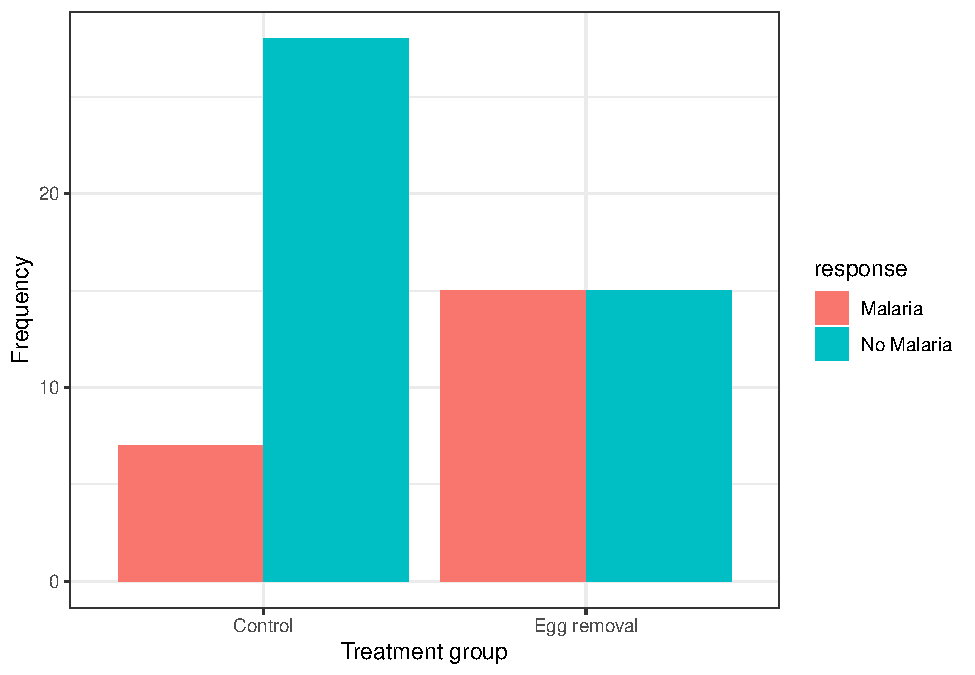
\includegraphics{BIOL202_files/figure-latex/malaria_barchart1-1.pdf}

This code is similar to what we used \hyperref[vis_cat_barchart]{previously to create a bar graph}, but there are two key differences:

\begin{itemize}
\tightlist
\item
  in the first line within the \texttt{aes} function, we include a new argument \texttt{fill\ =\ response}, telling R to use different bar fill colours based on the categories in the ``response'' variable.\\
\item
  in the second line, we provide a new argument to the \texttt{geom\_bar} function: \texttt{position\ =\ position\_dodge()}, which tells R to use separate bars for each category of the ``fill'' variable (if we did not include this argument, we'd get a ``stacked bar graph'' instead)
\end{itemize}

It is best practice to use the \textbf{response variable} as the ``fill'' variable in a grouped bar graph, as we have done in the malaria example.

If we wished to provide an appropriate figure heading, this would be the code:

\begin{figure}
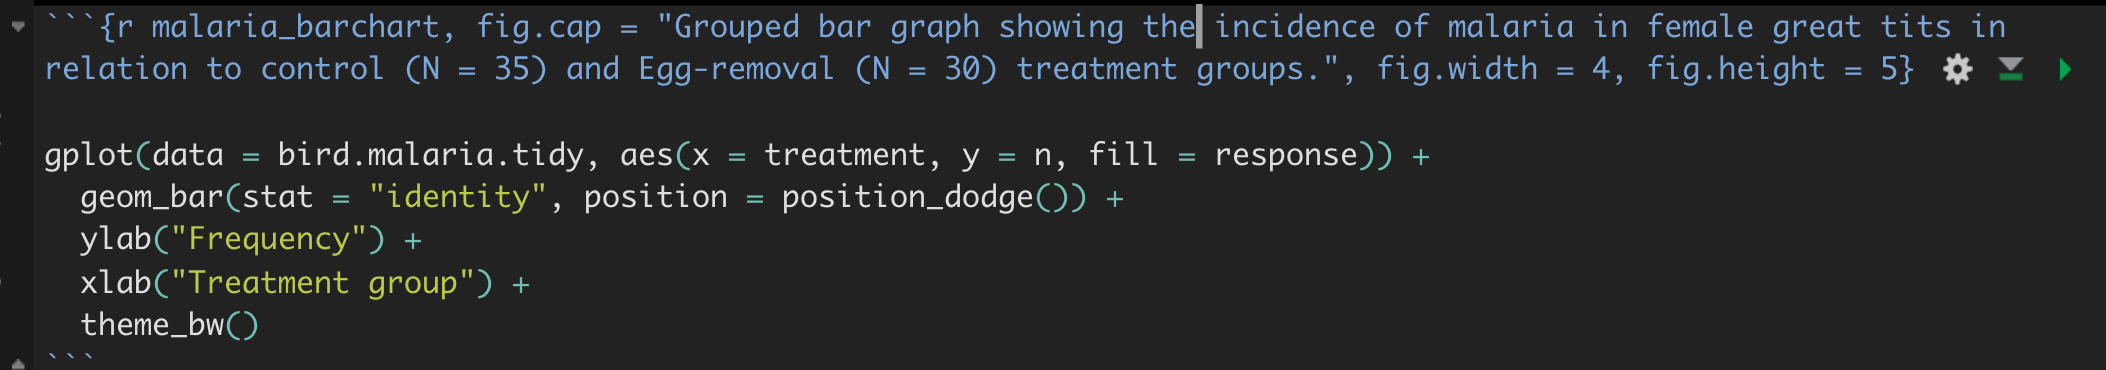
\includegraphics[width=29.25in]{./more/grouped_bar_graph} \caption{Example code chunk for producing a good grouped bar graph}\label{fig:unnamed-chunk-42}
\end{figure}

And the result:

\begin{Shaded}
\begin{Highlighting}[]
\FunctionTok{ggplot}\NormalTok{(}\AttributeTok{data =}\NormalTok{ bird.malaria.tidy, }\FunctionTok{aes}\NormalTok{(}\AttributeTok{x =}\NormalTok{ treatment, }\AttributeTok{y =}\NormalTok{ n, }\AttributeTok{fill =}\NormalTok{ response)) }\SpecialCharTok{+} 
  \FunctionTok{geom\_bar}\NormalTok{(}\AttributeTok{stat =} \StringTok{"identity"}\NormalTok{, }\AttributeTok{position =} \FunctionTok{position\_dodge}\NormalTok{()) }\SpecialCharTok{+} 
  \FunctionTok{ylab}\NormalTok{(}\StringTok{"Frequency"}\NormalTok{) }\SpecialCharTok{+}
  \FunctionTok{xlab}\NormalTok{(}\StringTok{"Treatment group"}\NormalTok{) }\SpecialCharTok{+}
  \FunctionTok{theme\_bw}\NormalTok{()}
\end{Highlighting}
\end{Shaded}

\begin{figure}
\centering
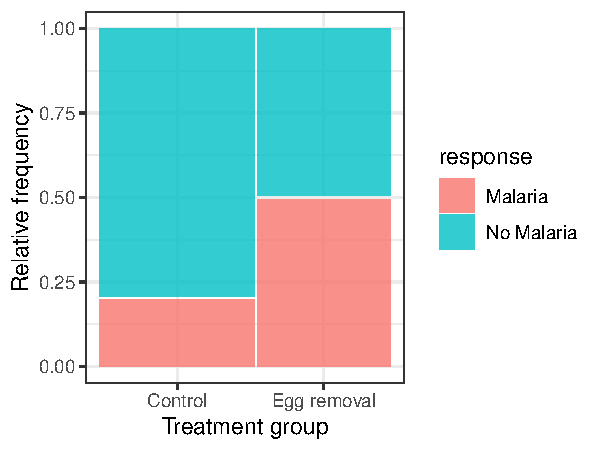
\includegraphics{BIOL202_files/figure-latex/unnamed-chunk-43-1.pdf}
\caption{\label{fig:unnamed-chunk-43}Grouped bar graph showing the incidence of malaria in female great tits in relation to control (N = 35) and Egg-removal (N = 30) treatment groups.}
\end{figure}

\subsection{Constructing a mosaic plot}\label{mosaic_plot}

An alternative and often more effective way to visualize the association between two categorical variables is a \textbf{mosaic plot}.

For this we use the \texttt{geom\_mosaic} function, from the \texttt{ggmosaic} package, in conjunction with the \texttt{ggplot} function.

For more information about the \texttt{ggmosaic} package, see this \href{https://cran.r-project.org/web/packages/ggmosaic/vignettes/ggmosaic.html}{vignette}.

For the \texttt{geom\_mosaic} function, we actually use the original (raw) \texttt{bird.malaria} tibble, which has a row for every observation (i.e.~it isn't summarized first into a frequency table).

Here's the code, and we'll explain after:

\begin{Shaded}
\begin{Highlighting}[]
\FunctionTok{ggplot}\NormalTok{(}\AttributeTok{data =}\NormalTok{ bird.malaria) }\SpecialCharTok{+}
  \FunctionTok{geom\_mosaic}\NormalTok{(}\FunctionTok{aes}\NormalTok{(}\AttributeTok{x =} \FunctionTok{product}\NormalTok{(treatment), }\AttributeTok{fill =}\NormalTok{ response)) }\SpecialCharTok{+}
  \FunctionTok{scale\_y\_continuous}\NormalTok{() }\SpecialCharTok{+}
  \FunctionTok{xlab}\NormalTok{(}\StringTok{"Treatment group"}\NormalTok{) }\SpecialCharTok{+}
  \FunctionTok{ylab}\NormalTok{(}\StringTok{"Relative frequency"}\NormalTok{) }\SpecialCharTok{+}
  \FunctionTok{theme\_bw}\NormalTok{()}
\end{Highlighting}
\end{Shaded}

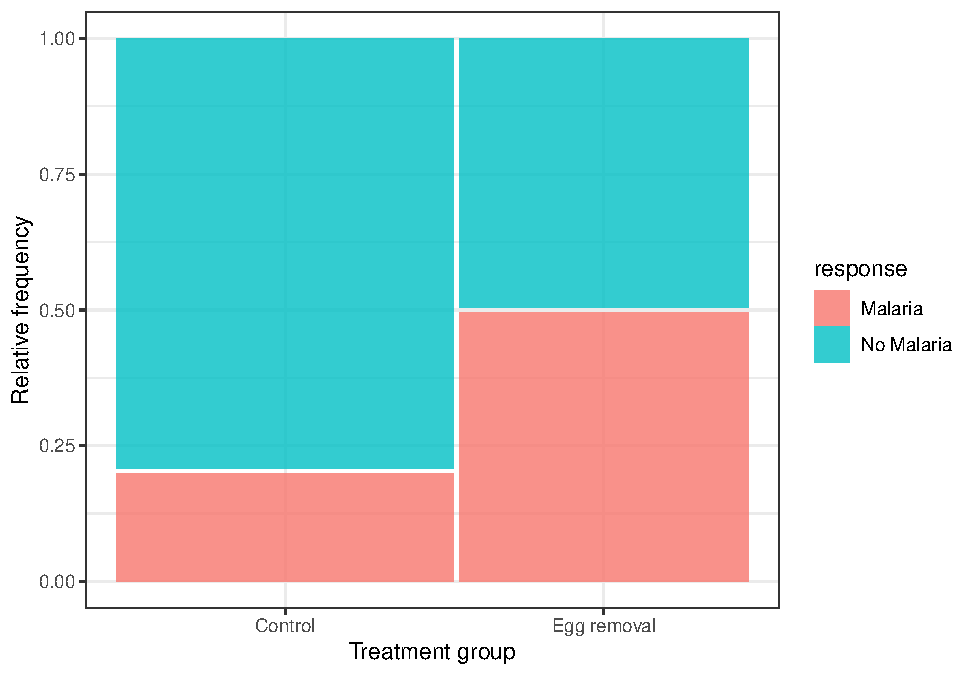
\includegraphics{BIOL202_files/figure-latex/mosaic_malaria1-1.pdf}

In the code chunk above we see one key difference from previous uses of the \texttt{ggplot} function is that the \texttt{aes} function is not provided in the arguments to \texttt{ggplot} in the first line, but is instead provided to the arguments of the \texttt{geom\_mosaic} function on the second line.

We also see \texttt{product(treatment)}, which is difficult to explain, so suffice it to say that it's telling the \texttt{geom\_mosaic} function to calculate relative frequencies based on the ``treatment'' variable, and in conjunction with the fill variable ``response''.

The \texttt{scale\_y\_continuous} function tells ggplot to add a continuous scale for the y-axis, and here, this defaults to zero to one for relative frequencies.

We'll learn about interpreting mosaic plots next.

\begin{enumerate}
\def\labelenumi{\arabic{enumi}.}
\tightlist
\item
  Using the \texttt{penguins} dataset, try creating a mosaic plot for comparing the relative frequency of penguins belonging to the three different ``species'' across the three different islands (variable ``island'').
\end{enumerate}

\subsection{Interpreting mosaic plots}\label{interpret_mosaic}

Let's provide the mosaic plot again, and this time we'll provide an appropriate figure heading in the chunk header, as we \hyperref[rmd_graphing]{learned previously}:

\begin{Shaded}
\begin{Highlighting}[]
\FunctionTok{ggplot}\NormalTok{(}\AttributeTok{data =}\NormalTok{ bird.malaria) }\SpecialCharTok{+}
  \FunctionTok{geom\_mosaic}\NormalTok{(}\FunctionTok{aes}\NormalTok{(}\AttributeTok{x =} \FunctionTok{product}\NormalTok{(treatment), }\AttributeTok{fill =}\NormalTok{ response)) }\SpecialCharTok{+}
  \FunctionTok{scale\_y\_continuous}\NormalTok{() }\SpecialCharTok{+}
  \FunctionTok{xlab}\NormalTok{(}\StringTok{"Treatment group"}\NormalTok{) }\SpecialCharTok{+}
  \FunctionTok{ylab}\NormalTok{(}\StringTok{"Relative frequency"}\NormalTok{) }\SpecialCharTok{+}
  \FunctionTok{theme\_bw}\NormalTok{()}
\end{Highlighting}
\end{Shaded}

\begin{figure}
\centering
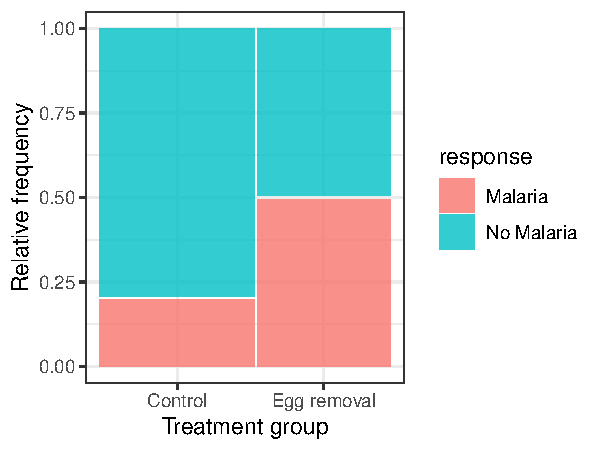
\includegraphics{BIOL202_files/figure-latex/unnamed-chunk-44-1.pdf}
\caption{\label{fig:unnamed-chunk-44}Relative frequency of the incidence of malaria in female great tits in relation to control (N = 35) and Egg-removal (N = 30) treatment groups.}
\end{figure}

Here's the code:

\begin{figure}
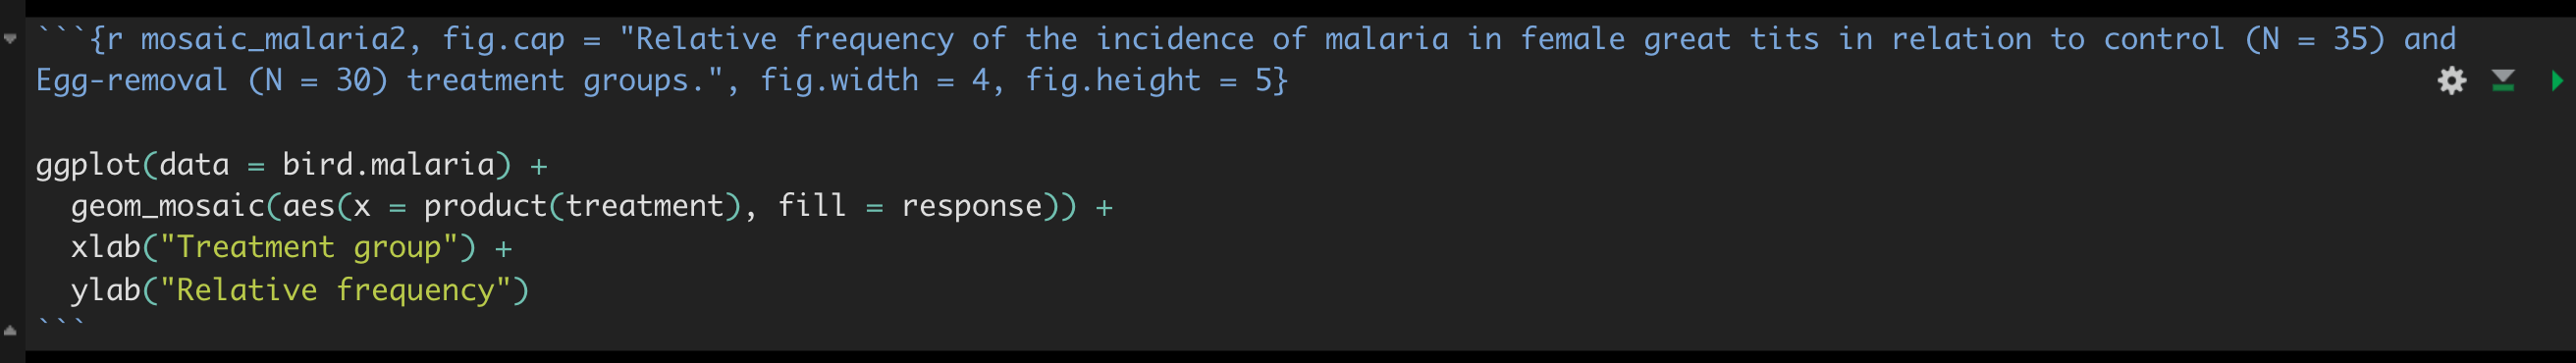
\includegraphics[width=29.56in]{./more/mosaic_graph} \caption{Example code chunk for producing a good mosaic plot}\label{fig:unnamed-chunk-45}
\end{figure}

When interpreting a mosaic plot, the key is to look how the relative frequency of the categories of the response variable - denoted by the ``fill'' colours - varies across the explanatory variable, which is arranged on the x-axis.

For example, in the malaria example above:

``The mosaic plot shows that the incidence (or relative frequency) of malaria is comparatively greater among birds in the egg removal treatment group compared to the control group. Only about 20\% of birds in the control group contracted malaria, whereas 50\% of the birds in the the egg-removal group contracted malaria.''

\section{Visualizing association between two numeric variables}\label{two_numeric}

We use a \textbf{scatterplot} to show association between two numerical variables.

We'll use the \texttt{ggplot} function that we've seen before, along with \texttt{geom\_point} to construct a scatterplot.

We'll provide an example using the \texttt{penguins} dataset, examining how bill depth and length are associated among the penguins belonging to the Adelie species.

As shown in the tutorial on \hyperref[rmd_graphing]{preparing and formatting assignments}, we can use the \texttt{filter} function from the \texttt{dplyr} package to easily subset datasets according to some criterion, such as belonging to a specific category.

\begin{Shaded}
\begin{Highlighting}[]
\NormalTok{penguins }\SpecialCharTok{\%\textgreater{}\%} 
  \FunctionTok{filter}\NormalTok{(species }\SpecialCharTok{==} \StringTok{"Adelie"}\NormalTok{) }\SpecialCharTok{\%\textgreater{}\%}
\FunctionTok{ggplot}\NormalTok{(}\FunctionTok{aes}\NormalTok{(}\AttributeTok{x =}\NormalTok{ bill\_length\_mm, }\AttributeTok{y =}\NormalTok{ bill\_depth\_mm)) }\SpecialCharTok{+}
  \FunctionTok{geom\_point}\NormalTok{(}\AttributeTok{shape =} \DecValTok{1}\NormalTok{) }\SpecialCharTok{+}
  \FunctionTok{xlab}\NormalTok{(}\StringTok{"Bill length (mm)"}\NormalTok{) }\SpecialCharTok{+}
  \FunctionTok{ylab}\NormalTok{(}\StringTok{"Bill depth (mm)"}\NormalTok{) }\SpecialCharTok{+}
  \FunctionTok{theme\_bw}\NormalTok{()}
\end{Highlighting}
\end{Shaded}

\begin{figure}
\centering
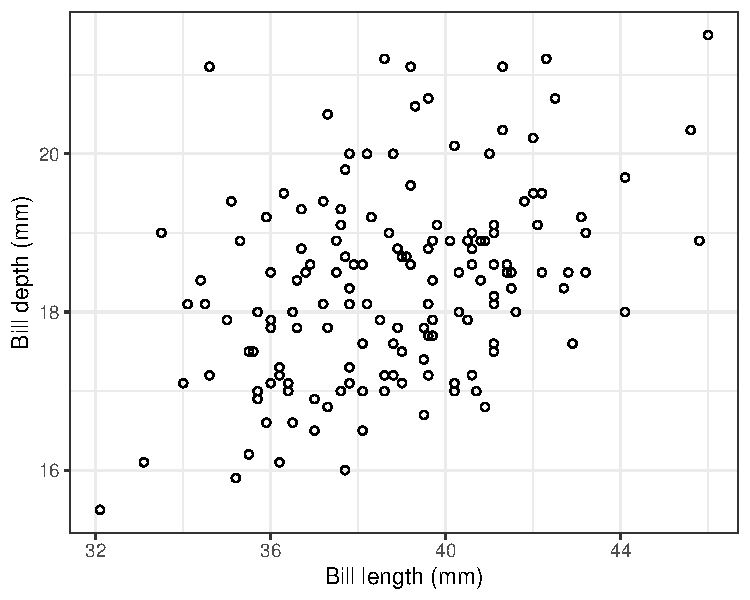
\includegraphics{BIOL202_files/figure-latex/unnamed-chunk-46-1.pdf}
\caption{\label{fig:unnamed-chunk-46}Scatterplot of the association between bill length and depth among 151 Adelie penguins}
\end{figure}

In the code chunk above, we have:

\begin{itemize}
\tightlist
\item
  the input tibble \texttt{penguins} followed by the pipe (``\%\textgreater\%'')
\item
  the \texttt{filter} function with the criterion used for subsetting, specifically any cases in which the ``species'' categorical variable equals ``Adelie''
\item
  then we provide the \texttt{ggplot} function and its \texttt{aes} argument, specifying the x- and y- variables to be used
\item
  then we use \texttt{geom\_point} to tell R to create a scatterplot using points, and specifically ``shape = 1'' denotes hollow circles
\item
  then we have x and y labels, followed by the \texttt{theme\_bw} function telling R to use black and white theme
\end{itemize}

Notice that the figure caption indicates the number of observations (sample size) used in the plot. In a \hyperref[vis_describe]{previous tutorial} it was emphasized that one needs to be careful in tallying the actual number of observations being used in a graph or when calculating descriptive statistics. For example, there is one missing value (``NA'') in the bill measurements for the Adelie penguins, hence the sample size of 151 instead of 152.

Recall that you can use the \texttt{skim} or \texttt{skim\_without\_charts} functions to get an overview of a dataset or of a single variable in a dataset, and to figure out how many missing values there are for each variable. You can also use the \texttt{summarise} function, as described \hyperref[mean_sd]{previously}.

\subsection{Interpreting and describing a scatterplot}\label{interpret_scatter}

Things to report when describing a scatterplot:

\begin{itemize}
\tightlist
\item
  is there an association? A ``shotgun blast'' pattern indicates no. If there is an association, is it \emph{positive} or \emph{negative}?
\item
  if there is an association, is it weak, moderate, or strong?
\item
  is the association \emph{linear}? If not, is there a different pattern like concave down?
\item
  are there any \emph{outlier} observations that lie far from the general trend?
\end{itemize}

In the scatterplot above, bill length and depth are positively associated, and the association is moderately strong. There are no observations that are strongly inconsistent with the general trend, though one individual with bill length of around 35mm and depth of around 21mm may be somewhat unusual.

\begin{enumerate}
\def\labelenumi{\arabic{enumi}.}
\tightlist
\item
  Using the \texttt{penguins} dataset, create a scatterplot of flipper length in relation to body mass, and provide an appropriate figure caption.
\end{enumerate}

\section{Visualizing association between a numeric and a categorical variable}\label{numeric_vs_cat}

To visualize association between a numerical response variable and a categorical explanatory variable, we have a variety of options, and the choice depends in part on the sample sizes within the categories being visualized.

\begin{itemize}
\tightlist
\item
  When sample sizes are relatively small in each category, such as 20 or fewer, use a \textbf{stripchart}
\item
  When sample sizes are larger (\textgreater20), use a \textbf{violin plot}, or less ideal, a \textbf{boxplot}.
\end{itemize}

We'll use locust serotonin data set from the text book. Consult figure 2.1-2 in the text for a description.

Always remember to get an overview of the dataset before attempting to create graphs, and not only for establishing sample sizes. If you had gotten an overview of the \texttt{locust} dataset, you would see we have a numeric response variable ``serotoninLevel'', but the categorical (explanatory) variable ``treatmentTime'' is actually coded as a numerical variable, with values of 0, 1, or 2 hours. Although this variable is coded as numeric, we can treat it as though it is an ordinal categorical variable.

We should re-code the ``treatmentTime'' variable in the \texttt{locust} dataset as a ``factor'' variable with three ``levels'': 0, 1, 2. This is not necessary for our graphs to work, but it is good practice to do this when you encounter this situation where a variable that should be treated as an ordinal categorical variable is coded as numerical.

We do this using the \texttt{as.factor} function, as follows:

\begin{Shaded}
\begin{Highlighting}[]
\NormalTok{locust}\SpecialCharTok{$}\NormalTok{treatmentTime }\OtherTok{\textless{}{-}} \FunctionTok{as.factor}\NormalTok{(locust}\SpecialCharTok{$}\NormalTok{treatmentTime)}
\end{Highlighting}
\end{Shaded}

Before creating a stripchart, it's a good idea to prepare a table of descriptive stats for your numerical response variable grouped by the categorical variable.

\begin{center}\rule{0.5\linewidth}{0.5pt}\end{center}

\begin{enumerate}
\def\labelenumi{\arabic{enumi}.}
\tightlist
\item
  Using what you learned in a \hyperref[desc_numeric_var_cat]{previous tutorial}, create a table of descriptive statistics of serotonin levels grouped by the treatment group variable.
\end{enumerate}

\begin{center}\rule{0.5\linewidth}{0.5pt}\end{center}

\subsection{Create a stripchart}\label{stripchart}

Now we're ready to create a stripchart of the locust experiment data. Note that we're not yet ready to add ``error bars'' to our strip chart; that will come in a later tutorial.

We'll provide the code, then explain after:

\begin{Shaded}
\begin{Highlighting}[]
\NormalTok{locust }\SpecialCharTok{\%\textgreater{}\%} 
  \FunctionTok{ggplot}\NormalTok{(}\FunctionTok{aes}\NormalTok{(}\AttributeTok{x =}\NormalTok{ treatmentTime, }\AttributeTok{y =}\NormalTok{ serotoninLevel)) }\SpecialCharTok{+}
  \FunctionTok{geom\_jitter}\NormalTok{(}\AttributeTok{colour =} \StringTok{"black"}\NormalTok{, }\AttributeTok{size =} \DecValTok{3}\NormalTok{, }\AttributeTok{shape =} \DecValTok{1}\NormalTok{, }\AttributeTok{width =} \FloatTok{0.1}\NormalTok{) }\SpecialCharTok{+}
  \FunctionTok{xlab}\NormalTok{(}\StringTok{"Treatment time (hours)"}\NormalTok{) }\SpecialCharTok{+}
  \FunctionTok{ylab}\NormalTok{(}\StringTok{"Serotonin (pmoles)"}\NormalTok{) }\SpecialCharTok{+}
  \FunctionTok{ylim}\NormalTok{(}\DecValTok{0}\NormalTok{, }\DecValTok{25}\NormalTok{) }\SpecialCharTok{+}
  \FunctionTok{theme\_bw}\NormalTok{()}
\end{Highlighting}
\end{Shaded}

\begin{figure}
\centering
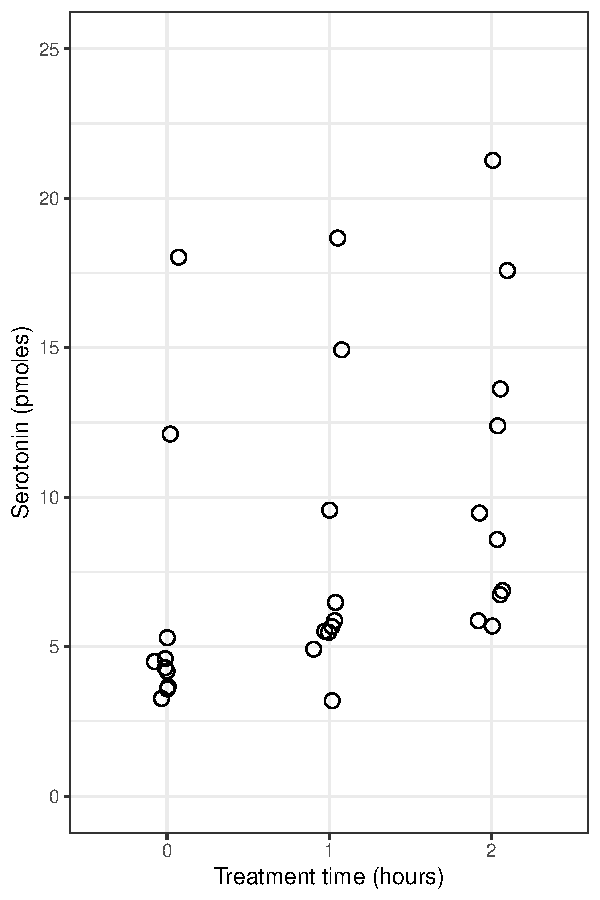
\includegraphics{BIOL202_files/figure-latex/unnamed-chunk-47-1.pdf}
\caption{\label{fig:unnamed-chunk-47}Serotonin levels in the central nervous system of desert locusts that were experimentally crowded for 0 (control), 1, and 2 hours. N = 10 per treatment group.}
\end{figure}

\begin{itemize}
\tightlist
\item
  the \texttt{ggplot} line of code is familiar
\item
  the new function here is the \texttt{geom\_jitter} function that simply plots the points in each group such that they are ``jittered'' or offset from one-another (to make them more visible). Its arguments include `colour = ``black''\,' telling R to use black points, ``size = 3'' to make the points a little larger than the default (1), ``shape = 1'' denoting hollow circles, and ``width = 0.1'' telling R to jitter the points a relatively small amount in the horizontal direction. Feel free to play with this arguments to get a feel for how they work.
\item
  the x- and y-axis labels come next
\item
  then we specify the minimum and maximum limits to the y-axis using the \texttt{ylim} function
\end{itemize}

Notice how all the data are visible! And it's evident that in the control and 1-hour treatment groups the majority of locusts exhibited comparatively low levels of serotonin (note the clusters of points).

\subsection{Create a violin plot}\label{violinplot}

Given that violin plots are best suited to when one has larger sample sizes per group, we'll go back to the \texttt{penguins} dataset for this, and evaluate how body mass of male penguins varies among species.

Let's first find out more about the data for the male penguins, so that we can include sample sizes in our figure captions. Specifically, we'll tally the number of complete body mass observations for each species, and also the number of missing values (NAs).

We'll combine the \texttt{filter} function with the \texttt{group\_by} function that we learned about in a \hyperref[desc_numeric_var_cat]{previous tutorial}:

\begin{Shaded}
\begin{Highlighting}[]
\NormalTok{penguins }\SpecialCharTok{\%\textgreater{}\%}
  \FunctionTok{filter}\NormalTok{(sex }\SpecialCharTok{==} \StringTok{"male"}\NormalTok{) }\SpecialCharTok{\%\textgreater{}\%}
  \FunctionTok{group\_by}\NormalTok{(species) }\SpecialCharTok{\%\textgreater{}\%}
  \FunctionTok{summarise}\NormalTok{(}
    \AttributeTok{Count =} \FunctionTok{n}\NormalTok{() }\SpecialCharTok{{-}}\NormalTok{ naniar}\SpecialCharTok{::}\FunctionTok{n\_miss}\NormalTok{(body\_mass\_g),}
    \AttributeTok{Count\_NA =}\NormalTok{ naniar}\SpecialCharTok{::}\FunctionTok{n\_miss}\NormalTok{(body\_mass\_g))}
\end{Highlighting}
\end{Shaded}

\begin{verbatim}
## # A tibble: 3 x 3
##   species   Count Count_NA
##   <fct>     <int>    <int>
## 1 Adelie       73        0
## 2 Chinstrap    34        0
## 3 Gentoo       61        0
\end{verbatim}

This is the same code we used \hyperref[desc_numeric_var_cat]{previously} for calculating descriptive statistics using a grouping variable (though we've eliminated some of the descriptive statistics here), but we inserted the \texttt{filter} function in the second line to make sure we're only using the male penguin records.

We now have the accurate sample sizes for each species (under the ``Count'' variable) we need to report in any figure caption.

We use the familiar \texttt{ggplot} approach for creating violin plots.

When using the \texttt{ggplot} function, we can assign the output to an object. We can then subsequently add features to the plot by adding to the object. We'll demonstrate this here.

Let's assign the basic violin plot to an object called ``bodymass.violin'', and we'll explain the rest of the code after:

\begin{Shaded}
\begin{Highlighting}[]
\NormalTok{bodymass.violin }\OtherTok{\textless{}{-}}\NormalTok{ penguins }\SpecialCharTok{\%\textgreater{}\%} 
  \FunctionTok{filter}\NormalTok{(sex }\SpecialCharTok{==} \StringTok{"male"}\NormalTok{) }\SpecialCharTok{\%\textgreater{}\%}
  \FunctionTok{ggplot}\NormalTok{(}\FunctionTok{aes}\NormalTok{(}\AttributeTok{x =}\NormalTok{ species, }\AttributeTok{y =}\NormalTok{ body\_mass\_g)) }\SpecialCharTok{+}
  \FunctionTok{geom\_violin}\NormalTok{() }\SpecialCharTok{+}
  \FunctionTok{xlab}\NormalTok{(}\StringTok{"Species"}\NormalTok{) }\SpecialCharTok{+}
  \FunctionTok{ylab}\NormalTok{(}\StringTok{"Body mass (g)"}\NormalTok{) }\SpecialCharTok{+}
  \FunctionTok{theme\_bw}\NormalTok{()}
\end{Highlighting}
\end{Shaded}

\begin{itemize}
\tightlist
\item
  We assign the output to the object called ``bodymass.violin'', and tell R which data object we're using (penguins)
\item
  We then \texttt{filter} the dataset to include only male penguins (sex == ``male''), and note the two equal signs and the quotations around ``male''
\item
  Then the familar \texttt{ggplot} with its \texttt{aes} argument
\item
  Now the new \texttt{geom\_violin} function, and it has optional arguments that we haven't used (see help file for the function)
\item
  Then the familiar labels and theme functions
\end{itemize}

Let's now have a look at the graph, and to do so, we simply type the name of the graph object we created:

\begin{Shaded}
\begin{Highlighting}[]
\NormalTok{bodymass.violin}
\end{Highlighting}
\end{Shaded}

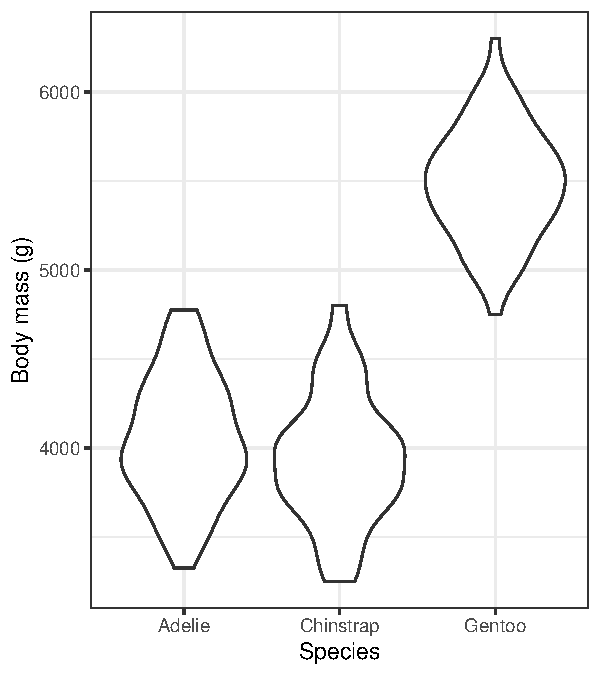
\includegraphics{BIOL202_files/figure-latex/body_violin-1.pdf}

One problem with the above graph is that we don't see the individual data points.

We can add those using the \texttt{geom\_jitter} function we learned about when \hyperref[stripchart]{creating stripcharts}.

Here's how we add features to an existing \texttt{ggplot} graph object, and we can again create a new object, or simply replace the old one.

Here, we'll create a new object called ``bodymass.violin.points'':

\begin{Shaded}
\begin{Highlighting}[]
\NormalTok{bodymass.violin.points }\OtherTok{\textless{}{-}}\NormalTok{ bodymass.violin }\SpecialCharTok{+} \FunctionTok{geom\_jitter}\NormalTok{(}\AttributeTok{size =} \DecValTok{2}\NormalTok{, }\AttributeTok{shape =} \DecValTok{1}\NormalTok{, }\AttributeTok{width =} \FloatTok{0.1}\NormalTok{)}
\end{Highlighting}
\end{Shaded}

And now show the plot:

\begin{Shaded}
\begin{Highlighting}[]
\NormalTok{bodymass.violin.points}
\end{Highlighting}
\end{Shaded}

\begin{figure}
\centering
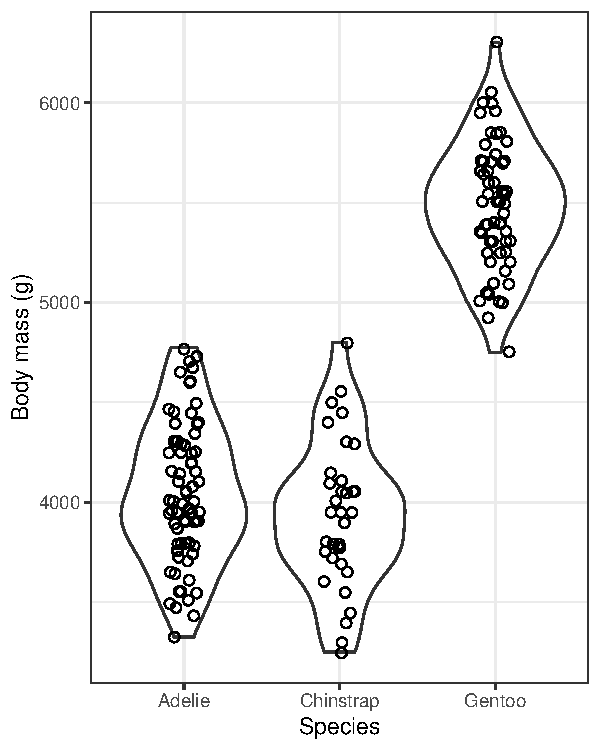
\includegraphics{BIOL202_files/figure-latex/unnamed-chunk-48-1.pdf}
\caption{\label{fig:unnamed-chunk-48}Violin plot showing the body mass (g) of male Adelie (N = 73), Chinstrap (N = 34), and Gentoo (N = 61) penguins.}
\end{figure}

\textbf{TIP}: If you wish to run all the code at once in a single chunk to create a figure, rather than adding new code to an existing object, here's what you'd include in your chunk (but here we don't show the chunk header that would include the caption):

\begin{verbatim}
penguins %>% 
  filter(sex == "male") %>%
  ggplot(aes(x = species, y = body_mass_g)) +
  geom_violin() +
  geom_jitter(size = 2, shape = 1, width = 0.1) +
  xlab("Species") +
  ylab("Body mass (g)") +
  theme_bw()
\end{verbatim}

To help understand what the violin plot is showing, we'll provide a new \textbf{bonus} graph that adds something called ``density plots'' to the margin of the violin plot.

Don't worry about replicating this type of graph, but if you can, fantastic!

First we create the main \texttt{ggplot} violin plot object:

\begin{Shaded}
\begin{Highlighting}[]
\NormalTok{bodymass.violin2 }\OtherTok{\textless{}{-}}\NormalTok{ penguins }\SpecialCharTok{\%\textgreater{}\%} 
  \FunctionTok{filter}\NormalTok{(sex }\SpecialCharTok{==} \StringTok{"male"}\NormalTok{) }\SpecialCharTok{\%\textgreater{}\%}
  \FunctionTok{ggplot}\NormalTok{() }\SpecialCharTok{+}
  \FunctionTok{geom\_violin}\NormalTok{(}\FunctionTok{aes}\NormalTok{(}\AttributeTok{x =}\NormalTok{ species, }\AttributeTok{y =}\NormalTok{ body\_mass\_g, }\AttributeTok{colour =}\NormalTok{ species)) }\SpecialCharTok{+}
  \FunctionTok{geom\_jitter}\NormalTok{(}\FunctionTok{aes}\NormalTok{(}\AttributeTok{x =}\NormalTok{ species, }\AttributeTok{y =}\NormalTok{ body\_mass\_g, }\AttributeTok{colour =}\NormalTok{ species), }\AttributeTok{size =} \DecValTok{2}\NormalTok{, }\AttributeTok{shape =} \DecValTok{1}\NormalTok{, }\AttributeTok{width =} \FloatTok{0.1}\NormalTok{) }\SpecialCharTok{+}
  \FunctionTok{xlab}\NormalTok{(}\StringTok{"Species"}\NormalTok{) }\SpecialCharTok{+}
  \FunctionTok{ylab}\NormalTok{(}\StringTok{"Body mass (g)"}\NormalTok{) }\SpecialCharTok{+}
  \FunctionTok{ylim}\NormalTok{(}\DecValTok{3000}\NormalTok{, }\DecValTok{6300}\NormalTok{) }\SpecialCharTok{+}
  \FunctionTok{theme\_bw}\NormalTok{() }\SpecialCharTok{+}
  \FunctionTok{theme}\NormalTok{(}\AttributeTok{legend.position =} \StringTok{"bottom"}\NormalTok{) }\SpecialCharTok{+}
  \FunctionTok{guides}\NormalTok{(}\AttributeTok{colour =} \FunctionTok{guide\_legend}\NormalTok{(}\AttributeTok{title=}\StringTok{"Species"}\NormalTok{))}
\end{Highlighting}
\end{Shaded}

Now we add density plots in the margins using the \texttt{ggMarginal} function from the \texttt{ggExtra} package:

\begin{Shaded}
\begin{Highlighting}[]
\FunctionTok{ggMarginal}\NormalTok{(bodymass.violin2, }\AttributeTok{type =} \StringTok{"density"}\NormalTok{, }\AttributeTok{alpha =} \FloatTok{0.3}\NormalTok{, }\AttributeTok{groupFill =} \ConstantTok{TRUE}\NormalTok{)}
\end{Highlighting}
\end{Shaded}

\begin{figure}
\centering
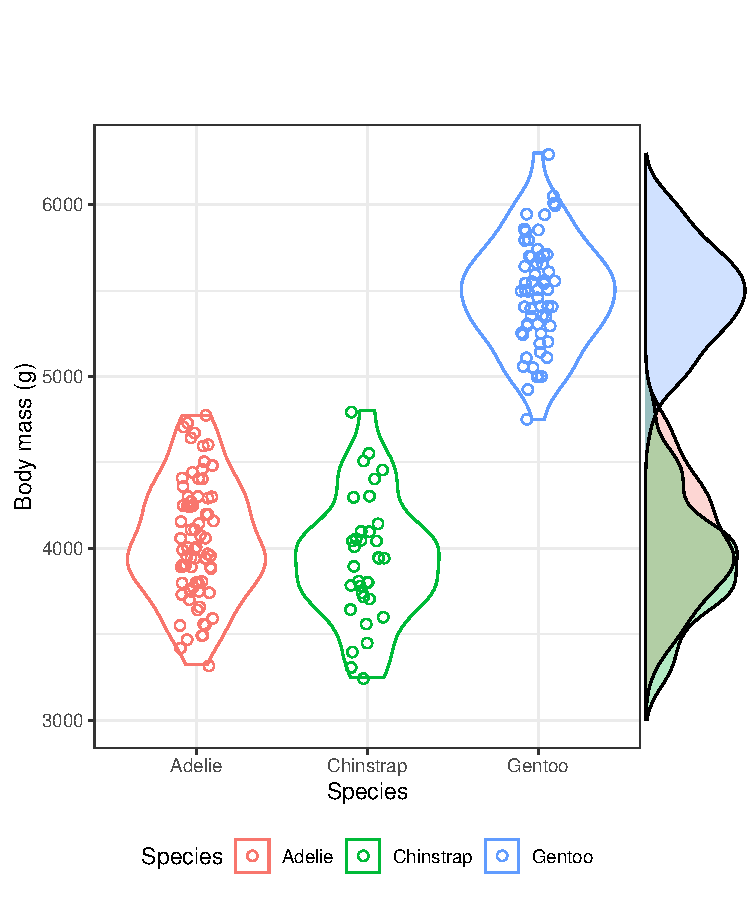
\includegraphics{BIOL202_files/figure-latex/unnamed-chunk-49-1.pdf}
\caption{\label{fig:unnamed-chunk-49}Violin plot showing the body mass (g) of male Adelie (N = 73), Chinstrap (N = 34), and Gentoo (N = 61) penguins. Density plots are provided in the margin.}
\end{figure}

The violin plot is designed to give an idea of the frequency distribution of response variable values within each group. Specifically, the width of the violin reflects the frequency of observations in that range of values. This is evident in the above figure within the ``density plots'' that are provided in the right-hand margin. Consider these density plots as a smoothed out version of a histogram.

We can see, for example, that for all three species of penguin there is a bulge in the middle indicating that there is a central mode to the body mass values in each group, with fewer values towards lower and higher extremes. The frequency distribution for the Gentoo species approximates a ``bell shape'' distribution, for example (the blue data).

\subsection{Creating a boxplot}\label{boxplots}

Here we'll learn how to create basic boxplots, and also superimpose boxplots onto violin plots.

In future tutorials we'll learn how to add features to these types of graphs in order to complement statistical comparisons of a numerical response variable among categories (groups) of a categorical explanatory variable.

Here is the code for creating boxplots, again using the penguins body mass data, and this time the \texttt{geom\_boxplot} function:

\begin{Shaded}
\begin{Highlighting}[]
\NormalTok{penguins }\SpecialCharTok{\%\textgreater{}\%} 
  \FunctionTok{filter}\NormalTok{(sex }\SpecialCharTok{==} \StringTok{"male"}\NormalTok{) }\SpecialCharTok{\%\textgreater{}\%}
  \FunctionTok{ggplot}\NormalTok{(}\FunctionTok{aes}\NormalTok{(}\AttributeTok{x =}\NormalTok{ species, }\AttributeTok{y =}\NormalTok{ body\_mass\_g)) }\SpecialCharTok{+}
  \FunctionTok{geom\_boxplot}\NormalTok{() }\SpecialCharTok{+}
  \FunctionTok{xlab}\NormalTok{(}\StringTok{"Species"}\NormalTok{) }\SpecialCharTok{+}
  \FunctionTok{ylab}\NormalTok{(}\StringTok{"Body mass (g)"}\NormalTok{) }\SpecialCharTok{+}
  \FunctionTok{theme\_bw}\NormalTok{()}
\end{Highlighting}
\end{Shaded}

\begin{figure}
\centering
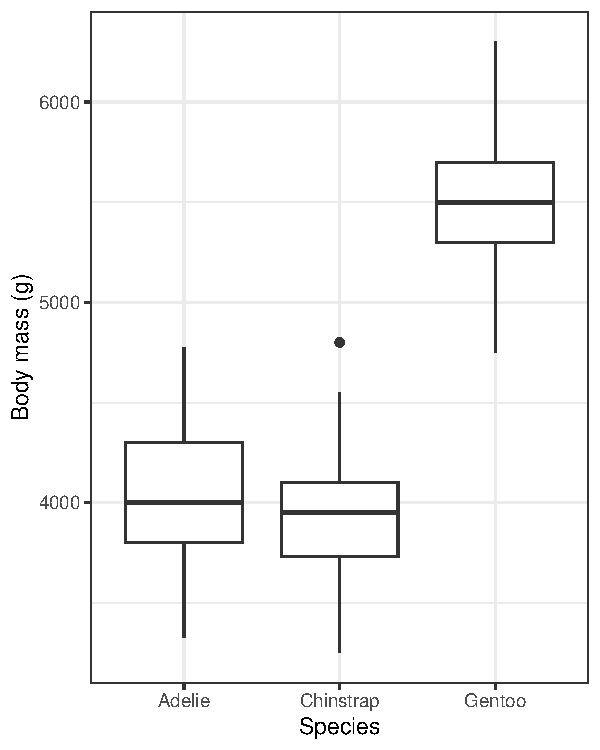
\includegraphics{BIOL202_files/figure-latex/unnamed-chunk-50-1.pdf}
\caption{\label{fig:unnamed-chunk-50}Boxplot showing the body mass (g) of male Adelie (N = 73), Chinstrap (N = 34), and Gentoo (N = 61) penguins. Density plots are provided in the margin. Boxes delimit the first and third quartiles, and the middle line depicts the median. Whiskers extend to values beyond the 1st (lower) and 3rd (upper) quartiles, up to a maximum of 1.5 x IQR, and individual black points are outlying values.}
\end{figure}

For more information about the features of the boxplot, look at the help file for the \texttt{geom\_boxplot} function:

\begin{verbatim}
?geom_boxplot
\end{verbatim}

The first time you include a boxplot in a report / lab, be sure to include in the figure caption the details of what is being shown. You only need to do this the first time. Subsequent boxplot figure captions can refer to the first one for details.

When sample sizes are large in each group, like they are for the penguins data we've been visualizing, the most ideal way to visualize the data is to combine violin and boxplots. We'll do this next!

\subsection{Combining violin and boxplots}\label{bestplot}

Superimposing boxplots onto violin plots (and of course, showing individual points too!) provides for a very informative graph.

We already have a basic violin plot object created, called ``bodymass.violin'', so let's start with that, then add the boxplot information, then superimpose the points. We need to do it in that order, so that the points become the ``top'' layer of information, and aren't hidden behind the boxplot or violins.

\begin{Shaded}
\begin{Highlighting}[]
\NormalTok{bodymass.violin }\SpecialCharTok{+} 
  \FunctionTok{geom\_boxplot}\NormalTok{(}\AttributeTok{width =} \FloatTok{0.1}\NormalTok{) }\SpecialCharTok{+} 
  \FunctionTok{geom\_jitter}\NormalTok{(}\AttributeTok{colour =} \StringTok{"grey"}\NormalTok{, }\AttributeTok{size =} \DecValTok{1}\NormalTok{, }\AttributeTok{shape =} \DecValTok{1}\NormalTok{, }\AttributeTok{width =} \FloatTok{0.15}\NormalTok{)}
\end{Highlighting}
\end{Shaded}

\begin{figure}
\centering
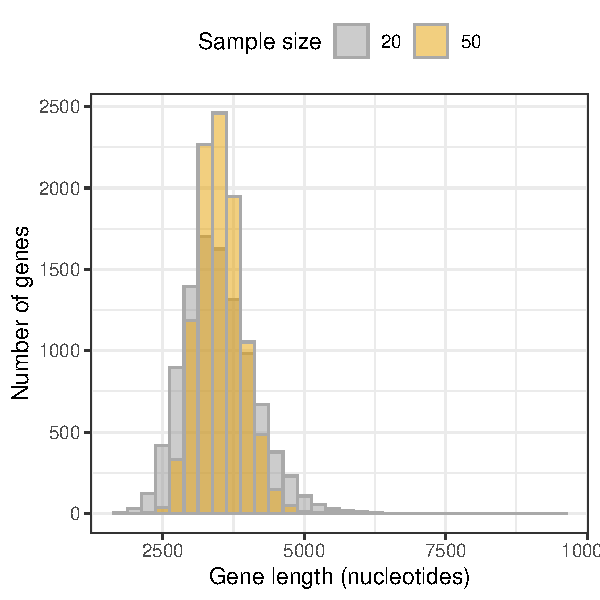
\includegraphics{BIOL202_files/figure-latex/unnamed-chunk-51-1.pdf}
\caption{\label{fig:unnamed-chunk-51}Violin plot showing the body mass (g) of male Adelie (N = 73), Chinstrap (N = 34), and Gentoo (N = 61) penguins. Boxplots are superimposed, with boxes delimiting the first and third quartiles, and middle line depicting the median. Whiskers extend to values beyond the 1st (lower) and 3rd (upper) quartiles, up to a maximum of 1.5 x IQR, and individual black points are outlying values.}
\end{figure}

\begin{itemize}
\tightlist
\item
  We start with the base violin plot object ``bodymass.violin''
\item
  We then add the boxplot using \texttt{geom\_boxplot}, ensuring that the boxes are narrow in width (width = 0.1) so they don't overwhelm the violins
\item
  We then add the individual data points using \texttt{geom\_jitter}, and this time using the colour ``grey'' so that they don't obscure the black boxes underneath, and making them a bit smaller this time (size = 1), and keeping them as hollow circles (shape = 1), and this time spreading them out horizontally a bit more (width = 0.15)
\end{itemize}

\textbf{TIP}: if you'd rather do all the code in one chunk, without creating objects, here's what you'd include:

\begin{verbatim}
penguins %>% 
  filter(sex == "male") %>%
  ggplot(aes(x = species, y = body_mass_g)) +
  geom_violin() +
  geom_boxplot(width = 0.1) + 
  geom_jitter(colour = "grey", size = 1, shape = 1, width = 0.15) +
  xlab("Species") +
  ylab("Body mass (g)") +
  theme_bw()
\end{verbatim}

It often takes some playing around with argument values before one gets the ideal graph. For example, in the above graph, try changing some of the values used in the \texttt{geom\_jitter} function.

\begin{enumerate}
\def\labelenumi{\arabic{enumi}.}
\tightlist
\item
  Using the \texttt{penguins} dataset, and only the records pertaining to female penguins, create a combined violin / boxplot graph showing bill length in relation to species. Include an appropriate figure caption.
\end{enumerate}

\subsection{Interpreting stripcharts, violin plots and boxplots}\label{interp_violin}

In general, stripcharts, violin plots, and boxplots are used to visualize how a numeric variable varies or differs among categories (groups) of a categorical variable. For instance, it's pretty obvious from the violin plots above that Gentoo penguins have, on average, considerably greater body mass than the other two species. We will wait until a future tutorial to learn more about interpreting violin / boxplots, because there we learn how to add more information to the graphs, such as group means and measures of uncertainty. For now, you should be comfortable interpreting any obvious patterns in the plots.

\part*{Inferential Statistics}\label{part-inferential-statistics}
\addcontentsline{toc}{part}{Inferential Statistics}

\chapter{Sampling, Estimation, \& Uncertainty}\label{estimation}

\textbf{Tutorial learning objectives}

In this tutorial you will:

\begin{itemize}
\tightlist
\item
  Learn how to take a random sample of observations from a dataset
\item
  Learn through simulation what ``sampling error'' is
\item
  Learn about sampling distributions through simulation
\item
  Learn how to calculate the standard error of the mean
\item
  Learn how to calculate the ``rule of thumb 95\% confidence interval''
\end{itemize}

\section{Load packages and import data}\label{estimation_packages_data}

Let's load some familiar packages first:

\begin{Shaded}
\begin{Highlighting}[]
\FunctionTok{library}\NormalTok{(tidyverse)}
\FunctionTok{library}\NormalTok{(naniar)}
\FunctionTok{library}\NormalTok{(knitr)}
\FunctionTok{library}\NormalTok{(skimr)}
\end{Highlighting}
\end{Shaded}

We will also need a new package called \texttt{infer}, so install that package using the procedure you \hyperref[package_install]{previously learned}, then load it:

\begin{Shaded}
\begin{Highlighting}[]
\FunctionTok{library}\NormalTok{(infer)}
\end{Highlighting}
\end{Shaded}

\textbf{Import Data}

For this tutorial we'll use the human gene length dataset that is used in Chapter 4 of the Whitlock \& Schluter text.

The dataset is described in example 4.1 in the text.

Let's import it:

\begin{Shaded}
\begin{Highlighting}[]
\NormalTok{genelengths }\OtherTok{\textless{}{-}} \FunctionTok{read\_csv}\NormalTok{(}\StringTok{"https://raw.githubusercontent.com/ubco{-}biology/BIOL202/main/data/humangenelength.csv"}\NormalTok{)}
\end{Highlighting}
\end{Shaded}

\begin{verbatim}
## Rows: 22385 Columns: 4
## -- Column specification --------------------------------------------------------
## Delimiter: ","
## chr (3): gene, name, description
## dbl (1): size
## 
## i Use `spec()` to retrieve the full column specification for this data.
## i Specify the column types or set `show_col_types = FALSE` to quiet this message.
\end{verbatim}

\textbf{Get an overview of the data}

We'll use \texttt{skim\_without\_charts} to get an overview:

\begin{Shaded}
\begin{Highlighting}[]
\NormalTok{genelengths }\SpecialCharTok{\%\textgreater{}\%}
  \FunctionTok{skim\_without\_charts}\NormalTok{()}
\end{Highlighting}
\end{Shaded}

(\#tab:est\_overview)Data summary

Name

Piped data

Number of rows

22385

Number of columns

4

\_\_\_\_\_\_\_\_\_\_\_\_\_\_\_\_\_\_\_\_\_\_\_

Column type frequency:

character

3

numeric

1

\_\_\_\_\_\_\_\_\_\_\_\_\_\_\_\_\_\_\_\_\_\_\_\_

Group variables

None

\textbf{Variable type: character}

skim\_variable

n\_missing

complete\_rate

min

max

empty

n\_unique

whitespace

gene

0

1.00

17

18

0

22385

0

name

0

1.00

2

15

0

19906

0

description

432

0.98

1

51

0

4183

0

\textbf{Variable type: numeric}

skim\_variable

n\_missing

complete\_rate

mean

sd

p0

p25

p50

p75

p100

size

0

1

3511.46

2833.29

69

1684

2744

4511

109224

The ``size'' variable is the key one: it includes the gene lengths (number of nucleotides) for each of the 22385 genes in the dataset.

\section{Functions for sampling}\label{sampling_functions}

To illustrate the concepts of ``sampling error'' and the ``sampling distribution of the mean'', we're going to make use of datasets that include measurements for all individuals in a ``population'' of interest, and we're going to take random samples of observations from those datasets. This mimics the process of sampling at random from a population.

There are two functions that are especially helpful for taking random samples from objects.

\begin{itemize}
\tightlist
\item
  The \texttt{sample} function in the base R package is easy to use for taking a random sample from a \textbf{vector} of values. Look at the help function for it:
\end{itemize}

\begin{verbatim}
?sample
\end{verbatim}

The second useful function is the \texttt{slice\_sample} function from the \texttt{dplyr} package (loaded with \texttt{tidyverse}). This function takes random samples of rows from a \textbf{dataframe} or \textbf{tibble}.

\begin{verbatim}
?slice_sample
\end{verbatim}

Note that both functions have a \texttt{replace} argument that dictates whether the sampling we conduct occurs with or without replacement. For instance, the following code will not work (try copying and pasting into your console):

\begin{verbatim}
sample(1:6, size = 10, replace = F)
\end{verbatim}

Here we're telling R to sample 10 values from a vector that includes only 6 values (one through six), and with the \texttt{replace\ =\ F} argument we told R not to put the sampled numbers back in the pile for future sampling.

If instead we specified \texttt{replace\ =\ T}, as shown below, then we be conducting \emph{sampling with replacement}, and sampled values are placed back in the pool each time, thus enabling the code to work (try it):

\begin{verbatim}
sample(1:6, size = 10, replace = T)
\end{verbatim}

Whether we wish to \emph{sample without replacement} or not depends on the question / context (see page 138 in Whitlock \& Schluter). For most of the questions and contexts we deal with in this course, we do wish to sample \textbf{with} replacement. Why? Because we are typically assuming (or mimicking a situation) that we're randomly sampling from a very large population, in which case the probability distribution of possible values in the individuals that remain doesn't change when we sample. This is not the case if we're sampling from a small population.

\subsection{Setting the ``seed'' for random sampling}\label{setseed}

Functions such as \texttt{sample} and \texttt{slice\_sample} have a challenge to meet: they must be able to take samples that are as as random as possible. On a computer, this is easier said then done; special algorithms are required to meet the challenge. R has some pretty good ones available, so we don't have to worry about it (though to be honest, they can only generate ``pseudorandom'' numbers, but that's good enough for our purposes!).

However, we DO need to worry about \emph{computational reproducibility}.

Imagine we have authored a script for a research project, and the script makes use of functions such as \texttt{sample}. Now imagine that someone else wanted to re-run our analyses on their own computer. Any code chunks that included functions such as \texttt{sample} would produce different results for them, because the function takes a different random sample each time it's run!

Thankfully there's a way to ensure that scripts implementing random sampling can be computationally reproducible: we can use the \texttt{set.seed} function.

This assumes you are using R version 4 or later (e.g.~4.1). The \texttt{set.seed} function used a different default algorithm in versions of R prior to version 4.0.

Let's provide the code chunk then explain after:

\begin{Shaded}
\begin{Highlighting}[]
\FunctionTok{set.seed}\NormalTok{(}\DecValTok{12}\NormalTok{)}
\end{Highlighting}
\end{Shaded}

The \texttt{set.seed} function requires an integer value as an argument. You can pick any number you want as the seed number. Here we'll use 12, and if you do too, you'll get the same results as in the tutorial.

Let's test this using the \texttt{runif} function, which generates random numbers between user-designated minimum and maximum values (the default is numbers between zero and one).

Let's include the \texttt{set.seed} function right before using the \texttt{runif} function, and here we'll again use a seed number of 12.

\begin{Shaded}
\begin{Highlighting}[]
\FunctionTok{set.seed}\NormalTok{(}\DecValTok{12}\NormalTok{)}
\FunctionTok{runif}\NormalTok{(}\DecValTok{3}\NormalTok{)}
\end{Highlighting}
\end{Shaded}

\begin{verbatim}
## [1] 0.06936092 0.81777520 0.94262173
\end{verbatim}

Here we told the \texttt{runif} function to generate three random numbers, and it used the default minimum and maximum values of zero and one.

Now let's try a different seed:

\begin{Shaded}
\begin{Highlighting}[]
\FunctionTok{set.seed}\NormalTok{(}\DecValTok{25}\NormalTok{)}
\FunctionTok{runif}\NormalTok{(}\DecValTok{3}\NormalTok{)}
\end{Highlighting}
\end{Shaded}

\begin{verbatim}
## [1] 0.4161184 0.6947637 0.1488006
\end{verbatim}

So long as you used the same seed number, you should have gotten the same three random numbers as shown above.

When you are authoring your own script or markdown document (e.g.~for a research project), it is advisable to only set the seed once, at the beginning of your script or markdown document. When you run or knit your completed script/markdown, the seed will be set at the beginning, the code chunks will run in sequence, and each chunk that uses a random number generator will do so in a predictable way (based on the seed number). The script will be computationally reproducible. In contrast, when we're trying out code (e.g.~when working on tutorial material), we aren't running a set sequence or number of code chunks, so we can't rely on everyone getting the same output for a particular code chunk. For this reason you'll see in the tutorial material that many of the code chunks that require use of a random number generator will include a \texttt{set.seed} statement, to ensure that everyone gets the same output from that specific code chunk (this isn't always required, but often it is).

\begin{enumerate}
\def\labelenumi{\arabic{enumi}.}
\tightlist
\item
  Generate 10 random numbers using the \texttt{runif} function, and first set the seed number to 200.
\end{enumerate}

\section{Sampling error}\label{sampling_error}

\begin{quote}
\textbf{Sampling error} is the chance difference, caused by sampling, between an estimate and the population parameter being estimated
\end{quote}

Here we'll get a feel for \textbf{sampling error} using the human gene data.

Let's use the \texttt{slice\_sample} function to randomly sample \emph{n} = 20 rows from the \texttt{genelengths} tibble, and store them in a tibble object called ``randsamp1'':

\begin{Shaded}
\begin{Highlighting}[]
\FunctionTok{set.seed}\NormalTok{(}\DecValTok{12}\NormalTok{)}
\NormalTok{randsamp1 }\OtherTok{\textless{}{-}}\NormalTok{ genelengths }\SpecialCharTok{\%\textgreater{}\%}
  \FunctionTok{slice\_sample}\NormalTok{(}\AttributeTok{n =} \DecValTok{20}\NormalTok{, }\AttributeTok{replace =} \ConstantTok{FALSE}\NormalTok{) }\SpecialCharTok{\%\textgreater{}\%}
  \FunctionTok{select}\NormalTok{(size)}
\end{Highlighting}
\end{Shaded}

In the preceding chunk, we:

\begin{itemize}
\tightlist
\item
  set the seed (here using integer 12), so that everyone gets the same output for this code chunk
\item
  tell R that we want the output from our code to be stored in an object named ``randsamp1''
\item
  use the \texttt{slice\_sample} function to randomly sample 20 rows from the \texttt{genelengths} tibble, and to do so without replacement
\item
  use the \texttt{select} function to tell R to return only the ``size'' variable from the newly generated (sampled) tibble
\end{itemize}

Now let's use the \texttt{mean} and \texttt{sd} base functions to calculate the mean and standard deviation using our sample.

We'll assign the calculations to an object ``randsamp1.mean.sd'', then we'll present the output using the \texttt{kable} function.

\begin{Shaded}
\begin{Highlighting}[]
\NormalTok{randsamp1.mean.sd }\OtherTok{\textless{}{-}}\NormalTok{ randsamp1 }\SpecialCharTok{\%\textgreater{}\%}
  \FunctionTok{summarise}\NormalTok{(}
    \AttributeTok{Mean\_genelength =} \FunctionTok{mean}\NormalTok{(size, }\AttributeTok{na.rm =} \ConstantTok{TRUE}\NormalTok{),}
    \AttributeTok{SD\_genelength =} \FunctionTok{sd}\NormalTok{(size, }\AttributeTok{na.rm =} \ConstantTok{TRUE}\NormalTok{)}
\NormalTok{  )}
\end{Highlighting}
\end{Shaded}

Now present the output using the \texttt{kable} function so we can control the maximum number of digits shown.

Using the \texttt{kable} approach to presenting tibble outputs ensures that, when knitted, your output shows a sufficient number of decimal places\ldots{} something that doesn't always happen without using the \texttt{kable} function.

\begin{Shaded}
\begin{Highlighting}[]
\FunctionTok{kable}\NormalTok{(randsamp1.mean.sd, }\AttributeTok{digits =} \DecValTok{4}\NormalTok{)}
\end{Highlighting}
\end{Shaded}

Mean\_genelength

SD\_genelength

3408.25

1443.698

Do your numbers match those above?

Let's now draw another random sample of the same size (20), making sure to give the resulting tibble object a different name (``randsamp2''). Here, we won't set the seed again, because all that is required is for everyone to get a different sample from the first one above; we don't need to have everyone get the \emph{same} sample, but it's ok if we do.

\begin{Shaded}
\begin{Highlighting}[]
\NormalTok{randsamp2 }\OtherTok{\textless{}{-}}\NormalTok{ genelengths }\SpecialCharTok{\%\textgreater{}\%}
  \FunctionTok{slice\_sample}\NormalTok{(}\AttributeTok{n =} \DecValTok{20}\NormalTok{, }\AttributeTok{replace =} \ConstantTok{FALSE}\NormalTok{) }\SpecialCharTok{\%\textgreater{}\%}
  \FunctionTok{select}\NormalTok{(size)}
\end{Highlighting}
\end{Shaded}

And calculate the mean and sd:

\begin{Shaded}
\begin{Highlighting}[]
\NormalTok{randsamp2.mean.sd }\OtherTok{\textless{}{-}}\NormalTok{ randsamp2 }\SpecialCharTok{\%\textgreater{}\%}
  \FunctionTok{summarise}\NormalTok{(}
    \AttributeTok{Mean\_genelength =} \FunctionTok{mean}\NormalTok{(size, }\AttributeTok{na.rm =} \ConstantTok{TRUE}\NormalTok{),}
    \AttributeTok{SD\_genelength =} \FunctionTok{sd}\NormalTok{(size, }\AttributeTok{na.rm =} \ConstantTok{TRUE}\NormalTok{)}
\NormalTok{  )}
\end{Highlighting}
\end{Shaded}

And show using the \texttt{kable} function:

\begin{Shaded}
\begin{Highlighting}[]
\FunctionTok{kable}\NormalTok{(randsamp2.mean.sd, }\AttributeTok{digits =} \DecValTok{4}\NormalTok{)}
\end{Highlighting}
\end{Shaded}

Mean\_genelength

SD\_genelength

4381.35

2081.471

Are they the same as we saw using the first random sample? NO! This reflects \textbf{sampling error}.

\begin{enumerate}
\def\labelenumi{\arabic{enumi}.}
\tightlist
\item
  Repeat the process above to get a third sample of size 20 genes, and calculate the mean and standard deviation of gene length for that sample.
\end{enumerate}

\section{Sampling distribution of the mean}\label{sampdistmean}

Now let's learn code to conduct our own resampling exercise.

Let's repeat the sampling exercise we did in the preceding section concerning \hyperref[sampling_error]{sampling error}, but this time repeat it many times, say 10000 times.

We'll also calculate the mean gene length for each sample that we take, and store this value.

For this, we'll use the newly installed \texttt{infer} package, and its handy function \texttt{rep\_slice\_sample}, which complements the \texttt{slice\_sample} function we've used before.

Let's look at the code then explain after:

\begin{Shaded}
\begin{Highlighting}[]
\NormalTok{gene.means.n20 }\OtherTok{\textless{}{-}}\NormalTok{ genelengths }\SpecialCharTok{\%\textgreater{}\%}
  \FunctionTok{rep\_slice\_sample}\NormalTok{(}\AttributeTok{n =} \DecValTok{20}\NormalTok{, }\AttributeTok{replace =} \ConstantTok{FALSE}\NormalTok{, }\AttributeTok{reps =} \DecValTok{10000}\NormalTok{) }\SpecialCharTok{\%\textgreater{}\%}
  \FunctionTok{summarise}\NormalTok{(}
    \AttributeTok{mean\_length =} \FunctionTok{mean}\NormalTok{(size, }\AttributeTok{na.rm =}\NormalTok{ T),}
    \AttributeTok{sampsize =} \FunctionTok{as.factor}\NormalTok{(}\DecValTok{20}\NormalTok{)}
\NormalTok{  )}
\end{Highlighting}
\end{Shaded}

In the above chunk, we:

\begin{itemize}
\tightlist
\item
  Tell R to put the output from our functions into a new tibble object called ``gene.means.n20'', with the ``n20'' on the end denoting the fact that we used a sample size of 20 for these samples
\item
  use the \texttt{rep\_slice\_sample} function to sample n = 20 rows at random from the \texttt{genelengths} tibble, and repeat this ``reps = 10000'' times
\item
  next we use the familiar \texttt{summarise} function to then create a new variable ``mean\_length'', which in the next line we define as the mean of the values in the ``size'' variable (and recall, at this point we have a sample of 20 of these)
\item
  we also create a new categorical (factor) variable ``sampsize'' that indicates what sample size we used for this exercise, and we store it as a factor rather than a number (we're doing this because it will come in handy later)
\end{itemize}

Let's look at the first handful of rows in the newly created tibble:

\begin{Shaded}
\begin{Highlighting}[]
\NormalTok{gene.means.n20}
\end{Highlighting}
\end{Shaded}

\begin{verbatim}
## # A tibble: 10,000 x 3
##    replicate mean_length sampsize
##        <int>       <dbl> <fct>   
##  1         1       3094. 20      
##  2         2       4705. 20      
##  3         3       2576. 20      
##  4         4       2957. 20      
##  5         5       3060. 20      
##  6         6       3768. 20      
##  7         7       3412. 20      
##  8         8       4258. 20      
##  9         9       3242. 20      
## 10        10       3134. 20      
## # i 9,990 more rows
\end{verbatim}

We see that it is a tibble with 10000 rows and three columns: a variable called ``replicate'', which holds the numbers one through the number of replicates run (here, 10000), a variable ``mean\_length'' that we created, which holds the sample mean gene length for each of the replicate samples we took, and a variable ``sampsize'' that tells us the sample size used for each sample (here, 20).

\textbf{Pause:}
If we were to plot a histogram of these 10000 sample means, what shape do you think it would have? And what value do you think it would be centred on?

\subsection{Visualize the sampling distribution}\label{hist_samdist}

Let's plot a histogram of the 10000 means that we calculated.

First, to figure out what axis limits we should set for our histogram, let's get an idea of what the mean gene length values look like:

\begin{Shaded}
\begin{Highlighting}[]
\NormalTok{gene.means.n20 }\SpecialCharTok{\%\textgreater{}\%}
 \FunctionTok{skim\_without\_charts}\NormalTok{(mean\_length)}
\end{Highlighting}
\end{Shaded}

(\#tab:view\_means)Data summary

Name

Piped data

Number of rows

10000

Number of columns

3

\_\_\_\_\_\_\_\_\_\_\_\_\_\_\_\_\_\_\_\_\_\_\_

Column type frequency:

numeric

1

\_\_\_\_\_\_\_\_\_\_\_\_\_\_\_\_\_\_\_\_\_\_\_\_

Group variables

None

\textbf{Variable type: numeric}

skim\_variable

n\_missing

complete\_rate

mean

sd

p0

p25

p50

p75

p100

mean\_length

0

1

3497.63

621.56

1650.2

3066.16

3439.65

3871.6

9609.4

OK, so we see that the minimum and maximum values are 1650.2 (under the ``p0'' heading) and 9609.4 (under the ``p100'' heading). So this can inform our x-axis limits when constructing the histogram (note that you typically need to try out different maximum values for the y-axis limits).

Let's first remind ourselves what the true mean gene length is in the entire population of genes. We'll assign the output to an object ``true.mean.length'' and a variable called ``Pop\_mean'', then show using the \texttt{kable} approach.

\begin{Shaded}
\begin{Highlighting}[]
\NormalTok{true.mean.length }\OtherTok{\textless{}{-}}\NormalTok{ genelengths }\SpecialCharTok{\%\textgreater{}\%}
  \FunctionTok{summarise}\NormalTok{(}
    \AttributeTok{Pop\_mean =} \FunctionTok{mean}\NormalTok{(size, }\AttributeTok{na.rm =} \ConstantTok{TRUE}\NormalTok{)}
\NormalTok{  )}
\end{Highlighting}
\end{Shaded}

Show using \texttt{kable}:

\begin{Shaded}
\begin{Highlighting}[]
\FunctionTok{kable}\NormalTok{(true.mean.length, }\AttributeTok{digits =} \DecValTok{4}\NormalTok{)}
\end{Highlighting}
\end{Shaded}

Pop\_mean

3511.457

Now let's plot the histogram of 10000 sample means:

\begin{Shaded}
\begin{Highlighting}[]
\NormalTok{gene.means.n20 }\SpecialCharTok{\%\textgreater{}\%}
\FunctionTok{ggplot}\NormalTok{(}\FunctionTok{aes}\NormalTok{(}\AttributeTok{x =}\NormalTok{ mean\_length)) }\SpecialCharTok{+}
  \FunctionTok{geom\_histogram}\NormalTok{(}\AttributeTok{binwidth =} \DecValTok{250}\NormalTok{, }\AttributeTok{color =} \StringTok{"black"}\NormalTok{, }\AttributeTok{fill =} \StringTok{"lightgrey"}\NormalTok{) }\SpecialCharTok{+}
  \FunctionTok{ylim}\NormalTok{(}\DecValTok{0}\NormalTok{, }\DecValTok{1700}\NormalTok{) }\SpecialCharTok{+}
  \FunctionTok{xlim}\NormalTok{(}\DecValTok{1500}\NormalTok{, }\DecValTok{10000}\NormalTok{) }\SpecialCharTok{+}
  \FunctionTok{xlab}\NormalTok{(}\StringTok{"Gene length (nucleotides)"}\NormalTok{) }\SpecialCharTok{+}
  \FunctionTok{ylab}\NormalTok{(}\StringTok{"Number of genes"}\NormalTok{) }\SpecialCharTok{+}
  \FunctionTok{theme\_bw}\NormalTok{()}
\end{Highlighting}
\end{Shaded}

\begin{figure}
\centering
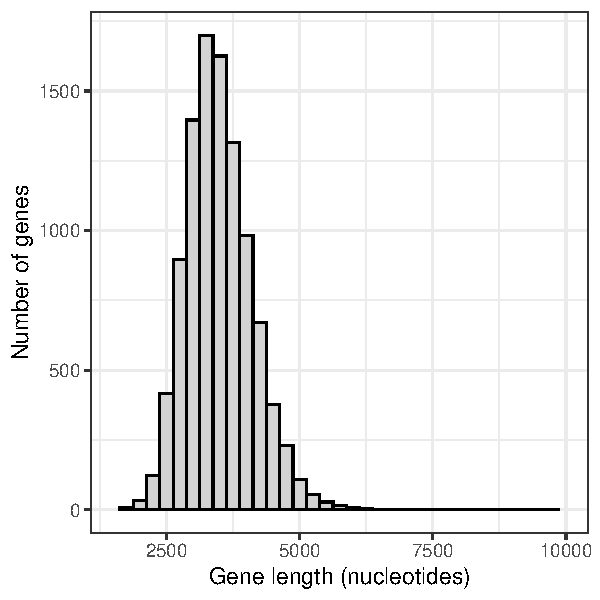
\includegraphics{BIOL202_files/figure-latex/unnamed-chunk-54-1.pdf}
\caption{\label{fig:unnamed-chunk-54}Approximate sampling distribution of mean gene lengths from the human genome (10000 replicate samples of size 20).}
\end{figure}

This histogram is an approximation of the \textbf{sampling distribution of the mean} for a sample size of 20 (to construct a real sampling distribution we'd need to take an infinite number of replicate samples).

Before interpreting the histogram, let's first calculate the mean of the 10000 sample means, then display using the \texttt{kable} approach:

\begin{Shaded}
\begin{Highlighting}[]
\NormalTok{sample.mean.n20 }\OtherTok{\textless{}{-}}\NormalTok{ gene.means.n20 }\SpecialCharTok{\%\textgreater{}\%}
  \FunctionTok{summarise}\NormalTok{(}
    \AttributeTok{Sample\_mean =} \FunctionTok{mean}\NormalTok{(mean\_length, }\AttributeTok{na.rm =} \ConstantTok{TRUE}\NormalTok{)}
\NormalTok{  )}
\end{Highlighting}
\end{Shaded}

Show using \texttt{kable}:

\begin{Shaded}
\begin{Highlighting}[]
\FunctionTok{kable}\NormalTok{(sample.mean.n20, }\AttributeTok{digits =} \DecValTok{4}\NormalTok{)}
\end{Highlighting}
\end{Shaded}

Sample\_mean

3497.633

Note that the mean of the sample means is around 3498, which is pretty darn close to the true population mean of 3511.

This reflects the fact that, provided a good random sample, the sample mean is an \textbf{unbiased estimate} of the true population mean.

Now, let's interpret the histogram:

\begin{itemize}
\tightlist
\item
  The vast majority of means are centred around the true population mean (around 3500)
\item
  The frequency distribution unimodal, but is right (positively) skewed; it has a handful of sample means that are very large
\end{itemize}

The latter characteristic reflects the fact that the population of genes includes more than 100 genes that are extremely large. When we take a random sample of 20 genes, it is possible that - just by chance - our sample could include one or more of the extremely large genes in the population, and this would of course inflate the magnitude of our mean gene length in the sample.

Let's repeat this sampling exersize using a larger sample size, say 50.

\begin{Shaded}
\begin{Highlighting}[]
\NormalTok{gene.means.n50 }\OtherTok{\textless{}{-}}\NormalTok{ genelengths }\SpecialCharTok{\%\textgreater{}\%}
  \FunctionTok{rep\_slice\_sample}\NormalTok{(}\AttributeTok{n =} \DecValTok{50}\NormalTok{, }\AttributeTok{replace =} \ConstantTok{FALSE}\NormalTok{, }\AttributeTok{reps =} \DecValTok{10000}\NormalTok{) }\SpecialCharTok{\%\textgreater{}\%}
  \FunctionTok{summarise}\NormalTok{(}
    \AttributeTok{mean\_length =} \FunctionTok{mean}\NormalTok{(size, }\AttributeTok{na.rm =}\NormalTok{ T),}
    \AttributeTok{sampsize =} \FunctionTok{as.factor}\NormalTok{(}\DecValTok{50}\NormalTok{)}
\NormalTok{  )}
\end{Highlighting}
\end{Shaded}

Now plot a histogram, making sure to keep the x- and y-axis limits the same as we used above, so that we can compare the outputs

\begin{Shaded}
\begin{Highlighting}[]
\NormalTok{gene.means.n50 }\SpecialCharTok{\%\textgreater{}\%}
\FunctionTok{ggplot}\NormalTok{(}\FunctionTok{aes}\NormalTok{(}\AttributeTok{x =}\NormalTok{ mean\_length)) }\SpecialCharTok{+}
  \FunctionTok{geom\_histogram}\NormalTok{(}\AttributeTok{binwidth =} \DecValTok{250}\NormalTok{, }\AttributeTok{color =} \StringTok{"black"}\NormalTok{, }\AttributeTok{fill =} \StringTok{"lightgrey"}\NormalTok{) }\SpecialCharTok{+}
  \FunctionTok{xlim}\NormalTok{(}\DecValTok{1500}\NormalTok{, }\DecValTok{10000}\NormalTok{) }\SpecialCharTok{+}
  \FunctionTok{xlab}\NormalTok{(}\StringTok{"Gene length (nucleotides)"}\NormalTok{) }\SpecialCharTok{+}
  \FunctionTok{ylab}\NormalTok{(}\StringTok{"Number of genes"}\NormalTok{) }\SpecialCharTok{+}
  \FunctionTok{theme\_bw}\NormalTok{()}
\end{Highlighting}
\end{Shaded}

\begin{figure}
\centering
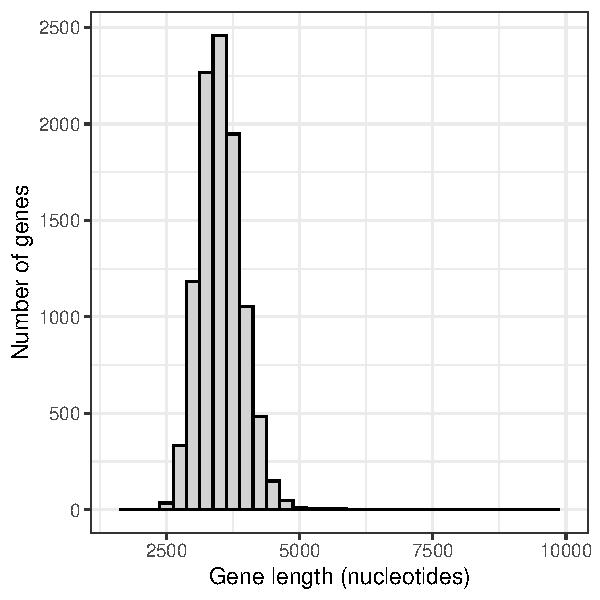
\includegraphics{BIOL202_files/figure-latex/unnamed-chunk-56-1.pdf}
\caption{\label{fig:unnamed-chunk-56}Approximate sampling distribution of mean gene lengths from the human genome (10000 replicate samples of size 50).}
\end{figure}

Notice that there is much less positive skew to this frequency distribution.

Let's produce a figure that allows us to directly compare the two sampling distributions.

First we need to combine the data into one tibble.

\textbf{New tool}
We can merge two tibbles (or data frames) together by rows using the \texttt{bind\_rows} function from the \texttt{dplyr} package

The \texttt{bind\_rows} function will simply append one object to another by rows. This requires that the two (or more) objects each have the same variables. In our case, the two objects have the same three variables.

\begin{Shaded}
\begin{Highlighting}[]
\NormalTok{gene.means.combined }\OtherTok{\textless{}{-}} \FunctionTok{bind\_rows}\NormalTok{(gene.means.n20, gene.means.n50)}
\end{Highlighting}
\end{Shaded}

Now we have what we need to produce a graph that enables direct comparison of the two sampling distributions.

This type of graph is not something you'll need to be able to do for assignments!

\begin{Shaded}
\begin{Highlighting}[]
\NormalTok{gene.means.combined }\SpecialCharTok{\%\textgreater{}\%}
 \FunctionTok{ggplot}\NormalTok{(}\FunctionTok{aes}\NormalTok{(}\AttributeTok{x =}\NormalTok{ mean\_length, }\AttributeTok{fill =} \FunctionTok{as.factor}\NormalTok{(sampsize))) }\SpecialCharTok{+}
  \FunctionTok{geom\_histogram}\NormalTok{(}\AttributeTok{position =} \StringTok{\textquotesingle{}identity\textquotesingle{}}\NormalTok{, }\AttributeTok{colour =} \StringTok{"darkgrey"}\NormalTok{, }\AttributeTok{alpha =} \FloatTok{0.5}\NormalTok{, }\AttributeTok{binwidth =} \DecValTok{250}\NormalTok{) }\SpecialCharTok{+}
  \FunctionTok{scale\_fill\_manual}\NormalTok{(}\AttributeTok{values=}\FunctionTok{c}\NormalTok{(}\StringTok{"\#999999"}\NormalTok{, }\StringTok{"\#E69F00"}\NormalTok{)) }\SpecialCharTok{+}
  \FunctionTok{xlab}\NormalTok{(}\StringTok{"Gene length (nucleotides)"}\NormalTok{) }\SpecialCharTok{+}
  \FunctionTok{ylab}\NormalTok{(}\StringTok{"Number of genes"}\NormalTok{) }\SpecialCharTok{+}
  \FunctionTok{theme\_bw}\NormalTok{() }\SpecialCharTok{+}
  \FunctionTok{theme}\NormalTok{(}\AttributeTok{legend.position =} \StringTok{"top"}\NormalTok{) }\SpecialCharTok{+}
  \FunctionTok{guides}\NormalTok{(}\AttributeTok{fill =} \FunctionTok{guide\_legend}\NormalTok{(}\AttributeTok{title =} \StringTok{"Sample size"}\NormalTok{))}
\end{Highlighting}
\end{Shaded}

\begin{figure}
\centering
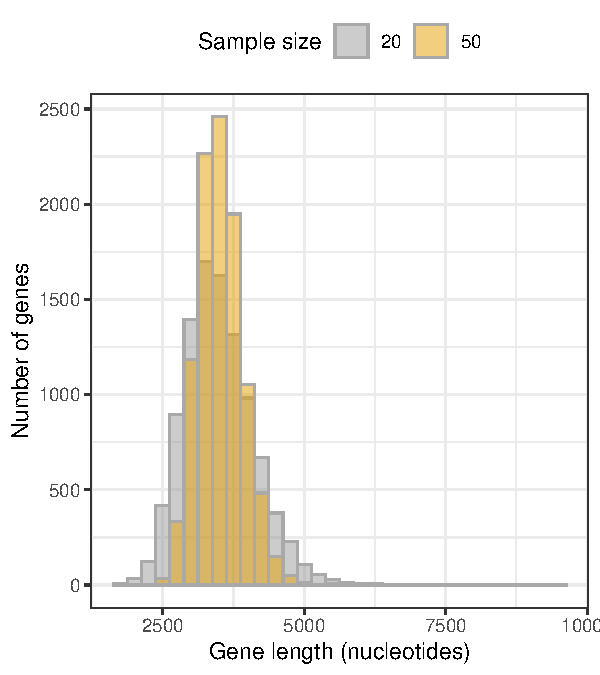
\includegraphics{BIOL202_files/figure-latex/newsampfig-1.pdf}
\caption{\label{fig:newsampfig}Approximate sampling distributions of mean gene lengths from the human genome, fig.height=, message=FALSE, warning=FALSE, using sample sizes of 20 and 50 (10000 replicate samples in each distribution).}
\end{figure}

We can see that the smaller sample size (20) yields a broader sampling distribution, and though it's a difficult to see, it also exhibits a longer tail towards larger gene lengths.

With larger sample sizes, we'll get more precise estimates of the true population mean!

\begin{enumerate}
\def\labelenumi{\arabic{enumi}.}
\tightlist
\item
  Follow this \href{http://www.zoology.ubc.ca/~whitlock/Kingfisher/SamplingNormal.htm}{online tutorial} that helps visualize the construction of a sampling distribution of the mean
\end{enumerate}

\section{Standard error of the mean}\label{sem_page}

This is the formula for calculating the \textbf{standard error} \textbf{of the mean} when the population parameter is unknown (which is usually the case):

\[SE_\bar{Y} = \frac{s}{\sqrt{n}}\]

This is one measure of uncertainty that we report alongside our sample-based estimate of the population mean.

It represents the standard deviation of the sampling distribution of the mean. Thus, it is a measure of spread for the sampling distribution of the mean.

\textbf{Calculating the SEM in R}

To illustrate how to calculate the SEM, we'll make use of the gene length dataset again.

Let's take a random sample of 20 genes, making sure to set the seed this time so everyone gets the same result. We'll use a seed number of 29, and we'll save our sample of values from the variable ``size'' in an object (tibble) called ``newsamp.n20'':

\begin{Shaded}
\begin{Highlighting}[]
\FunctionTok{set.seed}\NormalTok{(}\DecValTok{29}\NormalTok{)}
\NormalTok{newsamp.n20 }\OtherTok{\textless{}{-}}\NormalTok{ genelengths }\SpecialCharTok{\%\textgreater{}\%}
  \FunctionTok{slice\_sample}\NormalTok{(}\AttributeTok{n =} \DecValTok{20}\NormalTok{, }\AttributeTok{replace =} \ConstantTok{FALSE}\NormalTok{) }\SpecialCharTok{\%\textgreater{}\%}
  \FunctionTok{select}\NormalTok{(size)}
\end{Highlighting}
\end{Shaded}

Now let's show the code for calculating the SEM for the mean calculated using values in the ``size'' variable from our ``newsamp.n20'' object. We'll output stats to a new object ``newsamp.n20.stats'' then display the object using \texttt{kable}.

\begin{Shaded}
\begin{Highlighting}[]
\NormalTok{newsamp.n20.stats }\OtherTok{\textless{}{-}}\NormalTok{ newsamp.n20 }\SpecialCharTok{\%\textgreater{}\%}
  \FunctionTok{summarise}\NormalTok{(}
    \AttributeTok{Count =} \FunctionTok{n}\NormalTok{() }\SpecialCharTok{{-}}\NormalTok{ naniar}\SpecialCharTok{::}\FunctionTok{n\_miss}\NormalTok{(size),}
    \AttributeTok{Mean\_genelength =} \FunctionTok{mean}\NormalTok{(size, }\AttributeTok{na.rm =} \ConstantTok{TRUE}\NormalTok{),}
    \AttributeTok{SD\_genelength =} \FunctionTok{sd}\NormalTok{(size, }\AttributeTok{na.rm =} \ConstantTok{TRUE}\NormalTok{),}
    \AttributeTok{SEM =}\NormalTok{ SD\_genelength}\SpecialCharTok{/}\FunctionTok{sqrt}\NormalTok{(Count)}
\NormalTok{  )}
\end{Highlighting}
\end{Shaded}

You've seen all but the last lines of code before! Importantly, as we've seen \hyperref[mean_sd]{before}, the ``Count'' variable, calculatedusing the \texttt{n} function in combinatin with the \texttt{n\_miss} function from the \texttt{naniar} package, tallies the number of non-missing observations in the variable of interest (here, ``size''). This is the sample size that we'll need for the calculation of the SEM.

The last line creates a new variable ``SEM'' that is calculated using the formula shown above, and inputs from the previous lines' calculations.

Specifically, the sample size ``n'' value comes from the ``Count'' variable, and the ``s'' value comes from the ``SD\_genelength'' variable. And lastly, we use the \texttt{sqrt} function to take the square-root of the sample size.

Display the output:

\begin{Shaded}
\begin{Highlighting}[]
\FunctionTok{kable}\NormalTok{(newsamp.n20.stats, }\AttributeTok{digits =} \DecValTok{4}\NormalTok{)}
\end{Highlighting}
\end{Shaded}

Count

Mean\_genelength

SD\_genelength

SEM

20

3563.7

3747.552

837.9782

If you wish to calculate and report only the mean and SEM for a variable (here, the ``size'' variable from our tibble ``newsamp.n20''):

\begin{Shaded}
\begin{Highlighting}[]
\NormalTok{newsamp.n20.stats.short }\OtherTok{\textless{}{-}}\NormalTok{ newsamp.n20 }\SpecialCharTok{\%\textgreater{}\%}
  \FunctionTok{summarise}\NormalTok{(}
    \AttributeTok{Mean\_genelength =} \FunctionTok{mean}\NormalTok{(size, }\AttributeTok{na.rm =} \ConstantTok{TRUE}\NormalTok{),}
    \AttributeTok{SEM =} \FunctionTok{sd}\NormalTok{(size, }\AttributeTok{na.rm =} \ConstantTok{TRUE}\NormalTok{)}\SpecialCharTok{/}\FunctionTok{sqrt}\NormalTok{(}\FunctionTok{n}\NormalTok{() }\SpecialCharTok{{-}}\NormalTok{ naniar}\SpecialCharTok{::}\FunctionTok{n\_miss}\NormalTok{(size))}
\NormalTok{  )}
\end{Highlighting}
\end{Shaded}

Display the output:

\begin{Shaded}
\begin{Highlighting}[]
\FunctionTok{kable}\NormalTok{(newsamp.n20.stats.short, }\AttributeTok{digits =} \DecValTok{4}\NormalTok{)}
\end{Highlighting}
\end{Shaded}

Mean\_genelength

SEM

3563.7

837.9782

\textbf{TIP}
It is a good idea to use the longer approach that reports the sample size (``Count''), mean, standard deviation, and SEM. Why? Because in this way you're reporting each value (\emph{n} and \emph{s}) that goes into the calculation of the SEM.

\section{Rule of thumb 95\% confidence interval}\label{confint_rough}

The \textbf{Rule of Thumb} 95\% confidence interval is calculated simply as the sample mean +/- two standard errors.

Thus, the \textbf{lower confidence limit} is calculated as the sample mean minus 2 times the standard error, and the \textbf{upper confidence limit} is calculated as the sample mean plus 2 times the standard error.

We can re-use code from the previous section for the calculations, and we'll assign the output to a new object called ``newsamp.n20.allstats'':

\begin{Shaded}
\begin{Highlighting}[]
\NormalTok{newsamp.n20.allstats }\OtherTok{\textless{}{-}}\NormalTok{ newsamp.n20 }\SpecialCharTok{\%\textgreater{}\%}
  \FunctionTok{summarise}\NormalTok{(}
    \AttributeTok{Count =} \FunctionTok{n}\NormalTok{() }\SpecialCharTok{{-}}\NormalTok{ naniar}\SpecialCharTok{::}\FunctionTok{n\_miss}\NormalTok{(size),}
    \AttributeTok{Mean\_genelength =} \FunctionTok{mean}\NormalTok{(size, }\AttributeTok{na.rm =} \ConstantTok{TRUE}\NormalTok{),}
    \AttributeTok{SD\_genelength =} \FunctionTok{sd}\NormalTok{(size, }\AttributeTok{na.rm =} \ConstantTok{TRUE}\NormalTok{),}
    \AttributeTok{SEM =}\NormalTok{ SD\_genelength}\SpecialCharTok{/}\FunctionTok{sqrt}\NormalTok{(Count),}
    \AttributeTok{Lower\_95\_CL =}\NormalTok{ Mean\_genelength }\SpecialCharTok{{-}} \DecValTok{2} \SpecialCharTok{*}\NormalTok{ SEM,}
    \AttributeTok{Upper\_95\_CL =}\NormalTok{ Mean\_genelength }\SpecialCharTok{+} \DecValTok{2} \SpecialCharTok{*}\NormalTok{ SEM}
\NormalTok{  )}
\end{Highlighting}
\end{Shaded}

We've added two lines of code, one for the lower confidence limit and one for the upper confidence limit.

Notice that we again use calculations completed in preceding lines as input for the subsequent lines. Specifically, we use the ``Mean\_genelength'' value and the ``SEM'' value in our confidence limit calculations.

The asterisk (*) denotes multiplication.

Let's look at the output:

\begin{Shaded}
\begin{Highlighting}[]
\FunctionTok{kable}\NormalTok{(newsamp.n20.allstats, }\AttributeTok{digits =} \DecValTok{4}\NormalTok{)}
\end{Highlighting}
\end{Shaded}

Count

Mean\_genelength

SD\_genelength

SEM

Lower\_95\_CL

Upper\_95\_CL

20

3563.7

3747.552

837.9782

1887.744

5239.656

If you are asked to report the rule-of-thumb 95\% confidence \textbf{interval}, then you'd use the output from your calculations above to report:\\
\textbf{1887.744 \textless{} \(\mu\) \textless{} 5239.656}\\
Note that it is the population parameter being estimated, \(\mu\), that appears in between the lower and upper limits.

To produce greek letters such as ``mu'', simply precede the ``mu'' with a backslash, then enclose the entire term with dollar signs, as shown at this \href{http://www.evanlray.com/stat242_f2019/resources/R/MathinRmd.html}{webpage}.

\textbf{NOTE}: In a later tutorial you'll learn how to calculate actual confidence intervals, rather than ``rule of thumb'' confidence intervals

\chapter{Hypothesis testing}\label{hypothesis}

\textbf{Tutorial learning objectives}

\begin{itemize}
\tightlist
\item
  Learn the steps to conducting a hypothesis test
\item
  Learn how to simulate a null distribution (using a binomial distribution example)
\item
  Learn how to calculate the \emph{P}-value
\item
  Learn how write concluding statements for hypothesis tests
\end{itemize}

\section{Load packages and import data}\label{hyp_packages_data}

Load the \texttt{tidyverse}, \texttt{skimr}, \texttt{naniar}, and \texttt{infer} packages:

\begin{Shaded}
\begin{Highlighting}[]
\FunctionTok{library}\NormalTok{(tidyverse)}
\FunctionTok{library}\NormalTok{(skimr)}
\FunctionTok{library}\NormalTok{(infer)}
\FunctionTok{library}\NormalTok{(naniar)}
\end{Highlighting}
\end{Shaded}

Import the CSV file called ``damselfly'':

\begin{Shaded}
\begin{Highlighting}[]
\NormalTok{damselfly }\OtherTok{\textless{}{-}} \FunctionTok{read\_csv}\NormalTok{(}\StringTok{"https://raw.githubusercontent.com/ubco{-}biology/BIOL202/main/data/damselfly.csv"}\NormalTok{)}
\end{Highlighting}
\end{Shaded}

\begin{verbatim}
## Rows: 20 Columns: 1
## -- Column specification --------------------------------------------------------
## Delimiter: ","
## chr (1): direction
## 
## i Use `spec()` to retrieve the full column specification for this data.
## i Specify the column types or set `show_col_types = FALSE` to quiet this message.
\end{verbatim}

Get an overview of the dataset:

\begin{Shaded}
\begin{Highlighting}[]
\NormalTok{damselfly }\SpecialCharTok{\%\textgreater{}\%}
  \FunctionTok{skim\_without\_charts}\NormalTok{()}
\end{Highlighting}
\end{Shaded}

(\#tab:hyp\_overview)Data summary

Name

Piped data

Number of rows

20

Number of columns

1

\_\_\_\_\_\_\_\_\_\_\_\_\_\_\_\_\_\_\_\_\_\_\_

Column type frequency:

character

1

\_\_\_\_\_\_\_\_\_\_\_\_\_\_\_\_\_\_\_\_\_\_\_\_

Group variables

None

\textbf{Variable type: character}

skim\_variable

n\_missing

complete\_rate

min

max

empty

n\_unique

whitespace

direction

0

1

9

17

0

2

0

And view the first handful of rows:

\begin{Shaded}
\begin{Highlighting}[]
\NormalTok{damselfly}
\end{Highlighting}
\end{Shaded}

\begin{verbatim}
## # A tibble: 20 x 1
##    direction        
##    <chr>            
##  1 clockwise        
##  2 counter_clockwise
##  3 counter_clockwise
##  4 clockwise        
##  5 counter_clockwise
##  6 counter_clockwise
##  7 counter_clockwise
##  8 counter_clockwise
##  9 counter_clockwise
## 10 counter_clockwise
## 11 counter_clockwise
## 12 clockwise        
## 13 counter_clockwise
## 14 counter_clockwise
## 15 counter_clockwise
## 16 counter_clockwise
## 17 counter_clockwise
## 18 counter_clockwise
## 19 counter_clockwise
## 20 counter_clockwise
\end{verbatim}

\section{Steps to hypothesis testing}\label{hyp_steps}

Below is a list of all the steps required when conducting a hypothesis test.

Several of the steps we will learn about in later tutorials.

\begin{itemize}
\tightlist
\item
  Identify the appropriate statistical test and thus \textbf{null distribution} for the test statistic
\item
  State the null (\textbf{H\textsubscript{0}}) and alternative (\textbf{H\textsubscript{A}}) hypotheses\\
\item
  Set an \(\alpha\) level (usually 0.05)\\
\item
  Determine whether a one-tailed or two-tailed test is appropriate (almost always the latter)
\item
  Check assumptions of the statistical test

  \begin{itemize}
  \tightlist
  \item
    state the assumptions of the test\\
  \item
    use appropriate figures and / or tests to check whether the assumptions of the statistical test are met
  \item
    transform data to meet assumptions if required
  \item
    if assumptions can't be met (e.g.~after transformation), use non-parametric test and repeat the first four steps above
  \end{itemize}
\item
  Provide an appropriate figure, including figure caption, to visualize the raw or transformed data\\
\item
  Provide a line or two interpreting your figure, and this may inform your concluding statement\\
\item
  Calculate the test statistic value using the observed data\\
\item
  Use the \textbf{null distribution} to determine the \textbf{\emph{P}-value} associated with the observed test statistic\\
\item
  Draw the appropriate conclusion and communicate it clearly\\
\item
  Calculate and include a confidence interval (e.g.~for \emph{t}-tests) or \emph{R}\textsuperscript{2} value (e.g.~for ANOVA) when appropriate
\end{itemize}

\section{An hypothesis test example}\label{hyp_example}

When defending territories along streams, males of the damselfly species \emph{Calopteryx maculata} (pictured \href{https://en.wikipedia.org/wiki/Ebony_jewelwing\#/media/File:Ebony_Jewelwing,_male,_Gatineau_Park.jpg}{here}) often battle intruders in the air, flying around and around in circles with their foe for minutes at a time. No one knows whether these battles are flown in a consistent direction, i.e.~predominantly clockwise or counter-clockwise, as would be expected if the damselflies exhibited a form of ``handedness'', like many animals do.

A researcher was curious about this because he had worked with these damselflies for years and witnessed many territorial bouts (see exmaple research \href{http://www.nrcresearchpress.com/doi/abs/10.1139/z00-130\#.WdFv0GKPKJU}{here}).

The researcher conducted a study (fictional) in which he video-recorded 20 male damselflies defending territories (all randomly sampled from a population), and determined the predominant direction of flight during circular flight battles. One battle per damselfly was recorded, and each battle was known to involve a unique combattant.

He found that in 17 out of 20 bouts the damselflies flew in the counter-clockwise direction.

Should this result be considered evidence of handedness in this population?

\begin{center}\rule{0.5\linewidth}{0.5pt}\end{center}

For this example, we'll use the imported \texttt{damselfly} dataset, which includes the single categorical variable of interest ``direction'', and there are two categories: ``clockwise'' and ``counter\_clockwise''.

\begin{Shaded}
\begin{Highlighting}[]
\NormalTok{damselfly}
\end{Highlighting}
\end{Shaded}

\begin{verbatim}
## # A tibble: 20 x 1
##    direction        
##    <chr>            
##  1 clockwise        
##  2 counter_clockwise
##  3 counter_clockwise
##  4 clockwise        
##  5 counter_clockwise
##  6 counter_clockwise
##  7 counter_clockwise
##  8 counter_clockwise
##  9 counter_clockwise
## 10 counter_clockwise
## 11 counter_clockwise
## 12 clockwise        
## 13 counter_clockwise
## 14 counter_clockwise
## 15 counter_clockwise
## 16 counter_clockwise
## 17 counter_clockwise
## 18 counter_clockwise
## 19 counter_clockwise
## 20 counter_clockwise
\end{verbatim}

\begin{center}\rule{0.5\linewidth}{0.5pt}\end{center}

\subsection{Following the steps to hypothesis testing}\label{follow_hyp_steps}

For the damselfly example, we have \emph{n} = 20 \textbf{random trials}, each of which has two possible outcomes: clockwise battle or counter-clockwise battle. This conforms to the expectations of a \textbf{binomial test}, for which the \emph{binomial distribution} is used to generate the appropriate \textbf{null distribution}. We'll learn about the binomial test in a later tutorial.

For the present tutorial, we're going to generate a null distribution via simulation.

To do this, we need to consider what our ``null expectation'' is, i.e.~if there was truly no handedness among the damselflies.

Our null expectation is that clockwise and counter-clockwise battles would occur with equal frequency. In other words, if we focus on counter-clockwise battles as the category of interest, then on average - across many, many battles - we'd expect those to make up \(p_0 = 0.5\) of the battles. This is just like flipping a fair coin: over the long run (i.e.~over many, many coin flips), we'd expect heads to make up half the outcomes, i.e.~\(p_0 = 0.5\).

We can now specify our \(H_0\) and \(H_A\):

\textbf{H\textsubscript{0}}: The proportion of damselfly battles in the population flown in the counter-clockwise direction is 0.5 (\(p_0 = 0.5\))

\textbf{H\textsubscript{A}}: The proportion of damselfly battles in the population flown in the counter-clockwise direction is not 0.5 (\(p_0 \ne 0.5\))

We'll set \(\alpha = 0.05\).

Although our \(H_0\) makes a specific statement about a proportion (\(p_0\)), our \emph{test statistic} will actually be the \textbf{number of battles that occurred in a counter-clockwise direction}. Of course, we can re-express this number as a proportion, but convention is that we use the number (frequency) instead.

As indicated by the \textbf{H\textsubscript{A}} statement, we'll use a 2-tailed alternative hypothesis because we have no reason to exclude the possibility that clockwise battles are in fact more predominant.

\textbf{TIP}:
The symbol for ``not equal'' can be done using this syntax: \texttt{\$\textbackslash{}ne\$}. Simply type that as part of your regular markdown text. A subscript can be added by prefacing the character with a ``\_``. Thus, in the alternative hypothesis statement above, we used \texttt{\$p\_0\ \textbackslash{}ne\ 0.5\$} to create the \(p_0 \ne 0.5\).

\subsection{Simulating a ``null distribution''}\label{sim_null}

For our damselfly example, we can easily simulate the random trials (20 territorial flight battles, each yielding one of 2 outcomes) by using what we learned in the previous \hyperref[estimation]{tutorial} about simulations in R.

First, we'll create a tibble object called ``null\_options'' that holds a categorical variable ``direction'' with two categories, ``clockwise'' and ``counter\_clockwise'':

\begin{Shaded}
\begin{Highlighting}[]
\NormalTok{null\_options }\OtherTok{\textless{}{-}} \FunctionTok{tibble}\NormalTok{(}\AttributeTok{direction =} \FunctionTok{c}\NormalTok{(}\StringTok{"clockwise"}\NormalTok{, }\StringTok{"counter\_clockwise"}\NormalTok{))}
\end{Highlighting}
\end{Shaded}

Have a look at the resulting object:

\begin{Shaded}
\begin{Highlighting}[]
\NormalTok{null\_options}
\end{Highlighting}
\end{Shaded}

\begin{verbatim}
## # A tibble: 2 x 1
##   direction        
##   <chr>            
## 1 clockwise        
## 2 counter_clockwise
\end{verbatim}

Now we can use the \texttt{rep\_slice\_sample} function from the \texttt{infer} package (which we learned about in the last \hyperref[estimation]{tutorial}) to simulate a large number of repetitions of our \emph{n} = 20 random trials. The number of repetitions is governed by the \emph{reps} argument.

We'll set the seed first, to ensure everyone gets the same result for this initial demonstration repetition.

Let's start with a single repetition of \emph{n} = 20 random trials. We'll explain the code after:

\begin{Shaded}
\begin{Highlighting}[]
\FunctionTok{set.seed}\NormalTok{(}\DecValTok{199}\NormalTok{)}
\NormalTok{num.reps }\OtherTok{\textless{}{-}} \DecValTok{1}
\NormalTok{null\_options }\SpecialCharTok{\%\textgreater{}\%}
  \FunctionTok{rep\_slice\_sample}\NormalTok{(}\AttributeTok{n =} \DecValTok{20}\NormalTok{, }\AttributeTok{replace =} \ConstantTok{TRUE}\NormalTok{, }\AttributeTok{weight\_by =} \FunctionTok{c}\NormalTok{(}\FloatTok{0.5}\NormalTok{, }\FloatTok{0.5}\NormalTok{), }\AttributeTok{reps =}\NormalTok{ num.reps) }\SpecialCharTok{\%\textgreater{}\%}
  \FunctionTok{count}\NormalTok{(direction)}
\end{Highlighting}
\end{Shaded}

\begin{verbatim}
## # A tibble: 2 x 3
## # Groups:   replicate [1]
##   replicate direction             n
##       <int> <chr>             <int>
## 1         1 clockwise             9
## 2         1 counter_clockwise    11
\end{verbatim}

\begin{itemize}
\tightlist
\item
  We first set the seed (using integer 199 here; arbitrarily chosen)
\item
  Next we create an object ``num.reps'' that is simply one number: the number of replications we wish to run (here, 1)
\item
  We tell R we're using the ``null\_options'' object (created previously) for input into the subsequent lines, using the pipe (\%\textgreater\%) to continue the code
\item
  We use the \texttt{rep\_slice\_sample} function, setting the number of trials \emph{n} to 20, and ensuring that we use sampling with replacement here (``replace = T'') because our ``null\_options'' object has only two observations to sample from, and we need 20 total;
\item
  You can think of the ``weight\_by'' argument as a way to control the relative probability of sampling each of the rows in the input tibble (here, the ``null\_options'' tibble). Here we provide two values (0.5, 0.5), specifying that we want each of the two rows in the tibble to have equal likelihood of being sampled at random. This corresponds to what we want for our null expectation, and for the generation of the null distribution
\item
  The last argument to the \texttt{rep\_slice\_sample} function is ``reps = num.reps'', using our created object to tell R that we want only one repetition of the 20 trials
\item
  In the last line of code we use the \texttt{count} function to tally the number of observations belonging to each of the two categories in the ``direction'' variable
\end{itemize}

So you see that the output above is a tibble with 3 variables: ``replicate'', ``direction'', and ``n''.

We're specifically interested in the number of times (the frequency) out of the 20 trials that the damselfly battle was predominantly ``counter\_clockwise'' (what we consider a ``success''). So in our first repetition here, 11 of the trials were predominantly in the counter-clockwise direction.

Now what we need to do is run many thousands of repetitions (we'll do \ensuremath{10^{5}}), and each time tally the number of battles (out of the 20 trials) in which the direction was counter-clockwise.

This will generate a reasonable approximation of a \textbf{null distribution} for our study.

After the setting the seed, we create an object that simply holds the number of replications we wish to run.

\begin{Shaded}
\begin{Highlighting}[]
\FunctionTok{set.seed}\NormalTok{(}\DecValTok{199}\NormalTok{)}
\NormalTok{num.reps }\OtherTok{\textless{}{-}} \DecValTok{100000}
\NormalTok{null\_distribution }\OtherTok{\textless{}{-}}\NormalTok{ null\_options }\SpecialCharTok{\%\textgreater{}\%}
  \FunctionTok{rep\_slice\_sample}\NormalTok{(}\AttributeTok{n =} \DecValTok{20}\NormalTok{, }\AttributeTok{replace =} \ConstantTok{TRUE}\NormalTok{, }\AttributeTok{weight\_by =} \FunctionTok{c}\NormalTok{(}\FloatTok{0.5}\NormalTok{, }\FloatTok{0.5}\NormalTok{), }\AttributeTok{reps =}\NormalTok{ num.reps) }\SpecialCharTok{\%\textgreater{}\%}
  \FunctionTok{count}\NormalTok{(direction) }\SpecialCharTok{\%\textgreater{}\%}
  \FunctionTok{filter}\NormalTok{(direction }\SpecialCharTok{==} \StringTok{"counter\_clockwise"}\NormalTok{)}
\end{Highlighting}
\end{Shaded}

In the above code chunk, we:

\begin{itemize}
\tightlist
\item
  assign our output to a new object called ``dull\_distribution''
\item
  We changed the ``reps'' argument for the \texttt{rep\_slice\_sample} function to \ensuremath{10^{5}} (all other arguments stay the same).
\item
  We use the \texttt{count} function to tally the number of observations belonging to each of the two categories in the ``direction'' variable
\item
  We then \texttt{filter} the output from our sampling to the rows with the ``direction'' variable equal to ``counter\_clockwise''
\end{itemize}

Let's look at the resulting object:

\begin{Shaded}
\begin{Highlighting}[]
\NormalTok{null\_distribution}
\end{Highlighting}
\end{Shaded}

\begin{verbatim}
## # A tibble: 100,000 x 3
## # Groups:   replicate [100,000]
##    replicate direction             n
##        <int> <chr>             <int>
##  1         1 counter_clockwise    11
##  2         2 counter_clockwise     9
##  3         3 counter_clockwise     8
##  4         4 counter_clockwise    11
##  5         5 counter_clockwise    13
##  6         6 counter_clockwise     9
##  7         7 counter_clockwise     9
##  8         8 counter_clockwise    12
##  9         9 counter_clockwise     6
## 10        10 counter_clockwise     9
## # i 99,990 more rows
\end{verbatim}

We have a tibble with the number of rows equal to the number of replications we performed (100000), three variables (``replicate'', ``direction'', and ``n''), and the key information are the numbers in the ``n'' variable. These represent the number of battles (out of 20) that were predominantly in the counter-clockwise direction.

We can now create a histogram of these data, thus producing an approximation of a ``null distribution''.

The only difference here, compared to previous times we've created histograms, is that we add the \texttt{after\_stat(density)} argument to the \texttt{aes} part of the \texttt{ggplot} function. This tells R to display the relative frequency (= probability density) rather than the raw counts on the y-axis. Notice we also use ``binwidth = 1'', because we want to see a bar for each potential outcome (0 through 20).

\begin{Shaded}
\begin{Highlighting}[]
\NormalTok{null\_distribution }\SpecialCharTok{\%\textgreater{}\%}
  \FunctionTok{ggplot}\NormalTok{(}\FunctionTok{aes}\NormalTok{(}\AttributeTok{x =}\NormalTok{ n, }\FunctionTok{after\_stat}\NormalTok{(density))) }\SpecialCharTok{+}
  \FunctionTok{geom\_histogram}\NormalTok{(}\AttributeTok{binwidth =} \DecValTok{1}\NormalTok{, }\AttributeTok{fill =} \StringTok{"lightgrey"}\NormalTok{, }\AttributeTok{colour =} \StringTok{"black"}\NormalTok{) }\SpecialCharTok{+}
  \FunctionTok{xlim}\NormalTok{(}\DecValTok{0}\NormalTok{, }\DecValTok{20}\NormalTok{) }\SpecialCharTok{+}
  \FunctionTok{xlab}\NormalTok{(}\StringTok{"Number of counter{-}clockwise battles"}\NormalTok{) }\SpecialCharTok{+}
  \FunctionTok{ylab}\NormalTok{(}\StringTok{"Relative frequency"}\NormalTok{) }\SpecialCharTok{+}
  \FunctionTok{theme\_bw}\NormalTok{()}
\end{Highlighting}
\end{Shaded}

\begin{figure}
\centering
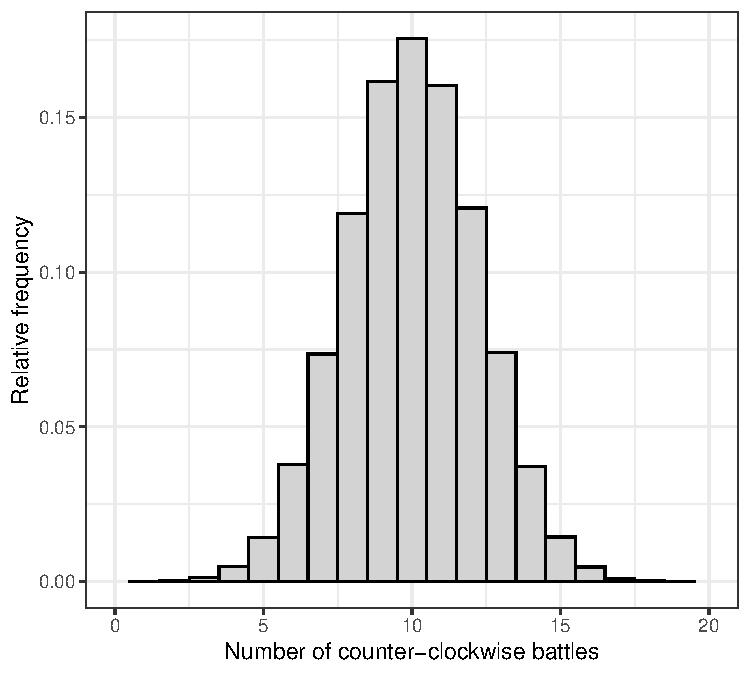
\includegraphics{BIOL202_files/figure-latex/unnamed-chunk-60-1.pdf}
\caption{\label{fig:unnamed-chunk-60}Approximate null distribution for the damselfly study, with n = 20 trials, and probability of success = 0.5 in each trial. Data are from 100000 repetitions.}
\end{figure}

The null distribution above shows us that if the null hypothesis was true, the most probable outcome would be 10 counter-clockwise battles out of 20. But other outcomes are of course possible, with decreasing probability towards zero and twenty.

\subsection{\texorpdfstring{Calculating the \emph{P}-value}{Calculating the P-value}}\label{calc_p}

The \textbf{\emph{P}-value} is defined as the probability of observing an outcome as extreme or more extreme as the observed value of the test statistic, if the null hypothesis were true.

In our damselfly study, we observed 17 out of 20 battles to be in the counter-clockwise direction.

We can calculate a \textbf{\emph{P}-value} as follows:

\begin{itemize}
\tightlist
\item
  first calculate the fraction of the \ensuremath{10^{5}} values in our null distribution that are equal to or greater than our observed test statistic value (here, 17)
\item
  if we have a 2-tailed alternative hypothesis, then we also need to calculate the fraction of the \ensuremath{10^{5}} values in our null distribution that are less than or equal to 3, which is the mirror number to 17 in the opposite side of the distribution.
\end{itemize}

Although our approximate null distribution that we created looks quite symmetrical, it's best not to assume it is (because recall that we generated this via simulation). Therefore we don't simply multiply the first value we calculate above by two. In future tutorials you'll learn how to calculate \textbf{\emph{P}-values} using built-in R functions and theoretical probability distributions.

In the \hyperref[coding_basics]{Introductory R Tutorials} you learned how to use \textbf{logical comparison operators} such as \texttt{\textgreater{}} and \texttt{\textless{}=}. We'll use these here.

Let's find out how many values within the variable \texttt{n} in our \texttt{null\_distribution} tibble are less than or equal to 3, or greater than or equal to 17:

\begin{Shaded}
\begin{Highlighting}[]
\NormalTok{null\_distribution }\SpecialCharTok{\%\textgreater{}\%}
  \FunctionTok{filter}\NormalTok{(n }\SpecialCharTok{\textless{}=} \DecValTok{3} \SpecialCharTok{|}\NormalTok{ n }\SpecialCharTok{\textgreater{}=} \DecValTok{17}\NormalTok{) }\SpecialCharTok{\%\textgreater{}\%}
  \FunctionTok{nrow}\NormalTok{() }
\end{Highlighting}
\end{Shaded}

\begin{verbatim}
## [1] 254
\end{verbatim}

This code uses the \texttt{filter} function to return only the rows that meet the condition specified: the ``n'' variable value less than or equal to 3, OR (using the ``\textbar{}'' symbol) greater than or equal to 17.

The \texttt{nrow} function then simply counts the number of rows in the resulting (filtered) tibble.

We see that among the \ensuremath{10^{5}} replications we ran, 254 yielded outcomes in which 3 or fewer, or 17 or more out of 20 battles were in the counter-clockwise direction.

To calculate the \emph{P}-value, we need to divide the 254 by the total number of reps that we conducted, here \ensuremath{10^{5}}.

\begin{Shaded}
\begin{Highlighting}[]
\NormalTok{null\_distribution }\SpecialCharTok{\%\textgreater{}\%}
  \FunctionTok{filter}\NormalTok{(n }\SpecialCharTok{\textless{}=} \DecValTok{3} \SpecialCharTok{|}\NormalTok{ n }\SpecialCharTok{\textgreater{}=} \DecValTok{17}\NormalTok{) }\SpecialCharTok{\%\textgreater{}\%}
  \FunctionTok{nrow}\NormalTok{() }\SpecialCharTok{/}\NormalTok{ num.reps}
\end{Highlighting}
\end{Shaded}

\begin{verbatim}
## [1] 0.00254
\end{verbatim}

So the \textbf{\emph{P}-value} associated with our observed test statistic is 0.00254.

\subsection{Writing a concluding statement}\label{concluding_statement}

It is important to write a concluding statement that talks about the actual findings of the study. For example:

In their territorial bouts, the damselflies flew in a counter-clockwise direction significantly more than expected (17 counter-clockwise flights out of \emph{n} = 20 trials; \emph{P}-value = 0.003). This is consistent with the idea that there is ``handedness'' in this population of \emph{C. maculata}.

It is also crucial that you report the sample size (here, number of random trials), the value of the observed test statistic (here 17), and the associated \textbf{\emph{P}-value}. Note we rounded the \textbf{\emph{P}-value} to three decimal places.

When we learn new types of statistical test, we'll adjust our concluding statements accordingly.

\begin{enumerate}
\def\labelenumi{\arabic{enumi}.}
\tightlist
\item
  Using this tutorial as a guide, try to repeat all the steps of a hypothesis test for Example 6.2 in the text book (concerning handedness in toads).
\end{enumerate}

\chapter{Analyzing a single categorical variable}\label{single_cat}

\textbf{Tutorial learning objectives}

\begin{itemize}
\tightlist
\item
  Learn how to calculate a standard error for a proportion
\item
  Learn how to calculate a confidence interval for a proportion
\item
  Learn about the binomial distribution and the \texttt{dbinom} function
\item
  Learn how to test hypotheses about a proportion using the \textbf{binomial test}
\item
  Learn an example of the confidence interval approach to hypothesis testing
\item
  Learn how to conduct a \textbf{\(\chi\)\textsuperscript{2} goodness of fit test} using a proportional model
\end{itemize}

\section{Load packages and import data}\label{singcat_packages_data}

Load the \texttt{tidyverse}, \texttt{skimr}, \texttt{naniar}, \texttt{knitr}, and \texttt{janitor} packages:

\begin{Shaded}
\begin{Highlighting}[]
\FunctionTok{library}\NormalTok{(tidyverse)}
\FunctionTok{library}\NormalTok{(skimr)}
\FunctionTok{library}\NormalTok{(naniar)}
\FunctionTok{library}\NormalTok{(knitr)}
\FunctionTok{library}\NormalTok{(janitor)}
\end{Highlighting}
\end{Shaded}

We will also need a new package called \texttt{binom}, so install that package using the procedure you \hyperref[package_install]{previously learned}, then load it:

\begin{Shaded}
\begin{Highlighting}[]
\FunctionTok{library}\NormalTok{(binom)}
\end{Highlighting}
\end{Shaded}

Import the \texttt{damselfly.csv} data set we used in the preceding \hyperref[hypothesis]{tutorial}, and also the \texttt{birds.csv} dataset we used in an earlier \hyperref[vis_describe]{tutorial}.

\begin{Shaded}
\begin{Highlighting}[]
\NormalTok{damselfly }\OtherTok{\textless{}{-}} \FunctionTok{read\_csv}\NormalTok{(}\StringTok{"https://raw.githubusercontent.com/ubco{-}biology/BIOL202/main/data/damselfly.csv"}\NormalTok{)}
\end{Highlighting}
\end{Shaded}

\begin{verbatim}
## Rows: 20 Columns: 1
## -- Column specification --------------------------------------------------------
## Delimiter: ","
## chr (1): direction
## 
## i Use `spec()` to retrieve the full column specification for this data.
## i Specify the column types or set `show_col_types = FALSE` to quiet this message.
\end{verbatim}

\begin{Shaded}
\begin{Highlighting}[]
\NormalTok{birds }\OtherTok{\textless{}{-}} \FunctionTok{read\_csv}\NormalTok{(}\StringTok{"https://raw.githubusercontent.com/ubco{-}biology/BIOL202/main/data/birds.csv"}\NormalTok{)}
\end{Highlighting}
\end{Shaded}

\begin{verbatim}
## Rows: 86 Columns: 1
## -- Column specification --------------------------------------------------------
## Delimiter: ","
## chr (1): type
## 
## i Use `spec()` to retrieve the full column specification for this data.
## i Specify the column types or set `show_col_types = FALSE` to quiet this message.
\end{verbatim}

Recall what the damselfly dataset looks like:

\begin{Shaded}
\begin{Highlighting}[]
\NormalTok{damselfly}
\end{Highlighting}
\end{Shaded}

\begin{verbatim}
## # A tibble: 20 x 1
##    direction        
##    <chr>            
##  1 clockwise        
##  2 counter_clockwise
##  3 counter_clockwise
##  4 clockwise        
##  5 counter_clockwise
##  6 counter_clockwise
##  7 counter_clockwise
##  8 counter_clockwise
##  9 counter_clockwise
## 10 counter_clockwise
## 11 counter_clockwise
## 12 clockwise        
## 13 counter_clockwise
## 14 counter_clockwise
## 15 counter_clockwise
## 16 counter_clockwise
## 17 counter_clockwise
## 18 counter_clockwise
## 19 counter_clockwise
## 20 counter_clockwise
\end{verbatim}

The data show the predominant direction (either clockwise or counter-clockwise) of 20 circular battles between male damseflies.

And remind yourself what the birds dataset looks like:

\begin{Shaded}
\begin{Highlighting}[]
\NormalTok{birds}
\end{Highlighting}
\end{Shaded}

\begin{verbatim}
## # A tibble: 86 x 1
##    type     
##    <chr>    
##  1 Waterfowl
##  2 Predatory
##  3 Predatory
##  4 Waterfowl
##  5 Shorebird
##  6 Waterfowl
##  7 Waterfowl
##  8 Songbird 
##  9 Predatory
## 10 Waterfowl
## # i 76 more rows
\end{verbatim}

These data describe the category of bird (variable ``type'' that has 4 different categories) for a random sample of 86 birds sampled at a marsh habitat.

\section{Estimating proportions}\label{estproportions}

Recall that the key descriptor for a categorical variable is a \textbf{proportion}. And when we wish to draw inferences about a categorical attribute within a population of interest, we take a random sample from the population to \emph{estimate} the true proportion \({p}\) of the population with that attribute. Our estimate is denoted \(\hat{p}\).

In a \hyperref[vis_cat_freq_table]{previous tutorial} we used the ``birds'' dataset to practice creating a ``frequency table'' that showed the \emph{relative frequencies} of birds falling in each category of the categorical variable ``type''. These relative frequencies are equivalent to their respective proportions.

So, for the birds dataset, let's produce a frequency table, but instead of using the term ``relative frequency'' we'll use ``p\_hat'' to denote that this is our estimate of the proportion of birds in that category.

We'll put the output in an object ``bird.freq.table'' then we'll display it after:

\begin{Shaded}
\begin{Highlighting}[]
\NormalTok{bird.freq.table }\OtherTok{\textless{}{-}}\NormalTok{ birds }\SpecialCharTok{\%\textgreater{}\%}
  \FunctionTok{count}\NormalTok{(type, }\AttributeTok{sort =} \ConstantTok{TRUE}\NormalTok{) }\SpecialCharTok{\%\textgreater{}\%} 
  \FunctionTok{mutate}\NormalTok{(}\AttributeTok{p\_hat =}\NormalTok{ n }\SpecialCharTok{/} \FunctionTok{sum}\NormalTok{(n))}
\end{Highlighting}
\end{Shaded}

Now show the table:

\begin{Shaded}
\begin{Highlighting}[]
\FunctionTok{kable}\NormalTok{(bird.freq.table, }\AttributeTok{digits =} \DecValTok{4}\NormalTok{)}
\end{Highlighting}
\end{Shaded}

type

n

p\_hat

Waterfowl

43

0.5000

Predatory

29

0.3372

Shorebird

8

0.0930

Songbird

6

0.0698

We can see that the proportion of birds at the marsh that belong to the ``Predatory'' category is about 0.34. Assuming we had a good random sample, this is our best estimate of the true proportion of marsh birds that are predatory.

Being an estimate, however, we need to attach some measure of uncertainty to it.

In a previous tutorial we learned how to calculate the \hyperref[sem_page]{standard error} and rule-of-thumb 95\% \hyperref[confint_rough]{confidence interval} for the \textbf{mean}.

Here we'll learn how to calculate these measures of uncertainty for a \textbf{proportion}.

\subsection{Standard error for a proportion}\label{sterr_prop}

Here's the equation for the standard error for the proportion:

\[SE_\hat{p} = \sqrt\frac{\hat{p}(1-\hat{p})}{n}\]

Let's use the ``birds'' dataset to demonstrate the calculation.

Let's re-create the table again:

\begin{Shaded}
\begin{Highlighting}[]
\NormalTok{bird.freq.table }\OtherTok{\textless{}{-}}\NormalTok{ birds }\SpecialCharTok{\%\textgreater{}\%}
  \FunctionTok{count}\NormalTok{(type, }\AttributeTok{sort =} \ConstantTok{TRUE}\NormalTok{) }\SpecialCharTok{\%\textgreater{}\%} 
  \FunctionTok{mutate}\NormalTok{(}\AttributeTok{p\_hat =}\NormalTok{ n }\SpecialCharTok{/} \FunctionTok{sum}\NormalTok{(n))}
\end{Highlighting}
\end{Shaded}

Show the table:

\begin{Shaded}
\begin{Highlighting}[]
\FunctionTok{kable}\NormalTok{(bird.freq.table, }\AttributeTok{digits =} \DecValTok{4}\NormalTok{)}
\end{Highlighting}
\end{Shaded}

type

n

p\_hat

Waterfowl

43

0.5000

Predatory

29

0.3372

Shorebird

8

0.0930

Songbird

6

0.0698

That table does show us our estimate of the proportion of birds that are predatory. We'll isolate that value later.

But we also need to get the total sample size, i.e.~the total number of birds sampled.

To do this, we need to make sure not to count any missing values, and we can use the \texttt{n\_complete} function from the \texttt{naniar} package:

\begin{Shaded}
\begin{Highlighting}[]
\NormalTok{birds.sampsize }\OtherTok{\textless{}{-}}\NormalTok{ birds }\SpecialCharTok{\%\textgreater{}\%}
  \FunctionTok{select}\NormalTok{(type) }\SpecialCharTok{\%\textgreater{}\%}
  \FunctionTok{n\_complete}\NormalTok{()}
\end{Highlighting}
\end{Shaded}

In the preceding code:

\begin{itemize}
\tightlist
\item
  We first ensure the output will be put in a new object called ``birds.sampsize''
\item
  We provide the tibble \texttt{birds}, which is what is fed to the subsequent code
\item
  We then use \texttt{select} to select the variable of interest ``type''
\item
  We then use the \texttt{n\_complete} function to get the total number of non-missing observations in the variable.
\end{itemize}

Now let's see what the outcome was:

\begin{Shaded}
\begin{Highlighting}[]
\NormalTok{birds.sampsize}
\end{Highlighting}
\end{Shaded}

\begin{verbatim}
## [1] 86
\end{verbatim}

In previous tutorials we used a bit more cumbersome way to calculate the total number of complete observations in a variable. The \texttt{n\_complete} function will simplify things.

Now that we have \emph{n} (above), stored in the object ``birds.sampsize'', we need to extract the ``p\_hat'' value associated with the ``Predatory'' category, and we'll store this in an object called ``pred.phat'':

\begin{Shaded}
\begin{Highlighting}[]
\NormalTok{pred.phat }\OtherTok{\textless{}{-}}\NormalTok{ bird.freq.table }\SpecialCharTok{\%\textgreater{}\%}
  \FunctionTok{filter}\NormalTok{(type }\SpecialCharTok{==} \StringTok{"Predatory"}\NormalTok{) }\SpecialCharTok{\%\textgreater{}\%}
  \FunctionTok{select}\NormalTok{(p\_hat)}
\end{Highlighting}
\end{Shaded}

In the preceding chunk we:

\begin{itemize}
\tightlist
\item
  assign our output to an object ``pred.phat''
\item
  use the \texttt{filter} function to get the rows where the ``type'' variable is equal to the ``Predatory'' category
\item
  use the \texttt{select} function to return (select) the ``p\_hat'' variable only
\end{itemize}

Let's look at what this produced:

\begin{Shaded}
\begin{Highlighting}[]
\NormalTok{pred.phat}
\end{Highlighting}
\end{Shaded}

\begin{verbatim}
## # A tibble: 1 x 1
##    p_hat
##    <dbl>
## 1 0.3372
\end{verbatim}

So this produced a tibble called ``pred.phat'' with a variable ``p\_hat'', and it has one value - our proportion estimate \(\hat{p}\).

\textbf{TIP}: We could have calculated and isolated the ``P-hat'' value for predatory birds all in one go, using the following code:

\begin{Shaded}
\begin{Highlighting}[]
\NormalTok{pred.phat }\OtherTok{\textless{}{-}}\NormalTok{ birds }\SpecialCharTok{\%\textgreater{}\%}
  \FunctionTok{count}\NormalTok{(type, }\AttributeTok{sort =} \ConstantTok{TRUE}\NormalTok{) }\SpecialCharTok{\%\textgreater{}\%} 
  \FunctionTok{mutate}\NormalTok{(}\AttributeTok{p\_hat =}\NormalTok{ n }\SpecialCharTok{/} \FunctionTok{sum}\NormalTok{(n)) }\SpecialCharTok{\%\textgreater{}\%}
  \FunctionTok{filter}\NormalTok{(type }\SpecialCharTok{==} \StringTok{"Predatory"}\NormalTok{) }\SpecialCharTok{\%\textgreater{}\%}
  \FunctionTok{select}\NormalTok{(p\_hat)}
\end{Highlighting}
\end{Shaded}

That demonstrates the power of the pipe approach!

OK, now we're ready to calculate \(SE_\hat{p} = \sqrt\frac{\hat{p}(1-\hat{p})}{n}\)

Here's how we do this using basic R syntax, recalling that our ``n'' (86 birds total) is stored in the object ``birds.sampsize''.

We'll store the value in a new object called ``SE\_phat'':

\begin{Shaded}
\begin{Highlighting}[]
\NormalTok{SE\_phat }\OtherTok{\textless{}{-}} \FunctionTok{sqrt}\NormalTok{(pred.phat }\SpecialCharTok{*}\NormalTok{ (}\DecValTok{1} \SpecialCharTok{{-}}\NormalTok{ pred.phat) }\SpecialCharTok{/}\NormalTok{ birds.sampsize)}
\end{Highlighting}
\end{Shaded}

And now see what the value is:

\begin{Shaded}
\begin{Highlighting}[]
\NormalTok{SE\_phat}
\end{Highlighting}
\end{Shaded}

\begin{verbatim}
##       p_hat
## 1 0.0509787
\end{verbatim}

\textbf{Reporting the proportion and standard error}

To properly report a proportion estimate along with its standard error, we need to know how to produce a ``plus/minus'' symbol in markdown.

Here's what you type in the regular text area of your markdown document (not in a code chunk).

\begin{verbatim}
$\pm$
\end{verbatim}

The \texttt{\$\textbackslash{}pm\$} is the syntax for a plus-minus symbol. More symbols can be found at this \href{https://rpruim.github.io/s341/S19/from-class/MathinRmd.html}{website}.

And so you insert that text in between your estimate \(\hat{p}\) and the \(SE_\hat{p}\), as such: 0.34 \(\pm\) 0.051.

\subsection{Confidence interval for a proportion}\label{confint_prop}

Although a number of options are available for calculating a confidence interval for a proportion, we'll use the \emph{Agresti-Coull} method, as it has desirable properties:

\[p' \pm 1.96\cdot \sqrt\frac{p'(1-p')}{N+4}\] where \[p' = \frac{X+2}{n+4}\]

The \textbf{margin of error} from the above equation is this part:

\[1.96\cdot \sqrt\frac{p'(1-p')}{N+4}\]

This margin of error is the value that we \emph{subtract} to our proportion estimate \(\hat{p}\) to get the \textbf{lower 95\% confidence limit}, and we \emph{add} that value to our proportion estimate \(\hat{p}\) to get the \textbf{upper 95\% confidence limit}.

We'll again use the ``birds'' data, and the estimated proportion of birds that are predatory.

Let's again calculate the sample size of birds:

\begin{Shaded}
\begin{Highlighting}[]
\NormalTok{birds.sampsize }\OtherTok{\textless{}{-}}\NormalTok{ birds }\SpecialCharTok{\%\textgreater{}\%}
  \FunctionTok{select}\NormalTok{(type) }\SpecialCharTok{\%\textgreater{}\%}
  \FunctionTok{n\_complete}\NormalTok{()}
\end{Highlighting}
\end{Shaded}

And here's the frequency table we constructed:

\begin{Shaded}
\begin{Highlighting}[]
\NormalTok{bird.freq.table }\OtherTok{\textless{}{-}}\NormalTok{ birds }\SpecialCharTok{\%\textgreater{}\%}
  \FunctionTok{count}\NormalTok{(type, }\AttributeTok{sort =} \ConstantTok{TRUE}\NormalTok{) }\SpecialCharTok{\%\textgreater{}\%} 
  \FunctionTok{mutate}\NormalTok{(}\AttributeTok{p\_hat =}\NormalTok{ n }\SpecialCharTok{/} \FunctionTok{sum}\NormalTok{(n))}
\end{Highlighting}
\end{Shaded}

Show the table:

\begin{Shaded}
\begin{Highlighting}[]
\NormalTok{bird.freq.table}
\end{Highlighting}
\end{Shaded}

\begin{verbatim}
## # A tibble: 4 x 3
##   type          n   p_hat
##   <chr>     <int>   <dbl>
## 1 Waterfowl    43 0.5    
## 2 Predatory    29 0.3372 
## 3 Shorebird     8 0.09302
## 4 Songbird      6 0.06977
\end{verbatim}

Looking at the formula for the \emph{Agresti-Coull} confidence interal, we see that we need \emph{X} - the number of ``successes'', which in our case is the number of birds in the category ``Predatory''. This is provided in our table above. So let's extract that information.

We'll store our value of ``X'' in a new object called ``bird.X'':

\begin{Shaded}
\begin{Highlighting}[]
\NormalTok{bird.X }\OtherTok{\textless{}{-}}\NormalTok{ bird.freq.table }\SpecialCharTok{\%\textgreater{}\%}
  \FunctionTok{filter}\NormalTok{(type }\SpecialCharTok{==} \StringTok{"Predatory"}\NormalTok{) }\SpecialCharTok{\%\textgreater{}\%}
  \FunctionTok{select}\NormalTok{(n)}
\end{Highlighting}
\end{Shaded}

Now let's see the output:

\begin{Shaded}
\begin{Highlighting}[]
\NormalTok{bird.X}
\end{Highlighting}
\end{Shaded}

\begin{verbatim}
## # A tibble: 1 x 1
##       n
##   <int>
## 1    29
\end{verbatim}

Unlike the standard error calculation, for which we did actual math using R, for the confidence interval we'll make use of the \texttt{binom.confint} function from the \texttt{binom} package. Have a look at the help page:

\begin{verbatim}
?binom.confint
\end{verbatim}

The function takes a handful of arguments, including the value of \emph{X}, the number of trials \emph{n}, the confidence level we wish to use (typically 0.95 corresponding to a 95\% confidence interval), and the method one wishes to use.

Let's try it out using our bird data.

The one catch in the code below is that we can't simply provide the name of our ``bird.X'' object to provide the value of \emph{X} for the \texttt{binom.confint} function; instead we need to specify that the value we want to use is stored in the variable called ``n'' within the ``bird.X'' object. Thus, we use \texttt{bird.X\$n}. The dollar sign allows us to specify a specific variable within the tibble.

Then, we use ``ac'' to specify the ``Agresti-Coull'' methods.

We'll assing our output to a new object called ``confint.results'':

\begin{Shaded}
\begin{Highlighting}[]
\NormalTok{confint.results }\OtherTok{\textless{}{-}} \FunctionTok{binom.confint}\NormalTok{(}\AttributeTok{x =}\NormalTok{ bird.X}\SpecialCharTok{$}\NormalTok{n, }\AttributeTok{n =}\NormalTok{ birds.sampsize, }\AttributeTok{conf.level =} \FloatTok{0.95}\NormalTok{, }\AttributeTok{methods =} \StringTok{"ac"}\NormalTok{)}
\end{Highlighting}
\end{Shaded}

Have a look at the output using the \texttt{kable} function to make it nicer looking:

\begin{Shaded}
\begin{Highlighting}[]
\FunctionTok{kable}\NormalTok{(confint.results, }\AttributeTok{digits =} \DecValTok{4}\NormalTok{)}
\end{Highlighting}
\end{Shaded}

method

x

n

mean

lower

upper

agresti-coull

29

86

0.3372

0.2459

0.4424

The function provides us with the values of \emph{X}, \emph{n}, the proportion estimate (strangely called ``mean''), and the lower and upper confidence limits.

\textbf{Reporting the confidence interval for a proportion}

The appropriate way to report the confidence interval is as follows:

The 95\% Agresti-Coull confidence interval is: 0.246 \(< {p} <\) 0.442.

\begin{enumerate}
\def\labelenumi{\arabic{enumi}.}
\tightlist
\item
  What is the best estimate of the proportion of the marsh birds that belong to the ``Shorebird'' category? What is the standard error of the proportion, and the 95\% Agresti-Coull confidence interval?
\end{enumerate}

\section{Binomial distribution}\label{binomdist}

The binomial distribution provides the probability distribution for the number of ``successes'' in a fixed number of independent trials, when the probability of success is the same in each trial.

Here's the formula:

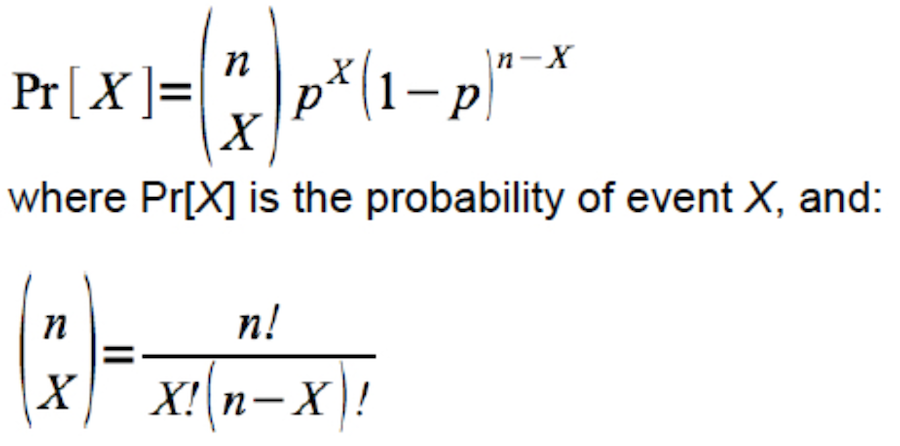
\includegraphics[width=12.5in]{./more/binomial_equation}

It turns out there's a handy function \texttt{dbinom} (available in the base R package) that will calculate the exact probability associated with any particular outcome for a random trial with a given sample space (set of outcomes) and probability of success. It uses the equation shown above.

Check the help file for the function:

\begin{verbatim}
?dbinom
\end{verbatim}

\textbf{Dice example}

Imagine rolling a fair, 6-sided die \emph{n} = 6 times (six random trials). Let's consider rolling a ``4'' a ``success''.

What is the probability of observing two fours (i.e.~two successes) in our 6 rolls of the die (random trials)?

We have \emph{X} = 2 (the number of successes), \emph{p} = 1/6 (the probability of a success in each trial), and \emph{n} = 6 (the number of trials).

Here's the code, where ``x'' represents our ``\emph{X}'', ``size'' represents the number of trials (``\emph{n}''), and ``prob'' is the probability of success in each trial (here, 1/6).

We'll create an object to hold the number of trials we wish to use first:

\begin{Shaded}
\begin{Highlighting}[]
\NormalTok{num.trials }\OtherTok{\textless{}{-}} \DecValTok{6}
\FunctionTok{dbinom}\NormalTok{(}\AttributeTok{x =} \DecValTok{2}\NormalTok{, }\AttributeTok{size =}\NormalTok{ num.trials, }\AttributeTok{prob =} \DecValTok{1}\SpecialCharTok{/}\DecValTok{6}\NormalTok{)}
\end{Highlighting}
\end{Shaded}

\begin{verbatim}
## [1] 0.2009388
\end{verbatim}

Thus, the probability of rolling two fours (i.e.~having 2 successes) out of 6 rolls of the dice is about 0.201.

In order to get the probabilities associated with \emph{each} possible outcome (i.e.~0 through 6 successes), we use the code shown in the chunk below.

\begin{Shaded}
\begin{Highlighting}[]
\NormalTok{exact.probs}\FloatTok{.6} \OtherTok{\textless{}{-}} \FunctionTok{tibble}\NormalTok{(}
  \AttributeTok{X =} \DecValTok{0}\SpecialCharTok{:}\NormalTok{num.trials,}
  \AttributeTok{probs =} \FunctionTok{dbinom}\NormalTok{(}\AttributeTok{x =} \DecValTok{0}\SpecialCharTok{:}\NormalTok{num.trials, }\AttributeTok{size =}\NormalTok{ num.trials, }\AttributeTok{prob =} \DecValTok{1}\SpecialCharTok{/}\DecValTok{6}\NormalTok{)}
\NormalTok{  )}
\NormalTok{exact.probs}\FloatTok{.6}
\end{Highlighting}
\end{Shaded}

\begin{verbatim}
## # A tibble: 7 x 2
##       X      probs
##   <int>      <dbl>
## 1     0 0.3349    
## 2     1 0.4019    
## 3     2 0.2009    
## 4     3 0.05358   
## 5     4 0.008038  
## 6     5 0.0006430 
## 7     6 0.00002143
\end{verbatim}

Above we created a new tibble object (using the function \texttt{tibble}) called ``exact.probs.6'', with a variable ``X'' that holds each of the possible outcomes (X = 0 through 6 or the number of trials), and ``probs'' that holds the probability of each outcome, calculated using the \texttt{dbinom} function:

See that the \texttt{dbinom} function will accept a vector of values of \texttt{x}, for which the associated probabilities are calculated.

Now let's use these exact probabilities to create a barplot showing an exact, discrete probability distribution, corresponding to the binomial distribution with a sample size (number of trials) of \emph{n} = 6 and a probability of success \emph{p} = 1/6:

\begin{Shaded}
\begin{Highlighting}[]
\FunctionTok{ggplot}\NormalTok{(exact.probs}\FloatTok{.6}\NormalTok{, }\FunctionTok{aes}\NormalTok{(}\AttributeTok{y =}\NormalTok{ probs, }\AttributeTok{x =}\NormalTok{ X)) }\SpecialCharTok{+}
  \FunctionTok{geom\_bar}\NormalTok{(}\AttributeTok{stat =} \StringTok{"identity"}\NormalTok{, }\AttributeTok{fill =} \StringTok{"lightgrey"}\NormalTok{, }\AttributeTok{colour =} \StringTok{"black"}\NormalTok{) }\SpecialCharTok{+}
  \FunctionTok{xlab}\NormalTok{(}\StringTok{"Number of successes (X)"}\NormalTok{) }\SpecialCharTok{+}
  \FunctionTok{ylab}\NormalTok{(}\StringTok{"Pr[X]"}\NormalTok{) }\SpecialCharTok{+}
  \FunctionTok{theme\_bw}\NormalTok{()}
\end{Highlighting}
\end{Shaded}

\begin{figure}
\centering
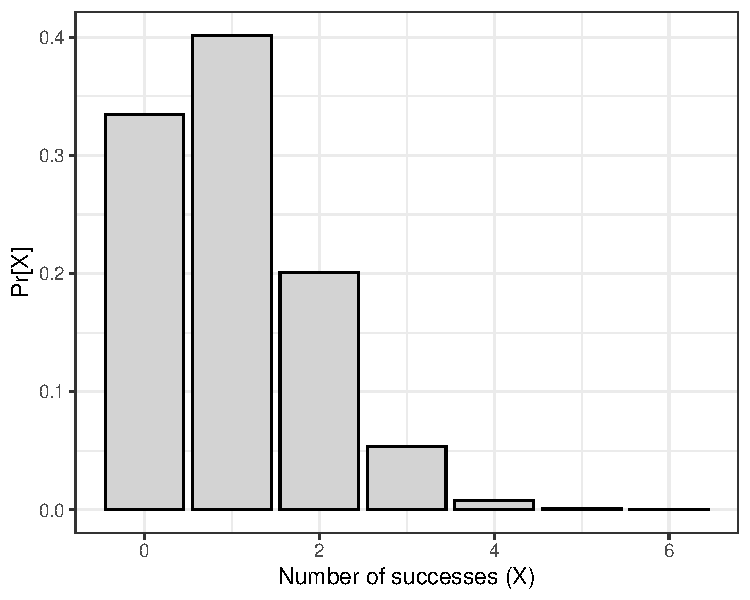
\includegraphics{BIOL202_files/figure-latex/unnamed-chunk-66-1.pdf}
\caption{\label{fig:unnamed-chunk-66}Probability of obtaining X successes out of 6 random trials, with probability of success = 1/6.}
\end{figure}

What if we wished to calculate the probability of getting \emph{at least} two fours in our 6 rolls of the dice?

Consult the bar chart above. Recall that ``rolling a 4'' is our definition of a ``success'' (it could have been ``rolling a 1'', or ``rolling a 5'' - these all result in the same calculation). Thus to calculate the probability of getting at least 2 successes we need to sum up the probabilities associated with getting 2, 3, 4, 5, and 6 successes.

We can do this using the following R code:

\begin{Shaded}
\begin{Highlighting}[]
\NormalTok{probs}\FloatTok{.2}\NormalTok{\_to\_6 }\OtherTok{\textless{}{-}} \FunctionTok{dbinom}\NormalTok{(}\AttributeTok{x =} \DecValTok{2}\SpecialCharTok{:}\NormalTok{num.trials, }\AttributeTok{size =}\NormalTok{ num.trials, }\AttributeTok{prob =} \DecValTok{1}\SpecialCharTok{/}\DecValTok{6}\NormalTok{)}
\FunctionTok{sum}\NormalTok{(probs}\FloatTok{.2}\NormalTok{\_to\_6)}
\end{Highlighting}
\end{Shaded}

\begin{verbatim}
## [1] 0.2632245
\end{verbatim}

Note that we ask the \texttt{dbinom} function to do the calculation for each of the \texttt{2:num.trials} outcomes of interest. We store these calculated probabilities in a new object ``probs.2\_to\_6''.

Then, we use the \texttt{sum} function to sum up the probabilities within that object.

The resulting value of 0.2632245 looks about right based on our bar chart!

\begin{center}\rule{0.5\linewidth}{0.5pt}\end{center}

Now let's increase the number of trials to \emph{n} = 15, and compare the distribution to that observed using \emph{n} = 6:

\begin{Shaded}
\begin{Highlighting}[]
\NormalTok{num.trials }\OtherTok{\textless{}{-}} \DecValTok{15}
\NormalTok{exact.probs}\FloatTok{.15} \OtherTok{\textless{}{-}} \FunctionTok{tibble}\NormalTok{(}
  \AttributeTok{X =} \DecValTok{0}\SpecialCharTok{:}\NormalTok{num.trials,}
  \AttributeTok{probs =} \FunctionTok{dbinom}\NormalTok{(}\AttributeTok{x =} \DecValTok{0}\SpecialCharTok{:}\NormalTok{num.trials, }\AttributeTok{size =}\NormalTok{ num.trials, }\AttributeTok{prob =} \DecValTok{1}\SpecialCharTok{/}\DecValTok{6}\NormalTok{)}
\NormalTok{  )}
\NormalTok{exact.probs}\FloatTok{.15}
\end{Highlighting}
\end{Shaded}

\begin{verbatim}
## # A tibble: 16 x 2
##        X     probs
##    <int>     <dbl>
##  1     0 6.491e- 2
##  2     1 1.947e- 1
##  3     2 2.726e- 1
##  4     3 2.363e- 1
##  5     4 1.418e- 1
##  6     5 6.237e- 2
##  7     6 2.079e- 2
##  8     7 5.346e- 3
##  9     8 1.069e- 3
## 10     9 1.663e- 4
## 11    10 1.996e- 5
## 12    11 1.814e- 6
## 13    12 1.210e- 7
## 14    13 5.583e- 9
## 15    14 1.595e-10
## 16    15 2.127e-12
\end{verbatim}

Now plot the binomial probability distribution:

\begin{Shaded}
\begin{Highlighting}[]
\FunctionTok{ggplot}\NormalTok{(exact.probs}\FloatTok{.15}\NormalTok{, }\FunctionTok{aes}\NormalTok{(}\AttributeTok{y =}\NormalTok{ probs, }\AttributeTok{x =}\NormalTok{ X)) }\SpecialCharTok{+}
  \FunctionTok{geom\_bar}\NormalTok{(}\AttributeTok{stat =} \StringTok{"identity"}\NormalTok{, }\AttributeTok{fill =} \StringTok{"lightgrey"}\NormalTok{, }\AttributeTok{colour =} \StringTok{"black"}\NormalTok{) }\SpecialCharTok{+}
  \FunctionTok{xlab}\NormalTok{(}\StringTok{"Number of successes (X)"}\NormalTok{) }\SpecialCharTok{+}
  \FunctionTok{ylab}\NormalTok{(}\StringTok{"Pr[X]"}\NormalTok{) }\SpecialCharTok{+}
  \FunctionTok{theme\_bw}\NormalTok{()}
\end{Highlighting}
\end{Shaded}

\begin{figure}
\centering
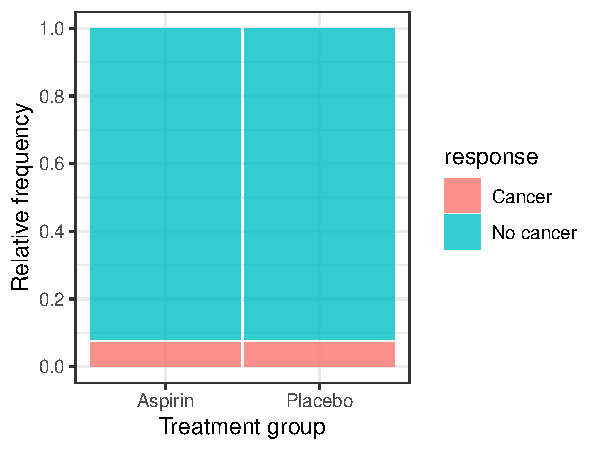
\includegraphics{BIOL202_files/figure-latex/unnamed-chunk-67-1.pdf}
\caption{\label{fig:unnamed-chunk-67}Probability of obtaining X successes out of 15 random trials, with probability of success = 1/6.}
\end{figure}

\begin{enumerate}
\def\labelenumi{\arabic{enumi}.}
\tightlist
\item
  Challenge: Binomial probabilities
\end{enumerate}

\begin{itemize}
\tightlist
\item
  Use the \texttt{dbinom} function to calculate the probability of rolling three ``2''s when rolling a fair six-sided die 20 times.
\item
  Produce a graph of a discrete probability distribution for this scenario: \emph{p} = 1/4, and \emph{n} = 12.
\end{itemize}

\section{Binomial test}\label{binom_test}

We previously learned about estimating proportions, and calculating measures of uncertainty for those estimates.

Now we'll learn a procedure for testing hypotheses about proportions.

For this example we'll use the \texttt{damselfly} dataset we used in the previous tutorial regarding \hyperref[hypothesis]{hypothesis tests}.

Recall that the researcher found that in 17 out of 20 circular battles (or ``bouts'') the damselflies flew in the counter-clockwise direction.

The question was: should this result be considered evidence of handedness in this population?

\begin{center}\rule{0.5\linewidth}{0.5pt}\end{center}

Take a moment to refresh your memory regarding the \hyperref[hyp_steps]{steps to hypothesis testing}.

We'll explain first how this is a test about a proportion.

Considering the question posed above, we need to first think about what we'd expect if there was truly \textbf{no} ``handedness'' in the population of damseflies. In this case, then we'd expect the circular battles to occur with equal frequency in both clockwise and counter-clockwise directions.

In other words, if there was no handedness, we'd expect the \emph{proportion} of battles that are counter-clockwise (the direction we'll arbitrarily call a ``success'') to equal \({p} = 0.5\).

\begin{itemize}
\tightlist
\item
  We'll use a \textbf{binomial test} here, because this is the \textbf{most appropriate (and powerful) test} when comparing the observed number of ``successes'' in a dataset to the number expected under a null hypothesis. Or put another way, we compare an observed \emph{proportion} of successes in a dataset to the proportion expected under a null hypothesis.
\end{itemize}

Let's devise an appropriate null and alternative hypothesis for this question.

\textbf{H\textsubscript{0}}: The proportion of damselfly battles in the population flown in the counter-clockwise direction is 0.5 (\(p_0 = 0.5\))

\textbf{H\textsubscript{A}}: The proportion of damselfly battles in the population flown in the counter-clockwise direction is not 0.5 (\(p_0 \ne 0.5\))

\begin{itemize}
\tightlist
\item
  We'll use an \(\alpha\) level of 0.05.\\
\item
  It is a two-tailed alternative hypothesis; there is no reason to eliminate the possibility that the damselflies exhibit right- or left-``handedness''
\item
  The binomial test assumes that the random trials were independent, and the probability of success was equal in each trial - we'll assume so!
\item
  We don't need a figure for this test
\item
  The test statistic is the number of battles that were flown predominantly in the counter-clockwise direction (the direction we arbitrarily chose as a ``success'').
\item
  The binomial test calculates an exact \emph{P}-value for us (using the \hyperref[binomdist]{binomial equation}), and we don't need to rely on an approximate null distribution, like we do for other tests.
\end{itemize}

Let's conduct the test now.

We use the \texttt{binom.test} function that is from the base R package.

\begin{verbatim}
?binom.test
\end{verbatim}

Let's show the code then explain after:

\begin{Shaded}
\begin{Highlighting}[]
\NormalTok{binom.test.results }\OtherTok{\textless{}{-}} \FunctionTok{binom.test}\NormalTok{(}\AttributeTok{x =} \DecValTok{17}\NormalTok{, }\AttributeTok{n =} \DecValTok{20}\NormalTok{, }\AttributeTok{p =} \FloatTok{0.5}\NormalTok{, }\AttributeTok{alternative =} \StringTok{"two.sided"}\NormalTok{)}
\end{Highlighting}
\end{Shaded}

\begin{itemize}
\tightlist
\item
  We create a new object ``binom.test.results'' to hold the results
\item
  the arguments for the \texttt{binom.test} function include the number of successes (x), the number of trials (n), the null hypothesized proportion (p), and we specify that the alternative hypothesis is ``two.sided'' - which is almost always the case
\end{itemize}

Now let's look at the output:

\begin{Shaded}
\begin{Highlighting}[]
\NormalTok{binom.test.results}
\end{Highlighting}
\end{Shaded}

\begin{verbatim}
## 
##  Exact binomial test
## 
## data:  17 and 20
## number of successes = 17, number of trials = 20, p-value = 0.002577
## alternative hypothesis: true probability of success is not equal to 0.5
## 95 percent confidence interval:
##  0.6210732 0.9679291
## sample estimates:
## probability of success 
##                   0.85
\end{verbatim}

The output from the binomial test includes the number of successes, the number of trials, and the calculated \emph{P}-value. It also includes a 95\% confidence interval for the proportion.

The confidence interval provided by this \texttt{binom.test} function is \emph{not} recommended. Rather, you should \textbf{ALWAYS} use the Agresti-Coull method to calculate a confidence interval for a proportion, as shown in the previous \hyperref[confint_prop]{tutorial}.

Let's now calculate the Agresti-Coull 95\% confidence interval for the proportion, as we learned previously, using the \texttt{binom.confint} function from the \texttt{binom} package:

\begin{Shaded}
\begin{Highlighting}[]
\NormalTok{damsel.confint.results }\OtherTok{\textless{}{-}} \FunctionTok{binom.confint}\NormalTok{(}\AttributeTok{x =} \DecValTok{17}\NormalTok{, }\AttributeTok{n =} \DecValTok{20}\NormalTok{, }\AttributeTok{conf.level =} \FloatTok{0.95}\NormalTok{, }\AttributeTok{methods =} \StringTok{"ac"}\NormalTok{)}
\end{Highlighting}
\end{Shaded}

And look at the output:

\begin{Shaded}
\begin{Highlighting}[]
\FunctionTok{kable}\NormalTok{(damsel.confint.results, }\AttributeTok{digits =} \DecValTok{4}\NormalTok{)}
\end{Highlighting}
\end{Shaded}

method

x

n

mean

lower

upper

agresti-coull

17

20

0.85

0.6312

0.9561

Now we have all the ingredients for a proper concluding statement.

This is an example of an appropriate concluding statement for a binomial test:

\begin{quote}
Counter-clockwise battles occurred with significantly greater frequency than expected (17 of 20 battles; observed proportion of counter-clockwise battles = 0.85; Binomial test; \emph{P}-value = 0.003; Agresti-Coull 95\% confidence interval: 0.631 \(< {p} <\) 0.956).
\end{quote}

\section{Confidence interval approach to hypothesis testing}\label{prophypconf}

In the preceding tutorial, we calculated the Agresti-Coull 95\% confidence interval for the proportion of damsefly battles flown in the counter-clockwise direction as: 0.631 \(< {p} <\) 0.956.

Given that the interval excludes (does not encompass) the null hypothesized proportion of \(p_0 = 0.5\), we can reject the null hypothesis.

In this case, the appropriate concluding statement would be:

\begin{quote}
Counter-clockwise battles occurred in a significantly higher proportion than 0.5 (observed proportion of counter-clockwise battles = 0.85; Agresti-Coull 95\% confidence interval: 0.631 \textless{} \({p}\) \textless{} 0.956.
\end{quote}

\begin{center}\rule{0.5\linewidth}{0.5pt}\end{center}

\begin{enumerate}
\def\labelenumi{\arabic{enumi}.}
\tightlist
\item
  \textbf{Binomial hypothesis test practice}: Using the present tutorial as a guide, use a \textbf{binomial test} to address the question posed in Example 6.2 in the text book (concerning handedness in toads). Be sure to include all the steps of a hypothesis test.
\end{enumerate}

\section{Goodness-of-fit tests}\label{GOF_test}

\textbf{This tutorial is under construction, and will not be covered in 2022}

In this tutorial, we continue to learn how to test hypotheses about a categorical variable.

We previously learned how to test a hypothesis about frequencies or proportions when the variable has only two categories of interest, i.e.~success and failure (a binary variable). We used a binomial test for this purpose. It is important to note, however, that even in cases where the variable has more than two categories (e.g.~hair colour: brown, black, blonde, red), one can define a particular category (e.g.~red hair) as a ``success'', and the remaining categories as failures, in which case we have simplified our variable to a binary categorical variable.

For testing hypotheses about frequencies or proportions when there are more than two categories, we use goodness of fit (GOF) tests. In general, these types of test evaluate how well an observed discrete frequency (or probability) distribution fits some hypothesized frequency distribution. We'll demonstrate this next.

\chapter{Analyzing associations between two categorical variables}\label{two_cat}

\textbf{Tutorial learning objectives}

\begin{itemize}
\tightlist
\item
  Learn about the odds Ratio for a \textbf{2 x 2} contingency table

  \begin{itemize}
  \tightlist
  \item
    Estimate the odds of an outcome\\
  \item
    Estimate the odds ratio
  \end{itemize}
\item
  Learn about the Fisher's Exact Test for a \textbf{2 x 2} contingency table

  \begin{itemize}
  \tightlist
  \item
    Hypothesis statement\\
  \item
    Display a Contingency table (review this \hyperref[vis2_cont_table]{tutorial})
  \item
    Display a Mosaic plot (review this \hyperref[mosaic_plot]{tutorial})
  \item
    Conduct the Fisher's Exact test\\
  \item
    Concluding statement
  \end{itemize}
\item
  Learn about the \(\chi\)\textsuperscript{2} Contingency Test on a \textbf{m x n} contingency table

  \begin{itemize}
  \tightlist
  \item
    Hypothesis statement\\
  \item
    Display a Contingency table (review this \hyperref[vis2_cont_table]{tutorial})
  \item
    Display a Mosaic plot (review this \hyperref[mosaic_plot]{tutorial})
  \item
    Check assumptions\\
  \item
    Get results of the test\\
  \item
    Concluding statement
  \end{itemize}
\end{itemize}

\section{Load packages and import data}\label{twocat_packages_data}

Load the \texttt{tidyverse}, \texttt{skimr}, \texttt{naniar}, \texttt{knitr}, \texttt{ggmosaic}, and \texttt{janitor} packages:

\begin{Shaded}
\begin{Highlighting}[]
\FunctionTok{library}\NormalTok{(tidyverse)}
\FunctionTok{library}\NormalTok{(skimr)}
\FunctionTok{library}\NormalTok{(naniar)}
\FunctionTok{library}\NormalTok{(knitr)}
\FunctionTok{library}\NormalTok{(ggmosaic)}
\FunctionTok{library}\NormalTok{(janitor)}
\end{Highlighting}
\end{Shaded}

We'll also need a new package called \texttt{epitools}, so install that now if you haven't done so.

\begin{Shaded}
\begin{Highlighting}[]
\FunctionTok{library}\NormalTok{(epitools)}
\end{Highlighting}
\end{Shaded}

\begin{verbatim}
## 
## Attaching package: 'epitools'
\end{verbatim}

\begin{verbatim}
## The following objects are masked from 'package:binom':
## 
##     binom.exact, binom.wilson
\end{verbatim}

We'll use two datasets described in the Whitlock \& Schluter text:

\begin{itemize}
\tightlist
\item
  the ``cancer.csv'' dataset (described in Example 9.2 in the text, page 238)
\item
  the ``worm.csv'' dataset (described in Example 9.4 in the text, page 246)
\end{itemize}

\begin{Shaded}
\begin{Highlighting}[]
\NormalTok{cancer }\OtherTok{\textless{}{-}} \FunctionTok{read\_csv}\NormalTok{(}\StringTok{"https://raw.githubusercontent.com/ubco{-}biology/BIOL202/main/data/cancer.csv"}\NormalTok{)}
\end{Highlighting}
\end{Shaded}

\begin{verbatim}
## Rows: 39876 Columns: 2
## -- Column specification --------------------------------------------------------
## Delimiter: ","
## chr (2): aspirinTreatment, response
## 
## i Use `spec()` to retrieve the full column specification for this data.
## i Specify the column types or set `show_col_types = FALSE` to quiet this message.
\end{verbatim}

\begin{Shaded}
\begin{Highlighting}[]
\NormalTok{worm }\OtherTok{\textless{}{-}} \FunctionTok{read\_csv}\NormalTok{(}\StringTok{"https://raw.githubusercontent.com/ubco{-}biology/BIOL202/main/data/worm.csv"}\NormalTok{)}
\end{Highlighting}
\end{Shaded}

\begin{verbatim}
## Rows: 141 Columns: 2
## -- Column specification --------------------------------------------------------
## Delimiter: ","
## chr (2): infection, fate
## 
## i Use `spec()` to retrieve the full column specification for this data.
## i Specify the column types or set `show_col_types = FALSE` to quiet this message.
\end{verbatim}

Take a look at the cancer dataset:

\begin{Shaded}
\begin{Highlighting}[]
\NormalTok{cancer }\SpecialCharTok{\%\textgreater{}\%}
 \FunctionTok{skim\_without\_charts}\NormalTok{()}
\end{Highlighting}
\end{Shaded}

(\#tab:cont\_datalook\_cancer)Data summary

Name

Piped data

Number of rows

39876

Number of columns

2

\_\_\_\_\_\_\_\_\_\_\_\_\_\_\_\_\_\_\_\_\_\_\_

Column type frequency:

character

2

\_\_\_\_\_\_\_\_\_\_\_\_\_\_\_\_\_\_\_\_\_\_\_\_

Group variables

None

\textbf{Variable type: character}

skim\_variable

n\_missing

complete\_rate

min

max

empty

n\_unique

whitespace

aspirinTreatment

0

1

7

7

0

2

0

response

0

1

6

9

0

2

0

And the worm dataset:

\begin{Shaded}
\begin{Highlighting}[]
\NormalTok{worm }\SpecialCharTok{\%\textgreater{}\%}
 \FunctionTok{skim\_without\_charts}\NormalTok{()}
\end{Highlighting}
\end{Shaded}

(\#tab:cont\_datalook\_worm)Data summary

Name

Piped data

Number of rows

141

Number of columns

2

\_\_\_\_\_\_\_\_\_\_\_\_\_\_\_\_\_\_\_\_\_\_\_

Column type frequency:

character

2

\_\_\_\_\_\_\_\_\_\_\_\_\_\_\_\_\_\_\_\_\_\_\_\_

Group variables

None

\textbf{Variable type: character}

skim\_variable

n\_missing

complete\_rate

min

max

empty

n\_unique

whitespace

infection

0

1

6

10

0

3

0

fate

0

1

5

9

0

2

0

Both datasets are formatted ``tidy'' format. For a refresher on this, review the \href{https://ubco-biology.github.io/Procedures-and-Guidelines/tidy-data.html}{Biology Procedures and Guidelines document} chapter on \textbf{Tidy data}.

\section{Fisher's Exact Test}\label{fishertest}

When testing for an association between two categorical variables, the most common test that is used is the \(\chi\)\textsuperscript{2} contingency test, which is described in the next section.

When the two categorical variables \emph{have exactly 2 categories each}, and thus yield a 2 x 2 contingency table, the \textbf{Fisher's Exact test} (a type of contingency test) provides an EXACT \emph{P}-value, and is therefore preferred over the \(\chi\)\textsuperscript{2} contingency test (below) when you have a computer to do the calculations.

Often, and especially when the 2 x 2 contingency table deals with a health-related study, one refers to the \textbf{Odds Ratio}, which we'll learn about below.

In any case, the most powerful statistical test for a 2 x 2 contingency analysis is a \textbf{Fisher's Exact test}.

\subsection{Hypothesis statement}\label{fisher_hyp}

We'll use the cancer study data again for this example, as described in example 9.2 (Page 235) in the text.

The hypotheses for this test:

\textbf{H\textsubscript{0}}: There is no association between the use of aspirin and the probability of developing cancer.\\
\textbf{H\textsubscript{A}}: There is an association between the use of aspirin and the probability of developing cancer.

\begin{itemize}
\tightlist
\item
  We'll use an \(\alpha\) level of 0.05.\\
\item
  It is a two-tailed alternative hypothesis
\item
  We'll use a Fisher's Exact test to test the null hypothesis, because this is the \textbf{most powerful test} when analyzing a 2 x 2 contingency table.\\
\item
  There is no test statistic for the Fisher's Exact test, and nor does it use ``degrees of freedom'' (the latter you'll learn about soon, and is only required when we use a theoretical distribution for a test statistic)
\end{itemize}

\begin{quote}
\textbf{HOWEVER}: it is recommended that you report the ``odds ratio'' (which you'll learn about below) in your concluding statement, along with its appropriate confidence interval; this is a useful stand-in test statistic for the Fisher's Exact Test
\end{quote}

\begin{itemize}
\tightlist
\item
  We also don't need to worry about assumptions for this test, because it is not relying on a theoretical probability distribution\\
\item
  It is always a good idea to present a figure to accompany your analysis; in the case of a Fisher's Exact test, the figure heading will include information about the sample size / total number of observations, whereas the concluding statement typically does not
\end{itemize}

\subsection{Display a contingency table}\label{show_cont_table}

We'll use the approach we learned in an earlier \hyperref[vis2_cont_table]{tutorial} to construct a contingency table.

We'll store the table in an object called ``cancer.aspirin.table'', and we'll make sure to include margin (row and column) totals:

\begin{Shaded}
\begin{Highlighting}[]
\NormalTok{cancer.aspirin.table }\OtherTok{\textless{}{-}}\NormalTok{ cancer }\SpecialCharTok{\%\textgreater{}\%}
  \FunctionTok{tabyl}\NormalTok{(response, aspirinTreatment) }\SpecialCharTok{\%\textgreater{}\%}
  \FunctionTok{adorn\_totals}\NormalTok{(}\AttributeTok{where =} \FunctionTok{c}\NormalTok{(}\StringTok{"row"}\NormalTok{, }\StringTok{"col"}\NormalTok{))}
\end{Highlighting}
\end{Shaded}

Let's have a look at the result:

\begin{Shaded}
\begin{Highlighting}[]
\NormalTok{cancer.aspirin.table}
\end{Highlighting}
\end{Shaded}

\begin{verbatim}
##   response Aspirin Placebo Total
##     Cancer    1438    1427  2865
##  No cancer   18496   18515 37011
##      Total   19934   19942 39876
\end{verbatim}

When dealing with data from studies on human health (e.g.~evaluating healthy versus sick subjects), it is convention to organize the contingency table as shown above, with (i) the outcome of interest (here, cancer) in the top row and the alternative outcome on the bottom row, and (ii) the treatment in the first column and placebo (control group) in the second column. When the data are not related to health outcomes, you do not need to worry about the ordering of the rows of data.

Let's use the \texttt{kable} function to display a nice looking contingency table:

\begin{Shaded}
\begin{Highlighting}[]
\NormalTok{cancer.aspirin.table }\SpecialCharTok{\%\textgreater{}\%}
  \FunctionTok{kable}\NormalTok{(}\AttributeTok{caption =} \StringTok{"Contingency table showing the incidence of cancer in relation to experimental treatments"}\NormalTok{, }\AttributeTok{booktabs =} \ConstantTok{TRUE}\NormalTok{)}
\end{Highlighting}
\end{Shaded}

(\#tab:cont\_cancer\_aspirin\_table)Contingency table showing the incidence of cancer in relation to experimental treatments

response

Aspirin

Placebo

Total

Cancer

1438

1427

2865

No cancer

18496

18515

37011

Total

19934

19942

39876

\subsection{Display a mosaic plot}\label{show_mosaic}

Let's visualize the data using a mosaic plot, taking note of the frequency of observations falling in each category (from the contingency table produced previously).

Here we'll add a bit of new code to make the mosaic plot more ideally formatted. When we first learned how to create a mosaic plot, we saw that the y-axis was lacking tick-marks and numbers. We'll remedy that here, using the \texttt{scale\_y\_continuous}, which allows us to specify what breaks (ticks) we want on the y-axis.

Here we're showing ``relative frequency'' on the y-axis, so this should range from 0 to 1. And we'll add breaks at intervals of 0.2. Specifically, we use the base \texttt{seq} function to generate a sequence of numbers from 0 to 1, in intervals of 0.2:

\begin{Shaded}
\begin{Highlighting}[]
\NormalTok{cancer }\SpecialCharTok{\%\textgreater{}\%}
    \FunctionTok{ggplot}\NormalTok{() }\SpecialCharTok{+}
    \FunctionTok{geom\_mosaic}\NormalTok{(}\FunctionTok{aes}\NormalTok{(}\AttributeTok{x =} \FunctionTok{product}\NormalTok{(aspirinTreatment), }\AttributeTok{fill =}\NormalTok{ response)) }\SpecialCharTok{+}
    \FunctionTok{scale\_y\_continuous}\NormalTok{(}\AttributeTok{breaks =} \FunctionTok{seq}\NormalTok{(}\DecValTok{0}\NormalTok{, }\DecValTok{1}\NormalTok{, }\AttributeTok{by =} \FloatTok{0.2}\NormalTok{)) }\SpecialCharTok{+}
    \FunctionTok{xlab}\NormalTok{(}\StringTok{"Treatment group"}\NormalTok{) }\SpecialCharTok{+}
    \FunctionTok{ylab}\NormalTok{(}\StringTok{"Relative frequency"}\NormalTok{) }\SpecialCharTok{+}
    \FunctionTok{theme\_bw}\NormalTok{()}
\end{Highlighting}
\end{Shaded}

\begin{figure}
\centering
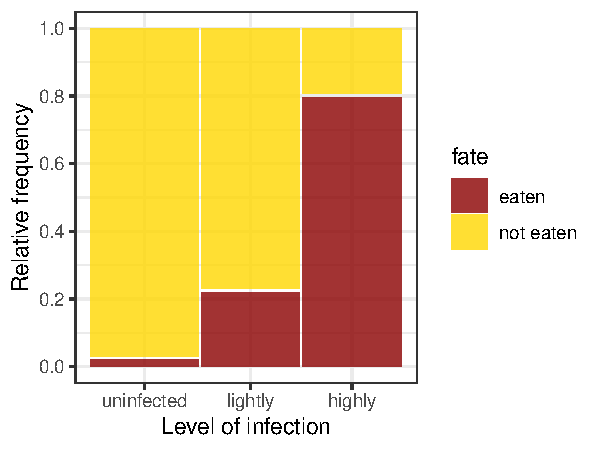
\includegraphics{BIOL202_files/figure-latex/unnamed-chunk-70-1.pdf}
\caption{\label{fig:unnamed-chunk-70}Relative frequency of cancer among women randomly assigned to control (n = 19942) and aspririn (n = 19934) treatment groups.}
\end{figure}

The mosaic plot shows that the incidence (or relative frequency) of cancer is almost identical in the treatment and control groups.

\textbf{IMPORTANT }
It is best practice to display the response variable as the ``fill'' variable in a mosaic plot.

\subsection{Conduct the Fisher's Exact Test}\label{do_fisher}

To do the Fisher's exact test on the cancer data, it is straightforward, using the \texttt{fisher.test} function from the \texttt{janitor} package.

There is also \texttt{fisher.test} function in the base R \texttt{stats} package, but it does not conform to \texttt{tidyverse} expectations. Hence our use of the \texttt{fisher.test} function from the \texttt{janitor} package. When there are multiple packages that use the same name for a function, we can specify the version we want by prefacing the function with the package name and two colons, like this: ``janitor::fisher.test()''

See the help file for the \texttt{janitor} version of the \texttt{fisher.test} function:

\begin{verbatim}
?janitor::fisher.test
\end{verbatim}

This function requires a two-way ``tabyl'' as the input, and we already know how to construct such a table.

We'll put the results in an object called ``cancer.fishertest'':

\begin{Shaded}
\begin{Highlighting}[]
\NormalTok{cancer.fishertest }\OtherTok{\textless{}{-}}\NormalTok{ cancer }\SpecialCharTok{\%\textgreater{}\%}
    \FunctionTok{tabyl}\NormalTok{(aspirinTreatment, response) }\SpecialCharTok{\%\textgreater{}\%}
\NormalTok{    janitor}\SpecialCharTok{::}\FunctionTok{fisher.test}\NormalTok{()}
\end{Highlighting}
\end{Shaded}

Let's look at the results:

\begin{Shaded}
\begin{Highlighting}[]
\NormalTok{cancer.fishertest}
\end{Highlighting}
\end{Shaded}

\begin{verbatim}
## 
##  Fisher's Exact Test for Count Data
## 
## data:  .
## p-value = 0.8311
## alternative hypothesis: true odds ratio is not equal to 1
## 95 percent confidence interval:
##  0.9342128 1.0892376
## sample estimates:
## odds ratio 
##   1.008744
\end{verbatim}

The \emph{P}-value associated with the test is 0.831, which is clearly greater than our \(\alpha\) of 0.05. We therefore FAIL to reject the null hypothesis.

You'll notice that the output includes the \textbf{odds ratio} and its 95\% confidence interval. The interval it provides is slightly different from the one we'll learn about below, but \textbf{when reporting the results of a Fisher's Exact test it is OK to report the confidence interval provided by the \texttt{fisher.test} function}. It is also OK to provide the slightly different one that we learn about below.

\textbf{Concluding statement}

\begin{quote}
There is no evidence that the probability of developing cancer differs between the control group and the aspirin treatment group (Fisher's Exact Test; \emph{P}-value = 0.831; odds ratio = 1.01; 95\% CI: 0.934 - 1.089).
\end{quote}

\textbf{TIP}
Report odds ratios to 2 decimal places, and associated measures of uncertainty to 3 decimal places

\section{Estimate the Odds of getting sick}\label{odds}

The \textbf{odds} of success (\emph{O}) are the probability of success (\emph{p}) divided by the probability of failure (1-\emph{p}):

\(O = \frac{p}{1-p}\)

Curiously, in health-related studies, a ``success'' is equated with getting ill!!

We'll use the data stored in the contingency table we produced before, called ``cancer.aspirin.table'':

\begin{Shaded}
\begin{Highlighting}[]
\NormalTok{cancer.aspirin.table }\OtherTok{\textless{}{-}}\NormalTok{ cancer }\SpecialCharTok{\%\textgreater{}\%}
  \FunctionTok{tabyl}\NormalTok{(aspirinTreatment, response) }\SpecialCharTok{\%\textgreater{}\%}
  \FunctionTok{adorn\_totals}\NormalTok{(}\AttributeTok{where =} \FunctionTok{c}\NormalTok{(}\StringTok{"row"}\NormalTok{, }\StringTok{"col"}\NormalTok{))}
\NormalTok{cancer.aspirin.table }
\end{Highlighting}
\end{Shaded}

\begin{verbatim}
##  aspirinTreatment Cancer No cancer Total
##           Aspirin   1438     18496 19934
##           Placebo   1427     18515 19942
##             Total   2865     37011 39876
\end{verbatim}

And recall that proportions are calculated using frequencies - which is exactly what we have in the table!

Thus, to estimate the ``odds'' of getting cancer while taking aspirin, we need to:

\begin{itemize}
\tightlist
\item
  first calculate the proportion (= probability) of women who got cancer while taking aspirin (= \({p}\))
\item
  then calculate the proportion (= probability) of women who remained healthy while taking aspirin (\(= 1-{p}\))
\item
  then calculate the odds as \(O = \frac{p}{1-p}\)
\end{itemize}

We'll do all of this in one go using a series of steps strung together with pipes (``\%\textgreater\%'').

Here's the code, and we'll explain each step after:

\begin{Shaded}
\begin{Highlighting}[]
\NormalTok{cancer.aspirin.table }\SpecialCharTok{\%\textgreater{}\%}
    \FunctionTok{filter}\NormalTok{(aspirinTreatment }\SpecialCharTok{==} \StringTok{"Aspirin"}\NormalTok{) }\SpecialCharTok{\%\textgreater{}\%}
    \FunctionTok{select}\NormalTok{(Cancer, Total) }\SpecialCharTok{\%\textgreater{}\%}
    \FunctionTok{mutate}\NormalTok{(}
       \AttributeTok{propCancer\_aspirin =}\NormalTok{ Cancer }\SpecialCharTok{/}\NormalTok{ Total,}
       \AttributeTok{propHealthy\_aspirin =} \DecValTok{1} \SpecialCharTok{{-}}\NormalTok{ propCancer\_aspirin,}
       \AttributeTok{oddsCancer\_aspirin =}\NormalTok{ propCancer\_aspirin}\SpecialCharTok{/}\NormalTok{propHealthy\_aspirin}
\NormalTok{    ) }
\end{Highlighting}
\end{Shaded}

\begin{verbatim}
##  Cancer Total propCancer_aspirin propHealthy_aspirin oddsCancer_aspirin
##    1438 19934         0.07213806           0.9278619         0.07774654
\end{verbatim}

\begin{itemize}
\tightlist
\item
  we first \texttt{filter} the table to return only the rows pertaining to the ``Aspirin'' treatment group; the frequencies that we need for the calculations are in this row
\item
  then we \texttt{select} the columns from that row with names ``Cancer'' and ``Total'', which include the frequency of women who got cancer while on Aspirin (under the ``Cancer'' column), and the total frequency of women in the Aspiring treatment group (in the ``Total'')
\item
  we then use the \texttt{mutate} function to create three new variables:

  \begin{itemize}
  \tightlist
  \item
    ``propCancer\_aspirin'' is calculated at the Cancer frequency divided by the Total frequency (within the Aspirin group)
  \item
    ``propHealth\_aspirin'' is calculated simply as 1 minus propCancer\_aspirin
  \item
    ``oddsCancer\_aspirin'' is calculated last as ``propCancer\_aspirin/propHealthy\_aspirin''
  \end{itemize}
\end{itemize}

Thus, the odds of getting cancer while on aspirin are about 0.08:1, or equivalently, approximately 1:13 (which you get from dividing 0.0777 into 1).

Alternatively, ``the odds are 13 to 1 that a women who took aspirin would \textbf{not} get cancer in the next 10 years''.

\begin{center}\rule{0.5\linewidth}{0.5pt}\end{center}

\begin{enumerate}
\def\labelenumi{\arabic{enumi}.}
\tightlist
\item
  Estimate odds
\end{enumerate}

\begin{itemize}
\tightlist
\item
  Estimate the odds that a woman in the placebo group would get cancer
\end{itemize}

\begin{center}\rule{0.5\linewidth}{0.5pt}\end{center}

\section{Estimate the odds ratio}\label{oddsratio}

We'll use the \texttt{oddsratio} function from the \texttt{epitools} package to calculate the odds ratio (\(\hat{OR}\)) and its 95\% confidence interval.

Check out the help file for the function:

\begin{verbatim}
?oddsratio
\end{verbatim}

The \texttt{oddsratio} function expects the contingency table to be arranged exactly like this:

\begin{verbatim}
#            treatment control
#  sick          a        b
#  healthy       c        d
\end{verbatim}

If you were calculating the odds ratio by hand, using the letters shown in the table above, the shortcut formula is:

\[\hat{OR} = \frac{{a/c}}{{b/d}}\]

Here's the code for producing the appropriately formatted 2 x 2 table as so:

\begin{Shaded}
\begin{Highlighting}[]
\NormalTok{cancer }\SpecialCharTok{\%\textgreater{}\%}
  \FunctionTok{tabyl}\NormalTok{(aspirinTreatment, response) }\SpecialCharTok{\%\textgreater{}\%}
    \FunctionTok{select}\NormalTok{(Cancer, }\StringTok{"No cancer"}\NormalTok{)}
\end{Highlighting}
\end{Shaded}

\begin{verbatim}
##  Cancer No cancer
##    1438     18496
##    1427     18515
\end{verbatim}

So thats what the \texttt{oddsratio} function is expecting as input.

However, it's also expecting it in the form of a ``matrix'' object.

Here's all the code at once, and we'll store the output (which comes in the form of a ``list'') in an object called ``cancer.odds'':

\begin{Shaded}
\begin{Highlighting}[]
\NormalTok{cancer.odds }\OtherTok{\textless{}{-}}\NormalTok{ cancer }\SpecialCharTok{\%\textgreater{}\%}
  \FunctionTok{tabyl}\NormalTok{(aspirinTreatment, response) }\SpecialCharTok{\%\textgreater{}\%}
    \FunctionTok{select}\NormalTok{(Cancer, }\StringTok{"No cancer"}\NormalTok{) }\SpecialCharTok{\%\textgreater{}\%}
    \FunctionTok{as.matrix}\NormalTok{() }\SpecialCharTok{\%\textgreater{}\%}
    \FunctionTok{oddsratio}\NormalTok{(}\AttributeTok{method =} \StringTok{"wald"}\NormalTok{)}
\end{Highlighting}
\end{Shaded}

We've seen the first two lines before. Then:

\begin{itemize}
\tightlist
\item
  we \texttt{select} the two columns associated with the ``Cancer'' and ``No cancer'' data. \textbf{NOTE} that because there's a space in the variable name ``No cancer'', we need to use quotation marks around it
\item
  Then we use the base \texttt{as.matrix} function to coerce the resulting 2 x 2 table that we've created into a matrix type object, which is what the \texttt{oddsratio} function is expecting.
\item
  lastly we run the \texttt{oddsratio} function, with the argument ``method = `wald'\,'' (don't worry about why)
\end{itemize}

Let's have a look at the rather verbose output:

\begin{Shaded}
\begin{Highlighting}[]
\NormalTok{cancer.odds}
\end{Highlighting}
\end{Shaded}

\begin{verbatim}
## $data
##       Cancer No cancer Total
## row1    1438     18496 19934
## row2    1427     18515 19942
## Total   2865     37011 39876
## 
## $measure
##                         NA
## odds ratio with 95% C.I. estimate     lower    upper
##                     [1,] 1.000000        NA       NA
##                     [2,] 1.008744 0.9349043 1.088415
## 
## $p.value
##          NA
## two-sided midp.exact fisher.exact chi.square
##      [1,]         NA           NA         NA
##      [2,]  0.8224348    0.8310911  0.8223986
## 
## $correction
## [1] FALSE
## 
## attr(,"method")
## [1] "Unconditional MLE & normal approximation (Wald) CI"
\end{verbatim}

This is more information than we need.

What we're interested in is the information under the ``\$measure'' part, and specifically the ``odds ratio with 95\% C.I.''.

To limit the output to the relevant information, use this code:

\begin{Shaded}
\begin{Highlighting}[]
\NormalTok{cancer.odds}\SpecialCharTok{$}\NormalTok{measure[}\DecValTok{2}\NormalTok{,]}
\end{Highlighting}
\end{Shaded}

\begin{verbatim}
##  estimate     lower     upper 
## 1.0087436 0.9349043 1.0884148
\end{verbatim}

This isolates the actual estimate of the odds ratio (\(\hat{OR}\)) with its 95\% confidence interval.

The estimate of the odds ratio is around 1.009, and notice the 95\% confidence interval encompasses one.

Given that the calculated 95\% confidence interval encompasses 1 (representing equal odds among treatment and control groups), there is presently no evidence that the odds of developing cancer differ among control and aspirin treatment groups.

\textbf{IMPORTANT }
The odds ratio and its 95\% confidence interval are useful to report in any analysis of a 2 x 2 contingency table that deals with health outcomes data like those used here.

\section{\texorpdfstring{\(\chi\)\textsuperscript{2} Contingency Test}{\textbackslash chi2 Contingency Test}}\label{chisquare}

When the contingency table is of dimensions greater than 2 x 2, the most commonly applied test is the \(\chi\)\textsuperscript{2} Contingency Test.

For this activity we're using the ``worm'' data associated with \textbf{Example 9.4 on page 244} of the test. Please read the example!

\begin{center}\rule{0.5\linewidth}{0.5pt}\end{center}

\subsection{Hypothesis statement}\label{chihyp}

As shown in the text example, we have a 2 x 3 contingency table, and we're testing for an association between two categorical variables.

Here are the null and alternative hypotheses (compare these to what's written in the text):

\textbf{H\textsubscript{0}}: There is no association between the level of trematode parasitism and the frequency (or probability) of being eaten.\\
\textbf{H\textsubscript{A}}: There is an association between the level of trematode parasitism and the frequency (or probability) of being eaten.

\begin{itemize}
\tightlist
\item
  We use \(\alpha\) = 0.05.\\
\item
  It is a two-tailed alternative hypothesis\\
\item
  We'll use a contingency test to test the null hypothesis, because this is appropriate for analyzing for association between two categorical variables, and when the resulting contingency table has dimension greater than 2 x 2.\\
\item
  We will use the \(\chi\)\textsuperscript{2} test statistic, with degrees of freedom equal to (r-1)(c-1), where ``r'' is the number of rows, and ``c'' is the number of colums, so (2-1)(3-1) = 2.\\
\item
  We must check assumptions of the \(\chi\)\textsuperscript{2} contingency test
\item
  It is always a good idea to present a figure to accompany your analysis; in the case of a contingency test, the figure heading will include information about the sample size / total number of observations
\end{itemize}

\begin{center}\rule{0.5\linewidth}{0.5pt}\end{center}

\subsection{Display the contingency table}\label{showwormcont}

Let's generate a contingency table:

\begin{Shaded}
\begin{Highlighting}[]
\NormalTok{worm }\SpecialCharTok{\%\textgreater{}\%}
  \FunctionTok{tabyl}\NormalTok{(fate, infection) }\SpecialCharTok{\%\textgreater{}\%}
  \FunctionTok{adorn\_totals}\NormalTok{(}\AttributeTok{where =} \FunctionTok{c}\NormalTok{(}\StringTok{"row"}\NormalTok{, }\StringTok{"col"}\NormalTok{))}
\end{Highlighting}
\end{Shaded}

\begin{verbatim}
##       fate highly lightly uninfected Total
##      eaten     37      10          1    48
##  not eaten      9      35         49    93
##      Total     46      45         50   141
\end{verbatim}

Hmm, the ordering of the categories of the categorical (factor) variable ``infection'' is the opposite to what is displayed in the text.

\textbf{TIP }
The ordering of the categories is not actually crucial to this type of analysis, but it's certainly better practice to show them in appropriate order!

In order to change the order of categories in a character variable, here's what you do (consult this \href{http://www.cookbook-r.com/Manipulating_data/Changing_the_order_of_levels_of_a_factor/}{resource} for additional info).

First, convert the character variable to a ``factor'' variable as follows:

\begin{Shaded}
\begin{Highlighting}[]
\NormalTok{worm}\SpecialCharTok{$}\NormalTok{infection }\OtherTok{\textless{}{-}} \FunctionTok{as.factor}\NormalTok{(worm}\SpecialCharTok{$}\NormalTok{infection)}
\end{Highlighting}
\end{Shaded}

Now check the default ordering of the levels using the \texttt{levels} function (it should be alphabetical):

\begin{Shaded}
\begin{Highlighting}[]
\FunctionTok{levels}\NormalTok{(worm}\SpecialCharTok{$}\NormalTok{infection)}
\end{Highlighting}
\end{Shaded}

\begin{verbatim}
## [1] "highly"     "lightly"    "uninfected"
\end{verbatim}

Now change the ordering as follows:

\begin{Shaded}
\begin{Highlighting}[]
\NormalTok{worm}\SpecialCharTok{$}\NormalTok{infection }\OtherTok{\textless{}{-}} \FunctionTok{factor}\NormalTok{(worm}\SpecialCharTok{$}\NormalTok{infection, }\AttributeTok{levels =} \FunctionTok{c}\NormalTok{(}\StringTok{"uninfected"}\NormalTok{, }\StringTok{"lightly"}\NormalTok{, }\StringTok{"highly"}\NormalTok{))}
\FunctionTok{levels}\NormalTok{(worm}\SpecialCharTok{$}\NormalTok{infection)}
\end{Highlighting}
\end{Shaded}

\begin{verbatim}
## [1] "uninfected" "lightly"    "highly"
\end{verbatim}

Now re-display the contingency table, first storing it in an object ``worm.table'':

\begin{Shaded}
\begin{Highlighting}[]
\NormalTok{worm.table }\OtherTok{\textless{}{-}}\NormalTok{ worm }\SpecialCharTok{\%\textgreater{}\%}
  \FunctionTok{tabyl}\NormalTok{(fate, infection) }\SpecialCharTok{\%\textgreater{}\%}
  \FunctionTok{adorn\_totals}\NormalTok{(}\AttributeTok{where =} \FunctionTok{c}\NormalTok{(}\StringTok{"row"}\NormalTok{, }\StringTok{"col"}\NormalTok{))}
\NormalTok{worm.table}
\end{Highlighting}
\end{Shaded}

\begin{verbatim}
##       fate uninfected lightly highly Total
##      eaten          1      10     37    48
##  not eaten         49      35      9    93
##      Total         50      45     46   141
\end{verbatim}

That's better!

Visualize it nicely with \texttt{kable}:

\begin{Shaded}
\begin{Highlighting}[]
\FunctionTok{kable}\NormalTok{(worm.table)}
\end{Highlighting}
\end{Shaded}

fate

uninfected

lightly

highly

Total

eaten

1

10

37

48

not eaten

49

35

9

93

Total

50

45

46

141

\subsection{Visualize a mosaic plot}\label{mosaicworm}

Here's a mosaic plot with an ideal figure caption included:

\begin{Shaded}
\begin{Highlighting}[]
\NormalTok{worm }\SpecialCharTok{\%\textgreater{}\%}
    \FunctionTok{ggplot}\NormalTok{() }\SpecialCharTok{+}
    \FunctionTok{geom\_mosaic}\NormalTok{(}\FunctionTok{aes}\NormalTok{(}\AttributeTok{x =} \FunctionTok{product}\NormalTok{(infection), }\AttributeTok{fill =}\NormalTok{ fate)) }\SpecialCharTok{+}
    \FunctionTok{scale\_fill\_manual}\NormalTok{(}\AttributeTok{values=}\FunctionTok{c}\NormalTok{(}\StringTok{"darkred"}\NormalTok{, }\StringTok{"gold"}\NormalTok{)) }\SpecialCharTok{+}
    \FunctionTok{scale\_y\_continuous}\NormalTok{(}\AttributeTok{breaks =} \FunctionTok{seq}\NormalTok{(}\DecValTok{0}\NormalTok{, }\DecValTok{1}\NormalTok{, }\AttributeTok{by =} \FloatTok{0.2}\NormalTok{)) }\SpecialCharTok{+}
    \FunctionTok{xlab}\NormalTok{(}\StringTok{"Level of infection"}\NormalTok{) }\SpecialCharTok{+}
    \FunctionTok{ylab}\NormalTok{(}\StringTok{"Relative frequency"}\NormalTok{) }\SpecialCharTok{+}
    \FunctionTok{theme\_bw}\NormalTok{()}
\end{Highlighting}
\end{Shaded}

\begin{figure}
\centering
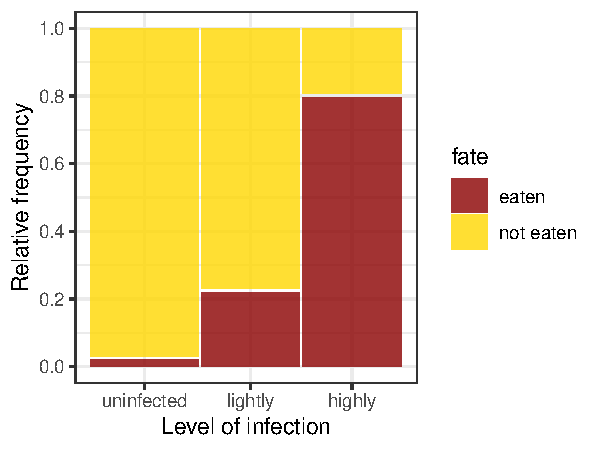
\includegraphics{BIOL202_files/figure-latex/unnamed-chunk-75-1.pdf}
\caption{\label{fig:unnamed-chunk-75}Mosaic plot of bird predation on killifish having different levels of trematode parasitism. A total of 50, 45, and 46 fish were in the uninfected, lightly infected, and highly infected groups.}
\end{figure}

In the code above we manually specified the two fill colours using the \texttt{scale\_fill\_manual} function.

\subsection{Check the assumptions}\label{checkchiassum}

The \(\chi\)\textsuperscript{2} contingency test (also known as association test) has assumptions that \textbf{must be checked} prior to proceeding:

\begin{itemize}
\tightlist
\item
  none of the categories should have an expected frequency of less than one
\item
  no more than 20\% of the categories should have expected frequencies less than five
\end{itemize}

To test these assumptions, we need to actually conduct the test, because in doing so R calculates the \textbf{expected frequencies} for us.

Conduct the test using the \texttt{chisq.test} function from \texttt{janitor} package. \textbf{NOTE} this again overlaps with a function name from the base R package, so we'll need to specify that we want the ``janitor'' version of the function.

We need our contingency table as input to the function, but this time without margin totals.

We'll assign the results to an object ``worm.chisq.results'':

\begin{Shaded}
\begin{Highlighting}[]
\NormalTok{worm.chisq.results }\OtherTok{\textless{}{-}}\NormalTok{ worm }\SpecialCharTok{\%\textgreater{}\%}
    \FunctionTok{tabyl}\NormalTok{(fate, infection) }\SpecialCharTok{\%\textgreater{}\%}
\NormalTok{    janitor}\SpecialCharTok{::}\FunctionTok{chisq.test}\NormalTok{()}
\end{Highlighting}
\end{Shaded}

Have a look at the output:

\begin{Shaded}
\begin{Highlighting}[]
\NormalTok{worm.chisq.results}
\end{Highlighting}
\end{Shaded}

\begin{verbatim}
## 
##  Pearson's Chi-squared test
## 
## data:  .
## X-squared = 69.756, df = 2, p-value = 7.124e-16
\end{verbatim}

Although only a few bits of information are provided here, the object actually contains a lot more information.

Don't try getting an overview of the object using our usual \texttt{skim\_without\_charts} approach.. that won't work.

Instead, simply use this code:

\begin{Shaded}
\begin{Highlighting}[]
\FunctionTok{names}\NormalTok{(worm.chisq.results)}
\end{Highlighting}
\end{Shaded}

\begin{verbatim}
## [1] "statistic" "parameter" "p.value"   "method"    "data.name" "observed" 
## [7] "expected"  "residuals" "stdres"
\end{verbatim}

As you can see, one of the names is \texttt{expected}. This is what holds our expected frequencies (and note that these values do not need to be whole numbers, unlike the observed frequencies):

\begin{Shaded}
\begin{Highlighting}[]
\FunctionTok{kable}\NormalTok{(worm.chisq.results}\SpecialCharTok{$}\NormalTok{expected)}
\end{Highlighting}
\end{Shaded}

fate

uninfected

lightly

highly

eaten

eaten

17.02128

15.31915

15.65957

not eaten

not eaten

32.97872

29.68085

30.34043

We see that all our assumptions are met: none of the cells (cross-classified categories) in the table have an expected frequency of less than one, and no more than 20\% of the cells have expected frequencies less than five.

\subsection{Get the results of the test}\label{chiresults}

We can see the results of the \(\chi\)\textsuperscript{2} test by simply typing the name of the results object:

\begin{Shaded}
\begin{Highlighting}[]
\NormalTok{worm.chisq.results}
\end{Highlighting}
\end{Shaded}

\begin{verbatim}
## 
##  Pearson's Chi-squared test
## 
## data:  .
## X-squared = 69.756, df = 2, p-value = 7.124e-16
\end{verbatim}

This shows a very large value of \(\chi\)\textsuperscript{2} (69.76) and a very small \emph{P}-value - much smaller than our stated \(\alpha\). So we reject the null hypothesis.

\textbf{Concluding statement}

\begin{quote}
The probability of being eaten is significantly associated with the level of trematode parasitism (\(\chi\)\textsuperscript{2} contingency test; \emph{df} = 2; \(\chi\)\textsuperscript{2} = 69.76; \emph{P} \textless{} 0.001). Based on our mosaic plot (Fig. X), the probability of being eaten increases substantially with increasing intensity of parasitism.
\end{quote}

\chapter{Analyzing a single numerical variable}\label{single_numeric}

\textbf{Tutorial learning objectives}

\begin{itemize}
\tightlist
\item
  Learn about the one-sample \emph{t}-test, which compares the mean from a sample of individuals to a value for the population mean (\(\mu_0\)) proposed in the null hypothesis
\item
  Learn the assumptions of a one-sample \emph{t}-test
\item
  Learn how to calculate an exact confidence interval for a population mean (\(\mu\))
\item
  Learn the confidence interval approach for testing the plausibility of a hypothesized value for \(\mu\)
\end{itemize}

\begin{center}\rule{0.5\linewidth}{0.5pt}\end{center}

\section{Load packages and import data}\label{singlenum_packages_data}

Load the \texttt{tidyverse}, \texttt{knitr}, \texttt{naniar}, and \texttt{janitor} packages:

\begin{Shaded}
\begin{Highlighting}[]
\FunctionTok{library}\NormalTok{(tidyverse)}
\FunctionTok{library}\NormalTok{(knitr)}
\FunctionTok{library}\NormalTok{(naniar)}
\FunctionTok{library}\NormalTok{(janitor)}
\end{Highlighting}
\end{Shaded}

We'll use the following datasets:

\begin{itemize}
\tightlist
\item
  the ``bodytemp'' dataset. These are the data associated with Example 11.3 in the text (page 310)
\item
  the ``stalkies'' dataset. These are the data associated with Example 11.2 in the text (page 307)
\end{itemize}

\begin{Shaded}
\begin{Highlighting}[]
\NormalTok{bodytemp }\OtherTok{\textless{}{-}} \FunctionTok{read\_csv}\NormalTok{(}\StringTok{"https://raw.githubusercontent.com/ubco{-}biology/BIOL202/main/data/bodytemp.csv"}\NormalTok{)}
\NormalTok{stalkies }\OtherTok{\textless{}{-}} \FunctionTok{read\_csv}\NormalTok{(}\StringTok{"https://raw.githubusercontent.com/ubco{-}biology/BIOL202/main/data/stalkies.csv"}\NormalTok{)}
\end{Highlighting}
\end{Shaded}

\textbf{Reminder: }
Before proceeding further, remember to get an overview of each of these datasets.

\begin{center}\rule{0.5\linewidth}{0.5pt}\end{center}

\section{\texorpdfstring{One-sample \emph{t}-test}{One-sample t-test}}\label{onesamp_t_test}

We previously learned statistical tests for testing hypotheses about categorical response variables. For instance, we learned how to conduct a \(\chi^2\) \hyperref[chisquare]{contingency test} to test the null hypothesis that there is no association between two categorical variables.

Here we are going to learn our first statistical test for testing hypotheses about a numeric response variable, specifically one whose probability distribution in the population is normally distributed.

\begin{center}\rule{0.5\linewidth}{0.5pt}\end{center}

\subsection{Hypothesis statement}\label{onesamp_hyp}

Review the earlier tutorial that lists the \hyperref[hyp_steps]{steps to hypothesis testing}.

We'll use the body temperature data for this example, as described in example 11.3 in the text.

Americans are taught as kids that the normal human body temperature is 98.6 degrees Farenheit.

Are the data consistent with this assertion?

\begin{itemize}
\tightlist
\item
  We'll use a one-sample \emph{t}-test test to test the null hypothesis, because we're dealing with a single numerical response variable, and we're using a sample of individuals to draw inferences about a hypothesized (population) mean \(\mu_0\)
\end{itemize}

The hypotheses for this test:

\textbf{H\textsubscript{0}}: The mean human body temperature is 98.6\(^\circ\)F (\(\mu_0\) = 98.6\(^\circ\)F).\\
\textbf{H\textsubscript{A}}: The mean human body temperature is not 98.6\(^\circ\)F (\(\mu_0 \ne 98.6^\circ\)F).

\textbf{TIP }
You can add a degree symbol using this syntax in markdown: \texttt{\$\^{}\textbackslash{}circ\$}, so degrees Celsius would be \texttt{\$\^{}\textbackslash{}circ\$C}

\begin{itemize}
\tightlist
\item
  We'll use an \(\alpha\) level of 0.05.\\
\item
  It is a two-tailed alternative hypothesis
\end{itemize}

\begin{center}\rule{0.5\linewidth}{0.5pt}\end{center}

\subsection{\texorpdfstring{Assumptions of one-sample \emph{t}-test}{Assumptions of one-sample t-test}}\label{onesamp_assumptions}

The \textbf{assumptions} of the one-sample \emph{t}-test are as follows:

\begin{itemize}
\tightlist
\item
  the sampling units are randomly sampled from the population (a standard assumption)
\item
  the variable is normally distributed in the population
\end{itemize}

Consult the \href{https://ubco-biology.github.io/BIOL202/checking-assumptions-and-data-transformations.html}{``checking assumptions'' tutorial} for how to formally check the second assumption. For now we'll assume both assumptions are met.

If the normal distribution assumption is not met, and no \href{https://ubco-biology.github.io/BIOL202/checking-assumptions-and-data-transformations.html}{data transformation} helps, then one can conduct a ``non-parametric'' test in lieu of the one-sample \emph{t}-test, including a ``Sign test'' or a ``Wilcoxon signed-rank test''. A tutorial on non-parametric tests is under development, but will not be deployed until 2023. Consult chapter 13 in the Whitlock \& Schluter text, and this \href{https://whitlockschluter3e.zoology.ubc.ca/RExamples/Rcode_Chapter_13.html\#new_methods_on_this_page}{website} for some R examples.

\begin{center}\rule{0.5\linewidth}{0.5pt}\end{center}

\subsection{\texorpdfstring{A graph to accompany a one-sample \emph{t}-test}{A graph to accompany a one-sample t-test}}\label{onesamp_graph}

Let's create a histogram of the body temperatures, because this is the most appropriate way to visualize the frequency distribution of a single numeric variable.

Histograms may look a little wonky if you have small sample sizes. This is OK!

If you forget how to create a histogram, consult the previous tutorial on \hyperref[vis_histogram]{visualizing a single numeric variable}.

Here we'll learn a few more tricks for producing a high-quality histogram.

The first step is to figure out the minimum and maximum values of your numeric variable, and you should have already done this when using the \texttt{skim\_without\_charts} function to get an overview of the dataset (when you first imported the data).

For the \texttt{temperature} variable, our minimum and maximum values were 97.4 and 100, respectively.

We'll use this information to ensure that the histogram spans the appropriate range along the x-axis, and to decide on the appropriate ``bin widths'':

\begin{Shaded}
\begin{Highlighting}[]
\NormalTok{bodytemp }\SpecialCharTok{\%\textgreater{}\%} 
  \FunctionTok{ggplot}\NormalTok{(}\FunctionTok{aes}\NormalTok{(}\AttributeTok{x =}\NormalTok{ temperature)) }\SpecialCharTok{+}
  \FunctionTok{geom\_histogram}\NormalTok{(}\AttributeTok{binwidth =} \FloatTok{0.5}\NormalTok{, }\AttributeTok{boundary =} \DecValTok{97}\NormalTok{, }
                 \AttributeTok{color =} \StringTok{"black"}\NormalTok{, }\AttributeTok{fill =} \StringTok{"lightgrey"}\NormalTok{,) }\SpecialCharTok{+}
  \FunctionTok{xlab}\NormalTok{(}\StringTok{"Body temperature (degrees F)"}\NormalTok{) }\SpecialCharTok{+}
  \FunctionTok{ylab}\NormalTok{(}\StringTok{"Frequency"}\NormalTok{) }\SpecialCharTok{+}
  \FunctionTok{theme\_bw}\NormalTok{()}
\end{Highlighting}
\end{Shaded}

\begin{figure}
\centering
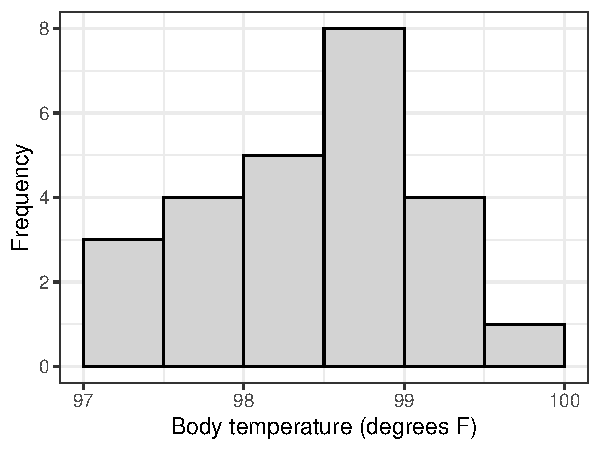
\includegraphics{BIOL202_files/figure-latex/unnamed-chunk-78-1.pdf}
\caption{\label{fig:unnamed-chunk-78}Frequency distribution of body temperature (degrees Farenheit) for 25 randomly chosen healthy people.}
\end{figure}

Notice the new argument to the \texttt{geom\_histogram} function: ``boundary''. Why include this? The minimum value in our dataset is 97.4. Based on our overview of the data, we decided to use a ``binwidth'' of 0.5. Therefore, it made most sense to have our bins (bars) start at 97, the first whole number preceding our minimum value, then have breaks every 0.5 units thereafter. Constructing the histogram this way makes it easier to interpret.

Recall that it can take a few times playing with different values of ``binwidth'' to make the histogram have the right number of bins.

\textbf{Interpreting the histogram}:

\begin{quote}
We can see in the histogram above that most of the individuals had temperatures between 98 and 99\(^\circ\)F, which is consistent with conventional wisdom, but there are 7 people with temperature below 98\(^\circ\)F, and 5 with temperatures above 99\(^\circ\)F. The frequency distribution is unimodal but not especially symmetrical.
\end{quote}

\begin{center}\rule{0.5\linewidth}{0.5pt}\end{center}

\subsection{\texorpdfstring{Conduct the one-sample \emph{t}-test}{Conduct the one-sample t-test}}\label{onesamp_test}

We use the \texttt{t.test} function (it comes with the \texttt{base} package loaded with R) to conduct a one-sample \emph{t}-test.

\begin{verbatim}
?t.test  
\end{verbatim}

This function is used for both one-sample and two-sample \emph{t}-tests (covered later), and for calculating 95\% confidence intervals for a mean (later in this tutorial).

Because this function has multiple purposes, be sure to pay attention to the arguments.

Here's the code, which we'll explain after:

\begin{Shaded}
\begin{Highlighting}[]
\NormalTok{body.ttest }\OtherTok{\textless{}{-}}\NormalTok{ bodytemp }\SpecialCharTok{\%\textgreater{}\%}
  \FunctionTok{select}\NormalTok{(temperature) }\SpecialCharTok{\%\textgreater{}\%}
\FunctionTok{t.test}\NormalTok{(}\AttributeTok{mu =} \FloatTok{98.6}\NormalTok{, }\AttributeTok{alternative =} \StringTok{"two.sided"}\NormalTok{, }\AttributeTok{conf.level =} \FloatTok{0.95}\NormalTok{) }
\end{Highlighting}
\end{Shaded}

\begin{itemize}
\tightlist
\item
  We first assign our results to a new object called ``body.ttest''
\item
  We then \texttt{select} the variable ``temperature'', as this is the one being analyzed
\item
  We then conduct the test using the function \texttt{t.test}, specifying the null hypothesized value as ``mu = 98.6''
\item
  We specify ``two.sided'' for the ``alternative'' argument
\item
  We provide the ``conf.level'' of 0.95, which is equal to \(1-\alpha\)
\end{itemize}

Let's look at the results:

\begin{Shaded}
\begin{Highlighting}[]
\NormalTok{body.ttest}
\end{Highlighting}
\end{Shaded}

\begin{verbatim}
## 
##  One Sample t-test
## 
## data:  .
## t = -0.56065, df = 24, p-value = 0.5802
## alternative hypothesis: true mean is not equal to 98.6
## 95 percent confidence interval:
##  98.24422 98.80378
## sample estimates:
## mean of x 
##    98.524
\end{verbatim}

The output includes:

\begin{itemize}
\tightlist
\item
  The calculated test statistic \emph{t}
\item
  The degrees of freedom
\item
  The \emph{P}-value for the test
\item
  A 95\% confidence interval for \(\mu\)
\item
  The sample-based estimate, denoted ``mean of x'', but is our (\(\bar{Y}\))
\end{itemize}

The observed \emph{P}-value for our test is larger than our \(\alpha\) level of 0.05. We therefore fail to reject the null hypothesis.

\begin{center}\rule{0.5\linewidth}{0.5pt}\end{center}

\subsection{\texorpdfstring{Concluding statement for the one-sample \emph{t}-test}{Concluding statement for the one-sample t-test}}\label{onesamp_conclude}

Here's an example of an appropriately worded concluding statement, including all the relevant information:

\begin{quote}
We have no reason to reject the null hypothesis that the mean body temperature of a healthy human is 98.6\(^\circ\)F (one-sample \emph{t}-test; \emph{t} = -0.56; \emph{n} = 25 or \emph{df} = 24; \emph{P} = 0.58; 95\% confidence interval: 98.244 \(< \mu <\) 98.804).
\end{quote}

\textbf{TIP }
The confidence interval provided by the \texttt{t.test} function is accurate and good to report with your concluding statement for a one-sample \emph{t}-test. However, below we learn a different way to calculate the confidence interval.

\begin{center}\rule{0.5\linewidth}{0.5pt}\end{center}

\section{\texorpdfstring{Confidence intervals for \(\mu\)}{Confidence intervals for \textbackslash mu}}\label{t_confidence}

In an earlier \hyperref[confint_rough]{tutorial} we learned about the \textbf{rule of thumb 95\% confidence interval}.

Now we will learn how to calculate confidence intervals more precisely.

There are two typical uses of confidence intervals:

\begin{itemize}
\tightlist
\item
  When we are \emph{estimating} a population parameter (such as \(\mu\)) based on a random sample, in which case the confidence interval is an ideal measure of precision to accompany our estimate
\item
  As an alternative to a formal hypothesis test, in which case we determine whether the hypothesized value of the population parameter (e.g.~\(\mu_0\)) is a plausible value for \(\mu\), based on the confidence interval calculated using our sample data
\end{itemize}

We'll explore the latter use of confidence intervals later in this tutorial. For now, let's demonstrate the first use of confidence intervals: as a measure of precision for an estimate.

\begin{center}\rule{0.5\linewidth}{0.5pt}\end{center}

\subsection{Confidence interval as a measure of precision for an estimate}\label{conf_precision}

A straightforward way to calculate the confidence interval for the mean of a numeric variable is using the \texttt{t.test} function. For an example, see this \hyperref[onesamp_test]{tutorial section}.

The formula for a 95\% confidence interval for \(\mu\) is:

\[\bar{Y} - t_{0.05(2),df}SE_{\bar{Y}} < \mu <  \bar{Y} + t_{0.05(2),df}SE_{\bar{Y}}\]

The \(t_{0.05(2),df}\) represents the critical value of \emph{t} for a two-tailed test with \(\alpha = 0.05\), and \emph{degrees of freedom} (df), which is calculated from our sample size as \(df = n - 1\).

\(SE_{\bar{Y}}\) is the familiar \hyperref[sem_page]{standard error of the mean}, calculated as:

\[SE_\bar{Y} = \frac{s}{\sqrt{n}}\]

The lower 95 confidence limit is the value to the left of the \(\mu\) in the equation above, and the upper 95\% confidence limit is the value to the right of of the \(\mu\) in the equation.

So now we need to figure out the critical value \(t_{0.05(2),df}\).

For the body temperature example, we have \(n = 25\) and thus \(df = 25-1 = 24\).

Optionally, we could assign all these values to objects first, for use later:

\begin{Shaded}
\begin{Highlighting}[]
\NormalTok{alpha }\OtherTok{\textless{}{-}} \FloatTok{0.05}
\NormalTok{n }\OtherTok{\textless{}{-}} \DecValTok{25}
\NormalTok{d\_f }\OtherTok{=}\NormalTok{ n }\SpecialCharTok{{-}} \DecValTok{1}
\end{Highlighting}
\end{Shaded}

The function we use to find the critical value of \emph{t} is the base function \texttt{qt}:

\begin{verbatim}
?qt
\end{verbatim}

The \texttt{qt} function only deals with one tail of the distribution. Thus, if we have a two-sided alternative hypothesis, we need to divide our \(\alpha\) level by two in order to calculate the appropriate critical value of \emph{t}.

The following graph illustrates this for the \emph{t} distribution associated with \emph{df} = 24 and \(\alpha(2)\) = 0.05. Specifically, the \(t_{crit}\) values are shown by the vertical lines, and delimit the points beyond which the area under the curve towards the tail is equal to \(\alpha / 2\) (and thus the total area of both red zones= \(\alpha\)).

\begin{figure}
\centering
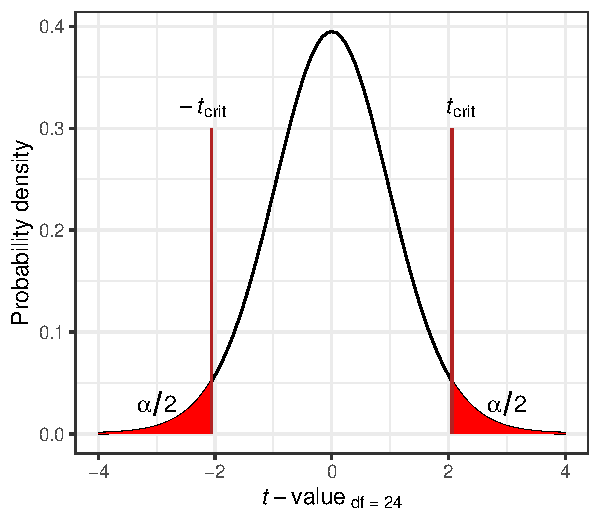
\includegraphics{BIOL202_files/figure-latex/unnamed-chunk-80-1.pdf}
\caption{\label{fig:unnamed-chunk-80}The \emph{t} distribution for df = 24.}
\end{figure}

Here's the code to calculate the critical value of \emph{t}, and recall that we've defined \texttt{alpha} and \texttt{d\_f} above:

\begin{Shaded}
\begin{Highlighting}[]
\NormalTok{tcrit }\OtherTok{\textless{}{-}} \FunctionTok{qt}\NormalTok{(}\AttributeTok{p =}\NormalTok{ alpha}\SpecialCharTok{/}\DecValTok{2}\NormalTok{, }\AttributeTok{df =}\NormalTok{ d\_f, }\AttributeTok{lower.tail =} \ConstantTok{FALSE}\NormalTok{)}
\end{Highlighting}
\end{Shaded}

In the code above:

\begin{itemize}
\tightlist
\item
  We assign the result to a new object called \texttt{tcrit}
\item
  The \(\alpha(2) = 0.05\) is \textbf{divided by 2}, because we have a two-sided alternative hypothesis
\item
  The degrees of freedom (which we stored in an object called \texttt{d\_f})
\item
  We specified \texttt{lower.tail\ =\ FALSE} to tell R that we'd like to focus on calculating the critical value for the right-hand (upper) tail, and thus the positive critical value
\end{itemize}

Alternatively, we could simply provide the values of alpha and degrees of freedom directly to the function arguments:

\begin{Shaded}
\begin{Highlighting}[]
\NormalTok{tcrit }\OtherTok{\textless{}{-}} \FunctionTok{qt}\NormalTok{(}\FloatTok{0.05}\SpecialCharTok{/}\DecValTok{2}\NormalTok{, }\AttributeTok{df =} \DecValTok{24}\NormalTok{, }\AttributeTok{lower.tail =} \ConstantTok{FALSE}\NormalTok{)}
\end{Highlighting}
\end{Shaded}

\textbf{TIP }
If instead we wanted to calculate a 99\% confidence interval, then \(\alpha(2) = 0.01\), and we'd use 0.01 instead of 0.05 in the \texttt{qt} function above. Try it out!

Now let's see what the output is:

\begin{Shaded}
\begin{Highlighting}[]
\NormalTok{tcrit}
\end{Highlighting}
\end{Shaded}

\begin{verbatim}
## [1] 2.063899
\end{verbatim}

So to recap, this procedure used R code to give us what we'd otherwise need to look up in a statistical table, like the one provided in the text book.

Now that we've determined the value for \(t_{0.05(2),24}\), we need to calculate \(SE_{\bar{Y}}\), which we \hyperref[sem_page]{already learned how to do}.
So let's improve on what we learned in the estimation tutorial, where we learned how to calculate the \hyperref[confint_rough]{rule-of-thumb confidence interval}.

There, we generated a table (actually a ``tibble'') of summary statistics that included the rule-of-thumb confidence limits; now we can include the precisely calculated lower and upper 95\% confidence limits.

Recall that we've already created an object ``tcrit'' that holds our required critical value of \emph{t}.

Here we'll assign the output to a tibble called ``bodytemp.stats'':

\begin{Shaded}
\begin{Highlighting}[]
\NormalTok{bodytemp.stats }\OtherTok{\textless{}{-}}\NormalTok{ bodytemp }\SpecialCharTok{\%\textgreater{}\%}
  \FunctionTok{summarise}\NormalTok{(}
    \AttributeTok{Count =} \FunctionTok{n}\NormalTok{() }\SpecialCharTok{{-}}\NormalTok{ naniar}\SpecialCharTok{::}\FunctionTok{n\_miss}\NormalTok{(temperature),}
    \AttributeTok{Mean\_temp =} \FunctionTok{mean}\NormalTok{(temperature, }\AttributeTok{na.rm =} \ConstantTok{TRUE}\NormalTok{),}
    \AttributeTok{SD\_temp =} \FunctionTok{sd}\NormalTok{(temperature, }\AttributeTok{na.rm =} \ConstantTok{TRUE}\NormalTok{),}
    \AttributeTok{SEM =}\NormalTok{ SD\_temp}\SpecialCharTok{/}\FunctionTok{sqrt}\NormalTok{(Count),}
    \AttributeTok{Lower\_95\_CL =}\NormalTok{ Mean\_temp }\SpecialCharTok{{-}}\NormalTok{ tcrit }\SpecialCharTok{*}\NormalTok{ SEM,}
    \AttributeTok{Upper\_95\_CL =}\NormalTok{ Mean\_temp }\SpecialCharTok{+}\NormalTok{ tcrit }\SpecialCharTok{*}\NormalTok{ SEM}
\NormalTok{  )}
\end{Highlighting}
\end{Shaded}

The \texttt{summarise} function is used to create new summary variables, as we've learned before.

The new part here is that we're calculating precisely the lower and upper 95\% confidence limits, using the combination of the \texttt{tcrit} value that we calculated and the ``SEM'' (standard error).

Now let's use the \texttt{kable} function to produce a nice table, and here we'll use ``digits = 3'' because that's appropriate for the confidence limits (noting that it will report three decimal places for all our calculated values):

\begin{Shaded}
\begin{Highlighting}[]
\FunctionTok{kable}\NormalTok{(bodytemp.stats, }\AttributeTok{digits =} \DecValTok{3}\NormalTok{)}
\end{Highlighting}
\end{Shaded}

Count

Mean\_temp

SD\_temp

SEM

Lower\_95\_CL

Upper\_95\_CL

25

98.524

0.678

0.136

98.244

98.804

If we wanted to report the confidence interval on its own, we can get the necessary information from our newly created tibble ``bodytemp.stats'', and type the following inline code in our markdown text (NOT in a code chunk):

\begin{figure}
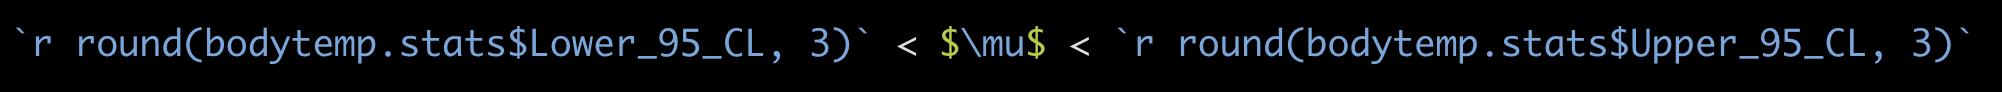
\includegraphics[width=27.81in]{./more/confint_inline_code} \caption{Example of inline markdown and R code for a confidence interval}\label{fig:unnamed-chunk-81}
\end{figure}

Which will provide:

98.244 \textless{} \(\mu\) \textless{} 98.804

\subsection{Confidence interval approach to hypothesis testing}\label{conf_hyp}

Recall our null and alternative hypotheses for the body temperature example:

\textbf{H\textsubscript{0}}: The mean human body temperature is 98.6\(^\circ\)F (\(\mu_0\) = 98.6\(^\circ\)F).\\
\textbf{H\textsubscript{A}}: The mean human body temperature is not 98.6\(^\circ\)F (\(\mu_0 \ne 98.6^\circ\)F).

The null hypothesis proposed \(\mu_0\) = 98.6\(^\circ\)F.

The confidence interval approach to testing a null hypothesis involves:

\begin{itemize}
\tightlist
\item
  specifying a level of confidence, 100\% \(\times\) (1-\(\alpha\)), such as 95\%
\item
  calculating the confidence interval for \(\mu\) using the sample data
\item
  determining whether or not \(\mu_0\) lies within the calculated confidence interval
\end{itemize}

If it does, then the proposed value of \(\mu_0\) is plausible, and there's no reason to reject the null hypothesis.

If it does not, then we reject the null hypothesis and conclude that plausible values of \(\mu\) are between our lower and upper confidence limits.

For example, for the body temperature example, we calculated a 95\% confidence interval as:

98.244 \textless{} \(\mu\) \textless{} 98.804

The hypothesized value of \(\mu_0\) was 98.6\(^\circ\)F, which is encompassed by our confidence interval. Thus, it is a plausible value, and there is no reason to reject the null hypothesis.

\begin{center}\rule{0.5\linewidth}{0.5pt}\end{center}

\begin{enumerate}
\def\labelenumi{\arabic{enumi}.}
\tightlist
\item
  Practice confidence intervals
\end{enumerate}

\begin{itemize}
\tightlist
\item
  First, using the \texttt{bodytemp} dataset, calculate the 99\% confidence interval for the mean body temperature in the population.\\
\item
  Then, using the ``stalkies'' dataset, use the confidence interval approach (95\% confidence) to test the hypothesis that the average eye span in the population is \(\mu_0\) = 8.1mm
\end{itemize}

\begin{center}\rule{0.5\linewidth}{0.5pt}\end{center}

\chapter{Comparing means among two groups}\label{compare_two_means}

\textbf{Tutorial learning objectives}

\begin{itemize}
\tightlist
\item
  Learn about paired and two-sample study designs for comparing the mean of a numeric response variable among two categories of a categorical variable (i.e.~two groups)
\item
  Learn about the paired \emph{t}-test for testing a hypothesis about the difference between means in a paired design (\(d\))
\item
  Learn about the two-sample \emph{t}-test for testing a hypothesis about the difference between two population means (\(\mu_1 - \mu_2\))
\item
  Learn the assumptions of the paired and two-sample \emph{t}-tests
\item
  Learn how to calculate an exact confidence interval for the difference between two means
\item
  Learn the confidence interval approach for testing the plausibility of a hypothesized value for \(\mu_1 - \mu_2\)
\end{itemize}

\section{Load packages and import data}\label{twomean_packages_data}

Load the \texttt{tidyverse}, \texttt{knitr}, \texttt{naniar}, \texttt{car}, \texttt{skimr}, and \texttt{janitor} packages:

\begin{Shaded}
\begin{Highlighting}[]
\FunctionTok{library}\NormalTok{(tidyverse)}
\FunctionTok{library}\NormalTok{(knitr)}
\FunctionTok{library}\NormalTok{(naniar)}
\FunctionTok{library}\NormalTok{(janitor)}
\FunctionTok{library}\NormalTok{(skimr)}
\FunctionTok{library}\NormalTok{(car)}
\end{Highlighting}
\end{Shaded}

And we also need the \texttt{broom} package, which may be new to you.

\begin{Shaded}
\begin{Highlighting}[]
\FunctionTok{library}\NormalTok{(broom)}
\end{Highlighting}
\end{Shaded}

The following datasets are required:

\begin{itemize}
\tightlist
\item
  the ``blackbird'' dataset. These are the data associated with Example 12.2 in the text (page 330)
\item
  the ``students'' dataset, describing characteristics of students from BIOL202 from several years back
\end{itemize}

\begin{Shaded}
\begin{Highlighting}[]
\NormalTok{blackbird }\OtherTok{\textless{}{-}} \FunctionTok{read\_csv}\NormalTok{(}\StringTok{"https://raw.githubusercontent.com/ubco{-}biology/BIOL202/main/data/blackbird.csv"}\NormalTok{, }\AttributeTok{show\_col\_types =} \ConstantTok{FALSE}\NormalTok{)}
\NormalTok{students }\OtherTok{\textless{}{-}} \FunctionTok{read\_csv}\NormalTok{(}\StringTok{"https://raw.githubusercontent.com/ubco{-}biology/BIOL202/main/data/students.csv"}\NormalTok{, }\AttributeTok{show\_col\_types =} \ConstantTok{FALSE}\NormalTok{)}
\end{Highlighting}
\end{Shaded}

\section{\texorpdfstring{Paired \emph{t}-test}{Paired t-test}}\label{paired-t-test}

We'll use the \texttt{blackbird} dataset for this example.

For 13 red-winged blackbirds, measurements of antibodies were taken before and after implantation with testosterone. Thus, the same bird was measured twice. Clearly, these measurements are not independent, hence the need for a ``paired'' \emph{t}-test.

Let's first have a look at the \texttt{blackbird} dataset:

\begin{Shaded}
\begin{Highlighting}[]
\NormalTok{blackbird }
\end{Highlighting}
\end{Shaded}

\begin{verbatim}
## # A tibble: 26 x 3
##    blackbird time   Antibody
##        <dbl> <chr>     <dbl>
##  1         1 Before    4.654
##  2         2 Before    3.912
##  3         3 Before    4.913
##  4         4 Before    4.500
##  5         5 Before    4.804
##  6         6 Before    4.883
##  7         7 Before    4.875
##  8         8 Before    4.779
##  9         9 Before    4.977
## 10        10 Before    4.868
## # i 16 more rows
\end{verbatim}

The data frame has 26 rows, and includes 3 variables, the first of which ``blackbird'' simply keeps track of the individual ID of blackbirds.

The response variable of interest, ``Antibody'' represents antibody production rate measured in units of natural logarithm (ln) 10\^{}\{-3\} optical density per minute (ln{[}mOD/min{]}).

The factor variable \texttt{time} that has two levels: ``After'' and ``Before''.

These data are stored in \textbf{tidy format}, which, as you've \href{https://ubco-biology.github.io/Procedures-and-Guidelines/tidy-data.html}{learned}, is the ideal format for storing data.

Sometimes you may get data in \textbf{wide format}, in which case, for instance, we would have a column for the ``Before'' antibody measurements and another column for the ``After'' measurements.

\textbf{It is always preferable} to work with long-format (tidy) data.

Consult the following \href{http://www.cookbook-r.com/Manipulating_data/Converting_data_between_wide_and_long_format/}{webpage} for instructions on using the \texttt{tidyr} package for converting between wide and long data formats.

With our data in the preferred long format, we can proceed with our hypothesis test, but because the hypothesis focuses on the \emph{differences} in the paired measurements, we need to calculate those first!

\subsection{Calculate differences}\label{calc_diffs}

Let's remind ourselves how the data are stored:

\begin{Shaded}
\begin{Highlighting}[]
\NormalTok{blackbird}
\end{Highlighting}
\end{Shaded}

\begin{verbatim}
## # A tibble: 26 x 3
##    blackbird time   Antibody
##        <dbl> <chr>     <dbl>
##  1         1 Before    4.654
##  2         2 Before    3.912
##  3         3 Before    4.913
##  4         4 Before    4.500
##  5         5 Before    4.804
##  6         6 Before    4.883
##  7         7 Before    4.875
##  8         8 Before    4.779
##  9         9 Before    4.977
## 10        10 Before    4.868
## # i 16 more rows
\end{verbatim}

We'll use, for the first time, the \texttt{pivot\_wider} function from the \texttt{dplyr} package (which is loaded as part of the \texttt{tidyverse}).

The \texttt{pivot\_wider} function essentially takes data stored in long format and converts it to wide format.

The following code requires that there be at least one variable in the tibble that provides a unique identifier for each individual. In the ``blackbird'' tibble, this variable is ``blackbird''. I have added an argument ``id\_cols = blackbird'' to the code below to underscore the need for this type of identifier variable. The code will not work if such a variable does not exist in the tibble.

Here's the code, then we'll explain after:

\begin{Shaded}
\begin{Highlighting}[]
\NormalTok{blackbird.diffs }\OtherTok{\textless{}{-}}\NormalTok{ blackbird }\SpecialCharTok{\%\textgreater{}\%}
  \FunctionTok{pivot\_wider}\NormalTok{(}\AttributeTok{id\_cols =}\NormalTok{ blackbird, }\AttributeTok{names\_from =}\NormalTok{ time, }\AttributeTok{values\_from =}\NormalTok{ Antibody) }\SpecialCharTok{\%\textgreater{}\%}
  \FunctionTok{mutate}\NormalTok{(}\AttributeTok{diffs =}\NormalTok{ After }\SpecialCharTok{{-}}\NormalTok{ Before)}
\end{Highlighting}
\end{Shaded}

In the preceding chunk, we:

\begin{itemize}
\tightlist
\item
  create a new object ``blackbird.diffs'' to hold our data
\item
  the \texttt{pivot\_wider} function takes the following arguments:

  \begin{itemize}
  \tightlist
  \item
    ``id\_cols = blackbird'', which tells the function which variable in the tibble is used to keep track of the unique individuals (here, the ``blackbird'' variable)
  \item
    A categorical (grouping) variable ``names\_from'' and creates new columns, one for each unique category
  \item
    A ``values\_from'' variable; thus, in our case, we get 2 new columns (because there are 2 categories to the ``time'' variable: Before and After), and the values placed in those columns are the corresponding values of ``Antibody''.
  \end{itemize}
\item
  we then create a new variable ``diff'' that equals the values in the newly created ``After'' variable minus the values in the ``Before'' variable.
\end{itemize}

\textbf{TIP:}
In the blackbird example we have ``Before'' and ``After'' measurements of a variable, and we calculated the \emph{difference} as ``\(After - Before\)'', as this is a logical way to do it. It doesn't really matter which direction you calculate the difference, but just be aware that you need to make clear how it was calculated, so that your interpretation is correct.

Let's have a look at the result:

\begin{Shaded}
\begin{Highlighting}[]
\NormalTok{blackbird.diffs}
\end{Highlighting}
\end{Shaded}

\begin{verbatim}
## # A tibble: 13 x 4
##    blackbird Before After    diffs
##        <dbl>  <dbl> <dbl>    <dbl>
##  1         1  4.654 4.443 -0.2113 
##  2         2  3.912 4.304  0.3920 
##  3         3  4.913 4.977  0.06408
##  4         4  4.500 4.454 -0.04546
##  5         5  4.804 4.997  0.1932 
##  6         6  4.883 4.997  0.1144 
##  7         7  4.875 5.011  0.1354 
##  8         8  4.779 4.956  0.1767 
##  9         9  4.977 5.017  0.04055
## 10        10  4.868 4.727 -0.1401 
## 11        11  4.754 4.771  0.01709
## 12        12  4.700 4.595 -0.1054 
## 13        13  4.927 5.011  0.08338
\end{verbatim}

We can see that some of the \texttt{diffs} values are negative, and some are positive. These would of course be switched in sign if we had calculated the differences as ``\(Before - After\)''.

In any case, this is the new tibble and variable ``diffs'' that we'll use for our hypothesis test!

\subsection{Hypothesis statement}\label{paired_Htest}

The hypotheses for this paired \emph{t}-test focus on the mean of the \emph{differences} between the paired measurements, denoted by \(\mu_d\):

H\textsubscript{0}: The mean change in antibody production after testosterone implants was zero (\(\mu_d = 0\)).\\
H\textsubscript{A}: The mean change in antibody production after testosterone implants was not zero (\(\mu_d \neq 0\)).

Steps to a hypothesis test:

\begin{itemize}
\tightlist
\item
  We'll use an \(\alpha\) level of 0.05.\\
\item
  It is a two-tailed alternative hypothesis
\item
  We'll visualize the data, and interpret the output
\item
  We'll use a paired \emph{t}-test test to test the null hypothesis, because we're dealing with ``before and after'' measurements taken on the same individuals, and drawing inferences about a population mean \(\mu_d\) using sample data\\
\item
  We'll check the assumptions of the test (see below)
\item
  We'll calculate our test statistic
\item
  We'll calculate the \emph{P}-value associated with our test statistic
\item
  We'll calculate a 95\% confidence interval for the mean difference
\item
  We'll provide a good concluding statement that includes a 95\% confidence interval for the mean difference
\end{itemize}

\subsection{\texorpdfstring{A graph to accompany a paired \emph{t}-test}{A graph to accompany a paired t-test}}\label{graph_paried}

The best way to visualize the data for a paired \emph{t}-test is to create a \textbf{histogram} of the calculated \emph{differences} between the paired observations.

\begin{Shaded}
\begin{Highlighting}[]
\NormalTok{blackbird.diffs }\SpecialCharTok{\%\textgreater{}\%} 
  \FunctionTok{ggplot}\NormalTok{(}\FunctionTok{aes}\NormalTok{(}\AttributeTok{x =}\NormalTok{ diffs)) }\SpecialCharTok{+}
  \FunctionTok{geom\_histogram}\NormalTok{(}\AttributeTok{binwidth =} \FloatTok{0.1}\NormalTok{, }\AttributeTok{boundary =} \SpecialCharTok{{-}}\FloatTok{0.3}\NormalTok{, }
                 \AttributeTok{color =} \StringTok{"black"}\NormalTok{, }\AttributeTok{fill =} \StringTok{"lightgrey"}\NormalTok{,) }\SpecialCharTok{+}
  \FunctionTok{xlab}\NormalTok{(}\StringTok{"Difference in antibody production rate (after {-} before) (ln[mOD/min]) 10\^{}{-}3"}\NormalTok{) }\SpecialCharTok{+}
  \FunctionTok{ylab}\NormalTok{(}\StringTok{"Frequency"}\NormalTok{) }\SpecialCharTok{+}
  \FunctionTok{theme\_bw}\NormalTok{()}
\end{Highlighting}
\end{Shaded}

\begin{figure}
\centering
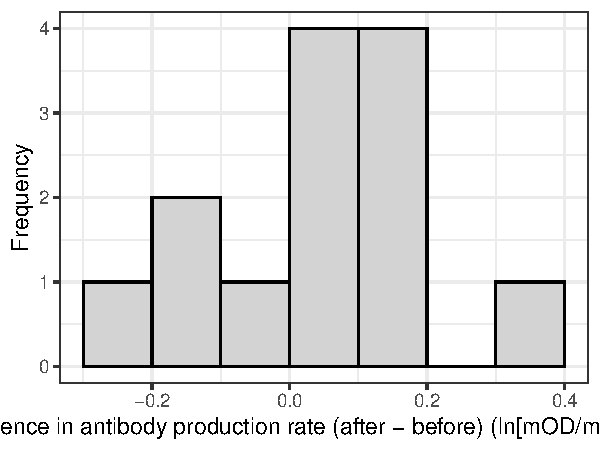
\includegraphics{BIOL202_files/figure-latex/unnamed-chunk-85-1.pdf}
\caption{\label{fig:unnamed-chunk-85}Histogram of the differences in antibody production rate before and after the testosterone treatment}
\end{figure}

With such a small sample size (13), the histogram is not particularly informative. But we do see most observations are just above zero.

\textbf{OPTIONAL}

Another optional but nice way to visualize paired data is using a paired plot.

\begin{Shaded}
\begin{Highlighting}[]
\NormalTok{blackbird }\SpecialCharTok{\%\textgreater{}\%}
  \FunctionTok{ggplot}\NormalTok{(}\FunctionTok{aes}\NormalTok{(}\AttributeTok{x =}\NormalTok{ time, }\AttributeTok{y =}\NormalTok{ Antibody)) }\SpecialCharTok{+}
  \FunctionTok{geom\_point}\NormalTok{(}\AttributeTok{shape =} \DecValTok{1}\NormalTok{, }\AttributeTok{size =} \FloatTok{1.5}\NormalTok{) }\SpecialCharTok{+}
  \FunctionTok{geom\_line}\NormalTok{(}\FunctionTok{aes}\NormalTok{(}\AttributeTok{group =}\NormalTok{ blackbird), }\AttributeTok{color =} \StringTok{"grey"}\NormalTok{) }\SpecialCharTok{+}
  \FunctionTok{theme\_bw}\NormalTok{()}
\end{Highlighting}
\end{Shaded}

\begin{figure}
\centering
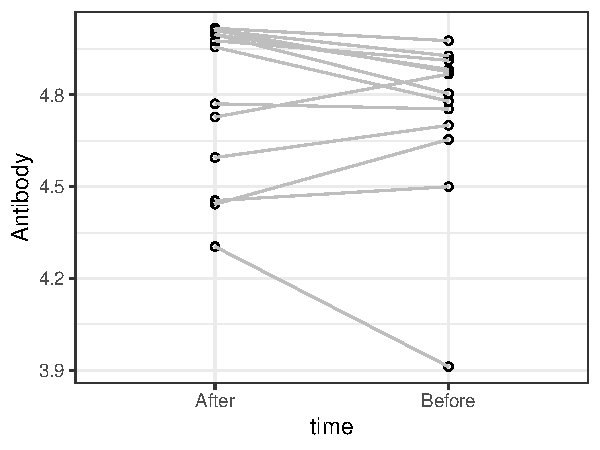
\includegraphics{BIOL202_files/figure-latex/unnamed-chunk-86-1.pdf}
\caption{\label{fig:unnamed-chunk-86}Paired plot of antibody production rate before and after the testosterone treatment}
\end{figure}

\textbf{OPTIONAL}

Notice that the ``After'' group is plotted on the left, which is a bit counter-intuitive. We could optionally change that by changing how R recognizes the ``order'' of the ``time'' variable:

\begin{Shaded}
\begin{Highlighting}[]
\NormalTok{blackbird}\SpecialCharTok{$}\NormalTok{time }\OtherTok{\textless{}{-}} \FunctionTok{ordered}\NormalTok{(blackbird}\SpecialCharTok{$}\NormalTok{time, }\AttributeTok{levels =} \FunctionTok{c}\NormalTok{(}\StringTok{"Before"}\NormalTok{, }\StringTok{"After"}\NormalTok{))}
\end{Highlighting}
\end{Shaded}

Then repeat the code above to create the paired plot.

\subsection{\texorpdfstring{Assumptions of the paired \emph{t}-test}{Assumptions of the paired t-test}}\label{assump_paried}

(Updated October 31, 2024)

The assumptions of the paired \emph{t}-test are the same as the assumptions for the one-sample \emph{t}-test, except they pertain to the \emph{difference}:

\begin{itemize}
\tightlist
\item
  the sampling units are randomly sampled from the population
\item
  the \emph{mean difference} has a normal distribution in the population (each group of measurements need not be normally distributed)
\end{itemize}

As instructed in the \hyperref[checknorm_assum]{checking assumptions} tutorial, we should use a normal quantile plot to visually check the normal distribution assumption, using the calculated differences.

\begin{Shaded}
\begin{Highlighting}[]
\NormalTok{blackbird.diffs }\SpecialCharTok{\%\textgreater{}\%}
  \FunctionTok{ggplot}\NormalTok{(}\FunctionTok{aes}\NormalTok{(}\AttributeTok{sample =}\NormalTok{ diffs)) }\SpecialCharTok{+}
  \FunctionTok{stat\_qq}\NormalTok{(}\AttributeTok{shape =} \DecValTok{1}\NormalTok{, }\AttributeTok{size =} \DecValTok{2}\NormalTok{) }\SpecialCharTok{+}
  \FunctionTok{stat\_qq\_line}\NormalTok{() }\SpecialCharTok{+}
  \FunctionTok{xlab}\NormalTok{(}\StringTok{"Normal quantile"}\NormalTok{) }\SpecialCharTok{+}
  \FunctionTok{ylab}\NormalTok{(}\StringTok{"Antibody production (ln[mOD/min]) 10\^{}{-}3"}\NormalTok{) }\SpecialCharTok{+}
  \FunctionTok{theme\_bw}\NormalTok{()}
\end{Highlighting}
\end{Shaded}

\begin{figure}
\centering
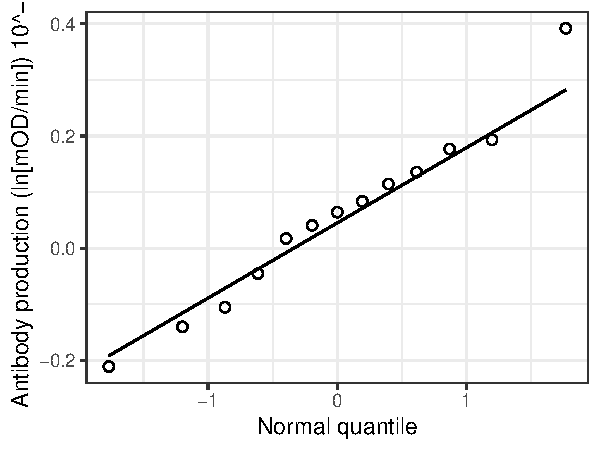
\includegraphics{BIOL202_files/figure-latex/unnamed-chunk-88-1.pdf}
\caption{\label{fig:unnamed-chunk-88}Normal quantile plot of the differences in antibody production rate before and after the testosterone treatment (ln{[}mOD/min{]}) 10\^{}-3.}
\end{figure}

We see that most of the lines are close to the line, with one point near the top right that is a bit off\ldots{}

A reasonable statement would be:

\begin{quote}
``The normal quantile plot shows that the data generally fall close to the line (except perhaps the highest value), indicating that the normality assumption is reasonably met.''
\end{quote}

But if you're feeling uncertain, we can follow this with a \textbf{Shapiro-Wilk Normality Test}, which tests the null hypothesis that the data are sampled from a normal distribution.

\begin{Shaded}
\begin{Highlighting}[]
\NormalTok{shapiro.result }\OtherTok{\textless{}{-}} \FunctionTok{shapiro.test}\NormalTok{(blackbird.diffs}\SpecialCharTok{$}\NormalTok{diffs)}
\NormalTok{shapiro.result.tidy }\OtherTok{\textless{}{-}} \FunctionTok{tidy}\NormalTok{(shapiro.result)}
\NormalTok{shapiro.result.tidy}
\end{Highlighting}
\end{Shaded}

\begin{verbatim}
## # A tibble: 1 x 3
##   statistic p.value method                     
##       <dbl>   <dbl> <chr>                      
## 1    0.9781  0.9688 Shapiro-Wilk normality test
\end{verbatim}

Given that the \emph{P}-value is large (and much greater than 0.05), there is no reason to reject the null hypothesis. Thus, our normality assumption is met.

When testing the normality assumption using the Shapiro-Wilk test, there is no need to conduct all the steps associated with a hypothesis test. Simply report the results of the test (the test statistic value and the associated \emph{P}-value).

For instance:

\begin{quote}
``A Shapiro-Wilk test revealed no evidence against the assumption that the data are drawn from a normal distribution (\emph{W} = 0.98, \emph{P}-value = 0.969).''
\end{quote}

\subsection{Conduct the test}\label{conduct_paired}

We can conduct a \textbf{paired t-test} in two different ways:

\begin{itemize}
\item
  conduct a one-sample \emph{t}-test on the \emph{differences} using the \texttt{t.test} function and methods you learned in a \hyperref[onesamp_t_test]{previous tutorial}.
\item
  conduct a paired \emph{t}-test using the \texttt{t.test} function and the argument \texttt{paired\ =\ TRUE}.
\end{itemize}

\textbf{(1) One-sample \emph{t}-test on the differences}

Let's proceed with the test as we've \hyperref[onesamp_t_test]{previously learned}.

Here we make sure to set the null hypothesized value of ``mu'' to zero in the argument for the \texttt{t.test} function:

\begin{Shaded}
\begin{Highlighting}[]
\NormalTok{blackbird.ttest }\OtherTok{\textless{}{-}}\NormalTok{ blackbird.diffs }\SpecialCharTok{\%\textgreater{}\%}
  \FunctionTok{select}\NormalTok{(diffs) }\SpecialCharTok{\%\textgreater{}\%}
  \FunctionTok{t.test}\NormalTok{(}\AttributeTok{mu =} \DecValTok{0}\NormalTok{, }\AttributeTok{alternative =} \StringTok{"two.sided"}\NormalTok{, }\AttributeTok{conf.level =} \FloatTok{0.95}\NormalTok{) }
\end{Highlighting}
\end{Shaded}

Now have a look at the result:

\begin{Shaded}
\begin{Highlighting}[]
\NormalTok{blackbird.ttest}
\end{Highlighting}
\end{Shaded}

\begin{verbatim}
## 
##  One Sample t-test
## 
## data:  .
## t = 1.2435, df = 12, p-value = 0.2374
## alternative hypothesis: true mean is not equal to 0
## 95 percent confidence interval:
##  -0.04134676  0.15128638
## sample estimates:
##  mean of x 
## 0.05496981
\end{verbatim}

The observed \emph{P}-value for our test is larger than our \(\alpha\) level of 0.05. We therefore fail to reject the null hypothesis.

The values of \emph{t} and of the lower and upper confidence limits may be reversed in sign, if you conducted your calculation of differences in the alternative way. Specifically, you may get \emph{t} = -1.2434925, and confidence limits of -0.1512864 and 0.0413468. This is totally fine!

\textbf{(2) Paired \emph{t}-test}

(Updated October 31, 2024)

Here again we'll use the wide-format tibble \texttt{blackbird.diffs}, using this approach:

\begin{Shaded}
\begin{Highlighting}[]
\NormalTok{blackbird.paired.ttest }\OtherTok{\textless{}{-}} \FunctionTok{t.test}\NormalTok{(}\AttributeTok{x =}\NormalTok{ blackbird.diffs}\SpecialCharTok{$}\NormalTok{Before, }\AttributeTok{y =}\NormalTok{ blackbird.diffs}\SpecialCharTok{$}\NormalTok{After,}
       \AttributeTok{paired =} \ConstantTok{TRUE}\NormalTok{, }\AttributeTok{alternative =} \StringTok{\textquotesingle{}two.sided\textquotesingle{}}\NormalTok{, }\AttributeTok{conf.level =} \FloatTok{0.95}\NormalTok{)}
\end{Highlighting}
\end{Shaded}

Here's an explanation:

\begin{itemize}
\tightlist
\item
  we create a new object ``blackbird.paried.ttest'' to store our results in
\item
  we run the \texttt{t.test} function with the arguments as follows:

  \begin{itemize}
  \tightlist
  \item
    we specify x equal to the ``Before'' variable, and y equal to the ``After'' variable
  \item
    we have the ``paired = TRUE'' argument, telling the function that this is a paired design
  \item
    we specify that this is a two-sided test with ``alternative = `two.sided'
  \item
    finally we use ``conf.level = 0.95'' which corresponds to an \(\alpha = 0.05\)
  \end{itemize}
\end{itemize}

Let's look at the result:

\begin{Shaded}
\begin{Highlighting}[]
\NormalTok{blackbird.paired.ttest}
\end{Highlighting}
\end{Shaded}

\begin{verbatim}
## 
##  Paired t-test
## 
## data:  blackbird.diffs$Before and blackbird.diffs$After
## t = -1.2435, df = 12, p-value = 0.2374
## alternative hypothesis: true mean difference is not equal to 0
## 95 percent confidence interval:
##  -0.15128638  0.04134676
## sample estimates:
## mean difference 
##     -0.05496981
\end{verbatim}

The output is identical to what we got when we applied a 1-sample \emph{t}-test on the differences!

The values of \emph{t} and of the lower and upper confidence limits may be reversed in sign, if you conducted your calculation of differences in the alternative way. Specifically, you may get \emph{t} = -1.2434925, and confidence limits of -0.1512864 and 0.0413468. This is totally fine!

\subsection{Concluding statement}\label{concl_paired}

Here's an example of a reasonable concluding statement, and this can apply for either of the two methods used above (note that in either case we call the test a ``paired \emph{t}-test, even if we used the one-sample \emph{t}-test on the differences):

\begin{quote}
We have no reason to reject the null hypothesis that the mean change in antibody production after testosterone implants was zero (paired \emph{t}-test; \emph{t} = -1.24; df = 12; \emph{P} = 0.237; 95\% confidence interval for the difference: -0.151 \(< \mu_d <\) 0.041).
\end{quote}

\section{\texorpdfstring{Two sample \emph{t}-test}{Two sample t-test}}\label{twosamp_ttest}

Have a look at the \texttt{students} dataset:

\begin{Shaded}
\begin{Highlighting}[]
\NormalTok{students }\SpecialCharTok{\%\textgreater{}\%}
  \FunctionTok{skim\_without\_charts}\NormalTok{()}
\end{Highlighting}
\end{Shaded}

\label{tab:unnamed-chunk-89}Data summary

Name

Piped data

Number of rows

154

Number of columns

6

\_\_\_\_\_\_\_\_\_\_\_\_\_\_\_\_\_\_\_\_\_\_\_

Column type frequency:

character

3

numeric

3

\_\_\_\_\_\_\_\_\_\_\_\_\_\_\_\_\_\_\_\_\_\_\_\_

Group variables

None

\textbf{Variable type: character}

skim\_variable

n\_missing

complete\_rate

min

max

empty

n\_unique

whitespace

Dominant\_hand

0

1

1

1

0

2

0

Dominant\_foot

0

1

1

1

0

2

0

Dominant\_eye

0

1

1

1

0

2

0

\textbf{Variable type: numeric}

skim\_variable

n\_missing

complete\_rate

mean

sd

p0

p25

p50

p75

p100

height\_cm

0

1

171.97

10.03

150

165.00

171.48

180.0

210.8

head\_circum\_cm

0

1

56.04

6.41

21

55.52

57.00

58.5

63.0

Number\_of\_siblings

0

1

1.71

1.05

0

1.00

2.00

2.0

6.0

These data include measurements taken on 154 students in BIOL202 a few years ago.

We'll use the ``height'' and ``Dominant\_eye'' variables for this section.

\textbf{OPTIONAL}

Note that the categories in the \texttt{Dominant\_eye} variable are ``l'' and ``r'', denoting ``left'' and ``right''.

We can use the \texttt{unique} function to tell us all unique values of a categorical variable:

\begin{Shaded}
\begin{Highlighting}[]
\NormalTok{students }\SpecialCharTok{\%\textgreater{}\%} 
  \FunctionTok{select}\NormalTok{(Dominant\_eye) }\SpecialCharTok{\%\textgreater{}\%}
  \FunctionTok{unique}\NormalTok{()}
\end{Highlighting}
\end{Shaded}

\begin{verbatim}
## # A tibble: 2 x 1
##   Dominant_eye
##   <chr>       
## 1 r           
## 2 l
\end{verbatim}

Let's change these to be more informative, ``Left'' and ``Right''.

We can do this with the \texttt{recode\_factor} function from the \texttt{dplyr} package (part of the \texttt{tidyverse}), in conjunction with the familiar \texttt{mutate} function used to create a new variable (though here we're just over-writing an existing variable):

\begin{Shaded}
\begin{Highlighting}[]
\NormalTok{students }\OtherTok{\textless{}{-}}\NormalTok{ students }\SpecialCharTok{\%\textgreater{}\%}
  \FunctionTok{mutate}\NormalTok{(}\AttributeTok{Dominant\_eye =} \FunctionTok{recode\_factor}\NormalTok{(Dominant\_eye, }\AttributeTok{r =} \StringTok{"Right"}\NormalTok{, }\AttributeTok{l =} \StringTok{"Left"}\NormalTok{))}
\end{Highlighting}
\end{Shaded}

\subsection{Hypothesis statement}\label{twosamp_hyp}

H\textsubscript{0}: Mean height is the same among students with left dominant eyes and right dominant eyes (\(\mu_L = \mu_R\)).\\
H\textsubscript{A}: Mean height is not the same among students with left dominant eyes and right dominant eyes (\(\mu_L \ne \mu_R\)).

Steps to a hypothesis test:

\begin{itemize}
\tightlist
\item
  We'll use an \(\alpha\) level of 0.05.\\
\item
  It is a two-tailed alternative hypothesis
\item
  We'll provide a table of descriptive statistics for each group
\item
  We'll visualize the data, and interpret the output
\item
  We'll use a 2-sample \emph{t}-test to test the null hypothesis, because we're dealing with numerical measurements taken on independent within two independent groups, and drawing inferences about population means \(\mu\) using sample data\\
\item
  We'll check the assumptions of the test (see below)
\item
  We'll calculate our test statistic
\item
  We'll calculate the \emph{P}-value associated with our test statistic
\item
  We'll calculate a 95\% confidence interval for the difference (\(\mu_L - \mu_R\))
\item
  We'll provide a good concluding statement that includes a 95\% confidence interval for the mean difference (\(\mu_L - \mu_R\))
\end{itemize}

\subsection{A table of descriptive statistics}\label{stats_2samp}

When we are analyzing a numeric response variable in relation to a categorical variable with two or more categories, it's good practice to provide a table of summary (or ``descriptive'') statistics (including confidence intervals for the mean) for the numeric variable grouped by the categories.

In a previous \hyperref[desc_numeric_var_cat]{tutorial} we learned how to calculate descriptive statistics for a numeric variable grouped by a categorical variable. In another \hyperref[conf_precision]{tutorial} we also learned how to calculate confidence intervals for a numeric variable.

We've also learned that the \texttt{t.test} function returns a confidence interval for us.

Let's use all these skills to generate a table of summary statistics for the ``height\_cm'' variable, grouped by ``Dominant\_eye'':

\begin{Shaded}
\begin{Highlighting}[]
\NormalTok{height.stats }\OtherTok{\textless{}{-}}\NormalTok{ students }\SpecialCharTok{\%\textgreater{}\%}
  \FunctionTok{group\_by}\NormalTok{(Dominant\_eye) }\SpecialCharTok{\%\textgreater{}\%}
  \FunctionTok{summarise}\NormalTok{(}
    \AttributeTok{Count =} \FunctionTok{n}\NormalTok{() }\SpecialCharTok{{-}}\NormalTok{ naniar}\SpecialCharTok{::}\FunctionTok{n\_miss}\NormalTok{(height\_cm),}
    \AttributeTok{Count\_NA =}\NormalTok{ naniar}\SpecialCharTok{::}\FunctionTok{n\_miss}\NormalTok{(height\_cm), }
    \AttributeTok{Mean =} \FunctionTok{mean}\NormalTok{(height\_cm, }\AttributeTok{na.rm =} \ConstantTok{TRUE}\NormalTok{),}
    \AttributeTok{SD =} \FunctionTok{sd}\NormalTok{(height\_cm, }\AttributeTok{na.rm =} \ConstantTok{TRUE}\NormalTok{),}
    \AttributeTok{SEM =}\NormalTok{ SD}\SpecialCharTok{/}\FunctionTok{sqrt}\NormalTok{(Count),}
    \AttributeTok{Low\_95\_CL =} \FunctionTok{t.test}\NormalTok{(height\_cm, }\AttributeTok{conf.level =} \FloatTok{0.95}\NormalTok{)}\SpecialCharTok{$}\NormalTok{conf.int[}\DecValTok{1}\NormalTok{],}
    \AttributeTok{Up\_95\_CL =} \FunctionTok{t.test}\NormalTok{(height\_cm, }\AttributeTok{conf.level =} \FloatTok{0.95}\NormalTok{)}\SpecialCharTok{$}\NormalTok{conf.int[}\DecValTok{2}\NormalTok{]}
\NormalTok{  )}
\end{Highlighting}
\end{Shaded}

The only unfamiliar code in the preceding chunk is the last two lines:

\begin{itemize}
\tightlist
\item
  we use the \texttt{t.test} function to calculate the lower and upper confidence limits. Specifically:

  \begin{itemize}
  \tightlist
  \item
    after the closing parenthesis to the \texttt{t.test} function, we include ``\$conf.int{[}1{]}'', and this simply extracts the first value (lower limit) of the calculated confidence limits from the \texttt{t.test} output
  \item
    we do the same for the upper confidence limit, but this time we include ``\$conf.int{[}2{]}''
  \end{itemize}
\end{itemize}

Now let's have a look at the table, using the \texttt{kable} function to produce a nice table.

\textbf{NOTE} here I am rotating the table so that it fits on the page. To do this, use the \texttt{t} function as follows:

\begin{Shaded}
\begin{Highlighting}[]
\FunctionTok{kable}\NormalTok{(}\FunctionTok{t}\NormalTok{(height.stats), }\AttributeTok{digits =} \DecValTok{4}\NormalTok{)}
\end{Highlighting}
\end{Shaded}

Dominant\_eye

Right

Left

Count

106

48

Count\_NA

0

0

Mean

172.8368

170.0598

SD

10.397638

8.964659

SEM

1.009908

1.293937

Low\_95\_CL

170.8343

167.4567

Up\_95\_CL

174.8393

172.6629

It is best to \textbf{NOT rotate the table}, but it is fine to do so if your table goes off the page!

We'll learn a better way to get around this later.

\subsection{\texorpdfstring{A graph to accompany a 2-sample \emph{t}-test}{A graph to accompany a 2-sample t-test}}\label{graph_2samp}

We learned in an earlier \hyperref[numeric_vs_cat]{tutorial} that we can use a stripchart, violin plot, or boxplot to visualize the association between a numerical response variable and a categorical explanatory variable. Better yet, we can do the \hyperref[bestplot]{combined violin \& boxplot}.

Here we want to visualize height in relation to dominant eye (Left or Right). We can use the information provided in our descriptive stats table to get the sample sizes for the groups (which we need to report in the figure heading).

\begin{Shaded}
\begin{Highlighting}[]
\NormalTok{students }\SpecialCharTok{\%\textgreater{}\%} 
  \FunctionTok{ggplot}\NormalTok{(}\FunctionTok{aes}\NormalTok{(}\AttributeTok{x =}\NormalTok{ Dominant\_eye, }\AttributeTok{y =}\NormalTok{ height\_cm)) }\SpecialCharTok{+}
  \FunctionTok{geom\_violin}\NormalTok{() }\SpecialCharTok{+}
  \FunctionTok{geom\_boxplot}\NormalTok{(}\AttributeTok{width =} \FloatTok{0.1}\NormalTok{) }\SpecialCharTok{+} 
  \FunctionTok{geom\_jitter}\NormalTok{(}\AttributeTok{colour =} \StringTok{"grey"}\NormalTok{, }\AttributeTok{size =} \DecValTok{1}\NormalTok{, }\AttributeTok{shape =} \DecValTok{1}\NormalTok{, }\AttributeTok{width =} \FloatTok{0.15}\NormalTok{) }\SpecialCharTok{+}
  \FunctionTok{xlab}\NormalTok{(}\StringTok{"Dominant eye"}\NormalTok{) }\SpecialCharTok{+}
  \FunctionTok{ylab}\NormalTok{(}\StringTok{"Height (cm)"}\NormalTok{) }\SpecialCharTok{+}
  \FunctionTok{theme\_bw}\NormalTok{()}
\end{Highlighting}
\end{Shaded}

\begin{figure}
\centering
\includegraphics{BIOL202_files/figure-latex/unnamed-chunk-92-1.pdf}
\caption{\label{fig:unnamed-chunk-92}Violin and boxplot of the heights of students with right (n = 106) and left (n = 48) dominant eyes. Boxes delimit the first to third quartiles, bold lines represent the group medians, and whiskers extend to 1.5 times the IQR. Points beyond whiskers are extreme observations.}
\end{figure}

\textbf{Interpretation}

\begin{quote}
We can see in the preceding figure that heights are generally similar between students with left dominant eyes and those with right dominant eyes. However, it appears that the spread of the heights is greater among students with right dominant eyes. We will need to be careful about the equal-variance assumption for the 2-sample \emph{t}-test.
\end{quote}

\subsection{\texorpdfstring{Assumptions of the 2-sample \emph{t}-test}{Assumptions of the 2-sample t-test}}\label{twosamp_assump}

The assumptions of the 2-sample \emph{t}-test are as follows:

\begin{itemize}
\tightlist
\item
  each of the two samples is a random sample from its population
\item
  the numerical variable is normally distributed in each population
\item
  the variance (and thus standard deviation) of the numerical variable is the same in both populations
\end{itemize}

\textbf{Test for normality}

Now let's check the normality assumption by plotting a normal quantile plot for each group.

We'll introduce the \texttt{facet\_grid} function that enables plotting of side-by-side panels according to a grouping variable.

\begin{Shaded}
\begin{Highlighting}[]
\NormalTok{students }\SpecialCharTok{\%\textgreater{}\%}
  \FunctionTok{ggplot}\NormalTok{(}\FunctionTok{aes}\NormalTok{(}\AttributeTok{sample =}\NormalTok{ height\_cm)) }\SpecialCharTok{+}
  \FunctionTok{stat\_qq}\NormalTok{(}\AttributeTok{shape =} \DecValTok{1}\NormalTok{, }\AttributeTok{size =} \DecValTok{2}\NormalTok{) }\SpecialCharTok{+}
  \FunctionTok{stat\_qq\_line}\NormalTok{() }\SpecialCharTok{+}
  \FunctionTok{facet\_grid}\NormalTok{(}\SpecialCharTok{\textasciitilde{}}\NormalTok{ Dominant\_eye) }\SpecialCharTok{+}
  \FunctionTok{xlab}\NormalTok{(}\StringTok{"Normal quantile"}\NormalTok{) }\SpecialCharTok{+}
  \FunctionTok{ylab}\NormalTok{(}\StringTok{"Height (cm)"}\NormalTok{) }\SpecialCharTok{+}
  \FunctionTok{theme\_bw}\NormalTok{()}
\end{Highlighting}
\end{Shaded}

\begin{figure}
\centering
\includegraphics{BIOL202_files/figure-latex/unnamed-chunk-93-1.pdf}
\caption{\label{fig:unnamed-chunk-93}Normal quantile plots of height for students with right (n = 106) or left (n = 48) dominant eyes.}
\end{figure}

A reasonable statement would be:

\begin{quote}
``The normal quantile plots show that student height is generally normally distributed for students with left or right dominant eyes. There is one observation among the right-dominant eye students that is a bit off the line.''
\end{quote}

\textbf{Test for equal variances}

Now we need to test the assumption of equal variance among the groups, using Levene's Test as we learned in the \hyperref[levenetest]{checking assumptions} tutorial.

\begin{Shaded}
\begin{Highlighting}[]
\NormalTok{height.vartest }\OtherTok{\textless{}{-}} \FunctionTok{leveneTest}\NormalTok{(height\_cm }\SpecialCharTok{\textasciitilde{}}\NormalTok{ Dominant\_eye, }\AttributeTok{data =}\NormalTok{ students)}
\NormalTok{height.vartest}
\end{Highlighting}
\end{Shaded}

\begin{verbatim}
## Levene's Test for Homogeneity of Variance (center = median)
##        Df F value Pr(>F)
## group   1   0.907 0.3424
##       152
\end{verbatim}

It uses a test statistic ``F'', and we see here that the \emph{P}-value associated with the test statistic is larger than 0.05, so we don't reject the implied null hypothesis that the variances are equal.

We state ``A Levene's test showed no evidence against the assumption of equal variance (\emph{F} = 0.91; \emph{P}-value = 0.342).''

Thus, we'll proceed with conducting the 2-sample \emph{t}-test.

\subsection{\texorpdfstring{Conduct the 2-sample \emph{t}-test}{Conduct the 2-sample t-test}}\label{conduct_2samptest}

We use the \texttt{t.test} function again for this test.

\begin{Shaded}
\begin{Highlighting}[]
\NormalTok{height.ttest }\OtherTok{\textless{}{-}}\NormalTok{ students }\SpecialCharTok{\%\textgreater{}\%}
  \FunctionTok{t.test}\NormalTok{(height\_cm }\SpecialCharTok{\textasciitilde{}}\NormalTok{ Dominant\_eye, }
         \AttributeTok{data =}\NormalTok{ ., }\AttributeTok{var.equal =} \ConstantTok{TRUE}\NormalTok{, }\AttributeTok{conf.level =} \FloatTok{0.95}\NormalTok{)}
\end{Highlighting}
\end{Shaded}

The only difference from the implementation used in the paired \emph{t}-test is:

\begin{itemize}
\tightlist
\item
  we include the ``var.equal = TRUE'' argument
\end{itemize}

We again include the argument ``data = .'', which tells the \texttt{t.test} function that whatever data was passed to it from the preceding line is what will be used

We'll learn a bit later what to due when the equal variance assumption is not met.

Let's look at the result:

\begin{Shaded}
\begin{Highlighting}[]
\NormalTok{height.ttest}
\end{Highlighting}
\end{Shaded}

\begin{verbatim}
## 
##  Two Sample t-test
## 
## data:  height_cm by Dominant_eye
## t = 1.6, df = 152, p-value = 0.1117
## alternative hypothesis: true difference in means between group Right and group Left is not equal to 0
## 95 percent confidence interval:
##  -0.6521529  6.2061545
## sample estimates:
## mean in group Right  mean in group Left 
##            172.8368            170.0598
\end{verbatim}

We see that the test produced a \emph{P}-value greater than \(\alpha\), so we fail to reject the null hypothesis.

Note also that the output includes a \textbf{confidence interval} for the \emph{difference} in group means. We need to include this in our concluding statement.

\subsection{Concluding statement}\label{concl_2samp}

Here's an example of a concluding statement:

\begin{quote}
On average, students with left dominant eyes are similar in height to students with right dominant eyes (Figure 19.4) (2-sample \emph{t}-test; \emph{t} = 1.6; df = 152; \emph{P}-value = 0.112; 95\% confidence interval for the difference in height -0.652 \(< \mu_d <\) 6.206).
\end{quote}

\section{When assumptions aren't met}\label{assumpbad_2samp}

If the \textbf{normal distribution assumption} is violated, and you are unable to find a transformation that works (see the \hyperref[assumptions_packages_data]{Checking assumptions and data transformations} tutorial), then you can try a non-parametric test.

A tutorial on non-parametric tests is under development, but will not be deployed until 2023. Consult chapter 13 in the Whitlock \& Schluter text, and this \href{https://whitlockschluter3e.zoology.ubc.ca/RExamples/Rcode_Chapter_13.html\#new_methods_on_this_page}{website} for some R examples.

If the \textbf{equal-variance assumption} is violated for the 2-sample \emph{t}-test, then you can set the ``var.equal'' argument to ``FALSE'' in the \texttt{t.test} function, in which case the function implements a ``Welch's \emph{t}-test''.

For instance, let's pretend that the height data did not exhibit equal variance among left- and right- dominant eye students, here's the appropriate code:

\begin{Shaded}
\begin{Highlighting}[]
\NormalTok{height.ttest.unequal.var }\OtherTok{\textless{}{-}}\NormalTok{ students }\SpecialCharTok{\%\textgreater{}\%}
  \FunctionTok{t.test}\NormalTok{(height\_cm }\SpecialCharTok{\textasciitilde{}}\NormalTok{ Dominant\_eye, }
         \AttributeTok{data =}\NormalTok{ ., }\AttributeTok{var.equal =} \ConstantTok{FALSE}\NormalTok{, }\AttributeTok{conf.level =} \FloatTok{0.95}\NormalTok{)}
\NormalTok{height.ttest.unequal.var}
\end{Highlighting}
\end{Shaded}

\begin{verbatim}
## 
##  Welch Two Sample t-test
## 
## data:  height_cm by Dominant_eye
## t = 1.6919, df = 104.37, p-value = 0.09366
## alternative hypothesis: true difference in means between group Right and group Left is not equal to 0
## 95 percent confidence interval:
##  -0.4778181  6.0318197
## sample estimates:
## mean in group Right  mean in group Left 
##            172.8368            170.0598
\end{verbatim}

\chapter{Checking assumptions and data transformations}\label{assumptions_trans}

\textbf{Tutorial learning objectives}

\begin{itemize}
\tightlist
\item
  Learn how to check the normality assumption

  \begin{itemize}
  \tightlist
  \item
    Normal quantile plots
  \item
    Shapiro-Wilk test for normality
  \end{itemize}
\item
  Learn how to check the equal variance assumption

  \begin{itemize}
  \tightlist
  \item
    Levene's Test
  \end{itemize}
\item
  Learn how to transform the response variable to help meet assumptions

  \begin{itemize}
  \tightlist
  \item
    log-transform
  \item
    Dealing with zeroes\\
  \item
    log bases
  \item
    back-transforming log data
  \item
    logit transform
  \item
    back-transforming logit data
  \item
    when to back-transform?
  \end{itemize}
\end{itemize}

Most statistical tests, such as the \(\chi\)\textsuperscript{2} goodness of fit test, the \(\chi\)\textsuperscript{2} contingency test, \emph{t}-test, ANOVA, Pearson correlation, and least-squares regression, have assumptions that must be met. For example, the one-sample \emph{t}-test requires that the variable is normally distributed in the population, and least-squares regression requires that the residuals from the regression be normally distributed. In this tutorial we'll learn ways to check the assumption that the variable is normally distributed in the population.

We'll also learn how transforming a variable can sometimes help satisfy assumptions, in which case the analysis is conducted on the transformed variable.

\section{Load packages and import data}\label{assumptions_packages_data}

Load the usual packages, and \texttt{broom}, which has been used in some tutorials:

\begin{Shaded}
\begin{Highlighting}[]
\FunctionTok{library}\NormalTok{(tidyverse)}
\FunctionTok{library}\NormalTok{(skimr)}
\FunctionTok{library}\NormalTok{(broom)}
\end{Highlighting}
\end{Shaded}

And we need these two packages also: \texttt{car}, \texttt{boot}. Install these if you don't have them (as per instructions in a previous \hyperref[package_install]{tutorial}), then load them:

\begin{Shaded}
\begin{Highlighting}[]
\FunctionTok{library}\NormalTok{(car)  }
\FunctionTok{library}\NormalTok{(boot)}
\end{Highlighting}
\end{Shaded}

The ``marine.csv'' dataset is discussed in example 13.1 in the text book. The ``flowers.csv'' dataset is described below. The ``students.csv'' data include data about BIOL202 students from a few years ago.

Let's make sure to treat any categorical variables as factor variables, using the ``stringsAsFactors = T'' argument:

\begin{Shaded}
\begin{Highlighting}[]
\NormalTok{marine }\OtherTok{\textless{}{-}} \FunctionTok{read\_csv}\NormalTok{(}\StringTok{"https://raw.githubusercontent.com/ubco{-}biology/BIOL202/main/data/marine.csv"}\NormalTok{)}
\end{Highlighting}
\end{Shaded}

\begin{verbatim}
## Rows: 32 Columns: 1
## -- Column specification --------------------------------------------------------
## Delimiter: ","
## dbl (1): biomassRatio
## 
## i Use `spec()` to retrieve the full column specification for this data.
## i Specify the column types or set `show_col_types = FALSE` to quiet this message.
\end{verbatim}

\begin{Shaded}
\begin{Highlighting}[]
\NormalTok{flowers }\OtherTok{\textless{}{-}} \FunctionTok{read\_csv}\NormalTok{(}\StringTok{"https://raw.githubusercontent.com/ubco{-}biology/BIOL202/main/data/flowers.csv"}\NormalTok{)}
\end{Highlighting}
\end{Shaded}

\begin{verbatim}
## Rows: 30 Columns: 1
## -- Column specification --------------------------------------------------------
## Delimiter: ","
## dbl (1): propFertile
## 
## i Use `spec()` to retrieve the full column specification for this data.
## i Specify the column types or set `show_col_types = FALSE` to quiet this message.
\end{verbatim}

\begin{Shaded}
\begin{Highlighting}[]
\NormalTok{students }\OtherTok{\textless{}{-}} \FunctionTok{read\_csv}\NormalTok{(}\StringTok{"https://raw.githubusercontent.com/ubco{-}biology/BIOL202/main/data/students.csv"}\NormalTok{)}
\end{Highlighting}
\end{Shaded}

\begin{verbatim}
## Rows: 154 Columns: 6
## -- Column specification --------------------------------------------------------
## Delimiter: ","
## chr (3): Dominant_hand, Dominant_foot, Dominant_eye
## dbl (3): height_cm, head_circum_cm, Number_of_siblings
## 
## i Use `spec()` to retrieve the full column specification for this data.
## i Specify the column types or set `show_col_types = FALSE` to quiet this message.
\end{verbatim}

Explore the \texttt{marine} and \texttt{flowers} datasets:

\begin{Shaded}
\begin{Highlighting}[]
\NormalTok{marine }\SpecialCharTok{\%\textgreater{}\%}
  \FunctionTok{skim\_without\_charts}\NormalTok{()}
\end{Highlighting}
\end{Shaded}

(\#tab:skim\_marine)Data summary

Name

Piped data

Number of rows

32

Number of columns

1

\_\_\_\_\_\_\_\_\_\_\_\_\_\_\_\_\_\_\_\_\_\_\_

Column type frequency:

numeric

1

\_\_\_\_\_\_\_\_\_\_\_\_\_\_\_\_\_\_\_\_\_\_\_\_

Group variables

None

\textbf{Variable type: numeric}

skim\_variable

n\_missing

complete\_rate

mean

sd

p0

p25

p50

p75

p100

biomassRatio

0

1

1.73

0.75

0.83

1.27

1.49

1.85

4.25

\begin{Shaded}
\begin{Highlighting}[]
\NormalTok{flowers }\SpecialCharTok{\%\textgreater{}\%}
  \FunctionTok{skim\_without\_charts}\NormalTok{()}
\end{Highlighting}
\end{Shaded}

(\#tab:skim\_flowers)Data summary

Name

Piped data

Number of rows

30

Number of columns

1

\_\_\_\_\_\_\_\_\_\_\_\_\_\_\_\_\_\_\_\_\_\_\_

Column type frequency:

numeric

1

\_\_\_\_\_\_\_\_\_\_\_\_\_\_\_\_\_\_\_\_\_\_\_\_

Group variables

None

\textbf{Variable type: numeric}

skim\_variable

n\_missing

complete\_rate

mean

sd

p0

p25

p50

p75

p100

propFertile

0

1

0.47

0.33

0.01

0.13

0.49

0.75

0.99

\section{Checking the normality assumption}\label{checknorm_assum}

Statistical tests such as the one-sample \emph{t} test assume that the response variable of interest is normally distributed in the population.

Many biological variables are known to be normally distributed in the population, but for some variables we can't be sure. Given a proper random sample from the population, of sufficient sample size, we can assume that the frequency distribution of our sample data will, to reasonable degree, reflect the frequency distribution of the variable in the population.

Importantly, tests such as the one-sample \emph{t} test are somewhat \textbf{robust} to minor violations of this assumption. Nevertheless, it is best practice to be transparent in testing the assumption, i.e.~showing how it was tested and exactly what was found.

\subsection{Normal quantile plots}\label{quantile_plots}

The most straightforward way to check the normality assumption is to visualize the data using a \textbf{normal quantile plot}.

The \texttt{ggplot2} package (loaded with the \texttt{tidyverse} package) has plotting functions for this, called \texttt{stat\_qq} and \texttt{stat\_qq\_line}:

\begin{verbatim}
?stat_qq
?stat_qq_line
\end{verbatim}

For details about what Normal Quantile Plots are, and how they're constructed, consult this informative \href{https://data.library.virginia.edu/understanding-q-q-plots/}{link}.

If the frequency distribution were normally distributed, points would fall close to the straight line in the normal quantile plot.

Check out this example showing simulated data drawn from a normal distribution:

\begin{figure}
\centering
\includegraphics{BIOL202_files/figure-latex/unnamed-chunk-100-1.pdf}
\caption{\label{fig:unnamed-chunk-100}Example of a normal quantile plot for a variable that is normally distributed.}
\end{figure}

Now we'll use the \texttt{marine} dataset and its variable called \texttt{biomassRatio} to illustrate.

We'll first construct a histogram as you've \hyperref[vis_histogram]{learned previously}, just to see how the shape of the frequency distribution relates to the pattern seen in the normal quantile plot.

\begin{Shaded}
\begin{Highlighting}[]
\NormalTok{marine }\SpecialCharTok{\%\textgreater{}\%}
  \FunctionTok{ggplot}\NormalTok{(}\FunctionTok{aes}\NormalTok{(}\AttributeTok{x =}\NormalTok{ biomassRatio)) }\SpecialCharTok{+}
  \FunctionTok{geom\_histogram}\NormalTok{(}\AttributeTok{binwidth =} \FloatTok{0.5}\NormalTok{, }\AttributeTok{color =} \StringTok{"black"}\NormalTok{, }\AttributeTok{fill =} \StringTok{"lightgrey"}\NormalTok{, }
                 \AttributeTok{boundary =} \DecValTok{0}\NormalTok{, }\AttributeTok{closed =} \StringTok{"left"}\NormalTok{) }\SpecialCharTok{+}
  \FunctionTok{xlab}\NormalTok{(}\StringTok{"Biomass ratio"}\NormalTok{) }\SpecialCharTok{+}
  \FunctionTok{ylab}\NormalTok{(}\StringTok{"Frequency"}\NormalTok{) }\SpecialCharTok{+}
  \FunctionTok{theme\_bw}\NormalTok{()}
\end{Highlighting}
\end{Shaded}

\begin{figure}
\centering
\includegraphics{BIOL202_files/figure-latex/unnamed-chunk-101-1.pdf}
\caption{\label{fig:unnamed-chunk-101}The frequency distribution of the `biomass ratio' of 32 marine reserves.}
\end{figure}

Notice that the distribution is quite right-skewed (or ``postively skewed'').

Now the quantile plot:

\begin{Shaded}
\begin{Highlighting}[]
\NormalTok{marine }\SpecialCharTok{\%\textgreater{}\%} 
 \FunctionTok{ggplot}\NormalTok{(}\FunctionTok{aes}\NormalTok{(}\AttributeTok{sample =}\NormalTok{ biomassRatio)) }\SpecialCharTok{+}
  \FunctionTok{stat\_qq}\NormalTok{(}\AttributeTok{shape =} \DecValTok{1}\NormalTok{, }\AttributeTok{size =} \DecValTok{2}\NormalTok{) }\SpecialCharTok{+}
  \FunctionTok{stat\_qq\_line}\NormalTok{() }\SpecialCharTok{+}
  \FunctionTok{ylab}\NormalTok{(}\StringTok{"Biomass ratio"}\NormalTok{) }\SpecialCharTok{+}
  \FunctionTok{xlab}\NormalTok{(}\StringTok{"Normal quantile"}\NormalTok{) }\SpecialCharTok{+}
  \FunctionTok{theme\_bw}\NormalTok{()}
\end{Highlighting}
\end{Shaded}

\begin{figure}
\centering
\includegraphics{BIOL202_files/figure-latex/unnamed-chunk-102-1.pdf}
\caption{\label{fig:unnamed-chunk-102}Normal quantile plot of the `biomass ratio' of 32 marine reserves.}
\end{figure}

Notice that in the ``aes'' argument we use ``sample = biomassRatio''. This is new, and is only required for the normal quantile plot, specifically the subsequent \texttt{stat\_qq} and \texttt{stat\_qq\_line} functions.

Notice that normal quantile plot shows points deviating substantially from the straight line in the top-right part of the plot, and this corresponds to the right-skew in the histogram.

Clearly, the frequency distribution of the \texttt{biomassRatio} variable does not conform to a normal distribution.

Here's an example statement one could make when checking this assumption:

\begin{quote}
The assumption of normality was checked visually using a normal quantile plot, which showed that the data were clearly not normally distributed.
\end{quote}

\textbf{Important: }
Egregious deviations from the normality assumption will be clearly evident in normal quantile plots (as in the example above). If it is difficult to tell whether the data are normally distributed, then they probably are OK (at least sufficiently with respect to the assumption).

\subsection{Shapiro-Wilk test for normality}\label{shapirottest}

Although graphical assessments are usually sufficient for checking the normality assumption, one can conduct a formal statistical test of the null hypothesis that the data are sampled from a population having a normal distribution. The test is called the \textbf{Shapiro-Wilk test}.

The Shapiro-Wilk test is a type of goodness-of-fit test.

Sometimes the \textbf{Shapiro-Wilk test} is applied in a hypothesis testing framework, but when it is applied as part of checking assumptions for another statistical test (like we're doing here), one does not need to present it in a hypothesis test framework. However, the implied null hypothesis is that ``The data are sampled from a population having a normal distribution'', and one does interpret the resulting \emph{P}-value in the same way as usual, i.e.~in relation to an \(\alpha\) level (see below).

We'll make use of the \texttt{shapiro.test} function from base R stats package:

\begin{verbatim}
shapiro.test
\end{verbatim}

Let's use this on the \texttt{biomassRatio} variable in the ``marine'' dataset. We'll assign the output to an object called ``shapiro.result'', then we'll have a look at the results.

The output from the \texttt{shapiro.test} function is not ``tidy'', so we will use the \texttt{tidy} function from the \texttt{broom} package to make it tidy.

Here we go: we provide the function with the tibble name (``marine'') and the variable of interest after a ``\$'':

\begin{Shaded}
\begin{Highlighting}[]
\NormalTok{shapiro.result }\OtherTok{\textless{}{-}} \FunctionTok{shapiro.test}\NormalTok{(marine}\SpecialCharTok{$}\NormalTok{biomassRatio)}
\end{Highlighting}
\end{Shaded}

Now tidy the output:

\begin{Shaded}
\begin{Highlighting}[]
\NormalTok{shapiro.result.tidy }\OtherTok{\textless{}{-}} \FunctionTok{tidy}\NormalTok{(shapiro.result)}
\end{Highlighting}
\end{Shaded}

Now look at the results:

\begin{Shaded}
\begin{Highlighting}[]
\NormalTok{shapiro.result.tidy}
\end{Highlighting}
\end{Shaded}

\begin{verbatim}
## # A tibble: 1 x 3
##   statistic    p.value method                     
##       <dbl>      <dbl> <chr>                      
## 1    0.8175 0.00008851 Shapiro-Wilk normality test
\end{verbatim}

The tidy object includes:

\begin{itemize}
\tightlist
\item
  The value of the test statistic for the Shapriro-Wilk test (although it is not shown, this test statistic is indicated with a ``W'')
\item
  The \emph{P}-value associated with the test (``p.value'')
\item
  The name of the test used (``method'')
\end{itemize}

Given that the \emph{P}-value is less than a conventional \(\alpha\) level of 0.05, the test is telling us that the data do not conform to a normal distribution. Of course we already knew that from our visual assessments!

Here's an example statement:

\begin{quote}
The assumption of normality was checked visually using a normal quantile plot, and a Shapiro-Wilk test, which revealed evidence of non-normality (Shapiro-Wilk test, W = 0.82, \emph{P}-value \textless{} 0.001).
\end{quote}

\textbf{Important: }
Visual assessments of normality are preferred, because the outcome of the Shapiro-Wilk test is sensitive to sample size: a small sample size will often yield a false negative, whereas very large sample sizes could yield false positives more than it should.

\section{Checking the equal-variance assumption}\label{levenetest}

Some statistical tests, such as the 2-sample \emph{t}-test and ANOVA, assume that the variance (\(\sigma\)) of the numeric response variable is the same among the populations being compared.

For this we use the \textbf{Levene's test}, which we implement using the \texttt{leveneTest} function from the \texttt{car} package:

\begin{verbatim}
?leveneTest
\end{verbatim}

Like the Shapiro-Wilk test, the Levene's test can be applied in a hypothesis testing framework, but when it is used to evaluate the equal-variance assumption, it need not be.

Nevertheless, the \emph{implied} null hypothesis is that the variance of the numeric response variable is the same among the populations being compared. So in the case where a numeric variable is being compared among two groups, then the implied null hypothesis is that (\(\sigma\)(1) = \(\sigma\)(2). The usual \(\alpha\) level of 0.05 can be used.

We'll use the ``students'' dataset, and check whether \texttt{height\_cm} exhibits equal variance among students with different dominant eyes (left or right).

Let's look at the code, and explain after:

\begin{Shaded}
\begin{Highlighting}[]
\NormalTok{height.vartest }\OtherTok{\textless{}{-}} \FunctionTok{leveneTest}\NormalTok{(height\_cm }\SpecialCharTok{\textasciitilde{}}\NormalTok{ Dominant\_eye, }\AttributeTok{data =}\NormalTok{ students)}
\end{Highlighting}
\end{Shaded}

If you get a warning about a variable being ``coerced to factor'', that's OK! It is simply telling you that it took the categorical variable and treated it as a `factor' variable.

In the code chunk above we:

\begin{itemize}
\tightlist
\item
  assign the results to a new object called ``height.vartest''
\item
  use the \texttt{leveneTest} function, in which the arguments are:

  \begin{itemize}
  \tightlist
  \item
    the numeric response variable (``height\_cm'')
  \item
    then the ``\textasciitilde{}'' symbol
  \item
    then the categorical variable ``dominant\_eye''
  \item
    then the ``data = students'' specifies the data object name
  \end{itemize}
\end{itemize}

\textbf{TIP: }
The argument to the \texttt{leveneTest} function that is in the form \(Y\) \textasciitilde{} \(X\) is one we'll use several times.

Let's look at the results:

\begin{Shaded}
\begin{Highlighting}[]
\NormalTok{height.vartest}
\end{Highlighting}
\end{Shaded}

\begin{verbatim}
## Levene's Test for Homogeneity of Variance (center = median)
##        Df F value Pr(>F)
## group   1   0.907 0.3424
##       152
\end{verbatim}

The results include:

\begin{itemize}
\tightlist
\item
  the degrees of freedom for the test
\item
  the value of the test statistic ``F''
\item
  the \emph{P}-value associated with the test statistic
\end{itemize}

For the student height example, the \emph{P}-value is greater than the standard \(\alpha\) of 0.05, so there's no evidence against the assumption of equal variance.

A reasonable statement would be:

\begin{quote}
``A Levene's test showed no evidence against the assumption of equal variance (\emph{F} = 0.91; \emph{P}-value = 0.342).''
\end{quote}

\textbf{TIP: }
As part of your main statistical test, such as a two-sample \emph{t}-test or an ANOVA, you would typically provide a graph such as a \hyperref[numeric_vs_cat]{stripchart or violin plot} to visualize how the numeric response variable varies among the groups of the categorical explanatory variable. Such plots may often reveal that the spread of values of the response variable varies considerably among the groups, underscoring the need to check the equal variance assumption.

\section{Data transformations}\label{transform}

Here we learn how to transform numeric variables using two common methods:

\begin{itemize}
\tightlist
\item
  log-transform
\item
  logit-transform
\end{itemize}

There are many other types of transformations that can be performed, some of which are described in \textbf{Chapter 13} of the course text book.

Contrary to what is suggested in the text, it is better to use the ``logit'' transformation rather than the ``arcsin square-root'' transformation for proportion or percentage data, as described in this \href{http://onlinelibrary.wiley.com/doi/10.1890/10-0340.1/abstract}{article} by Warton and Hui (2011).

\subsection{Log-transform}\label{log_transform}

When one observes a right-skewed frequency distribution, as seen here in the marine biomass ratio data, a log-transformation often helps.

\begin{Shaded}
\begin{Highlighting}[]
\NormalTok{marine }\SpecialCharTok{\%\textgreater{}\%}
  \FunctionTok{ggplot}\NormalTok{(}\FunctionTok{aes}\NormalTok{(}\AttributeTok{x =}\NormalTok{ biomassRatio)) }\SpecialCharTok{+}
  \FunctionTok{geom\_histogram}\NormalTok{(}\AttributeTok{binwidth =} \FloatTok{0.5}\NormalTok{, }\AttributeTok{color =} \StringTok{"black"}\NormalTok{, }\AttributeTok{fill =} \StringTok{"lightgrey"}\NormalTok{, }
                 \AttributeTok{boundary =} \DecValTok{0}\NormalTok{, }\AttributeTok{closed =} \StringTok{"left"}\NormalTok{) }\SpecialCharTok{+}
  \FunctionTok{xlab}\NormalTok{(}\StringTok{"Biomass ratio"}\NormalTok{) }\SpecialCharTok{+}
  \FunctionTok{ylab}\NormalTok{(}\StringTok{"Frequency"}\NormalTok{) }\SpecialCharTok{+}
  \FunctionTok{theme\_bw}\NormalTok{()}
\end{Highlighting}
\end{Shaded}

\begin{figure}
\centering
\includegraphics{BIOL202_files/figure-latex/unnamed-chunk-103-1.pdf}
\caption{\label{fig:unnamed-chunk-103}The frequency distribution of the `biomass ratio' of 32 marine reserves.}
\end{figure}

To log-transform the data, simply create a new variable in the dataset using the \texttt{mutate} function (from the \texttt{dplyr} package) that we've seen before. Here we'll call our new variable \texttt{logbiomass}, and use the \texttt{log} function to take the \textbf{natural log} of the ``biomassRatio'' variable.

We'll assign the output to the same, original ``tibble'' called ``marine'':

\begin{Shaded}
\begin{Highlighting}[]
\NormalTok{marine }\OtherTok{\textless{}{-}}\NormalTok{ marine }\SpecialCharTok{\%\textgreater{}\%}
  \FunctionTok{mutate}\NormalTok{(}\AttributeTok{logbiomass =} \FunctionTok{log}\NormalTok{(biomassRatio))}
\end{Highlighting}
\end{Shaded}

Alternatively, you could use this (less tidy) code to get the same result:

\begin{verbatim}
marine$logbiomass <- log(marine$biomassRatio)
\end{verbatim}

If your variable includes zeros, then you'll need to take extra steps, as described in the next \hyperref[zeroes]{section}.

Let's look at the tibble now:

\begin{Shaded}
\begin{Highlighting}[]
\NormalTok{marine}
\end{Highlighting}
\end{Shaded}

\begin{verbatim}
## # A tibble: 32 x 2
##    biomassRatio logbiomass
##           <dbl>      <dbl>
##  1         1.34    0.2927 
##  2         1.96    0.6729 
##  3         2.49    0.9123 
##  4         1.27    0.2390 
##  5         1.19    0.1740 
##  6         1.15    0.1398 
##  7         1.29    0.2546 
##  8         1.05    0.04879
##  9         1.1     0.09531
## 10         1.21    0.1906 
## # i 22 more rows
\end{verbatim}

Now let's look at the histogram of the log-transformed data:

\begin{Shaded}
\begin{Highlighting}[]
\NormalTok{marine }\SpecialCharTok{\%\textgreater{}\%}
  \FunctionTok{ggplot}\NormalTok{(}\FunctionTok{aes}\NormalTok{(}\AttributeTok{x =}\NormalTok{ logbiomass)) }\SpecialCharTok{+}
  \FunctionTok{geom\_histogram}\NormalTok{(}\AttributeTok{binwidth =} \FloatTok{0.25}\NormalTok{, }\AttributeTok{color =} \StringTok{"black"}\NormalTok{, }\AttributeTok{fill =} \StringTok{"lightgrey"}\NormalTok{, }
                 \AttributeTok{boundary =} \SpecialCharTok{{-}}\FloatTok{0.25}\NormalTok{) }\SpecialCharTok{+}
  \FunctionTok{xlab}\NormalTok{(}\StringTok{"Biomass ratio (log{-}transformed)"}\NormalTok{) }\SpecialCharTok{+}
  \FunctionTok{ylab}\NormalTok{(}\StringTok{"Frequency"}\NormalTok{) }\SpecialCharTok{+}
  \FunctionTok{theme\_bw}\NormalTok{()}
\end{Highlighting}
\end{Shaded}

\begin{figure}
\centering
\includegraphics{BIOL202_files/figure-latex/unnamed-chunk-104-1.pdf}
\caption{\label{fig:unnamed-chunk-104}The frequency distribution of the `biomass ratio' of 32 marine reserves (log-transformed).}
\end{figure}

Now the quantile plot:

\begin{Shaded}
\begin{Highlighting}[]
\NormalTok{marine }\SpecialCharTok{\%\textgreater{}\%}
  \FunctionTok{ggplot}\NormalTok{(}\FunctionTok{aes}\NormalTok{(}\AttributeTok{sample =}\NormalTok{ logbiomass)) }\SpecialCharTok{+}
  \FunctionTok{stat\_qq}\NormalTok{(}\AttributeTok{shape =} \DecValTok{1}\NormalTok{, }\AttributeTok{size =} \DecValTok{2}\NormalTok{) }\SpecialCharTok{+}
  \FunctionTok{stat\_qq\_line}\NormalTok{() }\SpecialCharTok{+}
  \FunctionTok{ylab}\NormalTok{(}\StringTok{"Biomass ratio (log)"}\NormalTok{) }\SpecialCharTok{+}
  \FunctionTok{xlab}\NormalTok{(}\StringTok{"Normal quantile"}\NormalTok{) }\SpecialCharTok{+}
  \FunctionTok{theme\_bw}\NormalTok{()}
\end{Highlighting}
\end{Shaded}

\begin{figure}
\centering
\includegraphics{BIOL202_files/figure-latex/unnamed-chunk-105-1.pdf}
\caption{\label{fig:unnamed-chunk-105}Figure: Normal quantile plot of the `biomass ratio' of 32 marine reserves (log-transformed).}
\end{figure}

The log-transform definitely helped, but the distribution still looks a bit wonky: several of the points are quite far from the line.

Just to be sure, let's conduct a Shapiro-Wilk test, using an \(\alpha\) level of 0.05, and remembering to tidy the output:

\begin{Shaded}
\begin{Highlighting}[]
\NormalTok{shapiro.log.result }\OtherTok{\textless{}{-}} \FunctionTok{shapiro.test}\NormalTok{(marine}\SpecialCharTok{$}\NormalTok{logbiomass)}
\NormalTok{shapiro.log.result.tidy }\OtherTok{\textless{}{-}} \FunctionTok{tidy}\NormalTok{(shapiro.log.result)}
\NormalTok{shapiro.log.result.tidy}
\end{Highlighting}
\end{Shaded}

\begin{verbatim}
## # A tibble: 1 x 3
##   statistic p.value method                     
##       <dbl>   <dbl> <chr>                      
## 1    0.9380 0.06551 Shapiro-Wilk normality test
\end{verbatim}

The \emph{P}-value is greater than 0.05, so we'd conclude that there's no evidence against the assumption that these data come from a normal distribution.

For this example a reasonable statement would be:

\begin{quote}
Based on the normal quantile plot (Fig. 18.9), and a Shapiro-Wilk test, we found no evidence against the normality assumption (Shapiro-Wilk test, W = 0.94, \emph{P}-value = 0.066).
\end{quote}

You could now proceed with the statistical test (e.g.~one-sample \emph{t}-test) using the \textbf{transformed} variable.

\subsection{Dealing with zeroes}\label{zeroes}

If you try to log-transform a value of zero, R will return a \texttt{-Inf} value.

In this case, you'll need to add a constant (value) to each observation, and convention is to simply add 1 to each value prior to log-transforming.

In fact, you can add any constant that makes the data conform best to the assumptions once log-transformed. The key is that you must add the same constant to every value in the variable.

You then conduct the analyses using these newly transformed data (which had 1 added prior to log-transform), remembering that after back-transformation (see below), you need to subtract 1 to get back to the original scale.

\textbf{Example code showing how to check for zeroes}

We'll create a dataset to work with called ``apples''.

Don't worry about learning this code\ldots{}

\begin{Shaded}
\begin{Highlighting}[]
\FunctionTok{set.seed}\NormalTok{(}\DecValTok{345}\NormalTok{)}
\NormalTok{apples }\OtherTok{\textless{}{-}} \FunctionTok{as\_tibble}\NormalTok{(}\FunctionTok{data.frame}\NormalTok{(}\AttributeTok{biomass =} \FunctionTok{rlnorm}\NormalTok{(}\AttributeTok{n =} \DecValTok{14}\NormalTok{, }\AttributeTok{meanlog =} \DecValTok{1}\NormalTok{, }\AttributeTok{sdlog =} \FloatTok{0.7}\NormalTok{)))}
\NormalTok{apples}\SpecialCharTok{$}\NormalTok{biomass[}\DecValTok{4}\NormalTok{] }\OtherTok{\textless{}{-}} \DecValTok{0}
\end{Highlighting}
\end{Shaded}

Here's the resulting dataset, which includes a variable ``biomass'' that would benefit from log-transform:

\begin{Shaded}
\begin{Highlighting}[]
\NormalTok{apples}
\end{Highlighting}
\end{Shaded}

\begin{verbatim}
## # A tibble: 14 x 1
##    biomass
##      <dbl>
##  1   1.569
##  2   2.235
##  3   2.428
##  4   0    
##  5   2.593
##  6   1.745
##  7   1.420
##  8   9.003
##  9   8.657
## 10   9.654
## 11  10.04 
## 12   1.020
## 13   1.500
## 14   3.397
\end{verbatim}

Here's a quantile plot of the biomass variable:

\begin{figure}
\centering
\includegraphics{BIOL202_files/figure-latex/unnamed-chunk-107-1.pdf}
\caption{\label{fig:unnamed-chunk-107}Normal quantile plot of made-up biomass data.}
\end{figure}

Let's first see what happens when we try to log-transform the ``biomass'' variable:

\begin{Shaded}
\begin{Highlighting}[]
\FunctionTok{log}\NormalTok{(apples}\SpecialCharTok{$}\NormalTok{biomass)}
\end{Highlighting}
\end{Shaded}

\begin{verbatim}
##  [1] 0.45056428 0.80433995 0.88697947       -Inf 0.95272789 0.55653572
##  [7] 0.35059322 2.19753971 2.15833805 2.26733776 2.30674058 0.02011719
## [13] 0.40525957 1.22291473
\end{verbatim}

Notice we get a ``-Inf'' value.

The following code tallies the number of observations in the ``biomass'' variable that equal zero.

\textbf{If this sum is greater than zero}, then you'll need to add a constant to all observations when transforming.

\begin{Shaded}
\begin{Highlighting}[]
\FunctionTok{sum}\NormalTok{(apples}\SpecialCharTok{$}\NormalTok{biomass }\SpecialCharTok{==} \DecValTok{0}\NormalTok{)}
\end{Highlighting}
\end{Shaded}

\begin{verbatim}
## [1] 1
\end{verbatim}

So we have one value that equals zero.

So let's add a 1 to each observation during the process of log-transforming:

\begin{Shaded}
\begin{Highlighting}[]
\NormalTok{apples }\OtherTok{\textless{}{-}}\NormalTok{ apples }\SpecialCharTok{\%\textgreater{}\%}
  \FunctionTok{mutate}\NormalTok{(}\AttributeTok{logbiomass\_plus1 =} \FunctionTok{log}\NormalTok{(biomass }\SpecialCharTok{+} \DecValTok{1}\NormalTok{))}
\end{Highlighting}
\end{Shaded}

Notice that we name the new variable ``logbiomass\_plus1'' in a way that indicates we've added 1 prior to log-transforming, and that in the \texttt{log} calculation we've used ``biomass + 1''.

Let's see the result:

\begin{Shaded}
\begin{Highlighting}[]
\NormalTok{apples}
\end{Highlighting}
\end{Shaded}

\begin{verbatim}
## # A tibble: 14 x 2
##    biomass logbiomass_plus1
##      <dbl>            <dbl>
##  1   1.569           0.9436
##  2   2.235           1.174 
##  3   2.428           1.232 
##  4   0               0     
##  5   2.593           1.279 
##  6   1.745           1.010 
##  7   1.420           0.8837
##  8   9.003           2.303 
##  9   8.657           2.268 
## 10   9.654           2.366 
## 11  10.04            2.402 
## 12   1.020           0.7033
## 13   1.500           0.9162
## 14   3.397           1.481
\end{verbatim}

Notice that we still have a zero in the newly created variable, \textbf{AFTER} having transformed, because for that value we calculated the log of ``1'' (which equals zero). That's OK!

\begin{figure}
\centering
\includegraphics{BIOL202_files/figure-latex/unnamed-chunk-112-1.pdf}
\caption{\label{fig:unnamed-chunk-112}Normal quantile plot of made-up biomass data, log-transformed.}
\end{figure}

That's a bit better. We would now use this new variable in our analyses (assuming it meets the normality assumption).

\subsection{Log bases}\label{logbases}

The \texttt{log} function calculates the natural logarithm (base \emph{e}), but related functions permit any base:

\begin{verbatim}
?log
\end{verbatim}

For instance, \texttt{log10} uses log base 10:

\begin{Shaded}
\begin{Highlighting}[]
\NormalTok{marine }\OtherTok{\textless{}{-}}\NormalTok{ marine }\SpecialCharTok{\%\textgreater{}\%}
  \FunctionTok{mutate}\NormalTok{(}\AttributeTok{log10biomass =} \FunctionTok{log10}\NormalTok{(biomassRatio))}
\NormalTok{marine}
\end{Highlighting}
\end{Shaded}

\begin{verbatim}
## # A tibble: 32 x 3
##    biomassRatio logbiomass log10biomass
##           <dbl>      <dbl>        <dbl>
##  1         1.34    0.2927       0.1271 
##  2         1.96    0.6729       0.2923 
##  3         2.49    0.9123       0.3962 
##  4         1.27    0.2390       0.1038 
##  5         1.19    0.1740       0.07555
##  6         1.15    0.1398       0.06070
##  7         1.29    0.2546       0.1106 
##  8         1.05    0.04879      0.02119
##  9         1.1     0.09531      0.04139
## 10         1.21    0.1906       0.08279
## # i 22 more rows
\end{verbatim}

Or the alternative code:

\begin{verbatim}
marine$log10biomass <- log10(marine$biomassRatio)
\end{verbatim}

\subsection{Back-transforming log data}\label{back_transform}

In order to back-transform data that were transformed using the natural logarithm (\texttt{log}), you make use of the \texttt{exp} function:

\begin{verbatim}
?exp
\end{verbatim}

Let's try it, creating a new variable in the ``marine'' dataset so we can compare to the original ``biomassRatio'' variable:

First, back-transform the data and store the results in a new variable within the data frame:

\begin{Shaded}
\begin{Highlighting}[]
\NormalTok{marine }\OtherTok{\textless{}{-}}\NormalTok{ marine }\SpecialCharTok{\%\textgreater{}\%}
  \FunctionTok{mutate}\NormalTok{(}\AttributeTok{back\_biomass =} \FunctionTok{exp}\NormalTok{(logbiomass))}
\end{Highlighting}
\end{Shaded}

Now have a look at the first few lines of the tibble (selecting the original ``biomassRatio'' and new ``back\_biomass'' variables) to see if the data values are identical, as they should be:

\begin{Shaded}
\begin{Highlighting}[]
\NormalTok{marine }\SpecialCharTok{\%\textgreater{}\%}
  \FunctionTok{select}\NormalTok{(biomassRatio, back\_biomass)}
\end{Highlighting}
\end{Shaded}

\begin{verbatim}
## # A tibble: 32 x 2
##    biomassRatio back_biomass
##           <dbl>        <dbl>
##  1         1.34         1.34
##  2         1.96         1.96
##  3         2.49         2.49
##  4         1.27         1.27
##  5         1.19         1.19
##  6         1.15         1.15
##  7         1.29         1.29
##  8         1.05         1.05
##  9         1.1          1.1 
## 10         1.21         1.21
## # i 22 more rows
\end{verbatim}

Yup, it worked!

If you had added a 1 to your variable prior to log-transforming, then the code would be:

\begin{verbatim}
marine <- marine %>%
  mutate(back_biomass = exp(logbiomass) - 1)
\end{verbatim}

Notice the minus 1 comes after the \texttt{exp} function is executed.

If you had used the log base 10 transformation, then the code to back-transform is as follows:

\begin{Shaded}
\begin{Highlighting}[]
\DecValTok{10}\SpecialCharTok{\^{}}\NormalTok{(marine}\SpecialCharTok{$}\NormalTok{log10biomass)}
\end{Highlighting}
\end{Shaded}

\begin{verbatim}
##  [1] 1.34 1.96 2.49 1.27 1.19 1.15 1.29 1.05 1.10 1.21 1.31 1.26 1.38 1.49 1.84
## [16] 1.84 3.06 2.65 4.25 3.35 2.55 1.72 1.52 1.49 1.67 1.78 1.71 1.88 0.83 1.16
## [31] 1.31 1.40
\end{verbatim}

The \texttt{\^{}} symbol stands for ``exponent''. So here we're calculating 10 to the exponent \emph{x}, where \emph{x} is each value in the dataset.

\subsection{Logit transform}\label{logit_transform}

Variables whose data represent proportions or percentages are, by definition, not drawn from a normal distribution: they are bound by 0 and 1 (or 0 and 100\%). They should therefore be \textbf{logit-transformed}.

The \texttt{boot} package includes both the \texttt{logit} function and the \texttt{inv.logit} function, the latter for back-transforming.

However, the \texttt{logit} function that is in the \texttt{car} package is better, because it accommodates the possibility that your dataset includes a zero and / or a one (equivalently, a zero or 100 percent), and has a mechanism to deal with this properly.

The \texttt{logit} function in the \texttt{boot} package does not deal with this possibility for you.

However, the \texttt{car} package does not have a function that will back-transform logit-transformed data.

This is why we'll \textbf{use the \texttt{logit} function from the \texttt{car} package, and the \texttt{inv.logit} function from the \texttt{boot} package!}

Let's see how it works with the \texttt{flowers} dataset, which includes a variable \texttt{propFertile} that describes the proportion of seeds produced by individual plants that were fertilized.

Let's visualize the data with a normal quantile plot:

\begin{Shaded}
\begin{Highlighting}[]
\NormalTok{flowers }\SpecialCharTok{\%\textgreater{}\%}
  \FunctionTok{ggplot}\NormalTok{(}\FunctionTok{aes}\NormalTok{(}\AttributeTok{sample =}\NormalTok{ propFertile)) }\SpecialCharTok{+}
  \FunctionTok{stat\_qq}\NormalTok{(}\AttributeTok{shape =} \DecValTok{1}\NormalTok{, }\AttributeTok{size =} \DecValTok{2}\NormalTok{) }\SpecialCharTok{+}
  \FunctionTok{stat\_qq\_line}\NormalTok{() }\SpecialCharTok{+}
  \FunctionTok{ylab}\NormalTok{(}\StringTok{"Proportion of seeds fertilized"}\NormalTok{) }\SpecialCharTok{+}
  \FunctionTok{xlab}\NormalTok{(}\StringTok{"Normal quantile"}\NormalTok{) }\SpecialCharTok{+}
  \FunctionTok{theme\_bw}\NormalTok{()}
\end{Highlighting}
\end{Shaded}

\begin{figure}
\centering
\includegraphics{BIOL202_files/figure-latex/unnamed-chunk-113-1.pdf}
\caption{\label{fig:unnamed-chunk-113}Normal quantile plot of the proportion of seeds fertilized on 30 plants (left) and the corresponding normal quantile plot (right)}
\end{figure}

Clearly not normal!

Now let's logit-transform the data.

To ensure that we're using the correct \texttt{logit} function, i.e.~the one from the \texttt{car} package and NOT from the \texttt{boot} package, we can use the \texttt{::} syntax, with the package name preceding the double-colons, which tells R the correct package to use.

\begin{Shaded}
\begin{Highlighting}[]
\NormalTok{flowers }\OtherTok{\textless{}{-}}\NormalTok{ flowers }\SpecialCharTok{\%\textgreater{}\%}
  \FunctionTok{mutate}\NormalTok{(}\AttributeTok{logitfertile =}\NormalTok{ car}\SpecialCharTok{::}\FunctionTok{logit}\NormalTok{(propFertile))}
\end{Highlighting}
\end{Shaded}

Or the alternative code:

\begin{verbatim}
flowers$logitfertile <- car::logit(flowers$propFertile)
\end{verbatim}

Now let's visualize the transformed data:

\begin{Shaded}
\begin{Highlighting}[]
\NormalTok{flowers }\SpecialCharTok{\%\textgreater{}\%}
  \FunctionTok{ggplot}\NormalTok{(}\FunctionTok{aes}\NormalTok{(}\AttributeTok{sample =}\NormalTok{ logitfertile)) }\SpecialCharTok{+}
  \FunctionTok{stat\_qq}\NormalTok{(}\AttributeTok{shape =} \DecValTok{1}\NormalTok{, }\AttributeTok{size =} \DecValTok{2}\NormalTok{) }\SpecialCharTok{+}
  \FunctionTok{stat\_qq\_line}\NormalTok{() }\SpecialCharTok{+}
  \FunctionTok{ylab}\NormalTok{(}\StringTok{"Proportion of seeds fertilized (logit{-}transformed"}\NormalTok{) }\SpecialCharTok{+}
  \FunctionTok{xlab}\NormalTok{(}\StringTok{"Normal quantile"}\NormalTok{) }\SpecialCharTok{+}
  \FunctionTok{theme\_bw}\NormalTok{()}
\end{Highlighting}
\end{Shaded}

\begin{figure}
\centering
\includegraphics{BIOL202_files/figure-latex/unnamed-chunk-114-1.pdf}
\caption{\label{fig:unnamed-chunk-114}Normal quantile plot of the proportion of seeds fertilized (logit transformed) on 30 plants}
\end{figure}

That's much better!

Next we learn how to back-transform logit data.

\subsection{Back-transforming logit data}\label{logit_back}

We'll use the \texttt{inv.logit} function from the \texttt{boot} package:

\begin{verbatim}
?boot::inv.logit
\end{verbatim}

First do the back-transform:

\begin{Shaded}
\begin{Highlighting}[]
\NormalTok{flowers }\OtherTok{\textless{}{-}}\NormalTok{ flowers }\SpecialCharTok{\%\textgreater{}\%}
  \FunctionTok{mutate}\NormalTok{(}\AttributeTok{flower\_backtransformed =}\NormalTok{ boot}\SpecialCharTok{::}\FunctionTok{inv.logit}\NormalTok{(logitfertile))}
\end{Highlighting}
\end{Shaded}

Or alternative code:

\begin{verbatim}
flowers$flower_backtransformed <- boot::inv.logit(flowers$logitfertile)
\end{verbatim}

Let's have a look at the original ``propFertile'' variable and the ``flower\_backtransformed'' variable to check that they're identical:

\begin{Shaded}
\begin{Highlighting}[]
\NormalTok{flowers }\SpecialCharTok{\%\textgreater{}\%}
  \FunctionTok{select}\NormalTok{(propFertile, flower\_backtransformed)}
\end{Highlighting}
\end{Shaded}

\begin{verbatim}
## # A tibble: 30 x 2
##    propFertile flower_backtransformed
##          <dbl>                  <dbl>
##  1     0.06571                0.06571
##  2     0.9874                 0.9874 
##  3     0.3888                 0.3888 
##  4     0.6805                 0.6805 
##  5     0.07781                0.07781
##  6     0.9735                 0.9735 
##  7     0.1755                 0.1755 
##  8     0.1092                 0.1092 
##  9     0.7158                 0.7158 
## 10     0.04708                0.04708
## # i 20 more rows
\end{verbatim}

Yup, it worked!

\subsection{When to back-transform?}\label{when_back}

You should back-transform your data when it makes sense to communicate findings on the original measurement scale.

The most common example is \textbf{reporting confidence intervals for a mean or difference in means}.

For example, imagine you had calculated a confidence interval for the log-transformed marine biomass ratio data, and your limits were as follows:

0.347 \textless{} \(ln(\mu)\) \textless{} 0.611

These are the log-transformed limits! So we need to back-transform them to get them in the original scale:

\begin{Shaded}
\begin{Highlighting}[]
\NormalTok{lower.limit }\OtherTok{\textless{}{-}} \FunctionTok{exp}\NormalTok{(}\FloatTok{0.347}\NormalTok{)}
\NormalTok{upper.limit }\OtherTok{\textless{}{-}} \FunctionTok{exp}\NormalTok{(}\FloatTok{0.611}\NormalTok{)}
\end{Highlighting}
\end{Shaded}

So now the back-transformed interval is:

1.415 \textless{} \(\mu\) \textless{} 1.842

Voila!

\chapter{Comparing means among more than two groups}\label{compare_three_more_means}

\textbf{Tutorial learning objectives}

\begin{itemize}
\tightlist
\item
  Learn how to analyze a numeric response variable in relation to a single categorical explanatory variable that has more than two groups. In other words, we will learn how to compare the means of more than 2 groups.\\
\item
  Learn how to implement all the steps of an \textbf{Analysis of Variance} (ANOVA), which is often the most suitable method for testing the null hypothesis of no difference between the means of more than two groups (i.e.~\(\mu_1 = \mu_2 = \mu_3 = \mu_i..\))
\end{itemize}

It might seem strange that a test designed to compare means among groups is called ``Analysis of Variance''. The reason lies in how the test actually works, as described in Chapter 15 of the text.

\begin{itemize}
\tightlist
\item
  Here we learn \textbf{fixed-effects ANOVA} (also called Model-1 ANOVA), in which the different categories of the explanatory variable are predetermined, of direct interest, and repeatable. These methods therefore typically apply to \textbf{experimental studies}.\\
\item
  When the groups are sampled at random from a larger population of groups, as in most \textbf{observational studies}, one should typically use a \textbf{random-effects ANOVA} (also called Model-2 ANOVA). Consult the following \href{https://whitlockschluter3e.zoology.ubc.ca/RExamples/Rcode_Chapter_15.html}{webpage} for tutorials on how to conduct various types of ANOVA.
\item
  In this tutorial we're learning about a \textbf{One-way ANOVA}, in which there is only one explanatory (categorical) variable
\item
  Learn the assumptions of ANOVA
\item
  Learn appropriate tables and graphs to accompany ANOVA
\item
  Learn how to conduct a \textbf{post-hoc} comparison among all pairs of group means: the \textbf{Tukey-Kramer post-hoc test}
\end{itemize}

\section{Load packages and import data}\label{anova_packages_data}

Load the \texttt{tidyverse}, \texttt{knitr}, \texttt{naniar}, \texttt{car}, \texttt{skimr}, and \texttt{broom} packages:

\begin{Shaded}
\begin{Highlighting}[]
\FunctionTok{library}\NormalTok{(tidyverse)}
\FunctionTok{library}\NormalTok{(knitr)}
\FunctionTok{library}\NormalTok{(naniar)}
\FunctionTok{library}\NormalTok{(skimr)}
\FunctionTok{library}\NormalTok{(broom)}
\FunctionTok{library}\NormalTok{(car)}
\end{Highlighting}
\end{Shaded}

For this tutorial we'll use the ``circadian.csv'' dataset. These data are associated with Example 15.1 in the text.

The \texttt{circadian} data describe melatonin production in 22 people randomly assigned to one of three light treatments.

\begin{Shaded}
\begin{Highlighting}[]
\NormalTok{circadian }\OtherTok{\textless{}{-}} \FunctionTok{read\_csv}\NormalTok{(}\StringTok{"https://raw.githubusercontent.com/ubco{-}biology/BIOL202/main/data/circadian.csv"}\NormalTok{)}
\end{Highlighting}
\end{Shaded}

\begin{verbatim}
## Rows: 22 Columns: 2
## -- Column specification --------------------------------------------------------
## Delimiter: ","
## chr (1): treatment
## dbl (1): shift
## 
## i Use `spec()` to retrieve the full column specification for this data.
## i Specify the column types or set `show_col_types = FALSE` to quiet this message.
\end{verbatim}

\textbf{TIP:}
When analyzing a numeric response variable in relation to a categorical variable, it is good practice to ensure that the categorical variable is treated as a ``factor'' type variable by R, and that the categories or ``levels'' of the factor are ordered in the correct way for the purpose of graphs and / or tables of descriptive statistics. For example, there is often a ``control'' group (category), and if so, this group should come first in a graph or table.

Let's follow this practice for the ``circadian'' dataset.

If we look at example 15.1 in the text, and the corresponding figure (Fig. 15.1), we see that there should be three treatment groups ``Control'', ``Knees'', and ``Eyes'', in that order.

Let's have a look at the data.

\begin{Shaded}
\begin{Highlighting}[]
\NormalTok{circadian }\SpecialCharTok{\%\textgreater{}\%}
  \FunctionTok{skim\_without\_charts}\NormalTok{()}
\end{Highlighting}
\end{Shaded}

(\#tab:anova\_lookdata)Data summary

Name

Piped data

Number of rows

22

Number of columns

2

\_\_\_\_\_\_\_\_\_\_\_\_\_\_\_\_\_\_\_\_\_\_\_

Column type frequency:

character

1

numeric

1

\_\_\_\_\_\_\_\_\_\_\_\_\_\_\_\_\_\_\_\_\_\_\_\_

Group variables

None

\textbf{Variable type: character}

skim\_variable

n\_missing

complete\_rate

min

max

empty

n\_unique

whitespace

treatment

0

1

4

7

0

3

0

\textbf{Variable type: numeric}

skim\_variable

n\_missing

complete\_rate

mean

sd

p0

p25

p50

p75

p100

shift

0

1

-0.71

0.89

-2.83

-1.33

-0.66

-0.05

0.73

And also have a look at the tibble itself:

\begin{Shaded}
\begin{Highlighting}[]
\NormalTok{circadian}
\end{Highlighting}
\end{Shaded}

\begin{verbatim}
## # A tibble: 22 x 2
##    treatment shift
##    <chr>     <dbl>
##  1 control    0.53
##  2 control    0.36
##  3 control    0.2 
##  4 control   -0.37
##  5 control   -0.6 
##  6 control   -0.64
##  7 control   -0.68
##  8 control   -1.27
##  9 knee       0.73
## 10 knee       0.31
## # i 12 more rows
\end{verbatim}

The data are stored in tidy (long) format - good!

We can see the unique values of the categorical variable as follows:

\begin{Shaded}
\begin{Highlighting}[]
\NormalTok{circadian }\SpecialCharTok{\%\textgreater{}\%}
  \FunctionTok{select}\NormalTok{(treatment) }\SpecialCharTok{\%\textgreater{}\%}
  \FunctionTok{unique}\NormalTok{()}
\end{Highlighting}
\end{Shaded}

\begin{verbatim}
## # A tibble: 3 x 1
##   treatment
##   <chr>    
## 1 control  
## 2 knee     
## 3 eyes
\end{verbatim}

\textbf{Two important things to notice here}:

\begin{itemize}
\tightlist
\item
  The categorical variable ``treatment'' is recognized as a ``character'' variable (``chr'') instead of a ``factor'' variable,
\item
  The category names are not capitalized
\end{itemize}

Let's recode this using the method we previously learned in the \hyperref[twosamp_ttest]{2-sample \emph{t}-test tutorial}, using the \texttt{recode\_factor} function from the \texttt{dplyr} package (loaded as part of the \texttt{tidyverse}).

Be sure to provide the variables in the order that you want them to appear in any tables, figures, and analyses.

\begin{Shaded}
\begin{Highlighting}[]
\NormalTok{circadian }\OtherTok{\textless{}{-}}\NormalTok{ circadian }\SpecialCharTok{\%\textgreater{}\%}
  \FunctionTok{mutate}\NormalTok{(}\AttributeTok{treatment =} \FunctionTok{recode\_factor}\NormalTok{(treatment, }\AttributeTok{control =} \StringTok{"Control"}\NormalTok{, }\AttributeTok{knee =} \StringTok{"Knee"}\NormalTok{, }\AttributeTok{eyes =} \StringTok{"Eyes"}\NormalTok{, ))}
\end{Highlighting}
\end{Shaded}

Have a look:

\begin{Shaded}
\begin{Highlighting}[]
\NormalTok{circadian}\SpecialCharTok{$}\NormalTok{treatment}
\end{Highlighting}
\end{Shaded}

\begin{verbatim}
##  [1] Control Control Control Control Control Control Control Control Knee   
## [10] Knee    Knee    Knee    Knee    Knee    Knee    Eyes    Eyes    Eyes   
## [19] Eyes    Eyes    Eyes    Eyes   
## Levels: Control Knee Eyes
\end{verbatim}

OK, so not only have we successfully changed the type of variable to factor, and capitalized the category names, but it turns out that the ordering of the factor ``levels'' is in the correct order, i.e.~consistent with how it's displayed in the text figure in example 15.1.

Now we're ready to proceed with ANOVA!

\section{Analysis of variance}\label{do_the_anova}

\textbf{Follow these steps when conducting a hypothesis test:}

\begin{itemize}
\tightlist
\item
  State the null and alternative hypotheses\\
\item
  Set an \(\alpha\) level
\item
  Identify the appropriate test \& provide rationale
\item
  Prepare an appropriately formatted table of descriptive statistics for the response variable grouped by the categories of the explanatory variable.\\
\item
  Visualize the data with a good graph and interpret the graph
\item
  Assumptions

  \begin{itemize}
  \tightlist
  \item
    state the assumptions of the test\\
  \item
    use appropriate figures and / or tests to check whether the assumptions of the statistical test are met
  \item
    transform data to meet assumptions if required
  \item
    if assumptions can't be met (e.g.~after transformation), use \hyperref[assumpbad_anova]{non-parametric test} and repeat steps above
  \end{itemize}
\item
  Conduct the test, and report the test statistic and associated \emph{P}-value\\
\item
  Calculate and include a confidence interval (e.g.~for \emph{t}-tests) or \(R^2\) value (e.g.~for ANOVA) when appropriate\\
\item
  Optionally, for ANOVA, conduct a ``post-hoc'' comparison of means using ``Tukey-Kramer post-hoc test''
\item
  Draw the appropriate conclusion and communicate it clearly\\
\item
  Your concluding statement should refer to an ANOVA table (if required), a good figure, and the \(R^2\) value
\end{itemize}

\textbf{Additional, OPTIONAL steps for ANOVA tests}

These steps may be warranted depending on the context.

\begin{itemize}
\tightlist
\item
  An appropriately formatted ANOVA results table (definitely include this for any research projects you're writing up)
\item
  A good figure with results of \textbf{post-hoc tests} included (if these tests were conducted)
\end{itemize}

\subsection{Hypothesis statements}\label{anova_hyps}

The null hypothesis of ANOVA is that the population means \(\mu_i\) are the same for all treatments. Thus, for our current example in which melatonin production was measured among treatment groups:

H\textsubscript{0}: Mean melatonin production is equal among all treatment groups (\(\mu_1 = \mu_2 = \mu_3\)).\\
H\textsubscript{A}: At least one treatment group's mean is different from the others

\textbf{OR}

H\textsubscript{A}: Mean melatonin production is not equal among all treatment groups.

We'll set \(\alpha = 0.05\).

We'll use a fixed-effects ANOVA, which uses the \(F\) test statistic.

\subsection{A table of descriptive statistics}\label{stats_anova}

In a previous \hyperref[desc_numeric_var_cat]{tutorial} we learned how to calculate descriptive statistics for a numeric variable grouped by a categorical variable. In the \hyperref[stats_2samp]{comparing 2 means tutorial} we also learned how to use the \texttt{t.test} function to calculate confidence intervals for a numeric variable.

Let's use all these skills to generate a table of summary statistics for the ``shift'' variable, grouped by ``treatment'':

\begin{Shaded}
\begin{Highlighting}[]
\NormalTok{circadian.stats }\OtherTok{\textless{}{-}}\NormalTok{ circadian }\SpecialCharTok{\%\textgreater{}\%}
  \FunctionTok{group\_by}\NormalTok{(treatment) }\SpecialCharTok{\%\textgreater{}\%}
  \FunctionTok{summarise}\NormalTok{(}
    \AttributeTok{Count =} \FunctionTok{n}\NormalTok{() }\SpecialCharTok{{-}}\NormalTok{ naniar}\SpecialCharTok{::}\FunctionTok{n\_miss}\NormalTok{(shift),}
    \AttributeTok{Count\_NA =}\NormalTok{ naniar}\SpecialCharTok{::}\FunctionTok{n\_miss}\NormalTok{(shift), }
    \AttributeTok{Mean =} \FunctionTok{mean}\NormalTok{(shift, }\AttributeTok{na.rm =} \ConstantTok{TRUE}\NormalTok{),}
    \AttributeTok{SD =} \FunctionTok{sd}\NormalTok{(shift, }\AttributeTok{na.rm =} \ConstantTok{TRUE}\NormalTok{),}
    \AttributeTok{SEM =}\NormalTok{ SD}\SpecialCharTok{/}\FunctionTok{sqrt}\NormalTok{(Count),}
    \AttributeTok{Low\_95\_CL =} \FunctionTok{t.test}\NormalTok{(shift, }\AttributeTok{conf.level =} \FloatTok{0.95}\NormalTok{)}\SpecialCharTok{$}\NormalTok{conf.int[}\DecValTok{1}\NormalTok{],}
    \AttributeTok{Up\_95\_CL =} \FunctionTok{t.test}\NormalTok{(shift, }\AttributeTok{conf.level =} \FloatTok{0.95}\NormalTok{)}\SpecialCharTok{$}\NormalTok{conf.int[}\DecValTok{2}\NormalTok{]}
\NormalTok{  )}
\end{Highlighting}
\end{Shaded}

Let's have a look at the result, and we'll use the \texttt{kable} function to make the table nicer:

\begin{Shaded}
\begin{Highlighting}[]
\FunctionTok{kable}\NormalTok{(circadian.stats, }\AttributeTok{digits =} \DecValTok{4}\NormalTok{)}
\end{Highlighting}
\end{Shaded}

treatment

Count

Count\_NA

Mean

SD

SEM

Low\_95\_CL

Up\_95\_CL

Control

8

0

-0.3088

0.6176

0.2183

-0.8250

0.2075

Knee

7

0

-0.3357

0.7908

0.2989

-1.0671

0.3957

Eyes

7

0

-1.5514

0.7063

0.2670

-2.2047

-0.8982

\subsection{Visualize the data}\label{anova_graph1}

We are interested in visualizing a numeric response variable in relation to a categorical explanatory variable.

We learned in an earlier \hyperref[numeric_vs_cat]{tutorial} that we can use a stripchart, violin plot, or boxplot to visualize a numerical response variable in relation to a categorical variable.

It is commonplace to use a stripchart for small sample sizes in each group.

We'll use code we learned in an \hyperref[numeric_vs_cat]{earlier tutorial}.

However, because we're now not only describing and visualizing data, but also testing a hypothesis about differences in group means, it is best to add group means and error bars to our stripchart.

The \texttt{stat\_summary} function from the \texttt{ggplot2} package is what provides the error bars and group means:

\begin{verbatim}
?stat_summary
\end{verbatim}

Here's the code:

\begin{Shaded}
\begin{Highlighting}[]
\NormalTok{circadian }\SpecialCharTok{\%\textgreater{}\%}
  \FunctionTok{ggplot}\NormalTok{(}\FunctionTok{aes}\NormalTok{(}\AttributeTok{x =}\NormalTok{ treatment, }\AttributeTok{y =}\NormalTok{ shift)) }\SpecialCharTok{+}
  \FunctionTok{geom\_jitter}\NormalTok{(}\AttributeTok{colour =} \StringTok{"darkgrey"}\NormalTok{, }\AttributeTok{size =} \DecValTok{3}\NormalTok{, }\AttributeTok{shape =} \DecValTok{1}\NormalTok{, }\AttributeTok{width =} \FloatTok{0.1}\NormalTok{) }\SpecialCharTok{+}
  \FunctionTok{stat\_summary}\NormalTok{(}\AttributeTok{fun.data =}\NormalTok{ mean\_se, }\AttributeTok{geom =} \StringTok{"errorbar"}\NormalTok{, }
    \AttributeTok{colour =} \StringTok{"black"}\NormalTok{, }\AttributeTok{width =} \FloatTok{0.1}\NormalTok{, }
    \AttributeTok{position =} \FunctionTok{position\_nudge}\NormalTok{(}\AttributeTok{x =} \FloatTok{0.15}\NormalTok{)) }\SpecialCharTok{+}
  \FunctionTok{stat\_summary}\NormalTok{(}\AttributeTok{fun =}\NormalTok{ mean, }\AttributeTok{geom =} \StringTok{"point"}\NormalTok{, }
    \AttributeTok{colour =} \StringTok{"black"}\NormalTok{, }\AttributeTok{size =} \DecValTok{3}\NormalTok{, }
    \AttributeTok{position =} \FunctionTok{position\_nudge}\NormalTok{(}\AttributeTok{x =} \FloatTok{0.15}\NormalTok{)) }\SpecialCharTok{+}
  \FunctionTok{xlab}\NormalTok{(}\StringTok{"Light treatment"}\NormalTok{) }\SpecialCharTok{+} 
  \FunctionTok{ylab}\NormalTok{(}\StringTok{"Shift in circadian rhythm (h)"}\NormalTok{) }\SpecialCharTok{+} 
  \FunctionTok{theme\_classic}\NormalTok{()}
\end{Highlighting}
\end{Shaded}

\begin{figure}
\centering
\includegraphics{BIOL202_files/figure-latex/stripanova-1.pdf}
\caption{\label{fig:stripanova}Stripchart of phase shifts in the circadian rhythm of melatonin production in 22 participants of an experiment. Solid circles denote group means, and bars +/- one standard error}
\end{figure}

We've added two sets of \texttt{stat\_summary} functions, one for adding the group mean, and one for adding the error bars.

\begin{itemize}
\tightlist
\item
  The argument ``fun = mean\_se'' adds the standard error of the group means
\item
  the ``geom = `errorbar'\,'' tells ggplot to use an error bar format
\item
  the ``position = position\_nudge(x = 0.15)'' tells ggplot to nudge the error bar off to the side a bit, so it doesn't obscure the data points
\item
  the next \texttt{stat\_summary} function is the same, but this time for the group means.
\end{itemize}

Clearly there is no difference between the control and knee treatment groups, but we'll have to await the results of the ANOVA to see whether the mean of the ``eyes'' group is different.

\subsection{Assumptions of ANOVA}\label{assump_anova}

The assumptions of ANOVA are:

\begin{itemize}
\tightlist
\item
  The measurements in every group represent a random sample from the corresponding population (\textbf{NOTE}: for an experimental study, the assumption is that subjects are randomly assigned to treatments)\\
\item
  The response variable has a normal distribution in each population
\item
  The variance of the response variable is the same in all populations (called the ``homogeneity of variance'' assumption)
\end{itemize}

\begin{center}\rule{0.5\linewidth}{0.5pt}\end{center}

\textbf{Test for normality}

The sample sizes per group are rather small, so graphical aids such as histograms or normal quantile plots will not be particularly helpful.

Instead, let's rely on the fact that (i) the strip chart in Figure 2 does not show any obvious outliers in any of the groups, and (ii) the central limit theorem makes ANOVAs quite robust to deviations in normality, especially with larger sample sizes, but even with relatively small sample sizes such as these. So, we'll proceed under the assumption that the measurements are normally distributed within the three populations.

\begin{center}\rule{0.5\linewidth}{0.5pt}\end{center}

\textbf{Test for equal variances}

Now we need to test the assumption of equal variance among the groups, using Levene's Test as we learned in the \href{https://ubco-biology.github.io/BIOL202/checking-assumptions-and-data-transformations.html}{checking assumptions} tutorial.

\begin{Shaded}
\begin{Highlighting}[]
\NormalTok{variance.check }\OtherTok{\textless{}{-}} \FunctionTok{leveneTest}\NormalTok{(shift }\SpecialCharTok{\textasciitilde{}}\NormalTok{ treatment, }\AttributeTok{data =}\NormalTok{ circadian)}
\NormalTok{variance.check}
\end{Highlighting}
\end{Shaded}

\begin{verbatim}
## Levene's Test for Homogeneity of Variance (center = median)
##       Df F value Pr(>F)
## group  2  0.1586 0.8545
##       19
\end{verbatim}

We see that the \emph{P}-value for the test is much greater than 0.05, so the null hypothesis of equal variance is \textbf{not} rejected. There is no evidence against the assumption that the variances are equal.

A reasonable statement:

``A Levene's test showed no evidence against the assumption of equal variance (\emph{F} = 0.16; \emph{P}-value = 0.854).''

\begin{center}\rule{0.5\linewidth}{0.5pt}\end{center}

\textbf{IF assumptions are not met}

A later \hyperref[assumpbad_anova]{section} discusses what to do if assumptions are NOT met.

\subsection{Conduct the ANOVA test}\label{do_anova1}

There are two steps to conducting an ANOVA in R:

\begin{itemize}
\item
  Use the \texttt{lm} function (from the base package) (it stands for ``linear model'') to create an object that holds the key output from the test
\item
  Use the \texttt{anova} function (from the base package) on the preceding \texttt{lm} output object to generate the appropriate output for interpreting the results.
\end{itemize}

The \texttt{lm} function uses the syntax: Y \textasciitilde{} X.

Let's do this step first:

\begin{Shaded}
\begin{Highlighting}[]
\NormalTok{circadian.lm }\OtherTok{\textless{}{-}} \FunctionTok{lm}\NormalTok{(shift }\SpecialCharTok{\textasciitilde{}}\NormalTok{ treatment, }\AttributeTok{data =}\NormalTok{ circadian) }
\end{Highlighting}
\end{Shaded}

Next the \texttt{anova} step:

\begin{Shaded}
\begin{Highlighting}[]
\NormalTok{circadian.lm.anova }\OtherTok{\textless{}{-}} \FunctionTok{anova}\NormalTok{(circadian.lm)}
\end{Highlighting}
\end{Shaded}

Let's have a look at what this produced:

\begin{Shaded}
\begin{Highlighting}[]
\NormalTok{circadian.lm.anova}
\end{Highlighting}
\end{Shaded}

\begin{verbatim}
## Analysis of Variance Table
## 
## Response: shift
##           Df Sum Sq Mean Sq F value   Pr(>F)   
## treatment  2 7.2245  3.6122  7.2894 0.004472 **
## Residuals 19 9.4153  0.4955                    
## ---
## Signif. codes:  0 '***' 0.001 '**' 0.01 '*' 0.05 '.' 0.1 ' ' 1
\end{verbatim}

This is not in the format of a traditional ANOVA table (as described in Chapter 15 of the text): it is missing the ``Total'' row, and it puts the degrees of freedom (df) column before the Sums of Squares. Also, the column headers could be more informative.

Nor is the object in ``tidy'' format.

Optionally, we can use the \texttt{tidy} function from the \texttt{broom} package to tidy the output as follows:

\begin{Shaded}
\begin{Highlighting}[]
\NormalTok{circadian.lm.anova.tidy }\OtherTok{\textless{}{-}}\NormalTok{ circadian.lm.anova }\SpecialCharTok{\%\textgreater{}\%}
\NormalTok{  broom}\SpecialCharTok{::}\FunctionTok{tidy}\NormalTok{()}
\end{Highlighting}
\end{Shaded}

Have a look at the tidier (but still not ideal) output:

\begin{Shaded}
\begin{Highlighting}[]
\NormalTok{circadian.lm.anova.tidy}
\end{Highlighting}
\end{Shaded}

\begin{verbatim}
## # A tibble: 2 x 6
##   term         df sumsq meansq statistic   p.value
##   <chr>     <int> <dbl>  <dbl>     <dbl>     <dbl>
## 1 treatment     2 7.224 3.612      7.289  0.004472
## 2 Residuals    19 9.415 0.4955    NA     NA
\end{verbatim}

\subsubsection{OPTIONAL: Generate nice ANOVA table}\label{createanovatable}

Let's look again at the raw output from the \texttt{anova} function:

\begin{Shaded}
\begin{Highlighting}[]
\NormalTok{circadian.lm.anova}
\end{Highlighting}
\end{Shaded}

\begin{verbatim}
## Analysis of Variance Table
## 
## Response: shift
##           Df Sum Sq Mean Sq F value   Pr(>F)   
## treatment  2 7.2245  3.6122  7.2894 0.004472 **
## Residuals 19 9.4153  0.4955                    
## ---
## Signif. codes:  0 '***' 0.001 '**' 0.01 '*' 0.05 '.' 0.1 ' ' 1
\end{verbatim}

In the code chunk below we create a new function called ``create.anova.table'', which we can use to convert an ``anova'' object (like the one above) to an appropriately formatted ANOVA table.

When you run this code chunk, it creates the function in your workspace. Once it is created, you can use it.

You will need to run this chunk to create the function each time you start a new R session.
\textbf{AND} this is a quick-and-dirty function that does \textbf{NOT} follow all the best practices in coding!

\begin{Shaded}
\begin{Highlighting}[]
\NormalTok{create.anova.table }\OtherTok{\textless{}{-}} \ControlFlowTok{function}\NormalTok{(intable)\{}
  \CommentTok{\# first check that input table is of class "anova"}
  \ControlFlowTok{if}\NormalTok{(}\FunctionTok{class}\NormalTok{(intable)[}\DecValTok{1}\NormalTok{] }\SpecialCharTok{!=} \StringTok{"anova"}\NormalTok{) }\FunctionTok{stop}\NormalTok{(}\StringTok{"Input object not of class \textquotesingle{}anova\textquotesingle{}"}\NormalTok{)}
  \FunctionTok{require}\NormalTok{(tidyverse) }\CommentTok{\# ensure tidyverse is loaded}
  \FunctionTok{require}\NormalTok{(broom) }\CommentTok{\# ensures broom is loaded}
\NormalTok{  tidy.intable }\OtherTok{\textless{}{-}} \FunctionTok{tidy}\NormalTok{(intable)}
\CommentTok{\# "intable" is a the object from the \textasciigrave{}anova\textasciigrave{} output}
\NormalTok{  temp.anova }\OtherTok{\textless{}{-}}\NormalTok{ tidy.intable }\SpecialCharTok{\%\textgreater{}\%}
    \FunctionTok{select}\NormalTok{(}\StringTok{"term"}\NormalTok{, }\StringTok{"sumsq"}\NormalTok{, }\StringTok{"df"}\NormalTok{, }\StringTok{"meansq"}\NormalTok{, }\StringTok{"statistic"}\NormalTok{, }\StringTok{"p.value"}\NormalTok{)  }\CommentTok{\# reorder columns}
\NormalTok{  temp.anova }\OtherTok{\textless{}{-}}\NormalTok{ temp.anova }\SpecialCharTok{\%\textgreater{}\%}
    \FunctionTok{rename}\NormalTok{(}\AttributeTok{Source =}\NormalTok{ term, }\AttributeTok{SS =}\NormalTok{ sumsq, }\AttributeTok{MS =}\NormalTok{ meansq, }\AttributeTok{F =}\NormalTok{ statistic, }\AttributeTok{P\_val =}\NormalTok{ p.value) }\CommentTok{\# rename columns}
\NormalTok{totals }\OtherTok{\textless{}{-}} \FunctionTok{data.frame}\NormalTok{(}
  \AttributeTok{Source =} \StringTok{"Total"}\NormalTok{,}
  \AttributeTok{df =} \FunctionTok{sum}\NormalTok{(temp.anova}\SpecialCharTok{$}\NormalTok{df),}
  \AttributeTok{SS =} \FunctionTok{sum}\NormalTok{(temp.anova}\SpecialCharTok{$}\NormalTok{SS),}
  \AttributeTok{MS =} \ConstantTok{NA}\NormalTok{,}
  \AttributeTok{F =} \ConstantTok{NA}\NormalTok{,}
  \AttributeTok{P\_val =} \ConstantTok{NA}
\NormalTok{)  }\CommentTok{\# calculate totals}
\NormalTok{  nice.anova.table }\OtherTok{\textless{}{-}} \FunctionTok{as\_tibble}\NormalTok{(}\FunctionTok{rbind}\NormalTok{(temp.anova, totals)) }\CommentTok{\# generate table}
\FunctionTok{return}\NormalTok{(nice.anova.table)}
\NormalTok{\}}
\end{Highlighting}
\end{Shaded}

Let's try out the function, using our original anova table:

\begin{Shaded}
\begin{Highlighting}[]
\NormalTok{nice.anova.table }\OtherTok{\textless{}{-}} \FunctionTok{create.anova.table}\NormalTok{(circadian.lm.anova)}
\end{Highlighting}
\end{Shaded}

And present it:

\begin{Shaded}
\begin{Highlighting}[]
\FunctionTok{kable}\NormalTok{(nice.anova.table, }\AttributeTok{digits =} \DecValTok{4}\NormalTok{, }
      \AttributeTok{caption =} \StringTok{"ANOVA table for the circadian rythm experiment."}\NormalTok{, }
      \AttributeTok{lable =} \StringTok{"niceanovapdf"}\NormalTok{)}
\end{Highlighting}
\end{Shaded}

\label{tab:niceanovapdf}ANOVA table for the circadian rythm experiment.

Source

SS

df

MS

F

P\_val

treatment

7.2245

2

3.6122

7.2894

0.0045

Residuals

9.4153

19

0.4955

NA

NA

Total

16.6398

21

NA

NA

NA

Nice!

\subsection{\texorpdfstring{Calculate \(R^2\) for the ANOVA}{Calculate R\^{}2 for the ANOVA}}\label{calculate-r2-for-the-anova}

One measure that is typically reported with any ``linear model'' like ANOVA is the ``variance explained'' or \textbf{coefficient of determination}, denoted \(R^2\).

This value indicates the fraction of the variation in \emph{Y} that is explained by groups.

The remainder of the variation (\(1 - R^2\)) is ``error'', or variation that is left unexplained by the groups.

To calculate this we use two steps, and we go back to our original ``lm'' object we created earlier:

\begin{Shaded}
\begin{Highlighting}[]
\NormalTok{circadian.lm.summary }\OtherTok{\textless{}{-}} \FunctionTok{summary}\NormalTok{(circadian.lm)}
\NormalTok{circadian.lm.summary}\SpecialCharTok{$}\NormalTok{r.squared}
\end{Highlighting}
\end{Shaded}

\begin{verbatim}
## [1] 0.4341684
\end{verbatim}

We'll refer to this value in our concluding statement.

Before we get there, we need to figure out \textbf{which group mean(s) differ??}.

\subsection{Tukey-Kramer post-hoc test}\label{tukey}

As described in Chapter 15 in the text, \textbf{planned comparisons} (aka planned contrasts) are ideal and most powerful, but unfortunately we often need to conduct \textbf{unplanned comparisons} to assess which groups differ in our ANOVA test. This is what we'll learn here.

We can guess from our stripchart (Figure \ref{fig:stripanova}) that it's the ``Eyes'' treatment group that differs from the others, but we need a formal test.

We could simply conduct three 2-sample \emph{t}-tests on each of the three pair-wise comparisons, but then we would inflate our \textbf{Type-I error rate}, due to multiple-testing.

The Tukey-Kramer ``post-hoc'' (unplanned) test adjusts our \emph{P}-values correctly to account for multiple tests.

For this test we use the \texttt{TukeyHSD} function in the base stats package (HSD stands for ``Honestly Significant Difference'').

\begin{verbatim}
?TukeyHSD
\end{verbatim}

The one catch in using this function is that we need to re-do our ANOVA analysis using a different function\ldots{} the \texttt{aov} function in lieu of the \texttt{lm} function. This is necessary because the \texttt{TukeyHSD} function is expecting a particular object format, which only the \texttt{aov} function provides.

First, let's re-do the ANOVA analysis using the \texttt{aov} function, creating a new object. \textbf{NOTE} This is only necessary if you are wishing to conduct the post-hoc Tukey HSD analysis (which we often are).

\begin{Shaded}
\begin{Highlighting}[]
\NormalTok{circadian.aov }\OtherTok{\textless{}{-}} \FunctionTok{aov}\NormalTok{(shift }\SpecialCharTok{\textasciitilde{}}\NormalTok{ treatment, }\AttributeTok{data =}\NormalTok{ circadian)}
\end{Highlighting}
\end{Shaded}

Now we can pass this object to the \texttt{TukeyHSD} function, and use the appropriate confidence level (corresponding to 1 minus alpha):

\begin{Shaded}
\begin{Highlighting}[]
\NormalTok{circadianTukey }\OtherTok{\textless{}{-}} \FunctionTok{TukeyHSD}\NormalTok{(circadian.aov, }\AttributeTok{conf.level =} \FloatTok{0.95}\NormalTok{)}
\end{Highlighting}
\end{Shaded}

And let's make the output \texttt{tidy}:

\begin{Shaded}
\begin{Highlighting}[]
\NormalTok{circadianTukey.tidy }\OtherTok{\textless{}{-}}\NormalTok{ circadianTukey }\SpecialCharTok{\%\textgreater{}\%}
\NormalTok{  broom}\SpecialCharTok{::}\FunctionTok{tidy}\NormalTok{()}
\end{Highlighting}
\end{Shaded}

Have a look a the output:

\begin{Shaded}
\begin{Highlighting}[]
\NormalTok{circadianTukey.tidy}
\end{Highlighting}
\end{Shaded}

\begin{verbatim}
## # A tibble: 3 x 7
##   term      contrast     null.value estimate conf.low conf.high adj.p.value
##   <chr>     <chr>             <dbl>    <dbl>    <dbl>     <dbl>       <dbl>
## 1 treatment Knee-Control          0 -0.02696  -0.9525    0.8986    0.9970  
## 2 treatment Eyes-Control          0 -1.243    -2.168    -0.3171    0.007866
## 3 treatment Eyes-Knee             0 -1.216    -2.172    -0.2598    0.01168
\end{verbatim}

Now let's reformat this table for producing a nice output.

\begin{Shaded}
\begin{Highlighting}[]
\NormalTok{circadianTukey.tidy.table }\OtherTok{\textless{}{-}}\NormalTok{ circadianTukey.tidy }\SpecialCharTok{\%\textgreater{}\%}
  \FunctionTok{select}\NormalTok{(}\SpecialCharTok{{-}}\FunctionTok{c}\NormalTok{(term, null.value)) }\SpecialCharTok{\%\textgreater{}\%}  \CommentTok{\# take away these two columns}
  \FunctionTok{rename}\NormalTok{(}\AttributeTok{Contrast =} \StringTok{"contrast"}\NormalTok{, }\AttributeTok{Difference =} \StringTok{"estimate"}\NormalTok{, }
         \AttributeTok{Conf\_low =} \StringTok{"conf.low"}\NormalTok{, }\AttributeTok{Conf\_high =} \StringTok{"conf.high"}\NormalTok{, }
         \AttributeTok{Adj\_Pval =} \StringTok{"adj.p.value"}\NormalTok{)}
\end{Highlighting}
\end{Shaded}

Let's see what we made:

\begin{Shaded}
\begin{Highlighting}[]
\NormalTok{circadianTukey.tidy.table}
\end{Highlighting}
\end{Shaded}

\begin{verbatim}
## # A tibble: 3 x 5
##   Contrast     Difference Conf_low Conf_high Adj_Pval
##   <chr>             <dbl>    <dbl>     <dbl>    <dbl>
## 1 Knee-Control   -0.02696  -0.9525    0.8986 0.9970  
## 2 Eyes-Control   -1.243    -2.168    -0.3171 0.007866
## 3 Eyes-Knee      -1.216    -2.172    -0.2598 0.01168
\end{verbatim}

The output clearly shows the pairwise comparisons and associated \emph{P}-values, \textbf{adjusted} for multiple comparisons. It also shows the difference in means, and the lower and upper 95\% confidence interval for the differences.

We can see that the mean for the ``Eyes'' treatment group differs significantly (at \(\alpha = 0.05\)) from each of the other group means.

One typically shows these results visually on the same figure used to display the data (here, Figure \ref{fig:stripanova}).

\subsection{Visualizing post-hoc test results}\label{vis_tukey}

Here is our original figure, to which we'll add the results of the post-hoc test:

\begin{Shaded}
\begin{Highlighting}[]
\NormalTok{circadian }\SpecialCharTok{\%\textgreater{}\%}
  \FunctionTok{ggplot}\NormalTok{(}\FunctionTok{aes}\NormalTok{(}\AttributeTok{x =}\NormalTok{ treatment, }\AttributeTok{y =}\NormalTok{ shift)) }\SpecialCharTok{+}
  \FunctionTok{geom\_jitter}\NormalTok{(}\AttributeTok{colour =} \StringTok{"darkgrey"}\NormalTok{, }\AttributeTok{size =} \DecValTok{3}\NormalTok{, }\AttributeTok{shape =} \DecValTok{1}\NormalTok{, }\AttributeTok{width =} \FloatTok{0.1}\NormalTok{) }\SpecialCharTok{+}
  \FunctionTok{stat\_summary}\NormalTok{(}\AttributeTok{fun.data =}\NormalTok{ mean\_se, }\AttributeTok{geom =} \StringTok{"errorbar"}\NormalTok{, }
    \AttributeTok{colour =} \StringTok{"black"}\NormalTok{, }\AttributeTok{width =} \FloatTok{0.1}\NormalTok{, }
    \AttributeTok{position =} \FunctionTok{position\_nudge}\NormalTok{(}\AttributeTok{x =} \FloatTok{0.15}\NormalTok{)) }\SpecialCharTok{+}
  \FunctionTok{stat\_summary}\NormalTok{(}\AttributeTok{fun =}\NormalTok{ mean, }\AttributeTok{geom =} \StringTok{"point"}\NormalTok{, }
    \AttributeTok{colour =} \StringTok{"black"}\NormalTok{, }\AttributeTok{size =} \DecValTok{3}\NormalTok{, }
    \AttributeTok{position=}\FunctionTok{position\_nudge}\NormalTok{(}\AttributeTok{x =} \FloatTok{0.15}\NormalTok{)) }\SpecialCharTok{+}
  \FunctionTok{xlab}\NormalTok{(}\StringTok{"Light treatment"}\NormalTok{) }\SpecialCharTok{+} 
  \FunctionTok{ylab}\NormalTok{(}\StringTok{"Shift in circadian rhythm (h)"}\NormalTok{) }\SpecialCharTok{+} 
  \FunctionTok{theme\_classic}\NormalTok{()}
\end{Highlighting}
\end{Shaded}

\begin{figure}
\centering
\includegraphics{BIOL202_files/figure-latex/stripanova2-1.pdf}
\caption{\label{fig:stripanova2}Stripchart of phase shifts in the circadian rhythm of melatonin production in 22 participants of an experiment. Solid circles denote group means, and bars +/- one standard error}
\end{figure}

To visualize the outcomes of the Tukey-Kramer post-hoc test, we superimpose a text letter alongside (or above) each group in the figure, such that groups sharing the same letter are not significantly different according to the Tukey-Kramer post-hoc test.

For this we use the \texttt{annotate} function, and this requires that we know the coordinates on the graph where we wish to place our annotations.

Based on our stripchart above, it looks like we need to use Y-value coordinates of around 1.1 to place our letters above each group. \textbf{It may take some trial-and-error} to figure this out.

Here's the code, with the \texttt{annotate} function added:

\begin{Shaded}
\begin{Highlighting}[]
\FunctionTok{ggplot}\NormalTok{(circadian, }\FunctionTok{aes}\NormalTok{(}\AttributeTok{x =}\NormalTok{ treatment, }\AttributeTok{y =}\NormalTok{ shift)) }\SpecialCharTok{+}
  \FunctionTok{geom\_jitter}\NormalTok{(}\AttributeTok{colour =} \StringTok{"darkgrey"}\NormalTok{, }\AttributeTok{size =} \DecValTok{3}\NormalTok{, }\AttributeTok{shape =} \DecValTok{1}\NormalTok{, }\AttributeTok{width =} \FloatTok{0.1}\NormalTok{) }\SpecialCharTok{+}
  \FunctionTok{stat\_summary}\NormalTok{(}\AttributeTok{fun.data =}\NormalTok{ mean\_se, }\AttributeTok{geom =} \StringTok{"errorbar"}\NormalTok{, }
        \AttributeTok{colour =} \StringTok{"black"}\NormalTok{, }\AttributeTok{width =} \FloatTok{0.1}\NormalTok{, }
        \AttributeTok{position=}\FunctionTok{position\_nudge}\NormalTok{(}\AttributeTok{x =} \FloatTok{0.15}\NormalTok{)) }\SpecialCharTok{+}
  \FunctionTok{stat\_summary}\NormalTok{(}\AttributeTok{fun =}\NormalTok{ mean, }\AttributeTok{geom =} \StringTok{"point"}\NormalTok{, }
        \AttributeTok{colour =} \StringTok{"black"}\NormalTok{, }\AttributeTok{size =} \DecValTok{3}\NormalTok{, }
        \AttributeTok{position=}\FunctionTok{position\_nudge}\NormalTok{(}\AttributeTok{x =} \FloatTok{0.15}\NormalTok{)) }\SpecialCharTok{+}
  \FunctionTok{ylim}\NormalTok{(}\FunctionTok{c}\NormalTok{(}\SpecialCharTok{{-}}\FloatTok{3.1}\NormalTok{, }\FloatTok{1.2}\NormalTok{)) }\SpecialCharTok{+}
  \FunctionTok{annotate}\NormalTok{(}\StringTok{"text"}\NormalTok{, }\AttributeTok{x =} \DecValTok{1}\SpecialCharTok{:}\DecValTok{3}\NormalTok{, }\AttributeTok{y =} \FloatTok{1.1}\NormalTok{, }\AttributeTok{label =} \FunctionTok{c}\NormalTok{(}\StringTok{"a"}\NormalTok{, }\StringTok{"a"}\NormalTok{, }\StringTok{"b"}\NormalTok{)) }\SpecialCharTok{+}
  \FunctionTok{labs}\NormalTok{(}\AttributeTok{x =} \StringTok{"Light treatment"}\NormalTok{, }\AttributeTok{y =} \StringTok{"Shift in circadian rhythm (h)"}\NormalTok{) }\SpecialCharTok{+} 
  \FunctionTok{theme\_classic}\NormalTok{()}
\end{Highlighting}
\end{Shaded}

\begin{figure}
\centering
\includegraphics{BIOL202_files/figure-latex/stripanovatukey-1.pdf}
\caption{\label{fig:stripanovatukey}Stripchart showing the phase shift in the circadian rhythm of melatonin production in 22 experimental participants given alternative light treatments. Solid circles represent group means, and bars represent +/- one SE. Group means sharing the same letter are not significantly different according to the Tukey-Kramer post-hoc test (family-wise \(\alpha\) = 0.05).}
\end{figure}

Notice that we have added a line including the \texttt{ylim} function, so that we can specify the min and max y-axis limits, ensuring that our annotation letters fit on the graph.

\textbf{NOTE}: The chunk option I included to get the figure heading shown above is as follows:

\begin{verbatim}
{r fig.cap = "Stripchart showing the phase shift in the circadian rhythm of melatonin production in 22 experimental participants given alternative light treatments. Solid circles represent group means, and bars represent +/- one SE. Group means sharing the same letter are not significantly different according to the Tukey-Kramer post-hoc test (family-wise $\\alpha$ = 0.05).", fig.width = 4, fig.height = 4.5}
\end{verbatim}

The ``family-wise'' \(\alpha\) statement means that the Tukey-Kramer test uses our initial \(\alpha\) level, but ensures that the probability of making at least one Type-1 error throughout the course of testing all pairs of means is no greater than the originally stated \(\alpha\) level.

\textbf{TIP:}
Figure \ref{fig:stripanovatukey} is the kind of figure that should be referenced, typically along with ANOVA table \ref{tab:niceanovapdf}, when communicating your results of an ANOVA. For instance, with the results of the Tukey-Kramer post-hoc tests superimposed on the figure, you can not only state that the null hypothesis is rejected, but you can also state which group(s) differ from which others.

We are now able to write our truly final concluding statement, below.

\begin{center}\rule{0.5\linewidth}{0.5pt}\end{center}

\begin{enumerate}
\def\labelenumi{\arabic{enumi}.}
\tightlist
\item
  Annotating stripcharts
\end{enumerate}

Pretend that our post-hoc test showed that the ``Knee'' group was not different from either the control or the Eyes group. Re-do the figure above, but this time place an ``ab'' above the Knee group on the figure. This is how you would indicate that the control and eyes grouped differed significantly from one-another, but neither differed significantly from the Knee group.

\subsection{Concluding statement}\label{anova_conclusion}

With out ANOVA table and final figure in hand, we are ready for the concluding statement:

\begin{quote}
Shifts in circadian rhythm differ significantly among treatment groups (ANOVA; Table \ref{tab:niceanovapdf}; \(R^2\) = 0.43). As shown in Figure \ref{fig:stripanovatukey}, the mean shift among the ``Eyes'' subjects was significantly lower than both of the other treatment groups.
\end{quote}

\section{When assumptions aren't met}\label{assumpbad_anova}

If the \textbf{normal distribution assumption} is violated, and you are unable to find a transformation that works (see the \href{https://ubco-biology.github.io/BIOL202/checking-assumptions-and-data-transformations.html}{Checking assumptions and data transformations} tutorial), then you can try a non-parametric test.

A tutorial on non-parametric tests is under development, but will not be deployed until 2023. Consult chapter 13 in the Whitlock \& Schluter text, and this \href{https://whitlockschluter3e.zoology.ubc.ca/RExamples/Rcode_Chapter_13.html\#new_methods_on_this_page}{website} for some R examples.

In general, you might find that the ``Kruskal-Wallis'' rank sum test is a good non-parametric alternative to ANOVA. This can be implemented using the \texttt{kruskal.test} function:

\begin{verbatim}
?kruskal.test
\end{verbatim}

\chapter{Analyzing associations between two numerical variables}\label{two_num}

\textbf{Tutorial learning objectives}

\begin{itemize}
\tightlist
\item
  Learn about using correlation analyses to test hypotheses about associations between two numerical variables\\
\item
  Learn that the \textbf{Pearson correlation coefficient} measures the strength and direction of the association between two numerical variables
\item
  Learn about the assumptions of correlation analysis\\
\item
  Learn parametric and non-parametric methods for testing association between two numerical variables
\end{itemize}

\section{Load packages and import data}\label{twonum_packages_data}

Load the \texttt{tidyverse}, \texttt{skimr}, \texttt{broom}, \texttt{knitr}, and \texttt{janitor} packages:

\begin{Shaded}
\begin{Highlighting}[]
\FunctionTok{library}\NormalTok{(tidyverse)}
\FunctionTok{library}\NormalTok{(skimr)}
\FunctionTok{library}\NormalTok{(broom)}
\FunctionTok{library}\NormalTok{(knitr)}
\FunctionTok{library}\NormalTok{(janitor)}
\end{Highlighting}
\end{Shaded}

We'll use the ``wolf.csv'' and ``trick.csv'' datasets (discussed in examples 16.2 and 16.5 in the text, respectively).

\begin{Shaded}
\begin{Highlighting}[]
\NormalTok{wolf }\OtherTok{\textless{}{-}} \FunctionTok{read\_csv}\NormalTok{(}\StringTok{"https://raw.githubusercontent.com/ubco{-}biology/BIOL202/main/data/wolf.csv"}\NormalTok{)}
\end{Highlighting}
\end{Shaded}

\begin{verbatim}
## Rows: 24 Columns: 2
## -- Column specification --------------------------------------------------------
## Delimiter: ","
## dbl (2): inbreedCoef, nPups
## 
## i Use `spec()` to retrieve the full column specification for this data.
## i Specify the column types or set `show_col_types = FALSE` to quiet this message.
\end{verbatim}

\begin{Shaded}
\begin{Highlighting}[]
\NormalTok{trick }\OtherTok{\textless{}{-}} \FunctionTok{read\_csv}\NormalTok{(}\StringTok{"https://raw.githubusercontent.com/ubco{-}biology/BIOL202/main/data/trick.csv"}\NormalTok{)}
\end{Highlighting}
\end{Shaded}

\begin{verbatim}
## Rows: 21 Columns: 2
## -- Column specification --------------------------------------------------------
## Delimiter: ","
## dbl (2): years, impressivenessScore
## 
## i Use `spec()` to retrieve the full column specification for this data.
## i Specify the column types or set `show_col_types = FALSE` to quiet this message.
\end{verbatim}

The \texttt{wolf} dataset includes inbreeding coefficients for wolf pairs, along with the number of the pairs' pups surviving the first winter.

Explore the data:

\begin{Shaded}
\begin{Highlighting}[]
\NormalTok{wolf }\SpecialCharTok{\%\textgreater{}\%} \FunctionTok{skim\_without\_charts}\NormalTok{()}
\end{Highlighting}
\end{Shaded}

(\#tab:corr\_seedata1)Data summary

Name

Piped data

Number of rows

24

Number of columns

2

\_\_\_\_\_\_\_\_\_\_\_\_\_\_\_\_\_\_\_\_\_\_\_

Column type frequency:

numeric

2

\_\_\_\_\_\_\_\_\_\_\_\_\_\_\_\_\_\_\_\_\_\_\_\_

Group variables

None

\textbf{Variable type: numeric}

skim\_variable

n\_missing

complete\_rate

mean

sd

p0

p25

p50

p75

p100

inbreedCoef

0

1

0.23

0.10

0

0.19

0.24

0.30

0.4

nPups

0

1

3.96

1.88

1

3.00

3.00

5.25

8.0

We see that there are 24 observations for each of the two variables, and no missing values. If there WERE missing values, be sure to report the correct sample size in your results!

Now let's explore the \texttt{trick} dataset:

\begin{Shaded}
\begin{Highlighting}[]
\NormalTok{trick }\SpecialCharTok{\%\textgreater{}\%} \FunctionTok{skim\_without\_charts}\NormalTok{()}
\end{Highlighting}
\end{Shaded}

(\#tab:corr\_seedata2)Data summary

Name

Piped data

Number of rows

21

Number of columns

2

\_\_\_\_\_\_\_\_\_\_\_\_\_\_\_\_\_\_\_\_\_\_\_

Column type frequency:

numeric

2

\_\_\_\_\_\_\_\_\_\_\_\_\_\_\_\_\_\_\_\_\_\_\_\_

Group variables

None

\textbf{Variable type: numeric}

skim\_variable

n\_missing

complete\_rate

mean

sd

p0

p25

p50

p75

p100

years

0

1

27.29

15.21

2

17

28

39

50

impressivenessScore

0

1

3.43

1.36

1

2

4

4

5

It includes 21 observations, no missing values, and two integer variables: ``years'', and ``impressivenessScore''. Reading example 16.5 from the text, we see that the latter variable is a form of ranking variable.

\section{Pearson correlation analysis}\label{pearson}

It is commonplace in biology to wish to quantify the strength and direction of a linear association between two numerical variables.

For example, in an \hyperref[two_numeric]{earlier tutorial} we visualized the association between bill depth and bill length among Adelie penguins, using the ``penguins'' dataset. Here we learn how to quantify the strength and direction of this type of association by calculating the \textbf{Pearson correlation coefficient}.

When drawing inferences about associations between numerical variables in a population, the true correlation coefficient is referred to as ``rho'' or \(\rho\).

The sample-based correlation coefficient, which we use to estimate \(\rho\), is referred to as \(r\):

\[r = \frac{\sum{(X_{i}-\bar{X})(Y_{i}-\bar{Y})}}{\sqrt{\sum{(X_{i}-\bar{X})^2}} {\sqrt{\sum(Y_{i}-\bar{Y})^2}}}\]

In the calculation of \(r\) it does not matter which variable is treated as the \(X\) and which as the \(Y\). However, in many instances there may good reason to choose which serves as the \(X\) (explanatory) and which as the \(Y\) (response).

\subsection{Hypothesis statements}\label{pearson_hyp}

As a refresher, first consult the \hyperref[hyp_steps]{steps to hypothesis testing}.

Researchers were interested in whether inbreeding coefficients of the wolf litters were associated with the number of pups surviving their first winter.

Both variables are numerical, and so the first choice is to conduct a \textbf{Pearson correlation analysis}. This analysis yields a sample-based measure called Pearson's correlation coefficient, or \emph{r}. This provides an estimate of \(\rho\) - the true correlation between the two variables in the population. The absolute magnitude of \emph{r} (and \(\rho\)) reflects the strength of the linear association between two numeric variables in the \emph{population}, and the sign of the coefficient indicates the direction of the association.

The hypothesis statements should be framed in the context of the question, and should include the hypothesized value of the population parameter.

\textbf{H\textsubscript{0}}: Inbreeding coefficients are not associated with the number of pups surviving the first winter (\(\rho = 0\)).
\textbf{H\textsubscript{A}}: Inbreeding coefficients are associated with the number of pups surviving the first winter (\(\rho \ne 0\)).

We'll set \(\alpha\) = 0.05.

\subsection{Visualize the data}\label{see_corr}

We learned in an \hyperref[two_numeric]{earlier tutorial} that the best way to visualize an association between two numeric variables is with a scatterplot, and that we can create a scatterplot using the \texttt{geom\_point} function from the \texttt{ggplot2} package:

\begin{Shaded}
\begin{Highlighting}[]
\NormalTok{wolf }\SpecialCharTok{\%\textgreater{}\%} 
\FunctionTok{ggplot}\NormalTok{(}\FunctionTok{aes}\NormalTok{(}\AttributeTok{x =}\NormalTok{ nPups, }\AttributeTok{y =}\NormalTok{ inbreedCoef)) }\SpecialCharTok{+}
  \FunctionTok{geom\_point}\NormalTok{(}\AttributeTok{shape =} \DecValTok{1}\NormalTok{) }\SpecialCharTok{+}
  \FunctionTok{xlab}\NormalTok{(}\StringTok{"Number of pups"}\NormalTok{) }\SpecialCharTok{+}
  \FunctionTok{ylab}\NormalTok{(}\StringTok{"Inbreeding coefficient"}\NormalTok{) }\SpecialCharTok{+}
  \FunctionTok{theme\_bw}\NormalTok{()}
\end{Highlighting}
\end{Shaded}

\begin{figure}
\centering
\includegraphics{BIOL202_files/figure-latex/unnamed-chunk-120-1.pdf}
\caption{\label{fig:unnamed-chunk-120}The association between inbreeding coefficient and number of surviving wolf pups (n = 24).}
\end{figure}

We notice that there doesn't appear to be the correct number of points (24) in the scatterplot, so there must be some overlapping.

To remedy this, we use the \texttt{geom\_jitter} function instead of the \texttt{geom\_point} function.

\begin{Shaded}
\begin{Highlighting}[]
\NormalTok{wolf }\SpecialCharTok{\%\textgreater{}\%} 
\FunctionTok{ggplot}\NormalTok{(}\FunctionTok{aes}\NormalTok{(}\AttributeTok{x =}\NormalTok{ nPups, }\AttributeTok{y =}\NormalTok{ inbreedCoef)) }\SpecialCharTok{+}
  \FunctionTok{geom\_jitter}\NormalTok{(}\AttributeTok{shape =} \DecValTok{1}\NormalTok{) }\SpecialCharTok{+}
  \FunctionTok{xlab}\NormalTok{(}\StringTok{"Number of pups"}\NormalTok{) }\SpecialCharTok{+}
  \FunctionTok{ylab}\NormalTok{(}\StringTok{"Inbreeding coefficient"}\NormalTok{) }\SpecialCharTok{+}
  \FunctionTok{theme\_bw}\NormalTok{()}
\end{Highlighting}
\end{Shaded}

\begin{figure}
\centering
\includegraphics{BIOL202_files/figure-latex/pupscatter-1.pdf}
\caption{\label{fig:pupscatter}The association between inbreeding coefficient and number of surviving wolf pups (n = 24). Values have been jittered slightly to improve legibility.}
\end{figure}

That's better!

\textbf{Interpreting a scatterplot}

In an earlier \hyperref[interpret_scatter]{tutorial}, we learned how to properly interpret a scatterplot, and \textbf{what information should to include in your interpretation}. Be sure to consult that tutorial.

\begin{quote}
We see in Figure \ref{fig:pupscatter} that the association between the inbreeding coefficient and number of surviving pups is negative, linear, and moderately strong. There are no apparent outliers to the association.
\end{quote}

\subsection{Assumptions of correlation analysis}\label{corr_assumptions}

Correlation analysis assumes that:

\begin{itemize}
\tightlist
\item
  the sample of individuals is a random sample from the population\\
\item
  the measurements have a \textbf{bivariate normal distribution}, which includes the following properties:

  \begin{itemize}
  \tightlist
  \item
    the relationship between the two variables (\(X\) and \(Y\)) is linear\\
  \item
    the cloud of points in a scatterplot of \(X\) and \(Y\) has a circular or elliptical shape\\
  \item
    the frequency distributions of \(X\) and \(Y\) separately are normal
  \end{itemize}
\end{itemize}

\begin{center}\rule{0.5\linewidth}{0.5pt}\end{center}

\textbf{Checking the assumptions of correlation analysis}

The assumptions are most easily checked using the scatterplot of X and Y.

What to look for as potential problems in the scatterplot:

\begin{itemize}
\tightlist
\item
  a ``funnel'' shape\\
\item
  outliers to the general trend\\
\item
  non-linear association
\end{itemize}

If any of these patterns are evident, then one should opt for a non-parametric analysis (see below).

(See Figure 16.3-2 in the text for examples of non-conforming scatterplots)

\begin{quote}
Based on Figure \ref{fig:pupscatter}, there doesn't seem to be any indications that the assumptions are not met, so we'll proceed with testing the null hypothesis.
\end{quote}

Be careful with ``count'' type variables such as ``number of pups'', as these may not adhere to the ``bivariate normality'' assumption. If the variable is restricted to a limited range of possible counts, say zero to 5 or 6, then the association should probably be analyzed using a non-parametric test (see below). The variable ``number of pups'' in this example is borderline OK\ldots{}

\begin{center}\rule{0.5\linewidth}{0.5pt}\end{center}

\subsection{Conduct the correlation analysis}\label{do_corr}

Conducting a correlation analysis is done using the \texttt{cor.test} function that comes with R.

This function does not produce ``tidy'' output, so we'll make use of the \texttt{tidy} function from the \texttt{broom} package to tidy up the correlation output (like \hyperref[createanovatable]{we did in for ANOVA output}).

Notice that the function expects the ``x'' and ``y'' variables as separate arguments.

And here's how to implement it. First run the \texttt{cor.test} function, and notice we provide the ``x'' and ``y'' variables

\begin{Shaded}
\begin{Highlighting}[]
\NormalTok{wolf.cor }\OtherTok{\textless{}{-}} \FunctionTok{cor.test}\NormalTok{(}\AttributeTok{x =}\NormalTok{ wolf}\SpecialCharTok{$}\NormalTok{inbreedCoef, }\AttributeTok{y =}\NormalTok{ wolf}\SpecialCharTok{$}\NormalTok{nPups, }
                     \AttributeTok{method =} \StringTok{"pearson"}\NormalTok{, }\AttributeTok{conf.level =} \FloatTok{0.95}\NormalTok{,}
                     \AttributeTok{alternative =} \StringTok{"two.sided"}\NormalTok{)}
\end{Highlighting}
\end{Shaded}

Let's have a look at the untidy output:

\begin{Shaded}
\begin{Highlighting}[]
\NormalTok{wolf.cor}
\end{Highlighting}
\end{Shaded}

\begin{verbatim}
## 
##  Pearson's product-moment correlation
## 
## data:  wolf$inbreedCoef and wolf$nPups
## t = -3.5893, df = 22, p-value = 0.001633
## alternative hypothesis: true correlation is not equal to 0
## 95 percent confidence interval:
##  -0.8120418 -0.2706791
## sample estimates:
##        cor 
## -0.6077184
\end{verbatim}

Now let's tidy it up and have a look at the resulting tidy output:

\begin{Shaded}
\begin{Highlighting}[]
\NormalTok{wolf.cor.tidy }\OtherTok{\textless{}{-}}\NormalTok{ wolf.cor }\SpecialCharTok{\%\textgreater{}\%}
\NormalTok{  broom}\SpecialCharTok{::}\FunctionTok{tidy}\NormalTok{()}
\end{Highlighting}
\end{Shaded}

Show the output:

\begin{Shaded}
\begin{Highlighting}[]
\NormalTok{wolf.cor.tidy}
\end{Highlighting}
\end{Shaded}

\begin{verbatim}
## # A tibble: 1 x 8
##   estimate statistic  p.value parameter conf.low conf.high method    alternative
##      <dbl>     <dbl>    <dbl>     <int>    <dbl>     <dbl> <chr>     <chr>      
## 1  -0.6077    -3.589 0.001633        22  -0.8120   -0.2707 Pearson'~ two.sided
\end{verbatim}

\begin{itemize}
\tightlist
\item
  The ``estimate'' value represents the value of Pearson's correlation coefficient \(r\)
\item
  The ``statistic'' value is actually the value for \(t\), which is used to test the significance of \emph{r}
\item
  The ``p.value'' associated with the observed value of \emph{t}
\item
  The ``parameter'' value is, strangely, referring to the degrees of freedom for the test, \(df = n - 2\)
\item
  The output also includes the confidence interval for \emph{r} (``conf.low'' and ``conf.high'')
\item
  The ``method'' refers to the type of test conducted
\item
  The ``alternative'' indicates whether the alternative hypothesis was one- or two-sided (the latter is the default)
\end{itemize}

Despite the reporting of the \emph{t} test statistic, \textbf{we do not report \emph{t} in our concluding statement} (see below).

\subsection{Concluding statement}\label{concl_corr}

It is advisable to always refer to a scatterplot when authoring a concluding statement for correlation analysis.

Let's re-do the scatterplot here.

\begin{Shaded}
\begin{Highlighting}[]
\NormalTok{wolf }\SpecialCharTok{\%\textgreater{}\%} 
\FunctionTok{ggplot}\NormalTok{(}\FunctionTok{aes}\NormalTok{(}\AttributeTok{x =}\NormalTok{ nPups, }\AttributeTok{y =}\NormalTok{ inbreedCoef)) }\SpecialCharTok{+}
  \FunctionTok{geom\_jitter}\NormalTok{(}\AttributeTok{shape =} \DecValTok{1}\NormalTok{) }\SpecialCharTok{+}
  \FunctionTok{xlab}\NormalTok{(}\StringTok{"Number of pups"}\NormalTok{) }\SpecialCharTok{+}
  \FunctionTok{ylab}\NormalTok{(}\StringTok{"Inbreeding coefficient"}\NormalTok{) }\SpecialCharTok{+}
  \FunctionTok{theme\_bw}\NormalTok{()}
\end{Highlighting}
\end{Shaded}

\begin{figure}
\centering
\includegraphics{BIOL202_files/figure-latex/pupscatter2-1.pdf}
\caption{\label{fig:pupscatter2}The association between inbreeding coefficient and number of surviving wolf pups (n = 24). Values have been jittered slightly to improve legibility.}
\end{figure}

Here is an example of a good concluding statement:

\begin{center}\rule{0.5\linewidth}{0.5pt}\end{center}

Litter size is significantly negatively correlated with the inbreeding coefficient of the parents (Figure \ref{fig:pupscatter2}; Pearson \emph{r} = -0.61; 95\% confidence limits: -0.812, -0.271; \(df\) = 22; \emph{P} = 0.002).

\begin{center}\rule{0.5\linewidth}{0.5pt}\end{center}

\textbf{Tip}
Remember to double-check if you had any missing values in your dataset, do that you don't report the wrong sample size in your figure caption and / or concluding statement.

\begin{enumerate}
\def\labelenumi{\arabic{enumi}.}
\tightlist
\item
  Using the \texttt{penguins} dataset that loads with the \texttt{palmerpenguins} package, test the null hypothesis that there is no linear association between bill length and bill depth among Gentoo penguins. \textbf{HINT}: Before using the \texttt{cor.test} function, you'll first need to create a new tibble that includes only the ``Gentoo'' species data.
\end{enumerate}

\section{Rank correlation (Spearman's correlation)}\label{rankcorr}

If the assumption of bivariate normality is not met for Pearson correlation analysis, then we use Spearman rank correlation.

For example, if one or both of your numerical variables (X and / or Y) is actually a discrete, ordinal numerical variable to begin with (e.g.~an attractiveness score that ranges from 1 to 5), then this automatically necessitates the use of Spearman rank correlation, because it does not meet the assumptions of bivariate normality. (This is why one needs to be careful with count data).

We'll use the \texttt{trick} dataset for this example, and the data are described in example 16.5 in the text.

\subsection{Hypothesis statements}\label{hypothesis-statements}

The null and alternative hypotheses are:

\textbf{H\textsubscript{0}}: There is no linear correlation between the ranks of the impressiveness scores and time elapsed until the writing of the description (\(\rho_{S} = 0\)).\\
\textbf{H\textsubscript{A}}: There is a linear correlation between the ranks of the impressiveness scores and time elapsed until the writing of the description (\(\rho_{S} \ne 0\)).

Let's use \(\alpha\) = 0.05.

As shown in the hypothesis statements above, we are interested in \(\rho_{S}\), which is the true correlation between the \emph{ranks} of the variables in the population. We estimate this using \(r_{S}\), Spearman's correlation coefficient.

Unlike in the Pearson correlation case (above), which uses \emph{t} as a test statistic, the rank correlation analysis simply uses the actual Spearman correlation coefficient as the test statistic.

\subsection{Visualize the data}\label{spearman_hyp}

Let's visualize the association, again using the \texttt{geom\_jitter} function to help see overlapping values:

\begin{Shaded}
\begin{Highlighting}[]
\NormalTok{trick }\SpecialCharTok{\%\textgreater{}\%}
  \FunctionTok{ggplot}\NormalTok{(}\FunctionTok{aes}\NormalTok{(}\AttributeTok{x =}\NormalTok{ years, }\AttributeTok{y =}\NormalTok{ impressivenessScore)) }\SpecialCharTok{+}
  \FunctionTok{geom\_jitter}\NormalTok{(}\AttributeTok{shape =} \DecValTok{1}\NormalTok{) }\SpecialCharTok{+}
  \FunctionTok{xlab}\NormalTok{(}\StringTok{"Years elapsed"}\NormalTok{) }\SpecialCharTok{+}
  \FunctionTok{ylab}\NormalTok{(}\StringTok{"Impressiveness score"}\NormalTok{) }\SpecialCharTok{+}
  \FunctionTok{theme\_bw}\NormalTok{()}
\end{Highlighting}
\end{Shaded}

\begin{figure}
\centering
\includegraphics{BIOL202_files/figure-latex/trickplot-1.pdf}
\caption{\label{fig:trickplot}Scatterplot of the impressiveness of written accounts of the Indian rope trick by firsthand observers and the number of years elapsed between witnessing the event and writing the account (\emph{n} = 21). Values have jittered slightly to improve legibility.}
\end{figure}

\begin{quote}
In Figure \ref{fig:trickplot} we see a positive and moderately strong association between the impressiveness of written accounts of the Indian rope trick by firsthand observers and the number of years elapsed between witnessing the event and writing the account.
\end{quote}

\subsection{Assumptions of Spearman rank correlation}\label{assum_spear}

Spearman rank correlation assumes that:

\begin{itemize}
\tightlist
\item
  the observations are a random sample from the population\\
\item
  the relationship between the two variables is monotonic; in other words it assumes that the relationship between the \textbf{ranks} of the two numerical variables is linear.
\end{itemize}

\textbf{Checking assumptions}

As in the Pearson correlation analysis, we use the scatterplot to check the assumptions.

\begin{quote}
As shown in Figure \ref{fig:trickplot}, there is a monotonic relationship between the two variables.
\end{quote}

\subsection{Conduct the test}\label{conduct_spearman}

We use the same \texttt{cor.test} function to conduct the test, but change the ``method'' argument accordingly:

\begin{Shaded}
\begin{Highlighting}[]
\NormalTok{trick.cor }\OtherTok{\textless{}{-}} \FunctionTok{cor.test}\NormalTok{(}\AttributeTok{x =}\NormalTok{ trick}\SpecialCharTok{$}\NormalTok{years, }\AttributeTok{y =}\NormalTok{ trick}\SpecialCharTok{$}\NormalTok{impressivenessScore, }
                     \AttributeTok{method =} \StringTok{"spearman"}\NormalTok{, }\AttributeTok{conf.level =} \FloatTok{0.95}\NormalTok{,}
                     \AttributeTok{alternative =} \StringTok{"two.sided"}\NormalTok{)}
\end{Highlighting}
\end{Shaded}

You may get a warning message, simply saying that it can't compute exact \emph{P}-values when there are ties in the ranked data. Don't worry about this.

\begin{Shaded}
\begin{Highlighting}[]
\NormalTok{trick.cor.tidy }\OtherTok{\textless{}{-}}\NormalTok{ trick.cor }\SpecialCharTok{\%\textgreater{}\%}
\NormalTok{  broom}\SpecialCharTok{::}\FunctionTok{tidy}\NormalTok{()}
\NormalTok{trick.cor.tidy}
\end{Highlighting}
\end{Shaded}

\begin{verbatim}
## # A tibble: 1 x 5
##   estimate statistic    p.value method                          alternative
##      <dbl>     <dbl>      <dbl> <chr>                           <chr>      
## 1   0.7843     332.1 0.00002571 Spearman's rank correlation rho two.sided
\end{verbatim}

\begin{itemize}
\tightlist
\item
  The ``estimate'' value represents the value of Spearman's correlation coefficient \(r_S\); this is the value you report.
\item
  The ``statistic'' value is \textbf{NOT NEEDED} so ignore
\item
  The ``p.value'' associated with the observed Spearman's correlation coefficient
\item
  The ``method'' refers to the type of test conducted
\item
  The ``alternative'' indicates whether the alternative hypothesis was one- or two-sided (the latter is the default)
\end{itemize}

There is no confidence interval reported with Spearman correlation analysis, so there is no need to report one in the concluding statement for a rank correlation. Nor is the degrees of freedom reported, so be sure to have figured out the appropriate degrees of freedom (or sample size ``n'') to report in your concluding statement.

\subsection{Concluding statement}\label{spear_conclude}

As in the preceding Pearson correlation example, we can refer to the Figure in the parentheses of our concluding statement. Note also that we report \emph{n} rather than degrees of freedom.

\begin{Shaded}
\begin{Highlighting}[]
\NormalTok{trick }\SpecialCharTok{\%\textgreater{}\%}
  \FunctionTok{ggplot}\NormalTok{(}\FunctionTok{aes}\NormalTok{(}\AttributeTok{x =}\NormalTok{ years, }\AttributeTok{y =}\NormalTok{ impressivenessScore)) }\SpecialCharTok{+}
  \FunctionTok{geom\_jitter}\NormalTok{(}\AttributeTok{shape =} \DecValTok{1}\NormalTok{) }\SpecialCharTok{+}
  \FunctionTok{xlab}\NormalTok{(}\StringTok{"Years elapsed"}\NormalTok{) }\SpecialCharTok{+}
  \FunctionTok{ylab}\NormalTok{(}\StringTok{"Impressiveness score"}\NormalTok{) }\SpecialCharTok{+}
  \FunctionTok{theme\_bw}\NormalTok{()}
\end{Highlighting}
\end{Shaded}

\begin{figure}
\centering
\includegraphics{BIOL202_files/figure-latex/trickplot2-1.pdf}
\caption{\label{fig:trickplot2}Scatterplot of the impressiveness of written accounts of the Indian rope trick by firsthand observers and the number of years elapsed between witnessing the event and writing the account (\emph{n} = 21). Values have jittered slightly to improve legibility.}
\end{figure}

Concluding statement:

\begin{center}\rule{0.5\linewidth}{0.5pt}\end{center}

The rank of impressiveness scores of written accounts of the Indian rope trick by firsthand observers is significantly positively correlated with the rank of number of years elapsed between witnessing the event and writing the account (Figure \ref{fig:trickplot2}; Spearman \(r_S\) = 0.78; \(n\) = 21; \emph{P} \textless{} 0.001).

\begin{center}\rule{0.5\linewidth}{0.5pt}\end{center}

\chapter{Least-squares linear regression}\label{ls_regression}

\textbf{Tutorial learning objectives}

\begin{itemize}
\tightlist
\item
  Learn about using least-squares linear regression (``LSR'', also called ``Model-1 regression'') to model the relationship between two numeric variables, and to make predictions\\
\item
  Learn the assumptions of LSR, and how to test whether these assumptions are met
\item
  Learn that the implied statistical null hypothesis for a LSR is that the slope of the relationship is equal to zero
\item
  Learn how to interpret regression analysis output
\item
  Learn about the ``coefficient of determination'', \(R^2\), represents the fraction of variation in the response variable that is accounted for by the regression model
\item
  Learn how to make predictions using LRS
\item
  Learn how to implement and report the findings of LSR
\end{itemize}

\section{Load packages and import data}\label{LSR_packages_data}

Load the \texttt{tidyverse}, \texttt{skimr}, \texttt{broom}, and \texttt{knitr}.

\begin{Shaded}
\begin{Highlighting}[]
\FunctionTok{library}\NormalTok{(tidyverse)}
\FunctionTok{library}\NormalTok{(skimr)}
\FunctionTok{library}\NormalTok{(broom)}
\FunctionTok{library}\NormalTok{(knitr)}
\end{Highlighting}
\end{Shaded}

We'll use the ``plantbiomass'' dataset:

\begin{Shaded}
\begin{Highlighting}[]
\NormalTok{plantbiomass }\OtherTok{\textless{}{-}} \FunctionTok{read\_csv}\NormalTok{(}\StringTok{"https://raw.githubusercontent.com/ubco{-}biology/BIOL202/main/data/plantbiomass.csv"}\NormalTok{)}
\end{Highlighting}
\end{Shaded}

\begin{verbatim}
## Rows: 161 Columns: 2
## -- Column specification --------------------------------------------------------
## Delimiter: ","
## dbl (2): nSpecies, biomassStability
## 
## i Use `spec()` to retrieve the full column specification for this data.
## i Specify the column types or set `show_col_types = FALSE` to quiet this message.
\end{verbatim}

The \texttt{plantbiomass} dataset (Example 17.3 in the text book) includes data describing plant biomass measured after 10 years within each of 5 experimental ``species richness'' treatments, wherein plants were grown in groups of 1, 2, 4, 8, or 16 species. The treatment variable is called \texttt{nSpecies}, and the response variable \texttt{biomassStability} is a measure of ecosystem stability. The research hypothesis was that increasing diversity (species richness) would lead to increased ecosystem stability.

Below is a visualization of the data.

\begin{figure}
\centering
\includegraphics{BIOL202_files/figure-latex/lsrfigzero-1.pdf}
\caption{\label{fig:lsrfigzero}Stability of biomass production over 10 years in 161 plots and the initial number of plant species assigned to plots.}
\end{figure}

When one \hyperref[LSR_vis]{visualizes the data}, one might ask why an \hyperref[do_anova1]{ANOVA} isn't the analysis method of choice. If we were simply interested in testing the null hypothesis that ``there is no difference in mean ecosystem stability among the species richness treatment groups'', then an ANOVA could be used, and we would simply treat the ``species richness'' variable as a categorical variable. However, here we are interested not simply in testing for differences among treatment groups, but more specifically in quantifying if and how ecosystem stability varies with variation in species richness, AND if so, whether we can reliably predict ecosystem stability based on species richness. For this, we need to construct a regression model.

Let's have a look at the data:

\begin{Shaded}
\begin{Highlighting}[]
\NormalTok{plantbiomass }\SpecialCharTok{\%\textgreater{}\%} \FunctionTok{skim\_without\_charts}\NormalTok{()}
\end{Highlighting}
\end{Shaded}

(\#tab:view\_data\_lsr)Data summary

Name

Piped data

Number of rows

161

Number of columns

2

\_\_\_\_\_\_\_\_\_\_\_\_\_\_\_\_\_\_\_\_\_\_\_

Column type frequency:

numeric

2

\_\_\_\_\_\_\_\_\_\_\_\_\_\_\_\_\_\_\_\_\_\_\_\_

Group variables

None

\textbf{Variable type: numeric}

skim\_variable

n\_missing

complete\_rate

mean

sd

p0

p25

p50

p75

p100

nSpecies

0

1

6.32

5.64

1.00

2.00

4

8.0

16.00

biomassStability

0

1

4.42

1.95

1.34

3.07

4

5.2

15.76

We see that both variables are numeric, and that there are 161 observations overall.

\begin{center}\rule{0.5\linewidth}{0.5pt}\end{center}

\section{Least-squares regression analysis}\label{LSR}

When we are only interested in the strength of a linear association between two numerical variables, we use a \hyperref[two_num]{correlation analysis}.

When we are interest in making \emph{predictions}, we use regression analysis.

Often in the literature you see authors reporting regression results when in fact there was no rationale for using regression; a correlation analysis would have been more appropriate.

The two analyses are mathematically related.

Regression analysis is extremely common in biology, and unfortunately it is also common to see incorrect implementation of regression analysis. In particular, one often sees scatterplots that clearly reveal violations of the assumptions of regression analysis (see below).

\begin{quote}
Failure to appropriately check assumptions can lead to misleading and incorrect conclusions
\end{quote}

\begin{center}\rule{0.5\linewidth}{0.5pt}\end{center}

\subsection{Equation of a line and ``least-squares line''}\label{LSR_line}

Recall from your high-school training that the equation for a straight line is:

\(Y\) = \emph{a} + \emph{bX}

In regression analysis, the ``least-squares line'' is the line for which the sum of all the \emph{squared deviations in Y} is smallest.

In a regression context, \emph{a} is the Y-intercept and \emph{b} is the slope of the regression line.

Regression analysis falls under the heading of \textbf{inferential statistics}, which means we use it to draw inferences about a linear relationship between \(Y\) and \(X\) within a \emph{population} of interest. So in the actual population, the true least-squares line is represented as follows:

\(Y\) = \(\alpha\) + \(\beta\)\(X\)

In practice, we estimate the ``parameters'' \(\alpha\) and \(\beta\) using a random sample from the population, and by calculating \emph{a} and \emph{b} using regression analysis.

The \(\alpha\) in the regression equation has no relation to the \(\alpha\) that sets the significance level for a test!

The equation for the true least-squares line shown above uses the equation shown in the course text book. However, an alternative way to write the equation is as follows, and includes an error term ``\(\epsilon\)'':

\(Y\) = \(\beta_0\) + \(\beta_1\)\(x\) + \(\epsilon\)

\begin{center}\rule{0.5\linewidth}{0.5pt}\end{center}

\subsection{Hypothesis testing or prediction?}\label{LSR_hyp}

In general, there are two common scenarios in which least-squares regression analysis is appropriate.

\begin{itemize}
\item
  We wish to know whether some numeric variable \(Y\) can be reliably predicted using a regression model of \(Y\) on some predictor \(X\). For example, ``Can vehicle mileage be reliably predicted by the weight of the vehicle?''
\item
  We wish to test a specific hypothesis about the slope of the regression model of \(Y\) on \(X\). For example, across species, basal metabolic rate (BMR) relates to body mass (M) according to \(BMR = \alpha M^\beta\). Here, \(\alpha\) is a constant. If we log-transform both sides of the equation, we get the following relationship, for which the parameters can be estimated via linear regression analysis:
\end{itemize}

\(log(BMR) = log(\alpha) + \beta\cdot log(M)\)

Some biological hypotheses propose that the slope \(\beta\) should equal 2/3, whereas others propose 3/4. This represents an example of when one would propose a specific, hypothesized value for \(\beta\).

In the most common application of regression analysis we don't propose a specific value for the slope \(\beta\). Instead, we proceed with the ``default'' and \textbf{unstated} null and alternative hypotheses as follows:

\textbf{H\textsubscript{0}}: \(\beta = 0\)\\
\textbf{H\textsubscript{A}}: \(\beta \neq 0\)

In this case, \textbf{there is no need to explicitly state these hypotheses for regression analysis}.

You must, however, know what is being tested: the null hypothesis that the slope is equal to zero.

\subsection{Steps to conducting regression analysis}\label{LSR_steps}

In regression analysis one must implement the analysis before one can check the assumptions. Thus, the order of operations is a bit different from that of other tests.

\textbf{Follow these steps when conducting regression analysis:}

\begin{itemize}
\tightlist
\item
  Set an \(\alpha\) level (default is 0.05)\\
\item
  Provide an appropriate figure, including figure caption, to visualize the association between the \hyperref[two_numeric]{two numeric variables}
\item
  Provide a sentence or two interpreting your figure, and this may inform your concluding statement\\
\item
  Conduct the regression analysis, save the output, and use the \textbf{residuals} from the analysis to check assumptions\\
\item
  Assumptions

  \begin{itemize}
  \tightlist
  \item
    state the assumptions of the test\\
  \item
    use appropriate figures and / or tests to check whether the assumptions of the statistical test are met
  \item
    transform data to meet assumptions if required
  \item
    if assumptions can't be met (e.g.~after transformation), use alternative methods (\textbf{these alternative methods are not covered in this course})
  \item
    if data transformation is required, then do the transformation and provide another appropriate figure, including figure caption, to visualize the transformed data, and a sentence or two interpreting this new figure\\
  \end{itemize}
\item
  Calculate the confidence interval for the slope and the \(R^2\) value, report these in concluding statement\\
\item
  If the slope of the least-squares regression line differs significantly from zero (i.e.~the regression is significant), provide a scatterplot that includes the regression line and \textbf{confidence bands}, with an appropriate figure caption\\
\item
  Use the output from the regression analysis (above) draw an appropriate conclusion and communicate it clearly
\end{itemize}

\begin{center}\rule{0.5\linewidth}{0.5pt}\end{center}

\subsection{\texorpdfstring{State question and set the \(\alpha\) level}{State question and set the \textbackslash alpha level}}\label{LSR_alpha}

The \texttt{plantbiomass} dataset (Example 17.3 in the text book) includes data describing plant biomass measured after 10 years within each of 5 experimental ``species richness'' treatments, wherein plants were grown in groups of 1, 2, 4, 8, or 16 species. The treatment variable is called \texttt{nSpecies}, and the response variable \texttt{biomassStability} is a measure of ecosystem stability. The research hypothesis was that increasing diversity (species richness) would lead to increased ecosystem stability. If the data support this hypothesis, it would be valuable to be able to predict ecosystem stability based on species richness.

We will use the conventional \(\alpha\) level of 0.05.

\begin{center}\rule{0.5\linewidth}{0.5pt}\end{center}

\subsection{Visualize the data}\label{LSR_vis}

Using the plant biomass data, let's evaluate whether ecosystem stability can be reliably predicted from plant species richness.

We learned in an earlier \hyperref[two_numeric]{tutorial} that the best way to visualize an association between two numeric variables is with a scatterplot, and that we can create a scatterplot using the \texttt{ggplot} and \texttt{geom\_point} functions:

\begin{Shaded}
\begin{Highlighting}[]
\NormalTok{plantbiomass }\SpecialCharTok{\%\textgreater{}\%}
\FunctionTok{ggplot}\NormalTok{(}\FunctionTok{aes}\NormalTok{(}\AttributeTok{x =}\NormalTok{ nSpecies, }\AttributeTok{y =}\NormalTok{ biomassStability)) }\SpecialCharTok{+}
  \FunctionTok{geom\_point}\NormalTok{(}\AttributeTok{shape =} \DecValTok{1}\NormalTok{) }\SpecialCharTok{+}
  \FunctionTok{xlab}\NormalTok{(}\StringTok{"Species richness"}\NormalTok{) }\SpecialCharTok{+}
  \FunctionTok{ylab}\NormalTok{(}\StringTok{"Biomass stability"}\NormalTok{) }\SpecialCharTok{+}
  \FunctionTok{theme\_bw}\NormalTok{()}
\end{Highlighting}
\end{Shaded}

\begin{figure}
\centering
\includegraphics{BIOL202_files/figure-latex/lsrfigone-1.pdf}
\caption{\label{fig:lsrfigone}Stability of biomass production over 10 years in 161 plots and the initial number of plant species assigned to plots.}
\end{figure}

Note that in the above figure we do not report units for the response variable, because in this example the variable does not have units. But often you do need to provide units!

This figure that you first produce for visualizing the data may or may not be necessary to present with your results. If your least-squares regression does end up being statistically significant, i.e.~having a slope that differs significantly from zero, then you'll create a new figure to reference in your concluding statement (see below). If your regression analysis is non-significant, then you should present and refer to this simple scatterplot (which does not include a best-fit regression line).

\begin{center}\rule{0.5\linewidth}{0.5pt}\end{center}

\subsection{Interpreting a scatterplot}\label{LSR_scatter_interp}

In an earlier \hyperref[interpret_scatter]{tutorial}, we learned how to properly interpret a scatterplot, and \textbf{what information should to include in your interpretation}. Be sure to consult that tutorial.

\begin{quote}
We see in Figure \ref{fig:lsrfigone} that there is a weak, positive, and somewhat linear association between biomass stability and Species richness. There appears to be increasing spread of the response variable with increasing values of the predictor (x) variable, and perhaps outliers in the treatment group with greatest species richness. We should keep this in mind.
\end{quote}

\begin{center}\rule{0.5\linewidth}{0.5pt}\end{center}

\subsection{Checking assumptions of regression analysis}\label{LSR_assumptions}

Regression analysis assumes that:

\begin{itemize}
\tightlist
\item
  the true relationship between \(X\) and \(Y\) is linear\\
\item
  for every value of \(X\) the corresponding values of \(Y\) are normally distributed\\
\item
  the variance of \(Y\)-values is the same at all values of \(X\)
\item
  at each value of \(X\), the \(Y\) measurements represent a random sample from the population of possible \(Y\) values
\end{itemize}

Strangely, we must implement the regression analysis before checking the assumptions. This is because we check the assumptions using the \textbf{residuals} from the regression analysis.

Let's implement the regression analysis and be sure to store the output for future use.

The function to use is the \texttt{lm} function, which we saw in a previous \hyperref[do_anova1]{tutorial}, but here our predictor (independent) variable is a numeric variable rather than a categorical variable.

Let's run the regression analysis and assign the output to an object as follows:

\begin{Shaded}
\begin{Highlighting}[]
\NormalTok{biomass.lm }\OtherTok{\textless{}{-}} \FunctionTok{lm}\NormalTok{(biomassStability }\SpecialCharTok{\textasciitilde{}}\NormalTok{ nSpecies, }\AttributeTok{data =}\NormalTok{ plantbiomass)}
\end{Highlighting}
\end{Shaded}

Let's have a look at the untidy output:

\begin{Shaded}
\begin{Highlighting}[]
\NormalTok{biomass.lm}
\end{Highlighting}
\end{Shaded}

\begin{verbatim}
## 
## Call:
## lm(formula = biomassStability ~ nSpecies, data = plantbiomass)
## 
## Coefficients:
## (Intercept)     nSpecies  
##      3.4081       0.1605
\end{verbatim}

We'll learn a bit later how to tidy up this output\ldots{}

Before we do anything else (e.g.~explore the results of the regression), we need to first check the assumptions!

To get the residuals, which are required to check the assumptions, you first need to run the \texttt{augment} function from the \texttt{broom} package on the untidy regression object, as this will allow us to easily access the residuals.

\begin{Shaded}
\begin{Highlighting}[]
\NormalTok{biomass.lm.augment }\OtherTok{\textless{}{-}}\NormalTok{ biomass.lm }\SpecialCharTok{\%\textgreater{}\%}
\NormalTok{  broom}\SpecialCharTok{::}\FunctionTok{augment}\NormalTok{()}
\end{Highlighting}
\end{Shaded}

This produces a tibble, in which one of the variables, called ``.resid'', houses the residuals that we're after.

Let's have a look:

\begin{Shaded}
\begin{Highlighting}[]
\NormalTok{biomass.lm.augment}
\end{Highlighting}
\end{Shaded}

\begin{verbatim}
## # A tibble: 161 x 8
##    biomassStability nSpecies .fitted .resid    .hat .sigma   .cooksd .std.resid
##               <dbl>    <dbl>   <dbl>  <dbl>   <dbl>  <dbl>     <dbl>      <dbl>
##  1             7.47        1   3.569 3.901  0.01177  1.707 0.03063       2.268 
##  2             6.74        1   3.569 3.171  0.01177  1.717 0.02024       1.844 
##  3             6.61        1   3.569 3.041  0.01177  1.718 0.01862       1.768 
##  4             6.4         1   3.569 2.831  0.01177  1.721 0.01613       1.646 
##  5             5.67        1   3.569 2.101  0.01177  1.727 0.008887      1.222 
##  6             5.26        1   3.569 1.691  0.01177  1.730 0.005758      0.9835
##  7             4.8         1   3.569 1.231  0.01177  1.733 0.003052      0.7160
##  8             4.4         1   3.569 0.8314 0.01177  1.734 0.001391      0.4834
##  9             4.4         1   3.569 0.8314 0.01177  1.734 0.001391      0.4834
## 10             4.26        1   3.569 0.6914 0.01177  1.735 0.0009622     0.4020
## # i 151 more rows
\end{verbatim}

``Residuals'' represent the vertical difference between each observed value of \(Y\) (here, biomass stability) the least-squares line (the predicted value of \(Y\), ``.fitted'' in the tibble above) at each value of \(X\).

Don't worry about the other variables in the tibble for now.

Let's revisit the assumptions:

\begin{itemize}
\tightlist
\item
  the true relationship between \(X\) and \(Y\) is linear\\
\item
  for every value of \(X\) the corresponding values of \(Y\) are normally distributed\\
\item
  the variance of \(Y\)-values is the same at all values of \(X\)
\item
  at each value of \(X\), the \(Y\) measurements represent a random sample from the population of possible \(Y\) values
\end{itemize}

With respect to the last assumption regarding random sampling, we can assume that it is met for the plant experiment example. In experiments, the key experimental design feature is that individuals (here, plant seedlings) are randomly assigned to treatments, and that the individuals themselves were randomly drawn from the population prior to randomizing to experimental treatments. If your study is observational, then it is key that the individuals upon which measurements were made were randomly drawn from the population.

For the first three assumptions, we start by looking at the original scatterplot \ref{fig:lsrfigone}, but this time we add what's called a ``locally weighted smoother'' line, using the \texttt{ggplot2} function \texttt{geom\_smooth}:

\begin{Shaded}
\begin{Highlighting}[]
\NormalTok{plantbiomass }\SpecialCharTok{\%\textgreater{}\%}
\FunctionTok{ggplot}\NormalTok{(}\FunctionTok{aes}\NormalTok{(}\AttributeTok{x =}\NormalTok{ nSpecies, }\AttributeTok{y =}\NormalTok{ biomassStability)) }\SpecialCharTok{+}
  \FunctionTok{geom\_point}\NormalTok{(}\AttributeTok{shape =} \DecValTok{1}\NormalTok{) }\SpecialCharTok{+}
  \FunctionTok{geom\_smooth}\NormalTok{(}\AttributeTok{method =} \StringTok{"loess"}\NormalTok{, }\AttributeTok{se =} \ConstantTok{FALSE}\NormalTok{, }\AttributeTok{formula =}\NormalTok{ y }\SpecialCharTok{\textasciitilde{}}\NormalTok{ x) }\SpecialCharTok{+}
  \FunctionTok{xlab}\NormalTok{(}\StringTok{"Species richness"}\NormalTok{) }\SpecialCharTok{+}
  \FunctionTok{ylab}\NormalTok{(}\StringTok{"Biomass stability"}\NormalTok{) }\SpecialCharTok{+}
  \FunctionTok{theme\_bw}\NormalTok{()}
\end{Highlighting}
\end{Shaded}

\begin{figure}
\centering
\includegraphics{BIOL202_files/figure-latex/lsrfigtwo-1.pdf}
\caption{\label{fig:lsrfigtwo}Stability of biomass production over 10 years in 161 plots and the initial number of plant species assigned to plots. Also shown is a locally weighted smoothing line.}
\end{figure}

Note the arguments provided for the \texttt{geom\_smooth} function.

The smoothing line will make it easier to assess whether the relationship is linear or not. Sometimes it is obvious from the scatterplot that the association is non-linear (curved) (violating the first assumption), and sometimes it is obvious that the spread of the \(Y\) values appears to change systematically (e.g.~get bigger) with increasing values of \(X\) (violating the third assumption).

The second assumption is better assessed using the residuals (see below).

In either case, one can try \hyperref[transform]{transforming} the response variable, re-running the regression analysis using this transformed variable as the new ``\emph{Y'}'' variable, then checking the assumptions again.

\subsubsection{Outliers}\label{LSR_outliers}

Outliers will cause the first three regression assumptions to be violated.

Viewing the scatterplot, keep an eye out for \textbf{outliers}, i.e.~observations that look very unusual relative to the other observations. In regression, observations that are far away from the general linear association can have undue influence over the best-fit line. This sounds a bit fuzzy to judge, and it is. There are more formal approaches to evaluating ``outliers'', but for now use this approach: If your eye is drawn to an observation because it seems unusual compared to the rest, then you're probably on to something. In this case, the most transparent and thorough approach is to report your regression results first using the full dataset, and then second, excluding the outlier observations from the analysis.

Two other types of graphs are used to help evaluate assumptions.

We can check the normality of residuals assumption with a normal quantile plot, which you've seen \hyperref[quantile_plots]{previously}.

For this, we use the ``augmented'' output we created above.

\begin{Shaded}
\begin{Highlighting}[]
\NormalTok{biomass.lm.augment }\SpecialCharTok{\%\textgreater{}\%}
  \FunctionTok{ggplot}\NormalTok{(}\FunctionTok{aes}\NormalTok{(}\AttributeTok{sample =}\NormalTok{ .resid)) }\SpecialCharTok{+}
  \FunctionTok{stat\_qq}\NormalTok{(}\AttributeTok{shape =} \DecValTok{1}\NormalTok{, }\AttributeTok{size =} \DecValTok{2}\NormalTok{) }\SpecialCharTok{+}
  \FunctionTok{stat\_qq\_line}\NormalTok{() }\SpecialCharTok{+}
  \FunctionTok{theme\_bw}\NormalTok{()}
\end{Highlighting}
\end{Shaded}

\begin{figure}
\centering
\includegraphics{BIOL202_files/figure-latex/lsrfigthree-1.pdf}
\caption{\label{fig:lsrfigthree}Normal quantile plot of the residuals from a regression of biomass stability on Species richness for 161 plots}
\end{figure}

\begin{quote}
Figure \ref{fig:lsrfigthree} shows that the residuals don't really fall consistently near the line in the normal quantile plot; there is curviture, and increasing values tend to fall further from the line. This suggests the need to \textbf{log-transform the data}.
\end{quote}

Before trying a transformation, let's also check the assumptions that (i) the variance of \(Y\) is the same at all values of \(X\), and (ii) the assumption that the association is linear. To do this, we plot the residuals against the original ``\(X\)'' variable, which here is the number of species initially used in the treatment. Note that we'll add a horizontal line (``segement'') at zero for reference:

\begin{Shaded}
\begin{Highlighting}[]
\NormalTok{biomass.lm.augment }\SpecialCharTok{\%\textgreater{}\%}
  \FunctionTok{ggplot}\NormalTok{(}\FunctionTok{aes}\NormalTok{(}\AttributeTok{x =}\NormalTok{ nSpecies, }\AttributeTok{y =}\NormalTok{ .resid)) }\SpecialCharTok{+}
  \FunctionTok{geom\_point}\NormalTok{(}\AttributeTok{shape =} \DecValTok{1}\NormalTok{) }\SpecialCharTok{+}
  \FunctionTok{geom\_abline}\NormalTok{(}\AttributeTok{slope =} \DecValTok{0}\NormalTok{, }\AttributeTok{linetype =} \StringTok{"dashed"}\NormalTok{) }\SpecialCharTok{+}
  \FunctionTok{xlab}\NormalTok{(}\StringTok{"Species richness"}\NormalTok{) }\SpecialCharTok{+}
  \FunctionTok{ylab}\NormalTok{(}\StringTok{"Residual"}\NormalTok{) }\SpecialCharTok{+}
  \FunctionTok{theme\_bw}\NormalTok{()}
\end{Highlighting}
\end{Shaded}

\begin{figure}
\centering
\includegraphics{BIOL202_files/figure-latex/lsrfigfour-1.pdf}
\caption{\label{fig:lsrfigfour}Residual plot from a regression of biomass stability on Species richness for 161 plots.}
\end{figure}

Here we are watching out for:

\begin{itemize}
\tightlist
\item
  a ``funnel'' shape, or substantial differences in the spread of the residuals at each value of \(X\)
\item
  outliers to the general trend\\
\item
  a curved pattern
\end{itemize}

\begin{quote}
Figure \ref{fig:lsrfigfour} shows that the variance in biomass stability is greatest within the largest species richness treatment. This again suggests the need for a log transformation.
\end{quote}

\textbf{REMINDER}: If ever you see a clear outlier when checking assumptions, then a safe approach is to report the regression with and without the outlier point(s) included. If the exclusion of the outlier changes your conclusions, then you should make this clear.

\subsection{Residual plots when you have missing values}\label{residual-plots-when-you-have-missing-values}

\textbf{IF} there are missing values in either the \(X\) or \(Y\) variables used in the regression, then simply \texttt{filter} those NA rows out before plotting the residuals.

For example, imagine one of the rows in our biomass dataset included a missing value (``NA'') in the ``nSpecies'' variable, then we could use this code for producing the residual plot:

\begin{verbatim}
biomass.lm.augment %>%
  filter(!is.na(nSpecies)) %>%
  ggplot(aes(x = nSpecies, y = .resid)) +
  geom_point(shape = 1) +
  geom_abline(slope = 0, linetype = "dashed") +
  xlab("Species richness") +
  ylab("Residual") +
  theme_bw()
\end{verbatim}

\subsection{Transform the data}\label{transform-the-data}

Let's log-transform the response variable, creating a new variable \texttt{log.biomass} using the \texttt{mutate} function from the \texttt{dplyr} package:

\begin{Shaded}
\begin{Highlighting}[]
\NormalTok{plantbiomass }\OtherTok{\textless{}{-}}\NormalTok{ plantbiomass }\SpecialCharTok{\%\textgreater{}\%}
  \FunctionTok{mutate}\NormalTok{(}\AttributeTok{log.biomass =} \FunctionTok{log}\NormalTok{(biomassStability))}
\end{Highlighting}
\end{Shaded}

Now let's re-run the regression analysis:

\begin{Shaded}
\begin{Highlighting}[]
\NormalTok{log.biomass.lm }\OtherTok{\textless{}{-}} \FunctionTok{lm}\NormalTok{(log.biomass }\SpecialCharTok{\textasciitilde{}}\NormalTok{ nSpecies, }\AttributeTok{data =}\NormalTok{ plantbiomass)}
\end{Highlighting}
\end{Shaded}

And \texttt{augment} the output:

\begin{Shaded}
\begin{Highlighting}[]
\NormalTok{log.biomass.lm.augment }\OtherTok{\textless{}{-}}\NormalTok{ log.biomass.lm }\SpecialCharTok{\%\textgreater{}\%}
\NormalTok{  broom}\SpecialCharTok{::}\FunctionTok{augment}\NormalTok{()}
\end{Highlighting}
\end{Shaded}

And re-plot the residual diagnostic plots:

\begin{Shaded}
\begin{Highlighting}[]
\NormalTok{log.biomass.lm.augment }\SpecialCharTok{\%\textgreater{}\%}
  \FunctionTok{ggplot}\NormalTok{(}\FunctionTok{aes}\NormalTok{(}\AttributeTok{sample =}\NormalTok{ .resid)) }\SpecialCharTok{+}
  \FunctionTok{stat\_qq}\NormalTok{(}\AttributeTok{shape =} \DecValTok{1}\NormalTok{, }\AttributeTok{size =} \DecValTok{2}\NormalTok{) }\SpecialCharTok{+}
  \FunctionTok{stat\_qq\_line}\NormalTok{() }\SpecialCharTok{+}
  \FunctionTok{theme\_bw}\NormalTok{()}
\end{Highlighting}
\end{Shaded}

\begin{figure}
\centering
\includegraphics{BIOL202_files/figure-latex/lsrfigfive-1.pdf}
\caption{\label{fig:lsrfigfive}Normal quantile plot of the residuals from a regression of biomass stability (log transformed) on Species richness for 161 plots}
\end{figure}

\begin{Shaded}
\begin{Highlighting}[]
\NormalTok{log.biomass.lm.augment }\SpecialCharTok{\%\textgreater{}\%}
  \FunctionTok{ggplot}\NormalTok{(}\FunctionTok{aes}\NormalTok{(}\AttributeTok{x =}\NormalTok{ nSpecies, }\AttributeTok{y =}\NormalTok{ .resid)) }\SpecialCharTok{+}
  \FunctionTok{geom\_point}\NormalTok{(}\AttributeTok{shape =} \DecValTok{1}\NormalTok{) }\SpecialCharTok{+}
  \FunctionTok{geom\_abline}\NormalTok{(}\AttributeTok{slope =} \DecValTok{0}\NormalTok{, }\AttributeTok{linetype =} \StringTok{"dashed"}\NormalTok{) }\SpecialCharTok{+}
  \FunctionTok{xlab}\NormalTok{(}\StringTok{"Species richness"}\NormalTok{) }\SpecialCharTok{+}
  \FunctionTok{ylab}\NormalTok{(}\StringTok{"Residual"}\NormalTok{) }\SpecialCharTok{+}
  \FunctionTok{theme\_bw}\NormalTok{()}
\end{Highlighting}
\end{Shaded}

\begin{figure}
\centering
\includegraphics{BIOL202_files/figure-latex/lsrfigsix-1.pdf}
\caption{\label{fig:lsrfigsix}Residual plot from a regression of biomass stability (log transformed) on Species richness for 161 plots.}
\end{figure}

\begin{quote}
Figure \ref{fig:lsrfigfive} shows that the residuals are reasonably normally distributed, and \ref{fig:lsrfigsix} shows no strong pattern of changing variance in the residuals along \(X\), and nor is there an obvious curved pattern to the residuals (which would indicate a non-linear association). We therefore proceed with the analyses using the log-transformed response variable.
\end{quote}

\begin{center}\rule{0.5\linewidth}{0.5pt}\end{center}

\subsection{Conduct the regression analysis}\label{conduct-the-regression-analysis}

We have already conducted the main regression analysis above, using the \texttt{lm} function. We stored the output in the \texttt{log.biomass.lm} object. Now, we use the \texttt{summary} function to view the entire output from the regression analysis:

\begin{Shaded}
\begin{Highlighting}[]
\FunctionTok{summary}\NormalTok{(log.biomass.lm)}
\end{Highlighting}
\end{Shaded}

\begin{verbatim}
## 
## Call:
## lm(formula = log.biomass ~ nSpecies, data = plantbiomass)
## 
## Residuals:
##      Min       1Q   Median       3Q      Max 
## -0.97148 -0.25984 -0.00234  0.23100  1.03237 
## 
## Coefficients:
##             Estimate Std. Error t value Pr(>|t|)    
## (Intercept) 1.198294   0.041298  29.016  < 2e-16 ***
## nSpecies    0.032926   0.004884   6.742 2.73e-10 ***
## ---
## Signif. codes:  0 '***' 0.001 '**' 0.01 '*' 0.05 '.' 0.1 ' ' 1
## 
## Residual standard error: 0.3484 on 159 degrees of freedom
## Multiple R-squared:  0.2223, Adjusted R-squared:  0.2174 
## F-statistic: 45.45 on 1 and 159 DF,  p-value: 2.733e-10
\end{verbatim}

What do we need to focus on in this output?

Under the ``Estimate'' heading, you see the estimated value of the Intercept (\emph{a}) and of the slope (\emph{b}), which is reported to the right of the predictor variable name (``nSpecies'').

There are two values of \emph{t} reported in the table; one associated with the intercept, and one with the slope. These are testing the implied hypotheses that (i) the intercept equals zero and (ii) the slope equals zero. We are typically only interested in the slope.

At the bottom of the output you'll see a value for the \emph{F} statistic, just like you saw in the ANOVA \hyperref[do_anova1]{tutorial}. \textbf{It is this value of \emph{F} that you will report in statements about regression (see below).}

We also see the \emph{P}-value associated with the test of the zero slope null hypothesis, which is identical to the \emph{P}-value reported for the overall regression (at the bottom of the output).

It is important to recognize that an overall significant regression (i.e.~slope significantly different from zero) does not necessarily mean that the regression will yield accurate predictions. For this we need to assess the ``coefficient of determination'', or \(R^2\) value (called ``multiple R-squared'' in the output), which here is 0.22, and \textbf{represents the fraction of the variation in \(Y\) that is accounted for by the linear regression model}. A value of this magnitude is indicative of a comparatively weak regression, i.e.~one that does has predictive power, but not particularly good predictive power (provided assumptions are met, and we're not extrapolating beyond the range of our \(X\) values).

Before getting to our concluding statement, we need to additionally calculate the 95\% confidence interval for the true slope, \(\beta\).

\begin{center}\rule{0.5\linewidth}{0.5pt}\end{center}

\subsection{Confidence interval for the slope}\label{confidence-interval-for-the-slope}

To calculate the confidence interval for the true slope, \(\beta\), we use the \texttt{confint} function from the base stats package:

\begin{verbatim}
?confint
\end{verbatim}

We run this function on the \texttt{lm} model output:

\begin{Shaded}
\begin{Highlighting}[]
\FunctionTok{confint}\NormalTok{(log.biomass.lm)}
\end{Highlighting}
\end{Shaded}

\begin{verbatim}
##                  2.5 %     97.5 %
## (Intercept) 1.11673087 1.27985782
## nSpecies    0.02328063 0.04257117
\end{verbatim}

This provides the lower and upper limits of the 95\% confidence interval for the intercept (top row) and slope (bottom row).

\begin{center}\rule{0.5\linewidth}{0.5pt}\end{center}

\subsection{Scatterplot with regression confidence bands}\label{scatterplot-with-regression-confidence-bands}

If your regression is significant, then it is recommended to accompany your concluding statement with a scatterplot that includes so-called \textbf{confidence bands} around the regression line.

If your regression is not significant, \textbf{do not} include a regression line in your scatterplot!

We can calculate two types of confidence intervals to show on the scatterplot:

\begin{itemize}
\tightlist
\item
  the 95\% ``confidence bands''\\
\item
  the 95\% ``prediction intervals''
\end{itemize}

Most of the time we're interested in showing \textbf{confidence bands}, which show the 95\% confidence limits for the \emph{mean} value of \(Y\) in the population at each value of \(X\). In other words, we're more interested in predicting an average value in the population (easier), rather than the value of an individual in the population (much more difficult).

To display the confidence bands, we use the \texttt{geom\_smooth} function from the \texttt{ggplot2} package:

\begin{verbatim}
?geom_smooth
\end{verbatim}

Let's give it a try, making sure to spruce it up a bit with some additional options, and including a good figure caption, shown here for your reference (this is the code you'd put after the ``r'' in the header of the R chunk:

\begin{verbatim}
fig.cap = "Stability of biomass production (log transformed) over 10 years in 161 plots and the initial number of plant species assigned to plots. Also shown is the significant least-square regression line (black solid line; see text for details) and the 95% confidence bands (grey shading)."
\end{verbatim}

\begin{Shaded}
\begin{Highlighting}[]
\NormalTok{plantbiomass }\SpecialCharTok{\%\textgreater{}\%}
\FunctionTok{ggplot}\NormalTok{(}\FunctionTok{aes}\NormalTok{(}\AttributeTok{x =}\NormalTok{ nSpecies, }\AttributeTok{y =}\NormalTok{ log.biomass)) }\SpecialCharTok{+}
  \FunctionTok{geom\_point}\NormalTok{(}\AttributeTok{shape =} \DecValTok{1}\NormalTok{) }\SpecialCharTok{+}
  \FunctionTok{geom\_smooth}\NormalTok{(}\AttributeTok{method =} \StringTok{"lm"}\NormalTok{, }\AttributeTok{colour =} \StringTok{"black"}\NormalTok{, }
              \AttributeTok{se =} \ConstantTok{TRUE}\NormalTok{, }\AttributeTok{level =} \FloatTok{0.95}\NormalTok{) }\SpecialCharTok{+}
  \FunctionTok{xlab}\NormalTok{(}\StringTok{"Species richness"}\NormalTok{) }\SpecialCharTok{+}
  \FunctionTok{ylab}\NormalTok{(}\StringTok{"Biomass stability (log{-}transformed)"}\NormalTok{) }\SpecialCharTok{+}
  \FunctionTok{theme\_bw}\NormalTok{()}
\end{Highlighting}
\end{Shaded}

\begin{verbatim}
## `geom_smooth()` using formula = 'y ~ x'
\end{verbatim}

\begin{figure}
\centering
\includegraphics{BIOL202_files/figure-latex/lsrfigseven-1.pdf}
\caption{\label{fig:lsrfigseven}Stability of biomass production (log transformed) over 10 years in 161 plots and the initial number of plant species assigned to plots. Also shown is the significant least-square regression line (black solid line; see text for details) and the 95\% confidence bands (grey shading).}
\end{figure}

There are a few key arguments for the \texttt{geom\_smooth} function:

\begin{itemize}
\tightlist
\item
  the ``method'' argument tells ggplot to use a least-squares linear model
\item
  the ``se = TRUE'' argument tells ggplot to add confidence bands
\item
  the ``level = 0.95'' tells it to use 95\% confidence level
\item
  the ``colour'' argument tells it what colour to make the best-fit regression line
\end{itemize}

Here we can interpret the figure as follows:

\begin{quote}
Figure \ref{fig:lsrfigseven} shows that biomass stability (log-transformed) is positively and linearly related to the initial number of plant species assigned to experimental plots, but there is considerable variation that remains unexplained by the least-square regression model.
\end{quote}

\begin{center}\rule{0.5\linewidth}{0.5pt}\end{center}

\subsection{Concluding statement}\label{concluding-statement}

Now that we have our new figure including confidence bands (because our regression was significant), and all our regression output (including confidence intervals for the slope), we're ready to provide a concluding statement.

We simply report the sample size rather than the degrees of freedom in the parentheses.

\begin{quote}
As seen in Figure \ref{fig:lsrfigseven}, Species richness is a significant predictor of biomass stability: \emph{Biomass stability (log)} = 1.2 + 0.03(\emph{Species richness}); \emph{F} = 45.45; \emph{n} = 161; 95\% confidence limits for the slope: 0.023, 0.043; \(R^2\) = 0.22; \emph{P} \textless{} 0.001). Given the relatively low \(R^2\) value, predictions from our regression model will not be particularly accurate.
\end{quote}

It is OK to report the concluding statement and associated regression output using the log-transformed data. However, if you wanted to make predictions using the regression model, it is often desirable to report the back-transformed predicted values (see below).

\begin{center}\rule{0.5\linewidth}{0.5pt}\end{center}

\section{Making predictions}\label{making-predictions}

Even though the \(R^2\) value from our regression was rather low, we'll proceed with using the model to make predictions.

It is not advisable to make predictions beyond the range of X-values upon which the regression was built. So in our case (see Figure \ref{fig:lsrfigseven}), we would not wish to make predictions using species richness values beyond 16. Such ``extrapolations'' are inadvisable.

To make a prediction using our regression model, use the \texttt{predict.lm} function from the base stats package:

\begin{verbatim}
?predict.lm
\end{verbatim}

If you do not provide new values of \texttt{nSpecies} (note that the variable name must be the same as was used when building the model), then it will simply use the old values that were supplied when building the regression model.

Here, let's create a new tibble called ``new.data'' that includes new values of \texttt{nSpecies} (we'll use 7 and 13 as example values) with which to make predictions:

\begin{Shaded}
\begin{Highlighting}[]
\NormalTok{new.data }\OtherTok{\textless{}{-}} \FunctionTok{tibble}\NormalTok{(}\AttributeTok{nSpecies =} \FunctionTok{c}\NormalTok{(}\DecValTok{7}\NormalTok{, }\DecValTok{13}\NormalTok{))}
\end{Highlighting}
\end{Shaded}

Now let's make the predictions, and \textbf{remember} that these predicted values of biomass stability will be in the log scale:

\begin{Shaded}
\begin{Highlighting}[]
\NormalTok{predicted.values }\OtherTok{\textless{}{-}} \FunctionTok{predict.lm}\NormalTok{(log.biomass.lm, }\AttributeTok{newdata =}\NormalTok{ new.data)}
\NormalTok{predicted.values}
\end{Highlighting}
\end{Shaded}

\begin{verbatim}
##        1        2 
## 1.428776 1.626331
\end{verbatim}

Let's superimpose these predicted values over the original scatterplot, using the \texttt{annotate} function from the \texttt{ggplot2} package.

We re-use the code from our original \texttt{geom\_smooth} plot above, and simply add the \texttt{annotate} line of code:

\begin{Shaded}
\begin{Highlighting}[]
\NormalTok{plantbiomass }\SpecialCharTok{\%\textgreater{}\%}
\FunctionTok{ggplot}\NormalTok{(}\FunctionTok{aes}\NormalTok{(}\AttributeTok{x =}\NormalTok{ nSpecies, }\AttributeTok{y =}\NormalTok{ log.biomass)) }\SpecialCharTok{+}
  \FunctionTok{geom\_point}\NormalTok{(}\AttributeTok{shape =} \DecValTok{1}\NormalTok{) }\SpecialCharTok{+}
  \FunctionTok{geom\_smooth}\NormalTok{(}\AttributeTok{method =} \StringTok{"lm"}\NormalTok{, }\AttributeTok{colour =} \StringTok{"black"}\NormalTok{, }
              \AttributeTok{se =} \ConstantTok{TRUE}\NormalTok{, }\AttributeTok{level =} \FloatTok{0.95}\NormalTok{) }\SpecialCharTok{+}
  \FunctionTok{annotate}\NormalTok{(}\StringTok{"point"}\NormalTok{, }\AttributeTok{x =}\NormalTok{ new.data}\SpecialCharTok{$}\NormalTok{nSpecies, }\AttributeTok{y =}\NormalTok{ predicted.values, }\AttributeTok{shape =} \DecValTok{2}\NormalTok{, }\AttributeTok{size =} \DecValTok{4}\NormalTok{) }\SpecialCharTok{+}
  \FunctionTok{xlab}\NormalTok{(}\StringTok{"Species richness"}\NormalTok{) }\SpecialCharTok{+}
  \FunctionTok{ylab}\NormalTok{(}\StringTok{"Biomass stability"}\NormalTok{) }\SpecialCharTok{+}
  \FunctionTok{theme\_bw}\NormalTok{()}
\end{Highlighting}
\end{Shaded}

\begin{verbatim}
## `geom_smooth()` using formula = 'y ~ x'
\end{verbatim}

\begin{figure}
\centering
\includegraphics{BIOL202_files/figure-latex/lsrfigeight-1.pdf}
\caption{\label{fig:lsrfigeight}Stability of biomass production (log transformed) over 10 years in 161 plots and the initial number of plant species assigned to plots. Also shown are predicted values of stability across values of species richness.}
\end{figure}

As expected, Figure \ref{fig:lsrfigeight} shows the predicted values exactly where the regression line would be! We generally don't present such a figure\ldots{} here we're just doing it for illustration.

\subsection{Back-transforming regression predictions}\label{back-transforming-regression-predictions}

The regression model we have calculated above is as follows:

ln(biomass stability) \textasciitilde{} 1.2 + 0.03(species richness)

Thus, any predictions we make are predictions of ln(y). It is sometimes desirable to report predicted values back in their original non-transformed state. To do this, follow the instructions in another \hyperref[back_transform]{tutorial} dealing with data transformations.

\begin{center}\rule{0.5\linewidth}{0.5pt}\end{center}

\section{Model-I versus Model-II regression}\label{model-i-versus-model-ii-regression}

\subsection{Definitions}\label{definitions}

Model-I regression is the type we just learned - ordinary least-squares regression. We fit a regression line that minimizes the squared residuals with respect to the ``Y'' variable.

Model-II regression or ``reduced major axis regression'' fits a line that minimizes the squared residuals in both the ``Y'' and ``X'' direction.

\subsection{Which one do I use?}\label{which-one-do-i-use}

The biomass experiment example that we've used in this tutorial involved direct manipulation of species richness (number of species), and the response variable that was measured was biomass stability.

For two reasons, this experimental study lends itself to Model-I regression. First, there is good theoretical reasons to expect that manipulation of plant richness can cause changes in plant biomass stability. Thus, there is a causal direction that makes \(X\) a natural ``independent'' variable and \(Y\) a ``dependent'' variable. Second, the number of plant species was directly controlled in the experiment, and thus had zero uncertainty associated with its values (biomass stability would have had at least some uncertainty in its estimation). Under either of these conditions, Model-I regression is most appropriate.

Now imagine an observational study in which we randomly sample 40 vegetation plots, and in each, measure plant species richness (number of plant species) and insect species richness. We are interested in predicting insect richness from plant richness, but is Model-I regression appropriate?

This study arguably lends itself more to Model-II regression. Why? First, because it is conceivable that either plant species richness OR insect species richness could be a ``dependent'' variable or ``independent'' variable\ldots{} the causal direction is not clear. Second, both variables were not directly controlled, and therefore there is necessarily some uncertainty involved.

There is some debate about which method should be used in what contexts. If you're interested in learning more, see this \href{https://doi.org/10.1017/S1464793106007007}{publication} and this \href{https://doi.org/10.1002/ajpa.21090}{one}.

For this course, you can assume Model-I regression is appropriate for quiz/exam questions, unless otherwise indicated.

\chapter*{Load all the necessary packages}\label{load-all-the-necessary-packages}
\addcontentsline{toc}{chapter}{Load all the necessary packages}

This shows you how to load all the packages required for all the tutorials.

If the package is not yet installed, the function will install it for you.

This list of packages avoids the use of the \texttt{tidyverse} package, which has been problematic for some.

Each time you start an R session, can copy and paste this code into your console and run it.

Alternatively, if you're working on an assignment, you can copy and past this code into a code chunk at the beginning of your markdown document, and run it.

\begin{Shaded}
\begin{Highlighting}[]
\NormalTok{all.package.names }\OtherTok{\textless{}{-}} \FunctionTok{c}\NormalTok{(}\StringTok{"dplyr"}\NormalTok{, }\StringTok{"readr"}\NormalTok{,}\StringTok{"ggplot2"}\NormalTok{, }\StringTok{"tinytex"}\NormalTok{, }\StringTok{"skimr"}\NormalTok{, }\StringTok{"palmerpenguins"}\NormalTok{, }\StringTok{"knitr"}\NormalTok{, }\StringTok{"naniar"}\NormalTok{, }\StringTok{"janitor"}\NormalTok{, }\StringTok{"ggmosaic"}\NormalTok{, }\StringTok{"ggExtra"}\NormalTok{, }\StringTok{"infer"}\NormalTok{, }\StringTok{"binom"}\NormalTok{, }\StringTok{"epitools"}\NormalTok{, }\StringTok{"car"}\NormalTok{, }\StringTok{"broom"}\NormalTok{, }\StringTok{"kableExtra"}\NormalTok{, }\StringTok{"boot"}\NormalTok{, }\StringTok{"here"}\NormalTok{, }\StringTok{"gtsummary"}\NormalTok{)}

\CommentTok{\# Now let\textquotesingle{}s load all the packages, first checking if the given package needs installing}

\CommentTok{\# Load the packages using lapply}

\FunctionTok{lapply}\NormalTok{(all.package.names, }\ControlFlowTok{function}\NormalTok{(package) \{}
  \ControlFlowTok{if}\NormalTok{ (}\SpecialCharTok{!}\FunctionTok{requireNamespace}\NormalTok{(package, }\AttributeTok{quietly =} \ConstantTok{TRUE}\NormalTok{)) \{}
    \FunctionTok{install.packages}\NormalTok{(package, }\AttributeTok{dependencies =} \ConstantTok{TRUE}\NormalTok{)}
\NormalTok{  \}}
  \FunctionTok{library}\NormalTok{(package, }\AttributeTok{character.only =} \ConstantTok{TRUE}\NormalTok{)}
\NormalTok{\})}
\end{Highlighting}
\end{Shaded}

\begin{verbatim}
## [[1]]
##  [1] "boot"           "broom"          "car"            "carData"       
##  [5] "epitools"       "binom"          "infer"          "ggExtra"       
##  [9] "ggmosaic"       "naniar"         "janitor"        "knitr"         
## [13] "palmerpenguins" "here"           "skimr"          "lubridate"     
## [17] "forcats"        "stringr"        "dplyr"          "purrr"         
## [21] "readr"          "tidyr"          "tibble"         "ggplot2"       
## [25] "tidyverse"      "stats"          "graphics"       "grDevices"     
## [29] "utils"          "datasets"       "methods"        "base"          
## 
## [[2]]
##  [1] "boot"           "broom"          "car"            "carData"       
##  [5] "epitools"       "binom"          "infer"          "ggExtra"       
##  [9] "ggmosaic"       "naniar"         "janitor"        "knitr"         
## [13] "palmerpenguins" "here"           "skimr"          "lubridate"     
## [17] "forcats"        "stringr"        "dplyr"          "purrr"         
## [21] "readr"          "tidyr"          "tibble"         "ggplot2"       
## [25] "tidyverse"      "stats"          "graphics"       "grDevices"     
## [29] "utils"          "datasets"       "methods"        "base"          
## 
## [[3]]
##  [1] "boot"           "broom"          "car"            "carData"       
##  [5] "epitools"       "binom"          "infer"          "ggExtra"       
##  [9] "ggmosaic"       "naniar"         "janitor"        "knitr"         
## [13] "palmerpenguins" "here"           "skimr"          "lubridate"     
## [17] "forcats"        "stringr"        "dplyr"          "purrr"         
## [21] "readr"          "tidyr"          "tibble"         "ggplot2"       
## [25] "tidyverse"      "stats"          "graphics"       "grDevices"     
## [29] "utils"          "datasets"       "methods"        "base"          
## 
## [[4]]
##  [1] "tinytex"        "boot"           "broom"          "car"           
##  [5] "carData"        "epitools"       "binom"          "infer"         
##  [9] "ggExtra"        "ggmosaic"       "naniar"         "janitor"       
## [13] "knitr"          "palmerpenguins" "here"           "skimr"         
## [17] "lubridate"      "forcats"        "stringr"        "dplyr"         
## [21] "purrr"          "readr"          "tidyr"          "tibble"        
## [25] "ggplot2"        "tidyverse"      "stats"          "graphics"      
## [29] "grDevices"      "utils"          "datasets"       "methods"       
## [33] "base"          
## 
## [[5]]
##  [1] "tinytex"        "boot"           "broom"          "car"           
##  [5] "carData"        "epitools"       "binom"          "infer"         
##  [9] "ggExtra"        "ggmosaic"       "naniar"         "janitor"       
## [13] "knitr"          "palmerpenguins" "here"           "skimr"         
## [17] "lubridate"      "forcats"        "stringr"        "dplyr"         
## [21] "purrr"          "readr"          "tidyr"          "tibble"        
## [25] "ggplot2"        "tidyverse"      "stats"          "graphics"      
## [29] "grDevices"      "utils"          "datasets"       "methods"       
## [33] "base"          
## 
## [[6]]
##  [1] "tinytex"        "boot"           "broom"          "car"           
##  [5] "carData"        "epitools"       "binom"          "infer"         
##  [9] "ggExtra"        "ggmosaic"       "naniar"         "janitor"       
## [13] "knitr"          "palmerpenguins" "here"           "skimr"         
## [17] "lubridate"      "forcats"        "stringr"        "dplyr"         
## [21] "purrr"          "readr"          "tidyr"          "tibble"        
## [25] "ggplot2"        "tidyverse"      "stats"          "graphics"      
## [29] "grDevices"      "utils"          "datasets"       "methods"       
## [33] "base"          
## 
## [[7]]
##  [1] "tinytex"        "boot"           "broom"          "car"           
##  [5] "carData"        "epitools"       "binom"          "infer"         
##  [9] "ggExtra"        "ggmosaic"       "naniar"         "janitor"       
## [13] "knitr"          "palmerpenguins" "here"           "skimr"         
## [17] "lubridate"      "forcats"        "stringr"        "dplyr"         
## [21] "purrr"          "readr"          "tidyr"          "tibble"        
## [25] "ggplot2"        "tidyverse"      "stats"          "graphics"      
## [29] "grDevices"      "utils"          "datasets"       "methods"       
## [33] "base"          
## 
## [[8]]
##  [1] "tinytex"        "boot"           "broom"          "car"           
##  [5] "carData"        "epitools"       "binom"          "infer"         
##  [9] "ggExtra"        "ggmosaic"       "naniar"         "janitor"       
## [13] "knitr"          "palmerpenguins" "here"           "skimr"         
## [17] "lubridate"      "forcats"        "stringr"        "dplyr"         
## [21] "purrr"          "readr"          "tidyr"          "tibble"        
## [25] "ggplot2"        "tidyverse"      "stats"          "graphics"      
## [29] "grDevices"      "utils"          "datasets"       "methods"       
## [33] "base"          
## 
## [[9]]
##  [1] "tinytex"        "boot"           "broom"          "car"           
##  [5] "carData"        "epitools"       "binom"          "infer"         
##  [9] "ggExtra"        "ggmosaic"       "naniar"         "janitor"       
## [13] "knitr"          "palmerpenguins" "here"           "skimr"         
## [17] "lubridate"      "forcats"        "stringr"        "dplyr"         
## [21] "purrr"          "readr"          "tidyr"          "tibble"        
## [25] "ggplot2"        "tidyverse"      "stats"          "graphics"      
## [29] "grDevices"      "utils"          "datasets"       "methods"       
## [33] "base"          
## 
## [[10]]
##  [1] "tinytex"        "boot"           "broom"          "car"           
##  [5] "carData"        "epitools"       "binom"          "infer"         
##  [9] "ggExtra"        "ggmosaic"       "naniar"         "janitor"       
## [13] "knitr"          "palmerpenguins" "here"           "skimr"         
## [17] "lubridate"      "forcats"        "stringr"        "dplyr"         
## [21] "purrr"          "readr"          "tidyr"          "tibble"        
## [25] "ggplot2"        "tidyverse"      "stats"          "graphics"      
## [29] "grDevices"      "utils"          "datasets"       "methods"       
## [33] "base"          
## 
## [[11]]
##  [1] "tinytex"        "boot"           "broom"          "car"           
##  [5] "carData"        "epitools"       "binom"          "infer"         
##  [9] "ggExtra"        "ggmosaic"       "naniar"         "janitor"       
## [13] "knitr"          "palmerpenguins" "here"           "skimr"         
## [17] "lubridate"      "forcats"        "stringr"        "dplyr"         
## [21] "purrr"          "readr"          "tidyr"          "tibble"        
## [25] "ggplot2"        "tidyverse"      "stats"          "graphics"      
## [29] "grDevices"      "utils"          "datasets"       "methods"       
## [33] "base"          
## 
## [[12]]
##  [1] "tinytex"        "boot"           "broom"          "car"           
##  [5] "carData"        "epitools"       "binom"          "infer"         
##  [9] "ggExtra"        "ggmosaic"       "naniar"         "janitor"       
## [13] "knitr"          "palmerpenguins" "here"           "skimr"         
## [17] "lubridate"      "forcats"        "stringr"        "dplyr"         
## [21] "purrr"          "readr"          "tidyr"          "tibble"        
## [25] "ggplot2"        "tidyverse"      "stats"          "graphics"      
## [29] "grDevices"      "utils"          "datasets"       "methods"       
## [33] "base"          
## 
## [[13]]
##  [1] "tinytex"        "boot"           "broom"          "car"           
##  [5] "carData"        "epitools"       "binom"          "infer"         
##  [9] "ggExtra"        "ggmosaic"       "naniar"         "janitor"       
## [13] "knitr"          "palmerpenguins" "here"           "skimr"         
## [17] "lubridate"      "forcats"        "stringr"        "dplyr"         
## [21] "purrr"          "readr"          "tidyr"          "tibble"        
## [25] "ggplot2"        "tidyverse"      "stats"          "graphics"      
## [29] "grDevices"      "utils"          "datasets"       "methods"       
## [33] "base"          
## 
## [[14]]
##  [1] "tinytex"        "boot"           "broom"          "car"           
##  [5] "carData"        "epitools"       "binom"          "infer"         
##  [9] "ggExtra"        "ggmosaic"       "naniar"         "janitor"       
## [13] "knitr"          "palmerpenguins" "here"           "skimr"         
## [17] "lubridate"      "forcats"        "stringr"        "dplyr"         
## [21] "purrr"          "readr"          "tidyr"          "tibble"        
## [25] "ggplot2"        "tidyverse"      "stats"          "graphics"      
## [29] "grDevices"      "utils"          "datasets"       "methods"       
## [33] "base"          
## 
## [[15]]
##  [1] "tinytex"        "boot"           "broom"          "car"           
##  [5] "carData"        "epitools"       "binom"          "infer"         
##  [9] "ggExtra"        "ggmosaic"       "naniar"         "janitor"       
## [13] "knitr"          "palmerpenguins" "here"           "skimr"         
## [17] "lubridate"      "forcats"        "stringr"        "dplyr"         
## [21] "purrr"          "readr"          "tidyr"          "tibble"        
## [25] "ggplot2"        "tidyverse"      "stats"          "graphics"      
## [29] "grDevices"      "utils"          "datasets"       "methods"       
## [33] "base"          
## 
## [[16]]
##  [1] "tinytex"        "boot"           "broom"          "car"           
##  [5] "carData"        "epitools"       "binom"          "infer"         
##  [9] "ggExtra"        "ggmosaic"       "naniar"         "janitor"       
## [13] "knitr"          "palmerpenguins" "here"           "skimr"         
## [17] "lubridate"      "forcats"        "stringr"        "dplyr"         
## [21] "purrr"          "readr"          "tidyr"          "tibble"        
## [25] "ggplot2"        "tidyverse"      "stats"          "graphics"      
## [29] "grDevices"      "utils"          "datasets"       "methods"       
## [33] "base"          
## 
## [[17]]
##  [1] "kableExtra"     "tinytex"        "boot"           "broom"         
##  [5] "car"            "carData"        "epitools"       "binom"         
##  [9] "infer"          "ggExtra"        "ggmosaic"       "naniar"        
## [13] "janitor"        "knitr"          "palmerpenguins" "here"          
## [17] "skimr"          "lubridate"      "forcats"        "stringr"       
## [21] "dplyr"          "purrr"          "readr"          "tidyr"         
## [25] "tibble"         "ggplot2"        "tidyverse"      "stats"         
## [29] "graphics"       "grDevices"      "utils"          "datasets"      
## [33] "methods"        "base"          
## 
## [[18]]
##  [1] "kableExtra"     "tinytex"        "boot"           "broom"         
##  [5] "car"            "carData"        "epitools"       "binom"         
##  [9] "infer"          "ggExtra"        "ggmosaic"       "naniar"        
## [13] "janitor"        "knitr"          "palmerpenguins" "here"          
## [17] "skimr"          "lubridate"      "forcats"        "stringr"       
## [21] "dplyr"          "purrr"          "readr"          "tidyr"         
## [25] "tibble"         "ggplot2"        "tidyverse"      "stats"         
## [29] "graphics"       "grDevices"      "utils"          "datasets"      
## [33] "methods"        "base"          
## 
## [[19]]
##  [1] "kableExtra"     "tinytex"        "boot"           "broom"         
##  [5] "car"            "carData"        "epitools"       "binom"         
##  [9] "infer"          "ggExtra"        "ggmosaic"       "naniar"        
## [13] "janitor"        "knitr"          "palmerpenguins" "here"          
## [17] "skimr"          "lubridate"      "forcats"        "stringr"       
## [21] "dplyr"          "purrr"          "readr"          "tidyr"         
## [25] "tibble"         "ggplot2"        "tidyverse"      "stats"         
## [29] "graphics"       "grDevices"      "utils"          "datasets"      
## [33] "methods"        "base"          
## 
## [[20]]
##  [1] "gtsummary"      "kableExtra"     "tinytex"        "boot"          
##  [5] "broom"          "car"            "carData"        "epitools"      
##  [9] "binom"          "infer"          "ggExtra"        "ggmosaic"      
## [13] "naniar"         "janitor"        "knitr"          "palmerpenguins"
## [17] "here"           "skimr"          "lubridate"      "forcats"       
## [21] "stringr"        "dplyr"          "purrr"          "readr"         
## [25] "tidyr"          "tibble"         "ggplot2"        "tidyverse"     
## [29] "stats"          "graphics"       "grDevices"      "utils"         
## [33] "datasets"       "methods"        "base"
\end{verbatim}

\chapter*{Data summaries with ``gtsummary'' package}\label{data-summaries-with-gtsummary-package}
\addcontentsline{toc}{chapter}{Data summaries with ``gtsummary'' package}

This tutorial introduces an alternative to the \texttt{skimr} package for getting overviews of datasets.

The \texttt{skimr} package and its \texttt{skim\_without\_charts} function can cause issues when knitting to PDF.

The \texttt{gtsummary} package appears to have fewer such issues.

If you haven't already, install the \texttt{gtsummary} package by typing this in your console (do this only once):

\begin{verbatim}
install.packages("gtsummary")
\end{verbatim}

Let's load packages \ldots{}

\begin{Shaded}
\begin{Highlighting}[]
\FunctionTok{library}\NormalTok{(tidyverse)}
\FunctionTok{library}\NormalTok{(palmerpenguins)}
\FunctionTok{library}\NormalTok{(gtsummary)}
\FunctionTok{library}\NormalTok{(knitr)}
\end{Highlighting}
\end{Shaded}

The key function in the \texttt{gtsummary} package is the \texttt{tbl\_summary} function:

\begin{verbatim}
?tbl_summary
\end{verbatim}

Take note of the default settings for the ``statistic'' argument\ldots{} by default, the function will return the median and IQR for numeric variables, and the sample size and relative frequency (expressed as percentage) for categorical variables.

For details on this function, along with a tutorial, see this \href{https://cran.r-project.org/web/packages/gtsummary/vignettes/tbl_summary.html}{webpage}.

We'll get an overview of the data using the \texttt{tbl\_summary} function.

\begin{Shaded}
\begin{Highlighting}[]
\NormalTok{penguins }\SpecialCharTok{\%\textgreater{}\%}
  \FunctionTok{tbl\_summary}\NormalTok{()}
\end{Highlighting}
\end{Shaded}

\begin{table}[!t]
\fontsize{12.0pt}{14.4pt}\selectfont
\begin{tabular*}{\linewidth}{@{\extracolsep{\fill}}lc}
\toprule
\textbf{Characteristic} & \textbf{N = 344}\textsuperscript{\textit{1}} \\ 
\midrule\addlinespace[2.5pt]
species &  \\ 
    Adelie & 152 (44\%) \\ 
    Chinstrap & 68 (20\%) \\ 
    Gentoo & 124 (36\%) \\ 
island &  \\ 
    Biscoe & 168 (49\%) \\ 
    Dream & 124 (36\%) \\ 
    Torgersen & 52 (15\%) \\ 
bill\_length\_mm & 44.5 (39.2, 48.5) \\ 
    Unknown & 2 \\ 
bill\_depth\_mm & 17.30 (15.60, 18.70) \\ 
    Unknown & 2 \\ 
flipper\_length\_mm & 197 (190, 213) \\ 
    Unknown & 2 \\ 
body\_mass\_g & 4,050 (3,550, 4,750) \\ 
    Unknown & 2 \\ 
sex &  \\ 
    female & 165 (50\%) \\ 
    male & 168 (50\%) \\ 
    Unknown & 11 \\ 
year &  \\ 
    2007 & 110 (32\%) \\ 
    2008 & 114 (33\%) \\ 
    2009 & 120 (35\%) \\ 
\bottomrule
\end{tabular*}
\begin{minipage}{\linewidth}
\textsuperscript{\textit{1}}n (\%); Median (Q1, Q3)\\
\end{minipage}
\end{table}

We could select just some numeric variables, and ask for the mean and standard deviation. Note the syntax for the ``statistic'' argument\ldots{} we have to provide a ``list'', as follows:

\begin{Shaded}
\begin{Highlighting}[]
\NormalTok{penguins }\SpecialCharTok{\%\textgreater{}\%}
  \FunctionTok{select}\NormalTok{(bill\_length\_mm, bill\_depth\_mm) }\SpecialCharTok{\%\textgreater{}\%}
  \FunctionTok{tbl\_summary}\NormalTok{(}\AttributeTok{statistic =} \FunctionTok{list}\NormalTok{(}\FunctionTok{all\_continuous}\NormalTok{() }\SpecialCharTok{\textasciitilde{}} \StringTok{"\{mean\} (\{sd\})"}\NormalTok{))}
\end{Highlighting}
\end{Shaded}

\begin{table}[!t]
\fontsize{12.0pt}{14.4pt}\selectfont
\begin{tabular*}{\linewidth}{@{\extracolsep{\fill}}lc}
\toprule
\textbf{Characteristic} & \textbf{N = 344}\textsuperscript{\textit{1}} \\ 
\midrule\addlinespace[2.5pt]
bill\_length\_mm & 43.9 (5.5) \\ 
    Unknown & 2 \\ 
bill\_depth\_mm & 17.15 (1.97) \\ 
    Unknown & 2 \\ 
\bottomrule
\end{tabular*}
\begin{minipage}{\linewidth}
\textsuperscript{\textit{1}}Mean (SD)\\
\end{minipage}
\end{table}

So, if you find youself running into issues with the \texttt{skimr} package, feel free to use the \texttt{gtsummary} package instead!

\chapter*{Creating tables in R Markdown}\label{creating-tables-in-r-markdown}
\addcontentsline{toc}{chapter}{Creating tables in R Markdown}

\textbf{Tutorial learning objectives}

\begin{itemize}
\tightlist
\item
  Learn how to produce nice tables in R Markdown for PDF output
\end{itemize}

\textbf{IMPORTANT: }
This tutorial aims to help you produce nice tables when knitting to PDF. However, because this tutorial is presented in HTML format, some of the output does not look the same as it will in PDF format. These instances are noted.

\textbf{EXTRA}: there is a new package called \href{https://ardata-fr.github.io/flextable-book/index.html}{\texttt{flextable}} that, if you're keen, you are welcome to check out! We don't cover it here.

\section{Load packages and import data}\label{tables_packages}

Load the following packages, including \texttt{palmerpenguins} and \texttt{kableExtra}:

\begin{Shaded}
\begin{Highlighting}[]
\FunctionTok{library}\NormalTok{(tidyverse)}
\FunctionTok{library}\NormalTok{(knitr)}
\FunctionTok{library}\NormalTok{(naniar)}
\FunctionTok{library}\NormalTok{(skimr)}
\FunctionTok{library}\NormalTok{(palmerpenguins)}
\FunctionTok{library}\NormalTok{(kableExtra)}
\end{Highlighting}
\end{Shaded}

We'll use the ``circadian.csv'' dataset, which is also used in the \hyperref[compare_three_more_means]{``comparing more than 2 means tutorial''}. These data are associated with Example 15.1 in the text.

The \texttt{circadian} data describe melatonin production in 22 people randomly assigned to one of three light treatments.

\begin{Shaded}
\begin{Highlighting}[]
\NormalTok{circadian }\OtherTok{\textless{}{-}} \FunctionTok{read\_csv}\NormalTok{(}\StringTok{"https://raw.githubusercontent.com/ubco{-}biology/BIOL202/main/data/circadian.csv"}\NormalTok{)}
\end{Highlighting}
\end{Shaded}

\begin{verbatim}
## Rows: 22 Columns: 2
## -- Column specification --------------------------------------------------------
## Delimiter: ","
## chr (1): treatment
## dbl (1): shift
## 
## i Use `spec()` to retrieve the full column specification for this data.
## i Specify the column types or set `show_col_types = FALSE` to quiet this message.
\end{verbatim}

\subsection{\texorpdfstring{Formatting output from the \texttt{skimr} package}{Formatting output from the skimr package}}\label{skim_tables}

It is always good practice to get an overview of a dataset before proceeding with analyses.

For this we have been using the \texttt{skim\_without\_charts} function from the \texttt{skimr} package.

You may have noticed that when you knit assignments to PDF, any output from the \texttt{skim\_without\_charts} function tends to run off the edge of the page. Here we'll learn how to avoid this.

The key is to assign the output to an object first, as such:

\begin{Shaded}
\begin{Highlighting}[]
\NormalTok{skim.out }\OtherTok{\textless{}{-}}\NormalTok{ circadian }\SpecialCharTok{\%\textgreater{}\%}
  \FunctionTok{skim\_without\_charts}\NormalTok{()}
\end{Highlighting}
\end{Shaded}

We will also ``transpose'' (rotate) the table using the \texttt{t} base function:, so that it'll fit on a page:

\begin{Shaded}
\begin{Highlighting}[]
\NormalTok{skim.out.transposed }\OtherTok{\textless{}{-}} \FunctionTok{t}\NormalTok{(skim.out)}
\end{Highlighting}
\end{Shaded}

Now we'll use the \texttt{kbl} function with various arguments to ensure the output looks good and includes a table caption:

\textbf{NOTE: }
This table will look different when knitted to PDF (rather than HTML)

\textbf{IMPORTANT: }
Notice that, unlike figure captions, which must be provided in the chunk header, the caption for a table is provided as an argument to the \texttt{kbl} function within the actual code!

\begin{verbatim}
kbl(skim.out.transposed, caption = "Overview of the 'circadian' dataset",
    booktabs = TRUE) %>%
  kable_styling(latex_options = "hold_position")
\end{verbatim}

In the preceding code we:

\begin{itemize}
\tightlist
\item
  use the \texttt{kbl} function and provide 3 arguments:

  \begin{itemize}
  \tightlist
  \item
    provide the name of the table-like object we wish to format for output
  \item
    provide a table caption
  \item
    provide an argument ``booktabs = TRUE'' (this provides nice formatting)
  \end{itemize}
\end{itemize}

Then we include pipes (``\%\textgreater\%), and follow with:

\begin{itemize}
\tightlist
\item
  the \texttt{kable\_styling} function with a few arguments:

  \begin{itemize}
  \tightlist
  \item
    ``latex\_options = `hold\_position'\,'' which forces the table to appear where the code chunk comes
  \end{itemize}
\end{itemize}

For lots of great examples of how the \texttt{kableExtra} package can be used, see this \href{https://haozhu233.github.io/kableExtra/awesome_table_in_pdf.pdf}{vignette} for PDF output, and \href{https://cran.r-project.org/web/packages/kableExtra/vignettes/awesome_table_in_html.html}{this one} for HTML output.

\textbf{IMPORTANT: }
If you attempt to use the \texttt{skim\_without\_charts} function without wrapping the about in a \texttt{kbl} function, you will likely get an error when you attempt to knit to PDF.

\begin{table}[!h]

\caption{\label{tab:showskimtable}Overview of the 'circadian' dataset}
\centering
\begin{tabular}[t]{lll}
\toprule
  & 1 & 2\\
\midrule
skim\_type & character & numeric\\
skim\_variable & treatment & shift\\
n\_missing & 0 & 0\\
complete\_rate & 1 & 1\\
character.min & 4 & NA\\
\addlinespace
character.max & 7 & NA\\
character.empty & 0 & NA\\
character.n\_unique & 3 & NA\\
character.whitespace & 0 & NA\\
numeric.mean & NA & -0.7127273\\
\addlinespace
numeric.sd & NA & 0.8901534\\
numeric.p0 & NA & -2.83\\
numeric.p25 & NA & -1.33\\
numeric.p50 & NA & -0.66\\
numeric.p75 & NA & -0.05\\
\addlinespace
numeric.p100 & NA & 0.73\\
\bottomrule
\end{tabular}
\end{table}

Let's check to see if this approach works on a larger dataset (one with more variables).

Let's try it on the ``penguins'' dataset:

\begin{Shaded}
\begin{Highlighting}[]
\NormalTok{skim.penguins }\OtherTok{\textless{}{-}}\NormalTok{ penguins }\SpecialCharTok{\%\textgreater{}\%}
  \FunctionTok{skim\_without\_charts}\NormalTok{()}
\end{Highlighting}
\end{Shaded}

Transpose:

\begin{Shaded}
\begin{Highlighting}[]
\NormalTok{skim.penguins.transposed }\OtherTok{\textless{}{-}} \FunctionTok{t}\NormalTok{(skim.penguins)}
\end{Highlighting}
\end{Shaded}

Now let's try the \texttt{kbl} ouptut:

\textbf{NOTE: }
This table will look different when knitted to PDF (rather than HTML). Specifically, it will print off page\ldots{}

\begin{Shaded}
\begin{Highlighting}[]
\FunctionTok{kbl}\NormalTok{(skim.penguins.transposed, }\AttributeTok{caption =} \StringTok{"Overview of the \textquotesingle{}penguins\textquotesingle{} dataset"}\NormalTok{,}
    \AttributeTok{booktabs =} \ConstantTok{TRUE}\NormalTok{) }\SpecialCharTok{\%\textgreater{}\%}
  \FunctionTok{kable\_styling}\NormalTok{(}\AttributeTok{latex\_options =} \StringTok{"hold\_position"}\NormalTok{)}
\end{Highlighting}
\end{Shaded}

\begin{table}[!h]

\caption{\label{tab:nicetablepeng}Overview of the 'penguins' dataset}
\centering
\begin{tabular}[t]{lllllllll}
\toprule
  & 1 & 2 & 3 & 4 & 5 & 6 & 7 & 8\\
\midrule
skim\_type & factor & factor & factor & numeric & numeric & numeric & numeric & numeric\\
skim\_variable & species & island & sex & bill\_length\_mm & bill\_depth\_mm & flipper\_length\_mm & body\_mass\_g & year\\
n\_missing & 0 & 0 & 11 & 2 & 2 & 2 & 2 & 0\\
complete\_rate & 1.0000000 & 1.0000000 & 0.9680233 & 0.9941860 & 0.9941860 & 0.9941860 & 0.9941860 & 1.0000000\\
factor.ordered & FALSE & FALSE & FALSE & NA & NA & NA & NA & NA\\
\addlinespace
factor.n\_unique & 3 & 3 & 2 & NA & NA & NA & NA & NA\\
factor.top\_counts & Ade: 152, Gen: 124, Chi: 68 & Bis: 168, Dre: 124, Tor: 52 & mal: 168, fem: 165 & NA & NA & NA & NA & NA\\
numeric.mean & NA & NA & NA & 43.92193 & 17.15117 & 200.91520 & 4201.75439 & 2008.02907\\
numeric.sd & NA & NA & NA & 5.4595837 & 1.9747932 & 14.0617137 & 801.9545357 & 0.8183559\\
numeric.p0 & NA & NA & NA & 32.1 & 13.1 & 172.0 & 2700.0 & 2007.0\\
\addlinespace
numeric.p25 & NA & NA & NA & 39.225 & 15.600 & 190.000 & 3550.000 & 2007.000\\
numeric.p50 & NA & NA & NA & 44.45 & 17.30 & 197.00 & 4050.00 & 2008.00\\
numeric.p75 & NA & NA & NA & 48.5 & 18.7 & 213.0 & 4750.0 & 2009.0\\
numeric.p100 & NA & NA & NA & 59.6 & 21.5 & 231.0 & 6300.0 & 2009.0\\
\bottomrule
\end{tabular}
\end{table}

Argh, our output went off the page!

If this happens, then we add another argument to the \texttt{kable\_styling} function, the ``scale\_down'' option:

\begin{verbatim}
kbl(skim.penguins.transposed, caption = "Overview of the 'penguins' dataset",
    booktabs = TRUE) %>%
  kable_styling(latex_options = c("scale_down", "hold_position"))
\end{verbatim}

\begin{table}

\caption{\label{tab:unnamed-chunk-130}Overview of the 'penguins' dataset}
\centering
\begin{tabular}[t]{l|l|l|l|l|l|l|l|l}
\hline
  & 1 & 2 & 3 & 4 & 5 & 6 & 7 & 8\\
\hline
skim\_type & factor & factor & factor & numeric & numeric & numeric & numeric & numeric\\
\hline
skim\_variable & species & island & sex & bill\_length\_mm & bill\_depth\_mm & flipper\_length\_mm & body\_mass\_g & year\\
\hline
n\_missing & 0 & 0 & 11 & 2 & 2 & 2 & 2 & 0\\
\hline
complete\_rate & 1.0000000 & 1.0000000 & 0.9680233 & 0.9941860 & 0.9941860 & 0.9941860 & 0.9941860 & 1.0000000\\
\hline
factor.ordered & FALSE & FALSE & FALSE & NA & NA & NA & NA & NA\\
\hline
factor.n\_unique & 3 & 3 & 2 & NA & NA & NA & NA & NA\\
\hline
factor.top\_counts & Ade: 152, Gen: 124, Chi: 68 & Bis: 168, Dre: 124, Tor: 52 & mal: 168, fem: 165 & NA & NA & NA & NA & NA\\
\hline
numeric.mean & NA & NA & NA & 43.92193 & 17.15117 & 200.91520 & 4201.75439 & 2008.02907\\
\hline
numeric.sd & NA & NA & NA & 5.4595837 & 1.9747932 & 14.0617137 & 801.9545357 & 0.8183559\\
\hline
numeric.p0 & NA & NA & NA & 32.1 & 13.1 & 172.0 & 2700.0 & 2007.0\\
\hline
numeric.p25 & NA & NA & NA & 39.225 & 15.600 & 190.000 & 3550.000 & 2007.000\\
\hline
numeric.p50 & NA & NA & NA & 44.45 & 17.30 & 197.00 & 4050.00 & 2008.00\\
\hline
numeric.p75 & NA & NA & NA & 48.5 & 18.7 & 213.0 & 4750.0 & 2009.0\\
\hline
numeric.p100 & NA & NA & NA & 59.6 & 21.5 & 231.0 & 6300.0 & 2009.0\\
\hline
\end{tabular}
\end{table}

\textbf{NOTE: }
On this HTML page the table above still goes off the page, but the PDF version will work!

Here's an image of the PDF output:

\includegraphics[width=26.06in]{./more/second_kable}

For very large datasets you may find this approach causes the font to be too small.

\subsection{A nicely formatted table of descriptive statistics}\label{stats_nicetable}

Here is the code (which you've already learned) to create a good table of descriptive statistics for a numeric response variable grouped by categories in a categorical explanatory variable.

We'll use the ``penguins'' dataset again, and calculate descriptive statistics for bill lengths of male penguins, grouped by species:

\begin{Shaded}
\begin{Highlighting}[]
\NormalTok{penguins.stats }\OtherTok{\textless{}{-}}\NormalTok{ penguins }\SpecialCharTok{\%\textgreater{}\%}
  \FunctionTok{filter}\NormalTok{(sex }\SpecialCharTok{==} \StringTok{"male"}\NormalTok{) }\SpecialCharTok{\%\textgreater{}\%}
  \FunctionTok{group\_by}\NormalTok{(species) }\SpecialCharTok{\%\textgreater{}\%}
  \FunctionTok{summarise}\NormalTok{(}
    \AttributeTok{Count =} \FunctionTok{n}\NormalTok{() }\SpecialCharTok{{-}}\NormalTok{ naniar}\SpecialCharTok{::}\FunctionTok{n\_miss}\NormalTok{(bill\_length\_mm),}
    \AttributeTok{Count\_NA =}\NormalTok{ naniar}\SpecialCharTok{::}\FunctionTok{n\_miss}\NormalTok{(bill\_length\_mm), }
    \AttributeTok{Mean =} \FunctionTok{mean}\NormalTok{(bill\_length\_mm, }\AttributeTok{na.rm =} \ConstantTok{TRUE}\NormalTok{),}
    \AttributeTok{SD =} \FunctionTok{sd}\NormalTok{(bill\_length\_mm, }\AttributeTok{na.rm =} \ConstantTok{TRUE}\NormalTok{),}
    \AttributeTok{SEM =}\NormalTok{ SD}\SpecialCharTok{/}\FunctionTok{sqrt}\NormalTok{(Count),}
    \AttributeTok{Low\_95\_CL =} \FunctionTok{t.test}\NormalTok{(bill\_length\_mm, }\AttributeTok{conf.level =} \FloatTok{0.95}\NormalTok{)}\SpecialCharTok{$}\NormalTok{conf.int[}\DecValTok{1}\NormalTok{],}
    \AttributeTok{Up\_95\_CL =} \FunctionTok{t.test}\NormalTok{(bill\_length\_mm, }\AttributeTok{conf.level =} \FloatTok{0.95}\NormalTok{)}\SpecialCharTok{$}\NormalTok{conf.int[}\DecValTok{2}\NormalTok{]}
\NormalTok{  )}
\end{Highlighting}
\end{Shaded}

Here's what the raw table looks like:

\begin{Shaded}
\begin{Highlighting}[]
\NormalTok{penguins.stats}
\end{Highlighting}
\end{Shaded}

\begin{verbatim}
## # A tibble: 3 x 8
##   species   Count Count_NA  Mean    SD    SEM Low_95_CL Up_95_CL
##   <fct>     <int>    <int> <dbl> <dbl>  <dbl>     <dbl>    <dbl>
## 1 Adelie       73        0 40.39 2.277 0.2665     39.86    40.92
## 2 Chinstrap    34        0 51.09 1.565 0.2683     50.55    51.64
## 3 Gentoo       61        0 49.47 2.721 0.3483     48.78    50.17
\end{verbatim}

Now let's format it for PDF output:

\begin{Shaded}
\begin{Highlighting}[]
\FunctionTok{kbl}\NormalTok{(penguins.stats, }\AttributeTok{caption =} \StringTok{"Descriptive statistics for bill length among male penguins."}\NormalTok{, }
    \AttributeTok{booktabs =} \ConstantTok{TRUE}\NormalTok{, }\AttributeTok{digits =} \FunctionTok{c}\NormalTok{(}\DecValTok{0}\NormalTok{, }\DecValTok{0}\NormalTok{, }\DecValTok{0}\NormalTok{, }\DecValTok{2}\NormalTok{, }\DecValTok{3}\NormalTok{, }\DecValTok{3}\NormalTok{, }\DecValTok{3}\NormalTok{, }\DecValTok{3}\NormalTok{)) }\SpecialCharTok{\%\textgreater{}\%} 
  \FunctionTok{kable\_styling}\NormalTok{(}\AttributeTok{latex\_options =} \FunctionTok{c}\NormalTok{(}\StringTok{"scale\_down"}\NormalTok{, }\StringTok{"hold\_position"}\NormalTok{), }\AttributeTok{position =} \StringTok{"center"}\NormalTok{)}
\end{Highlighting}
\end{Shaded}

\begin{table}[!h]

\caption{\label{tab:givenicepdftable}Descriptive statistics for bill length among male penguins.}
\centering
\resizebox{\linewidth}{!}{
\begin{tabular}[t]{lrrrrrrr}
\toprule
species & Count & Count\_NA & Mean & SD & SEM & Low\_95\_CL & Up\_95\_CL\\
\midrule
Adelie & 73 & 0 & 40.39 & 2.277 & 0.267 & 39.859 & 40.922\\
Chinstrap & 34 & 0 & 51.09 & 1.565 & 0.268 & 50.548 & 51.640\\
Gentoo & 61 & 0 & 49.47 & 2.721 & 0.348 & 48.777 & 50.171\\
\bottomrule
\end{tabular}}
\end{table}

The \textbf{key difference} from the previous example done with the \texttt{skim\_without\_charts} output is that here we specify the number of decimal places we want each descriptive statistic to be reported to.

Specifically, the ``digits'' argument accepts a vector of numbers, whose length is equal to the number of columns being reported in the table, and these numbers indicate the number of decimal places to include for that specific variable.

At this point it would be a good idea to revisit the Biology department's \href{https://ubco-biology.github.io/Procedures-and-Guidelines/descriptive-summary-statistics.html}{guidelines for reporting descriptive statistics}.

For example, we can see that the first three numbers in the ``digits'' argument are zeroes, and these correspond to the first three columns of the table: ``species'', ``Count'', ``Count\_NA''. These are columns whose values don't require decimal places.

For the ``Mean'' column we report the values to 1 more decimal place than was used in the measurement (which you find out by looking at the raw data in the ``penguins'' object), so here, 2 decimal places.

For measures of spread (like the standard deviation) and measures of uncertainty (including SEM and confidence limits), report the numbers to 2 more decimal places than was used in the measurement, so here, 3 decimal places.

You now know how to produce nicely formatted tables in your knitted PDF output!

\textbf{IMPORTANT: }
Be sure to try knitting to PDF as soon as you've used any of the \texttt{kable} or \texttt{kableExtra} package functions in a code chunk, as this will help you trouble-shoot if you encounter problems.

\chapter*{Visual Markdown Editor}\label{visual-markdown-editor}
\addcontentsline{toc}{chapter}{Visual Markdown Editor}

This is an optional tutorial describing a new feature included in the latest version (1.4) of RStudio: a \href{https://rstudio.github.io/visual-markdown-editing/?_ga=2.43936998.2146903537.1631712539-1654786890.1631712539}{``Visual Markdown Editor''}.

\section*{A more familiar editing environment}\label{a-more-familiar-editing-environment}
\addcontentsline{toc}{section}{A more familiar editing environment}

Markdown documents can be edited either in \textbf{source} mode (what we're looking at right now) or in \textbf{visual} mode. To switch between these modes, click on the button at the top right of the toolbar on the Source panel in RStudio (when viewing a .Rmd file), or use the shortcut {[}\texttt{Command}/\texttt{Control}{]}+\texttt{Shift}+\texttt{F4}.

\includegraphics[width=10.31in]{./more/toolbar}

\textbf{Toolbar above the editing pane in RStudio.}

The tool you want is the one on the far-right in the picture above.

\textbf{NOTE}
The visual editor with reformat your source code using Pandoc's default markdown writer, so it may look slightly different when you toggle back to source view.

For many, the VME will feel much more familiar and use-friendly the the `traditional' Markdown source editing. Highlights of this new feature include:

\begin{itemize}
\tightlist
\item
  Real-time spell-checking and outline navigation.
\item
  Tight integration with source editing (editing location and undo/redo state are preserved when switching between modes).\\
\item
  Keyboard support. In addition to traditional shortcuts, you can use markdown expressions (e.g.~\#\#, \textbf{bold}, etc.) for formatting. If you don't remember all of the keyboard shortcuts, you can also use the catch-all ⌘ / shortcut to insert anything.\\
\item
  Extensive support for citations, including integration with Zotero and the ability to insert citations from DOIs or searches of PubMed, Crossref, and DataCite.\\
\item
  Scientific and technical writing features, including cross-references, footnotes, equations, code execution, and embedded LaTeX.
\end{itemize}

\textbf{NOTE}
If you opt to use the Visual Markdown Editor for assignments, be sure that all required code chunks are visible in your knitted document.

\chapter*{Common errors and their solutions}\label{common-errors-and-their-solutions}
\addcontentsline{toc}{chapter}{Common errors and their solutions}

\section*{Google can help}\label{google-can-help}
\addcontentsline{toc}{section}{Google can help}

\begin{itemize}
\tightlist
\item
  R will tell you specifically which line in your code (e.g.~in your R Markdown document) the error is coming from. Make sure you read the error and take a look at the line where the error is if indicated
\item
  Try googling the specific error to see if you can find a solution online; use the search phrase ``R-help error statement'' (where ``error statement'' is what R told you)
\end{itemize}

\begin{center}\rule{0.5\linewidth}{0.5pt}\end{center}

\section*{Rosetta error}\label{rosetta-error}
\addcontentsline{toc}{section}{Rosetta error}

\includegraphics{./more/rosetta_error.png}

This error seems to arise for those using MacOS Ventura.

\textbf{Solution:} This solution is derived from this \href{https://github.com/rstudio/rstudio/issues/12512}{webpage}, and is also described in this \href{https://piazza.com/class/llsbjgmektu6ld/post/7}{Piazza post}.

\begin{itemize}
\tightlist
\item
  Close RStudio.
\item
  Open a ``terminal'' window on your Mac (you can use the search tool to do this).
\item
  Install ``brew'' by copying and pasting this in your terminal window:
\end{itemize}

\begin{verbatim}
/bin/bash -c "$(curl -fsSL https://raw.githubusercontent.com/Homebrew/install/HEAD/install.sh)"
\end{verbatim}

\begin{itemize}
\tightlist
\item
  then install ``pandoc'' by typing this in your terminal window:
\end{itemize}

\begin{verbatim}
brew install pandoc
\end{verbatim}

\begin{itemize}
\tightlist
\item
  if that's successful, then open RStudio and type this in the command console:
\end{itemize}

\begin{verbatim}
Sys.setenv(RSTUDIO\_PANDOC="/opt/homebrew/bin")
\end{verbatim}

Now you should be able to knit an RMD file to PDF!

\begin{center}\rule{0.5\linewidth}{0.5pt}\end{center}

\section*{Rtools required during install}\label{rtools-required-during-install}
\addcontentsline{toc}{section}{Rtools required during install}

\includegraphics{./more/rtools.png}

\textbf{Solution:} Head to \href{https://cran.rstudio.com/bin/windows/Rtools/}{this website} and follow the instructions to download \texttt{Rtools} onto your computer. Then try re-installing the package again.

\section*{Could not find function}\label{could-not-find-function}
\addcontentsline{toc}{section}{Could not find function}

\includegraphics{./more/no-function1.png}

\textbf{Solution:} This error arises when you are trying to run a package, but you haven't loaded the package yet. Therefore, R can't find the function you are trying to use. To fix this error, load the package in an R chunk near the top of your RMarkdown document and then re-run your code. Do not load packages in the console! See a screenshot below.

\includegraphics{./more/no-function2.png}

\section*{There is no package}\label{there-is-no-package}
\addcontentsline{toc}{section}{There is no package}

\includegraphics{./more/no-pckg.png}

\textbf{Solution:} This error happens because the package has not yet been installed. To fix this error run the \texttt{install.packages()} function in the R console (NOT in the RMarkdown document!!). Then re-load the package using the \texttt{library()} function in the RMarkdown document (NOT in the console!!).

\section*{Trying to use CRAN without setting a mirror}\label{trying-to-use-cran-without-setting-a-mirror}
\addcontentsline{toc}{section}{Trying to use CRAN without setting a mirror}

\includegraphics{./more/CRAN-without-mirror1.png}

\textbf{Solution:} When we install packages in R, we need to do it in the console and not in the RMarkdown document because it causes this error when knitting. To fix this problem:

\begin{itemize}
\item
  Remove the \texttt{install.packages()} code from the RMarkdown document
\item
  Install the package in the console
\end{itemize}

\includegraphics{./more/CRAN-without-mirror2.png}

\begin{itemize}
\tightlist
\item
  Try re-knitting the RMarkdown document
\end{itemize}

\section*{PDF Latex is not found}\label{pdf-latex-is-not-found}
\addcontentsline{toc}{section}{PDF Latex is not found}

\texttt{Error:\ LaTeX\ failed\ to\ compile\ Practice\_assignment.tex.\ See\ https://yihui.org/tinytex/r/\#debugging\ for\ debugging\ tips.}
\texttt{In\ addition:\ Warning\ message:}
\texttt{In\ system2(...,\ stdout\ =\ if\ (use\_file\_stdout())\ f1\ else\ FALSE,\ stderr\ =\ f2)\ :}
\texttt{\textquotesingle{}"pdflatex"\textquotesingle{}\ not\ found}
\texttt{Execution\ halted}

\texttt{No\ LaTeX\ installation\ detected\ (LaTeX\ is\ required\ to\ create\ PDF\ output).\ You\ should\ install\ a\ LaTeX\ distribution\ for\ your\ platform:\ https://www.latex-project.org/get/}

\texttt{If\ you\ are\ not\ sure,\ you\ may\ install\ TinyTeX\ in\ R:\ tinytex::install\_tinytex()}

\texttt{Otherwise\ consider\ MiKTeX\ on\ Windows\ -\ http://miktex.org}

\texttt{MacTeX\ on\ macOS\ -\ https://tug.org/mactex/}
\texttt{(NOTE:\ Download\ with\ Safari\ rather\ than\ Chrome\ \_strongly\_\ recommended)}

\texttt{Linux:\ Use\ system\ package\ manager}

\textbf{Solutions:}

\emph{Option 1:} Run these commands in the R console (in this specific order!):

\begin{itemize}
\tightlist
\item
  \texttt{install.packages("tinytex",\ dependencies\ =\ TRUE)}
\item
  \texttt{library("tinytex")}
\item
  \texttt{install\_tinytex()}
\end{itemize}

\emph{Option 2:} If you are using a Windows computer and option 1 didn't work, try downloading\href{http://miktex.org}{MikTeX}. Then try knitting again.

\emph{Option 3:} If you are using a Mac computer and option 1 didn't work, try downloading \href{https://tug.org/mactex/}{MacTeX}. Then try knitting again.

\emph{Option 4:} If none of the above options work, knit your RMarkdown file to a Word document and then save it as a pdf.

\section*{Error in parse}\label{error-in-parse}
\addcontentsline{toc}{section}{Error in parse}

\includegraphics{./more/parse.png}

\textbf{Solution:} This type of error usually occurs when there is an unexpected symbol or character (ie. comma, semicolon, colon, bracket, etc.) in your code. In this case, I erroneously included a greater than sign (\textgreater) at the end of line. To fix this error, simply remove the unexpected symbol.

\section*{No such file or directory exists}\label{no-such-file-or-directory-exists}
\addcontentsline{toc}{section}{No such file or directory exists}

\includegraphics{./more/no-file1.png}

This error happens because in your RMarkdown document you refer to a file/folder, but that file/folder but R can't find the file.

\textbf{Solution:} TBD

\section*{Messy output when loading packages}\label{messy-output-when-loading-packages}
\addcontentsline{toc}{section}{Messy output when loading packages}

\includegraphics{./more/messy-output1.png}

\textbf{Solution:} When you load packages in R, the knitted document will automatically show associated messages as output in your knitted document. This can make your assignment look messy when you are loading a bunch of packages. To hide these messages, add \texttt{message\ =\ FALSE} into the R chunk where you load packages. See the example below.

\includegraphics{./more/messy-output2.png}

\section*{Unused argument}\label{unused-argument}
\addcontentsline{toc}{section}{Unused argument}

\includegraphics{./more/unused-arg1.png}

\textbf{Solution:} This error sometimes happens because the \texttt{library()\ function} is located below the line of code where a function is called on from that package. To fix this error, the \texttt{library()} function needs to be moved above the chunk where you use functions from that package. Best practice is to put it an R chunk at the top of your assignment (below the header) where you load all of the required packages for your assignment. See below for an example screenshot.

\includegraphics{./more/unused-arg2.png}

\section*{Object not found}\label{object-not-found}
\addcontentsline{toc}{section}{Object not found}

\includegraphics{./more/object-error1.png}

\textbf{Solution:} This error occurs when you're `calling' on an object in your code, but you haven't actually created that object yet. As such, your computer can't find the object. To fix this error, you should insert a line of code creating your object. Make sure the object is created BEFORE (on an earlier line of code) you try to use the function. See screenshot below.

\includegraphics{./more/object-error2.png}

\section*{Figure caption doesn't show up below figure in knitted document}\label{figure-caption-doesnt-show-up-below-figure-in-knitted-document}
\addcontentsline{toc}{section}{Figure caption doesn't show up below figure in knitted document}

\includegraphics{./more/fig-cap-error1.png}

This error happens when you knit to PDF and your figure caption doesn't show up despite having the correct code within your Rchunk.

\textbf{Solution:} One potential cause for this error is that you have text immediately below your R chunk. To fix this error, make sure there is a blank line between the end of your R chunk with the code for the figure and any subsequent text. See the screenshot below for an example with the blank line inserted.

\includegraphics{./more/space_after_chunk.png}
Notice the blank line at line 208 in the above screenshot.

\section*{Figures are placed in weird spots in knitted PDF}\label{figures-are-placed-in-weird-spots-in-knitted-pdf}
\addcontentsline{toc}{section}{Figures are placed in weird spots in knitted PDF}

This has to do with out the conversion process works, and can't easily be helped. And nor does it really matter - you won't lose marks for this. If you're curious as to why this happens, consult this \href{https://bookdown.org/yihui/rmarkdown-cookbook/figure-placement.html}{webpage}.

\section*{Installing packages: there is a binary version available}\label{installing-packages-there-is-a-binary-version-available}
\addcontentsline{toc}{section}{Installing packages: there is a binary version available}

If you are attempting to install a package (using \texttt{install.packages}) and you get this message:

\begin{verbatim}
There is a binary version available but the source version is later:
  binary source needs_compilation
systemfonts  1.0.2  1.0.3              TRUE

Do you want to install from sources the package which needs compilation? (Yes/no/cancel)
\end{verbatim}

Respond with ``no'' (without quotes). Do NOT respond ``Yes''.

\section*{Unicode knitting error}\label{unicode-knitting-error}
\addcontentsline{toc}{section}{Unicode knitting error}

When you try to knit your markdown file, and you get an error that refers to a ``Unicode character'' like this:

\includegraphics{./more/unicode_error.png}

This means there's a strange, non-simple text character somewhere in your RMD script. Mostly likely it is the result of copying and pasting text directly from the web into your RMD document. Common examples of troublesome characters include curly quotation marks and special symbols.

To troubleshoot, first go carefully through your RMD text to look for obviously strange characters.

If that doesn't reveal anything, you'll need to trysystematically knitting one section of your RMD document at a time. For example:

Open a blank text document alongside your current RMD file, and cut out one question/answer at a time, pasting into blank text document temporarily. Then try knitting your reduced RMD document, and if it works, paste the cut code back in to your RMD document. Then go to the next question and do the same thing. This will help isolate problem.

  \bibliography{biol202.bib,packages.bib}

\end{document}
